\documentclass[a4paper, 12pt, openright]{book}

\usepackage[utf8]{inputenc}
\usepackage[T1]{fontenc}
\usepackage[square, numbers]{natbib}
\usepackage[french, english]{babel}
\usepackage{lscape}
\usepackage{lmodern}
\usepackage{amsmath}
\usepackage{amssymb}
\usepackage{mathrsfs}
\usepackage{bm}
\usepackage[load-configurations = abbreviations]{siunitx}
\usepackage{graphicx}
\usepackage{epstopdf}
\usepackage[]{animate}
\usepackage[lofdepth,lotdepth]{subfig}
\usepackage[justification=centering]{caption}
\usepackage{wrapfig}
\usepackage{multirow}
\usepackage{eurosym}
\usepackage{url}
\usepackage{pdfpages}
\usepackage{listings}
\usepackage[shortlabels]{enumitem}
\usepackage[Lenny]{fncychap}
\usepackage{epigraph}
\usepackage{geometry}
\usepackage[]{hyperref}
\usepackage{setspace}
\usepackage{tikz}
\usetikzlibrary{shapes}
\usepackage{tikz-3dplot}

\setlength\epigraphwidth{.75\textwidth}

\geometry{a4paper, left=25mm, right=25mm, top=15mm, bottom=20mm, includehead, includefoot}

\hypersetup{pdfpagemode={UseOutlines}, bookmarksopen=true, bookmarksopenlevel=0,
	hypertexnames=false, colorlinks=true,% Set to false to disable coloring links
	%citecolor=magenta,% The color of citations
	%linkcolor=red,% The color of references to document elements (sections, figures, etc)
	%urlcolor=blue,% The color of hyperlinks (URLs)
	citecolor=black,% The color of citations
	linkcolor=black,% The color of references to document elements (sections, figures, etc)
	urlcolor=black,% The color of hyperlinks (URLs)
	pdfstartview={FitV}, unicode, breaklinks=true,
}

\addto{\captionsfrench}{\renewcommand{\bibname}{Références bibliographiques}}

\sisetup{locale = FR, detect-all}

\captionsetup[table]{name=Tableau, position=bottom}

\setlist[itemize, 1]{label=$\rightarrow$}
\setlist[itemize, 2]{label=$\looparrowright$}
\setlist[itemize, 3]{label=$\hookrightarrow$}

\setlist[enumerate]{label=\arabic*}

%%%%%%%%%% DEFINE SPACING %%%%%%%%%%%%%
%\singlespacing
%\doublespacing
\onehalfspacing
%%%%%%%%%%%%%%%%%%%%%%%%%%%%%%%%%%%%%%%

%%%% Define functions
\def\doubleunderline#1{\underline{\underline{#1}}}

%%%% Define units
\DeclareSIUnit\voxel{vx}

%%%% Define commands
\newcommand\grad{\overrightarrow{\textrm{grad}}}
\newcommand{\diff}[2]{\cfrac{\mathrm{d}#1}{\mathrm{d}#2}}
\newcommand{\partialdiff}[2]{\cfrac{\partial #1}{\partial #2}}
\newcommand{\diffn}[3]{\cfrac{\mathrm{d}^#3 #1}{\mathrm{d}#2^#3}}
\newcommand{\partialdiffn}[3]{\cfrac{\partial^#3 #1}{\partial #2^#3}}

%%% TITLE PAGE
\title{Imagerie 3D et simulation numérique pour l'étude multi-échelles de la compression d'une poudre constituée de grains déformables}

\begin{document}
	\selectlanguage{french}
	
	\frontmatter
	\includepdf{./couvertures/couverture_these_finale.pdf}
	\chapter*{Résumé de la thèse}

Les travaux menés dans cette thèse ont pour objectif d’étudier le comportement mécanique d’une poudre constituée de grains déformables en utilisant, de manière complémentaire, des essais expérimentaux et des outils numériques. Pour cela, une poudre polymère est testée mécaniquement dans un micro-tomographe à rayons X afin de déterminer et d’analyser l’évolution de la microstructure au cours du chargement. L’analyse des images 3D rend possible la modélisation du milieu granulaire par la méthode des éléments finis multi-particules. Cette méthode permet de simuler le comportement d’un ensemble de grains interagissant par contact auxquels sont attribués une loi de comportement élasto-plastique. Une méthode a été complètement développée afin de permettre cette analyse multi-échelles. La réponse ainsi simulée du milieu granulaire est comparable à celle observée dans l’expérimentation.
\paragraph{}
Le matériau constitutif du milieu granulaire est le polystyrène dont les géométries des grains sont relativement hétérogènes. La poudre est caractérisée mécaniquement par des essais de compression triaxiale de révolution menés à différentes pressions de confinement. Le dispositif de chargement triaxial est introduit dans un tomographe à rayons X afin de visualiser l’évolution de la microstructure granulaire au sein de l’échantillon pour plusieurs états de chargement. Un code de calcul de corrélation permet, à partir des volumes issus de la tomographie, de déterminer un champ de déplacement et, par la suite, un champ de déformation. L’analyse de la densité est également rendue possible grâce à la tomographie. Avec l’objectif d’étudier le comportement du milieu granulaire lors du chargement, les particules présentes dans les volumes issus de la tomographie sont identifiées individuellement, maillées puis introduites dans un modèle éléments finis multi-particules. Les conditions aux limites imposées à l’échantillon numérique sont générées en imposant aux grains en périphérie de l’échantillon des déplacements de même amplitude et de même direction que les déplacements calculés par la corrélation de volumes au niveau de ces mêmes grains.
\paragraph{}
Les simulations numériques éléments finis sont menées sur des volumes contenant plusieurs centaines de grains. Les calculs de déformation moyenne de ces volumes permettent une comparaison directe avec les déformations déduites de la corrélation des images 3D. Cette comparaison indique que la méthode de génération des conditions aux limites pour la simulation mécanique par éléments finis est valide. Il a cependant été remarqué que l’étude localisée de la densification de la poudre pour les grandes déformations est dépendante de la taille du volume simulé. Un calcul de contrainte moyennée sur le volume simulé est également mené afin de déterminer localement l’état de contrainte dans l’échantillon pour un comportement supposé du matériau constitutif des grains. Plusieurs simulations, menées en différents sous-volumes de l’échantillon  rendent possible la génération d’un champ de contrainte. Compte tenu du nombre de calculs nécessaires pour aboutir à cette génération, seule l’évolution radiale de la contrainte a été estimée concernant les résultats présentés. Le calcul de la contrainte axiale par la simulation présente un autre avantage : le choix de certaines propriétés mécaniques du matériau constitutif des grains dans la simulation permet de se rapprocher de la contrainte axiale mesurée sur l’échantillon réel et donc de caractériser les propriétés mécaniques des grains en interaction.
	%%%%%%%%%%%%%%%%%%% Epigraph %%%%%%%%%%%%%%%%%%%
	\null\vspace{\stretch{1}}
	\epigraph{Ce n'est pas un grand avantage d'avoir l'esprit vif, si on ne l'a juste. La perfection d'une pendule n'est pas d'aller vite, mais d'être réglée.}{Luc \textsc{de Vauvenargues}, moraliste français (1715 - 1747)}
	\vspace{\stretch{2}}\null
	%%%%%%%%%%%%%%%%%%%%%%%%%%%%%%%%%%%%%%%%%%%%%%%%
	\chapter*{Remerciements}

Je souhaite profiter de ces quelques paragraphes afin de remercier l'ensemble des personnes qui ont rendu possible l'aboutissement de cette thèse. En effet, sans la présence et/ou le sens critique de certaines personnes, le bilan sur l'ensemble du travail de thèse n'aurait pu être aussi positif à mon sens. Parce qu'au vu du nombre de personnes concernées il me semble impossible de penser à tout le monde, je tiens par avance à m'excuser de la non-exhaustivité de ce qui suit.

\paragraph*{}
L'ensemble de ce qui est présenté dans cette thèse a été réalisé au sein du laboratoire 3SR de Grenoble et c'est la raison pour laquelle je commencerai par remercier l'ensemble du personnel de ce laboratoire, qui a su m'accueillir, me supporter, m'encourager, m'héberger, me fournir l'ensemble des dispositifs numériques et expérimentaux et auprès duquel j'ai eu l'occasion de faire de nombreuses et belles rencontres ces dernières années.
\\Je tiens à remercier \emph{grandement} mon équipe encadrante qui a su, avant même le commencement de la thèse, me diriger vers le bon chemin, me permettant ainsi de découvrir le monde de la recherche (et de l'enseignement) tout en assurant une certaine efficacité dans les travaux menés. Robert, Didier et Barthélémy, merci pour tout ce que vous m'avez apporté durant ces cinq dernières années au sein du laboratoire et même en dehors.
\\Les travaux menés et présentés dans ce manuscrit n'auraient pas pu être réalisés sans l'aide de la cellule technique. Pour cette raison je suis plus que reconnaissant envers Pascal, Jean-Benoît, Rémi et Jérôme plus particulièrement.
\\Enfin, chacun sait qu'il est plus facile de travailler dans un lieu et une ambiance propice au travail : il est important pour moi de mentionner le bon esprit, l'optimisme et la motivation des collègues doctorants, post-doctorants et permanents que j'ai eu la chance de côtoyer ces dernières années. Les débats houleux pendant les repas pris au RU, les conversations amusantes tenues durant les "pauses croissant" du vendredi matin et les points de cultures générales abordés durant les "pauses café" dans le bureau sont certains exemples des bons moments passés auprès de nombreux camarades. Se reconnaîtront, entre autres, Gustave, Maxime, Victoria, Dimitri, Tanguy, Louis, Lucas, Ying, Arnaud, Thibaud, Jeanne, Antalya, Giulia, Josselin, François, Quentin, Antoine numéro $1$, Antoine numéro $2$, Julia, Hamid, Clara, Sébastien, ... \'Evidemment certains manquent à l'appel, je m'en excuse s'ils ne trouvent pas leur nom dans cette liste.

\paragraph*{}
\`A l'heure où ces lignes sont écrites, j'ai déjà eu l'opportunité de soutenir la thèse et de partager de nombreux points de discussion avec l'ensemble des membres du jury auxquels je souhaite désormais m'adresser. Je tiens à souligner le fait que j'ai passé un très bon moment le jour de ma soutenance où j'ai eu l'occasion de considérer de nombreuses pistes pour la suite du projet et de ma carrière grâce à vos remarques constructives. J'ai apprécié répondre aux questions que vous avez pertinemment levées et vous remercie de l'intérêt que vous portez à mon travail. Un plus grand merci encore aux rapporteurs pour leur travail tout aussi efficace et plus approfondi sur le manuscrit.

\paragraph*{}
Pour terminer, même s'ils sont moins concernés par les travaux présentés ici, j'aimerais remercier l'ensemble de mes amis, de mes proches et de ma famille pour leur soutien indéfectible. Je pense plus particulièrement à ma compagne Maëlle qui a quotidiennement "subi" mes sautes d'humeur mais qui a toujours été là pour me réconforter ainsi qu'à mes parents Pascal et Nathalie qui m'ont toujours encouragé pour aller dans la voie qui me plaisait le plus malgré les difficultés apparentes.
	\chapter*{Notations et abréviations}\label{keywords}

\begin{tabular}{r@{\hspace{.5cm}}l}
	$\doubleunderline{I}$ & Matrice identité dans $\mathbb{R}^3$\\
	$\delta_{ij}$ & Symbole de Kronecker ($=1$ si $i=j$, $=0$ sinon)\\
	$d_\text{bulk}$ & Densité apparente du milieu en \si{\gram\per\centi\meter^3}\\
	$V_G$ & Volume des grains dans un volume $V$\\
	$V_P$ & Volume des pores dans un volume $V$\\
	$\doubleunderline{E}$ ou $\doubleunderline{\varepsilon}$ & Tenseur des déformations de Green-Lagrange\\
	$\doubleunderline{\varepsilon_d}$ & Tenseur déviatoire des déformations\\
	$\varepsilon_a$ & Déformations axiale (pour un échantillon axisymétrique)\\
	$\varepsilon_r$ & Déformations radiale (pour un échantillon axisymétrique)\\
	$\varepsilon_v$ & Déformation volumique\\
	$\varepsilon_d$ & Déformation déviatoire\\
	$\doubleunderline{F}$ & Tenseur gradient de la transformation\\
	$\doubleunderline{H}$ & Tenseur gradient des déplacements\\
	$\doubleunderline{\sigma}$ & Tenseur des contraintes de Cauchy\\
	$\doubleunderline{\sigma_d}$ & Tenseur des contraintes déviatoires\\
	$\sigma_a$ & Contrainte axiale (pour un échantillon axisymétrique)\\
	$\sigma_r$ & Contrainte radiale (pour un échantillon axisymétrique)\\
	$\sigma_h$ ($p$) & Contrainte hydrostatique ($p$ pour la compression triaxiale)\\
	$\sigma_d$ ($q$) & Contrainte déviatoire dans la direction axiale ($q$ pour la compression triaxiale)\\
\end{tabular}
\vspace{1cm}\\
La notation sera sous forme vectorielle ou indicielle, la distinction entre les deux étant triviale. La convention de sommation d'Einstein est utilisée par défaut, le lecteur sera informé lorsque la sommation sur les indices répétés n'est pas réalisée.
\\Les composantes d'un tenseur $\doubleunderline{A}$ ou d'une matrice $B$ caractérisant une transformation dans l'espace seront définies sous la forme $A_{ij}$ et $B_{ij}$, $i$ et $j$ prenant les valeurs \num{1}, \num{2} ou \num{3}. Les coordonnées d'un vecteur $\bm{v}$ dans l'espace seront définies sous la forme $v_i$.
	\tableofcontents
	
	\mainmatter
	\graphicspath{{./02-Projet/images/}}

\chapter{Introduction générale}
\label{chap:intro}
%\addcontentsline{toc}{section}{Introduction générale}

\section*{Contexte}
Cette thèse a été réalisée au sein du laboratoire 3SR de Grenoble dans lequel un axe de recherche a été développé afin d'optimiser la mise en forme de matériaux biosourcés à partir de poudre (ceux-ci se présentent généralement soit sous forme de poudre, soit sous forme de fibres).
\\Les matériaux biosourcés sont de plus en plus utilisés dans l'industrie de la fabrication dans le but de limiter l'utilisation de matériaux pétrosourcés, qui sont issus d'une ressource fragile aussi bien d'un point de vue écologique que économique. L'intérêt de mieux comprendre et de maîtriser ces matériaux est donc évident.
\\Une mise en forme par thermocompression a été privilégiée en raison de la possibilité qu'elle offre  de conserver les structures semi-cristallines natives des particules de poudre en optimisant les paramètres de mise en forme (température, temps de maintien, pression de confinement, ...). L'intérêt de conserver les structures natives est d'une part de minimiser la quantité d'énergie nécessaire à la transformation de ces matériaux, mais surtout de préserver les propriétés mécaniques natives souvent excellentes de ces matériaux. Il est par ailleurs très difficile, une fois la structure semi-cristalline native détériorée, de maîtriser artificiellement la recristallisation de ces matériaux pour obtenir des propriétés mécaniques similaires.
\begin{figure}\centering
	\includegraphics[width=0.5\textwidth]{compression.png}
	\caption{\label{fig:02-compression}Principe de mise en forme d'un matériau granulaire biosourcé par moulage}
\end{figure}
\\La figure \ref{fig:02-compression} illustre la méthode de mise en forme choisie dans le laboratoire. Dans un premier temps, le matériau granulaire est introduit dans un moule qui définit la forme de la pièce finie. Une fois que le matériau granulaire, qui s'écoule tel un liquide, a pris la forme de l'empreinte du moule, un piston ayant une forme complémentaire au moule vient comprimer sous forte pression l'ensemble. La pression de confinement ainsi appliquée va permettre d'obtenir un matériau dense et, par conséquent, de meilleures caractéristiques mécaniques. Cette mise sous pression à froid suffit généralement à obtenir une pièce qui se tient mais dont les propriétés mécaniques restent faibles. C'est pour cette raison qu'il est nécessaire de chauffer le matériau, à une température modérée et éventuellement en présence d'une quantité limitée d'eau jouant le rôle de plastifiant, afin que les grains puissent créer des liaisons entre eux et ainsi améliorer les propriétés mécaniques de la pièce en sortie de moule. Si la température est trop grande, la température de fusion peut être atteinte et le matériau une fois refroidi ne possédera pas les mêmes propriétés mécaniques que celles des grains natifs. En revanche, pour des températures inférieures à celle de fusion, des liaisons interparticulaires peuvent être créées par des mécanismes de diffusion des macromolécules : il s'agit du frittage. Si la température est trop basse, l'énergie fournie au matériau ne suffit plus au frittage.
\\Le choix de la pression et de la température sont déterminants et le procédé de thermocompression permet de gérer l'énergie fournie au matériau pendant sa mise en forme assez facilement. Le procédé de thermocompression consiste à suivre les étapes mentionnées plus haut dans l'ordre : un piston vient comprimer la poudre à la pression voulue puis le moule est chauffé à la température souhaitée afin de diffuser la chaleur au sein de la poudre. Le pression et la température sont maintenues un certain temps. Une fois refroidie la pièce est éjectée. Ce procédé est assez lent (de l'ordre de l'heure) mais le contrôle des paramètres de mise en forme est facile et on observe une bonne reproductibilité. On peut également envisager un procédé de compression à froid suivi d'une phase de frittage qui permet d'augmenter les cadences de production : en effet la phase de compression est rapide (quelques secondes) et la phase de frittage plus longue (de l'ordre de l'heure). Ainsi il est possible de comprimer les pièces à la chaîne et de les placer ensuite en grand nombre dans un four de frittage afin de les traiter en même temps.

\section*{Un matériau biosourcé qui concurrence le plastique ?}
Le procédé de thermocompression a été mis en \oe{}uvre à l'échelle du laboratoire dans un précédent projet \citep{regazzi_forming_2015, regazzi_microstructural_2019, regazzi_effectiveness_2016} sur des grains d'amidon de maïs. Afin d'optimiser les paramètres de mise en forme des deux procédés, de nombreux échantillons ont été produits avec différents paramètres. Les échantillons ont subi des tests de caractérisations mécaniques (flexion), physico-chimiques (DRX, densité) et microscopiques (MEB, AFM).
\begin{figure}\centering
	\subfloat[]{
		\includegraphics[height=110pt]{tablet.jpg}
		\label{subfig:02-tablet}
	}
	\subfloat[]{
		\includegraphics[height=110pt]{bar.jpg}
		\label{subfig:02-bar}
	}
	\caption{\label{fig:02-echantillons_amidon}Différents échantillons produits à partir d'une poudre d'amidon de maïs : (a) pastilles, produites avec différentes intensités d'énergie, et (b) barre produites par thermocompression.}
\end{figure}
La figure \ref{fig:02-echantillons_amidon} présente un aperçu des échantillons ainsi réalisés.
\\Il a été montré \citep{regazzi_effectiveness_2016} qu'il est possible d'obtenir une pièce constituée d'un matériau dont la cristallinité native des grains est partiellement préservée. Cela permet au matériau de conserver les propriétés mécaniques et physico-chimiques des grains natifs. Les caractéristiques mécaniques dépendent également beaucoup de la densité apparente de la pièce produite.
\\Les pièces ayant les meilleures caractéristiques mécaniques et réalisées à partir des grains d'amidon de maïs ont vu leur porosité diminuer jusqu'à une valeur inférieure à $1\%$ pour les pièces dont les grains ont changé de phase durant le procédé (gélatinisation) et $10\%$ pour celles dont les grains ont conservé totalement ou partiellement leur structure.
\\D'un point de vue mécanique, les essais de flexion sur les éprouvettes issues de la thermocompression ont permis d'obtenir les caractéristiques présentées sur le tableau \ref{tab:02-proprietes_thermocompression}.
\begin{table}\centering
	\begin{tabular}{>{\bfseries}r@{\hspace{10mm}}rl}
		\hline
		Comportement mécanique & \multicolumn{2}{c}{élastique - fragile} \\
		Module de Young & $3~000$ & \SI{}{\mega\pascal} \\
		Contrainte en flexion & $10$ & \SI{}{\mega\pascal} \\
		Déformation à rupture & $0.4$ & \SI{}{\%} \\
		Porosité & $3$ & \% \\
		Pression de confinement & de $25$ à $100$ & \SI{}{\mega\pascal} \\
		Cristallinité & \multicolumn{2}{c}{bien préservée} \\
		\hline
	\end{tabular}
	\caption{\label{tab:02-proprietes_thermocompression}Propriétés atteintes par les échantillons moulés par thermocompression}
\end{table}
\\L'analyse du tableau \ref{tab:02-proprietes_thermocompression} montre qu'un tel matériau possède d'assez bonnes caractéristiques mécaniques pour remplacer certains thermoplastiques largement utilisés dans l'industrie de la fabrication tels que les polyéthylènes de faibles et moyennes densités. En ajoutant même des fibres naturelles, il est possible de produire un composite biosourcé à $100\%$ et dont les propriétés mécaniques \citep{regazzi_microstructural_2019} dépassent celles du polycarbonate ou du PVC \citep{wypych_handbook_2016}.
\\Cependant, un certain nombre de défauts, notamment de microfissures, ont été observés sur les échantillons, montrant ainsi une perspective d'amélioration significative des propriétés mécaniques présentées sur le tableau \ref{tab:02-proprietes_thermocompression}. Il est probable que les fissures soient dues au retrait thermique lié à un refroidissement mal maîtrisé. Pour améliorer ces propriétés, l'une des perspectives est d'améliorer le procédé jusqu'alors utilisé en maîtrisant le refroidissement tout en maintenant les contraintes mécaniques. Une autre perspective est d'investiguer la compression à froid, de manière à chauffer l'échantillon libre de contraintes. Ainsi les contraintes de traction qui peuvent apparaître au démoulage ne viennent pas rompre les interfaces intergranulaires encore fragiles. Dans ce cas, la contrainte de compression peut être augmentée afin de diminuer au maximum la porosité sans l'appui de la température. On se rapproche alors très fortement du procédé classique de compression à froid - frittage mentionné plus haut.

Dans tous les cas, il est apparu lors du projet une envie forte de comprendre l'évolution de la microstructure de ces matériaux et les mécanismes d'établissement des surfaces de contact intergranulaires lors de la compression. Le présent projet de thèse a alors été imaginé avec l'objectif, à long terme, de comprendre par la modélisation à l'échelle des particules les mécanismes de fissuration pouvant mener aux défauts mentionnés ci-dessus. L'étude exposée dans ce mémoire est le premier pas dans cette direction : son objectif est d'établir des outils de modélisation couplés aux techniques de microtomographie à rayons X et d'analyse d'images 3D bien maîtrisées au laboratoire 3SR. On comprendra que les outils développés ont un champ d'applications potentielles bien plus large que le projet décrit ci-dessous.

\section*{Un matériau modèle pour l'étude}
Bien que le projet scientifique à l'origine des travaux réalisés dans cette thèse ait pour objectif de comprendre le comportement de la poudre d'amidon lors d'une phase de mise en forme, le choix d'utiliser un matériau modèle qui ne soit pas de l'amidon a été fait. Le polystyrène a été choisi comme matériau modèle dans les travaux présentés dans cet ouvrage. Bien que issu de l'industrie pétrochimique, ce matériau polymère a été choisi pour différentes raisons : ses propriétés physiques et chimiques ont été assez largement étudiées, et donc bien connues, il est très disponible car beaucoup utilisé dans le secteur industriel et il peut également être livré sous forme de poudre. Les raisons principales de ce choix résident dans les faits que, d'une part le comportement mécanique du polystyrène est comparable à celui de l'amidon (ce sont des polymères dans les deux cas, ils ont un comportement viscoélastique et peuvent être fragiles ou ductiles suivant les conditions) et d'autre part, le polystyrène offre la possibilité de travailler sur des grains dont la taille est supérieure (plusieurs centaines de microns comparé à une dizaine de microns pour l'amidon de maïs), ce qui permet l'analyse par imagerie 3D avec le tomographe du laboratoire dont la résolution est limitée à quelques microns. En plus de cela, la forme complexe des grains obtenus par cryofracture permet d'envisager l'analyse de milieux constitués de grains très irréguliers.

\section*{Objectif des travaux de thèse}
Les travaux de thèse qui sont présentés dans cet ouvrage ont pour objectif de développer une méthode qui permet de mieux comprendre les relations entre la microstructure d'un milieu granulaire et ses propriétés mécaniques. Une des applications de ces travaux pourrait être l'étude du comportement mécanique d'un matériau granulaire biosourcé soumis à des efforts de compression. Dans tous les cas, il s'agit d'un matériau granulaire constitués de grains qui subissent une déformation importante lors de la mise en forme, ce qui le distingue des matériaux granulaires rencontrés en mécanique des sols et qui ont fait l'objet de très nombreuses études. Il a été vu dans les paragraphes précédents que la mise en forme d'un tel matériau nécessite deux étapes : une compression et un frittage. Les résultats présentés ici serviraient alors à l'analyse de cette première étape.
\\Il est possible de distinguer deux approches complémentaires l'une de l'autre dans les travaux qui suivent. En effet, une approche expérimentale permet d'étudier le comportement mécanique et la microstructure d'un milieu granulaire, dans sa globalité, soumis à un chargement triaxial ; mais aussi, une approche numérique permet, quant à elle, d'extraire la microstructure du milieu granulaire et de déterminer les champs de densité et la cinématique locale afin de procéder à des simulations numériques pouvant être directement comparées à l'expérimentation.
\begin{itemize}
	\item \textbf{Approche expérimentale} : des essais de compression ont été menés sur le matériau granulaire. Il s'agit d'essais de compression triaxiale de révolution qui sont présentés en détail dans le paragraphe \ref{para03:triax}. Les courbes de contraintes et de déformations déduites de cet essai permettent d'interpréter le comportement mécanique de l'ensemble des grains lorsque le matériau est confiné sous une certaine pression et soumis à une pression supplémentaire dans une direction. Lorsque les essais sont réalisés à l'intérieur même d'un tomographe de laboratoire (plus de détails sur la tomographie à rayons X au paragraphe \ref{para03:tomo}), il est alors possible d'observer la microstructure de l'ensemble de l'échantillon durant le test. Cette microstructure nous informe sur la densité du milieu ainsi que sur la cinématique des grains en étudiant les différents états de compression. Les champs de densité, déplacements et déformations sont alors connus localement et globalement grâce à la tomographie tandis que les mesures des capteurs de forces durant l'essai permettent de connaître la réponse globale du système aux conditions imposées.
	\item \textbf{Approche numérique} : des essais de compression ont été menés sur des échantillons numériques afin de simuler l'essai expérimental. Pour cela, la méthode de simulation choisie est celle des éléments finis multi-particules (voir le paragraphe \ref{para03:MPFEM}). L'utilisation des éléments finis a l'avantage de reproduire fidèlement la géométrie des grains, mais aussi de tenir compte des déformations des grains. Grâce à la tomographie réalisée durant les essais de compression, les simulations sont basées sur les expérimentations :
	\begin{itemize}
		\item Les échantillons numériques sont produits à partir des échantillons réels. A chaque étape de compression, les images de tomographie permettent d'obtenir la géométrie entière de l'ensemble des grains constituant l'échantillon. A l'aide d'un algorithme de traitement d'image sur l'état initial de la compression (avant la mise en confinement), il est possible d'individualiser les grains afin d'avoir une "version numérisée" de chacun d'entre eux et d'enregistrer l'agencement réel des grains. Ainsi, une bibliothèque de grains est créée et un assemblage cohérent des grains entre eux est réalisé. \emph{Les grains numérisés sont les images presque parfaites des grains réels}.
		\item Les images de tomographie permettent de réaliser une corrélation d'images volumiques (paragraphe \ref{para03:DIC}) entre chaque étape de compression. Une interpolation linéaire de la corrélation des volumes rend possible le fait de connaître l'emplacement de chaque grain et donc leur déplacement à chaque étape. Les déplacements observés par la corrélation d'images vont être directement utilisés dans la simulation numérique comme conditions aux limites. Aux hypothèses près, \emph{les déplacements des grains numérisés aux frontières sont ceux des grains réels}.
	\end{itemize}
	Avec l'approche numérique il est possible de simuler un même test sur un matériau dont les propriétés sont modifiées afin de mieux comprendre l'effet de chacune de ses propriétés. L'inverse est également possible : il est possible de modifier des conditions de test avec un matériau identique pour mieux comprendre l'effet des conditions expérimentales. On voit ici tout l'intérêt du travail numérique.
\end{itemize}
Ces deux approches, expérimentale et numérique, sont complémentaires pour l'étude du comportement mécanique de la poudre sous compression. Les simulations numériques étant fortement basées sur les expérimentations, il est alors très intéressant de mener une étude de comparaison entre les deux approches. Cela permet de mieux cibler les phénomènes en jeu lors de la compression.
\paragraph{}En plus des résultats observés lors des travaux expérimentaux et numériques, cette thèse présente une nouvelle méthode de modélisation d'un matériau granulaire sous chargement mécanique. Cette méthode est présentée graphiquement sur la figure~\ref{fig:02-method} et consiste à utiliser l'ensemble d'une expérimentation dans une simulation numérique.
\begin{figure}\centering
	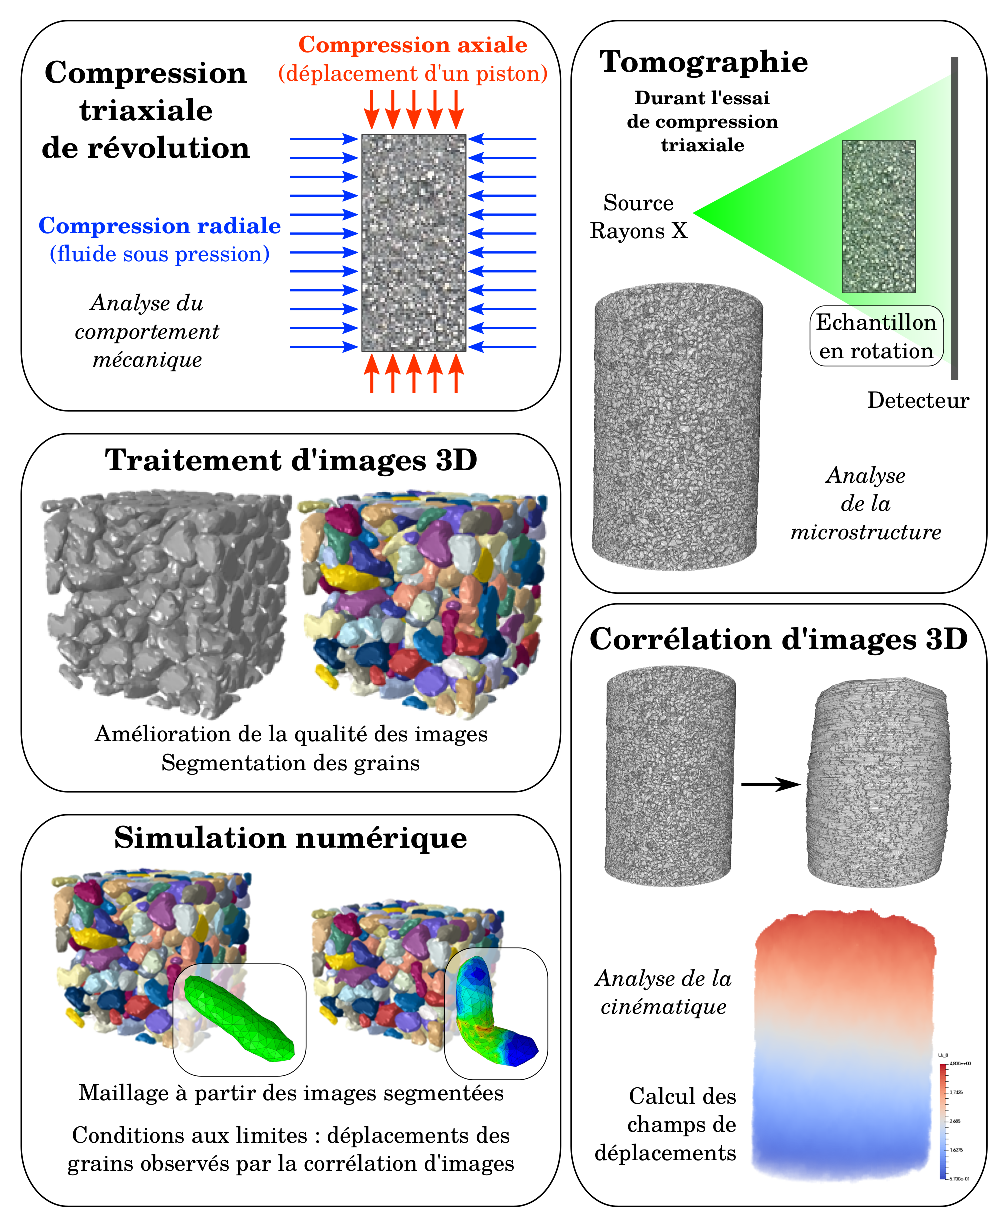
\includegraphics[width=0.95\textwidth]{method.eps}
	\caption{\label{fig:02-method}Les différentes étapes des travaux réalisés}
\end{figure}
	\graphicspath{{./03-Biblio/images/}}

\chapter{Analyses multi-échelles des milieux granulaires}
\label{chap:biblio}

%\epigraph{Si chacun de nous ajoute quelque chose au domaine commun, dans l'ordre de la science, de l'art ou de la moralité, c'est parce qu'une longue série de générations ont vécu, travaillé, pensé et souffert avant nous.}{Marcellin \textsc{Berthelot}, chimiste français (1827 - 1907)}

L'objectif du présent chapitre est de présenter certaines des connaissances déjà acquises et de décrire quelques travaux réalisés par la communauté scientifique dans les domaines de la mécanique des milieux granulaires, du traitement d'images issues de techniques d'imagerie 3D et de la simulation numérique de compression de poudres.
\\Dans un premier temps une analyse des phénomènes physiques propres aux matériaux granulaires sera faite et une description des poudres utilisées dans les expérimentations sera donnée. Ensuite, une présentation de la tomographie à rayons X, technique d'imagerie 3D, sera faite avant de décrire plus en détails les principes des travaux réalisés sur les images 3D. Enfin, les principales méthodes de simulation numérique concernant les matériaux granulaires seront présentées afin de mieux connaître les tenants et les aboutissants de chacune d'entre elles.

\section{Milieux granulaires}
	Les paragraphes qui suivent servent aux lecteurs non avisés concernant les milieux granulaires. Il s'agit de décrire certains phénomènes physiques en liaison avec ces milieux de manière à mieux les comprendre. Ce qui suit est basé sur les lectures de \citet{mollon_mecanique_2015}, \citet[Chapitres 1, 4 et 5]{matuttis_understanding_2014} et \citet{cambou_micromechanics_2009}.
	\subsection{Matériaux granulaires}
		\subsubsection{Quelques chiffres}
			Bien qu'on n'y fasse pas vraiment attention, les matériaux granulaires sont très présents dans nos vies. Chaque année dans le monde, l'industrie manipule plusieurs milliards de tonnes de matériaux granulaires. Un matériau granulaire intervient dans le cycle de fabrication d'un produit fini sur deux et la matière en grain représente, en masse, \si{70}{\%} des matières premières de l'industrie mondiale \citep{thomas_poudres_2012}. Par ailleurs, l'Union Nationale des Producteurs de Granulats estime qu'en $2016$ la production de granulats (matériaux pour la construction) en France était de \num{5.1} tonnes par habitant \citep{unpg}. On voit ici l'importance économique que porte ces matériaux et pourtant, il est encore aujourd'hui difficile de comprendre le comportement de ceux-ci. Il s'agit donc d'un important levier économique.
			\\Les matériaux granulaires ont également une grande importance en ce qui concerne les enjeux humains puisqu'environ \num{32000} victimes par an dans le monde sont à déplorer à cause de glissements de terrain \citep{petley_global_2012}. On comprend alors l'intérêt suscité dans le domaine du génie civil à la compréhension de ces matériaux.
		\subsubsection{Applications industrielles et thématiques de recherche}
			Comme mentionné dans le précédent paragraphe, les matériaux granulaires sont utilisés par de très nombreuses industries. Les principaux secteurs sont mentionnés ci-dessous.
			\begin{itemize}
				\item Industrie minière : extraction de matières premières dans les carrières et les mines.
				\item Génie civil : fabrication du ciment, interactions entre constructions et sols, terrassement.
				\item Industrie agroalimentaire : production de matière en grains (céréales, aliments en poudres, fruits, ...).
				\item Industrie pharmaceutique : broyage, mélange et compaction de produits actifs et excipients.
				\item Industrie chimique : réactions solides-solides et solides-liquides (grande surface d'échange liée à la surface spécifique des grains)
				\item industrie mécanique : compression de poudre, traitement et convoyage de petites pièces en grande quantité.
			\end{itemize}
			Au delà des industries, de nombreuses recherches sont menées afin de répondre à certaines problématiques environnementales et humaines liées aux matériaux granulaires. En voici quelques exemples :
			\begin{itemize}
				\item Catastrophes humaines et matérielles par instabilités de pentes, activités volcaniques et sismiques. Les instabilités de terrains (glissements de terrains, avalanches) sont des écoulements granulaires et des efforts sont faits pour comprendre leurs déclenchement, propagation et arrêt. Les coulées volcaniques, sont des écoulements aérosols avec des températures et vitesses élevées. Encore une fois, la dynamique de ces coulées fait l'objet de nombreuses recherches. Enfin, un gros effort est également fourni afin de comprendre la propagation des ondes dans les matériaux granulaire pour mieux comprendre les phénomènes sismiques. Quoi qu'il en soit, de gros moyens sont mis en place afin de mettre en \oe{}uvre et dimensionner des systèmes de protection.
				\item \'Etude de la dynamique fluviale, littorale et des dunes de sable par sédimentologie. Les interactions entre fluide et milieu granulaire sont étudiés afin de comprendre l'équilibre dynamique dans le domaine de l'hydrologie. De même pour les interactions, complexes, entre topographie et climat pour comprendre la formation et le déplacement des dunes de sable.
				\item Compréhension de phénomènes physiques. La compréhension de phénomènes propres aux milieux granulaires (ségrégation, formation de motifs périodiques, corrugation, ...) est à l'origine de nombreuses études souvent simplifiées à l'extrême (grains sphériques de même taille). Enfin, les planétologues font souvent appel à l'étude de la matière en grains afin de mieux comprendre les cratères d'impacts, les anneaux de Saturne ou encore optimiser le déplacement des rovers sur les sols des planètes explorées.
			\end{itemize}
	\subsection{Mécanique des milieux granulaires confinés}
		\subsubsection{Propriétés et spécificités}
			En sciences des matériaux, on entend parler de trois états de la matière : l'état solide, l'état liquide et l'état gazeux. Le but ici n'est pas de décrire chacun de ces états de la matière mais de comprendre où placer les milieux granulaires qui sont constitués de particules solides mais qui s'écoulent à la manière des liquides. La matière en grains a en effet des propriétés très différentes de la matière dite continue. Ces spécificités, d'ordre géométrique, mécanique et physico-chimique, sont à l'origine des difficultés de modélisation rencontrées lorsqu'on s'intéresse aux matériaux granulaires.
			\\La première spécificité des milieux granulaires est qu'il n'existe pas d'équation universelle comme pour les matériaux plus "classiques". En effet, l'élasticité donne la loi de Hooke pour les matériaux solides déformables. Il en va de même avec l'équation de Navier-Stokes pour les fluides newtoniens. Quand ces matériaux continus ne sont pas élastiques et que les fluides sont non-newtoniens, il est possible de faire évoluer ces lois en ajoutant des paramètres par exemple. En ce qui concerne les matériaux granulaires, il n'existe pas encore de loi universelle du comportement de la matière. On se base donc généralement sur des fondements empiriques et sur des théories plus ou moins abouties souvent contraignantes (géométrie des grains, régime d'écoulement, loi de contact, type de matériau).
			\\Le grand nombre de particules dans un tel milieu le rend également spécifique. Le fait d'être en présence d'un très grand nombre de solides de très petites tailles engendre une surface de contact accessible totale, appelée surface spécifique, très grande. Du fait de cette caractéristique, de très nombreux contacts physiques et interactions physico-chimiques s'établissent entre les particules. Cela rend le milieu granulaire plus complexe à étudier. Par exemple, les approches macroscopiques basées sur la conservation d'énergie ne sont plus valables puisque le milieu dissipe énormément d'énergie à l'échelle des grains.
			\\Enfin, il existe une autre spécificité du milieu granulaire : il est difficile de séparer l'échelle du grain de l'échelle globale du système de grains. En ce qui concerne les matériaux continus plus classiques, les chercheurs et ingénieurs s'intéressent très souvent à des comportements significatifs qui se situent à une échelle très largement supérieure à celle des particules élémentaires. Dans les milieux granulaires, il est très difficile d'étudier un ensemble de particules de manière exacte en ignorant soit l'échelle des particules, soit l'échelle globale du système. En voici un exemple : une bande de cisaillement d'épaisseur équivalente à quelques grains peut engendrer le glissement de plusieurs millions/milliards de grains se situant d'un côté ou de l'autre de la bande de glissement. Le phénomène est ici à la fois local (bande de cisaillement étroite) et global (déplacement d'une grande masse de particules).
		\subsubsection{Phénoménologie}
			On peut, de manière générale, considérer deux grandes familles de matériaux granulaires qui dépendent de la taille et de la nature des particules constituant le milieu :
			\\\vspace{1mm}\\
			\begin{minipage}[c]{0.24\linewidth}
				\includegraphics[width=\textwidth]{poudre_fine_shipton-mill.jpg}
			\end{minipage}\hfill
			\begin{minipage}[c]{0.74\linewidth}
				\begin{itemize}
					\item \emph{Les milieux granulaires "fins" ou poudres} dont les particules sont de tailles inférieures ou approximant le micromètre. Des forces cohésives existent généralement entre les particules (Van Der Waals, électrostatiques, capillaires) et les interactions avec le fluide environnant (eau, air, ...) sont à prendre en compte. L'étude des poudres nécessite de prendre en compte la physico-chimie en plus de l'approche purement mécanique. (Source photo : \url{www.shipton-mill.com}).
				\end{itemize}
			\end{minipage}\vspace{5mm}
			\begin{minipage}[c]{0.24\linewidth}
				\includegraphics[width=\textwidth]{graviers_unpg.jpg}
			\end{minipage}\hfill
			\begin{minipage}[c]{0.74\linewidth}
				\begin{itemize}	
					\item \emph{Les milieux granulaires "grossiers"} dont les particules ont des tailles généralement supérieures à la centaine de micromètres. Les grains vont alors être soumis à la gravité et aux forces de contacts des particules voisines (appuis, frottements, chocs). Une approche purement mécanique suffit à étudier le milieu. Malgré cette avantage par rapport aux poudres fines, il reste difficile de bien comprendre ces milieux pulvérulents. (Source photo : \url{www.unpg.fr})
				\end{itemize}
			\end{minipage}\vspace{5mm}
			En fonction de la famille d'appartenance du milieu granulaire, certains phénomènes sont à prendre en compte et d'autres non. Les paragraphes qui suivent donnent une liste de ces phénomènes. Comme ces derniers dépendent de nombreux paramètres, il ne sera pas spécifié les conditions d'obtention de manière précise mais plutôt de manière générale.
			\subparagraph{Interactions en surface -}
				Pour les particules les plus grossières, l'interaction entre surfaces de grains est principalement due à la déformation élastique pour la composante normale et à la friction de Coulomb pour la composante tangentielle. Lorsque les particules sont plus fines, d'autres interactions peuvent intervenir. Dans un environnement fortement humide, les petits grains vont interagir entre eux par l'intermédiaire d'une force de cohésion liée à l'agglomération de molécules d'eau au niveau des contacts. Dans un environnement sec en revanche, des effets électrostatiques peuvent apparaître s'il existe un mouvement relatif entre les grains. Tous ces effets de surface vont avoir une importance cruciale sur le comportement du milieu granulaire. Il est à noter que ces interactions sont dépendantes de la taille des grains\footnote{Cela ne concerne pas les forces "mécaniques" mais plutôt les forces d'adhésion (capillaires, Van der Waals, ...).}, de leur nature et de l'environnement. Si la nature des grains reste invariante, l'environnement et la taille des grains, eux, peuvent varier au cours du temps (climat, fractures des grains, frittage, ...).
			\subparagraph{Friction et dissipation d'énergie -}\label{para03:friction}
				Les effets de friction et de dissipation contribuent aux interactions entre grains mais mènent également à des comportements macroscopiques qui diffèrent de celui des systèmes d'atomes et de molécules. Dans un milieu dense, les frottements aux interfaces du milieu granulaire joue un rôle important et expliquent par exemple les effets d'arche qui seront présentés dans un prochain paragraphe.
			\subparagraph{Géométrie des particules, roulement et glissement -}\label{para03:glissement}
				En fonction de la géométrie des grains, le comportement du milieu granulaire peut drastiquement changer. Ici le terme géométrie décrit uniquement la forme des grains et non leur taille. Le fait que les particules aient des formes complexes ou non va également jouer sur le comportement du milieu. Un milieu constitué uniquement de grains sphériques facilitera l'analyse (puisqu'on peut considérer les symétries et diminuer le nombre de variables pour la modélisation) mais sera moins approprié pour l'étude de certains phénomènes physiques. En effet, pour des particules sphériques les surfaces de contact sont minimisées et les effets liés à la friction et à la cohésion seront également minimisés puisque les efforts de contact seront normaux aux surfaces. Ainsi, un tel milieu mettra l'accent sur le roulement aux dépends du glissement si aucun coefficient de frottement n'est considéré. Lors d'un réarrangement de grains, la dissipation d'énergie est minimale. \`A l'inverse, un milieu pour lequel les particules ont des formes complexes présentera des surfaces de contacts également plus complexes et il existe naturellement un équilibre entre glissement et roulement. De tels milieux vont permettre d'observer ce qui a été décrit dans le paragraphe précédent sur la friction et la dissipation d'énergie. Cet effet est observable sur la figure \ref{fig03:shape_effect}.
				\begin{figure}\centering
					\begin{minipage}[c]{0.47\textwidth}
						\subfloat[]{
							\includegraphics[width=\textwidth]{heap_hex.png}
							\label{subfig03:shape_effect_hex}
						}
					\end{minipage}\hspace{0.04\textwidth}
					\begin{minipage}[c]{0.47\textwidth}
						\subfloat[]{
							\includegraphics[width=\textwidth]{heap_circ_init.png}
							\label{subfig03:shape_effect_circ_init}
						}\\
						\subfloat[]{
							\includegraphics[width=\textwidth]{heap_circ_final.png}
							\label{subfig03:shape_effect_circ_final}
						}
					\end{minipage}
					\caption{\label{fig03:shape_effect}Effet de la forme des particules sur la formation d'un tas : (a) les particules polyédriques se stabilisent grâce à l'effet de la friction lors du glissement ;  (b) lorsqu'un empilement de particules sphériques et créé, (c) ces dernières roulent sans glisser et se dispersent dans l'espace \citep{matuttis_understanding_2014}.}
				\end{figure}
			\subparagraph{Effet d'arche -}
				L'effet d'arche se caractérise lorsque des forces normales à la direction de chargement apparaissent. Dans les milieux granulaires, ce phénomène est très présent et est utilisé depuis des milliers d'années dans la construction. Lorsque le milieu granulaire est confiné entre des parois, les grains vont engendrer des forces liées au frottement grain/grain et grain/paroi. Ces forces vont être propagées de grain en grain formant ce qu'on appelle une chaîne de forces. Le chemin suivi par les chaînes de forces dépend des contacts qui existent entre les grains (nombre, surface et direction des contacts). En général, les chaînes de forces dévient rapidement de la direction de sollicitation produisant ainsi des forces radiales. Cet effet explique l'importance des efforts de frottements entre un ensemble de grains soumis à son propre poids et les parois d'un silo à grain.
			\subparagraph{Dilatance de Reynolds -}\label{para03:dilatance}
				Le phénomène de dilatance est observable dans un milieu granulaire en compression dans lequel des contraintes de cisaillement sont présentes. Il est possible d'illustrer le phénomène par un essai de compression triaxiale (\textit{c.f.} paragraphe \ref{para03:triax}) bien que la dilatance se manifeste dans d'autres cas. Lors d'un confinement isotrope, les grains se réarrangent et se déforment de la même manière quelque soit la direction (en moyenne en tout cas) : il y a une densification du milieu (volume qui diminue et résistance mécanique qui augmente). Si maintenant la compression augmente suivant une direction mais reste constante suivant les autres (pression de confinement constante avec chargement axial), alors les grains, qui se déplacent majoritairement dans l'axe de compression, sont confrontés à deux types de résistances : les forces de frottements intergranulaires et la résistance liée au manque d'espace avec les grains voisins. Lorsque l'effort de cisaillement est suffisamment grand pour contrecarrer ces résistances au mouvement, un réarrangement des grains se fait remarquer. C'est ce réarrangement, moins ordonné, des grains qui génère une augmentation du volume qui correspond au phénomène de dilatance. La figure \ref{fig03:dilatance} aide à comprendre le réarrangement des grains lorsque des efforts de cisaillement interviennent. La dilatance dans un milieu granulaire est également une des causes de l'effet d'arche.
				\begin{figure}\centering
					\begin{minipage}[c]{0.4\textwidth}\centering
						\begin{tikzpicture}[scale=.5]
							% Dessine le volume
							\fill[gray!40] (-1.5,-1.5) rectangle ++(10.5,{3+3*sin(60)});
							\begin{scope}
								\clip (-1.5,-1.5) rectangle ++(10.5,{3+3*sin(60)});
								% Dessine les grains du bas
								\filldraw[ball color=blue!50] (0,0) circle (1.5);
								\filldraw[ball color=red!50] (3,0) circle (1.5);
								\filldraw[ball color=purple!50] (6,0) circle (1.5);
								\filldraw[ball color=orange!50] (9,0) circle (1.5);
								% Dessine les grains du haut
								\filldraw[ball color=purple!50] (120:3) circle (1.5);
								\filldraw[ball color=orange!50] (60:3) circle (1.5);
								\filldraw[ball color=yellow!50] (3,0) ++(60:3) circle (1.5);
								\filldraw[ball color=green!50] (6,0) ++(60:3) circle (1.5);
							\end{scope}
							% Dessine le cadre du volume et écrit
							\draw [ultra thick, dashed] (-1.5,-1.5) rectangle ++(10.5,{3+3*sin(60)});
							\path (4,{2.5+3*sin(60)}) node [above]{Volume $\mathcal{V}$};
							% Dessine le chargement
							\foreach \x in {8.9,7.4,...,-0.1} {
								\draw[very thick, -latex, red] (\x,{2+3*sin(60)}) -- ++(-1.3,0);}
							\foreach \x in {-1.4,0.1,...,7.6} {
								\draw[very thick, -latex, red] (\x,-2) -- ++(1.3,0);}
						\end{tikzpicture}
					\end{minipage}
					\begin{minipage}[c]{0.18\textwidth}\centering
						~\\\vspace{5mm}~\\
						\begin{tikzpicture}
							\draw[thick, ->] (0,0) -- (3,0) node[midway, above] {Chargement au} node[midway, below]{cours du temps};
						\end{tikzpicture}
					\end{minipage}
					\begin{minipage}[c]{0.4\textwidth}\centering
						\begin{tikzpicture}[scale=.5]
							% Dessine le volume
							\fill[gray!40] (-1.5,-1.5) rectangle ++(10.5,6);
							\begin{scope}
								\clip (-1.5,-1.5) rectangle ++(10.5,6);
								% Dessine les grains du bas
								\filldraw[ball color=green!50] (-3+.75,0) circle (1.5);
								\filldraw[ball color=blue!50] (0.75,0) circle (1.5);
								\filldraw[ball color=red!50] (3.75,0) circle (1.5);
								\filldraw[ball color=purple!50] (6.75,0) circle (1.5);
								\filldraw[ball color=orange!50] (9.75,0) circle (1.5);
								% Dessine les grains du haut
								\filldraw[ball color=purple!50] (-3+.75,3) circle (1.5);
								\filldraw[ball color=orange!50] (.75,3) circle (1.5);
								\filldraw[ball color=yellow!50] (3.75,3) circle (1.5);
								\filldraw[ball color=green!50] (6.75,3) circle (1.5);
								\filldraw[ball color=blue!50] (9.75,3) circle (1.5);
							\end{scope}
							% Dessine le cadre du volume et écrit
							\draw [ultra thick, dashed, red] (-1.5,-1.5) rectangle ++(10.5,6);
							\path (4,5) node [above]{Volume ${\color{red}\mathcal{V^*}} > \mathcal{V}$};
						\end{tikzpicture}
					\end{minipage}
					\caption{\label{fig03:dilatance}Illustration du phénomène de dilatance : l'état initial (à gauche) est plus dense que l'état après chargement (à droite). Cela ne se produit que pour des efforts de cisaillement assez importants au sein du milieu granulaire.}
				\end{figure}
			\subparagraph{Formation de bandes de cisaillement -}\label{para03:bande_cisaillement}
				Lorsqu'un milieu granulaire est comprimé de manière non isotrope, des contraintes de cisaillement font leur apparition dans certaines zones. Comme il l'a été dit dans le paragraphe précédent, l'apparition de contraintes de cisaillement dans un milieu confiné engendre également un effet de dilatance. Ainsi, dans les zones où les contraintes de cisaillement atteignent une valeur relativement grande, les grains vont avoir tendance à se désenchevêtrer et diminuer la densité du milieu localement. Généralement cela se passe sur un plan ayant une épaisseur de quelques grains qu'on appelle bande de cisaillement. Lorsque la densité diminue, la résistance mécanique diminue également et les zones de cisaillement deviennent finalement les zones de rupture, on entend souvent parler de bande de glissement puisqu'une partie située d'un côté de la bande va glisser sur la partie située de l'autre côté. La figure \ref{fig03:cisaillement} montre l'apparition d'une bande de cisaillement observée par tomographie à rayons X (cf. paragraphe \ref{para03:tomo}) lors d'un essai de compression triaxiale (cf. paragraphe \ref{para03:triax}). La figure \ref{subfig03:cisaillement_02} est issue de la corrélation d'images 3D (cf. paragraphe \ref{para03:DIC}) et montre les déformations déviatoires permettant ainsi de distinguer clairement la bande de cisaillement.
			\begin{figure}\centering
				\subfloat[]{
					\includegraphics[height=0.3\linewidth]{bande_cisaillement_00.jpg}
					\label{subfig03:cisaillement_00}}\hspace{1.5cm}
				\subfloat[]{
					\includegraphics[height=0.3\linewidth]{bande_cisaillement_01.jpg}
					\label{subfig03:cisaillement_01}}\hspace{1.5cm}
				\subfloat[]{
					\includegraphics[height=0.26\linewidth]{bande_cisaillement_02.jpg}
					\label{subfig03:cisaillement_02}}
				\caption{\label{fig03:cisaillement}Reconstructions de tomographie montrant la formation d'une bande de cisaillement dans un ensemble de grains (a) à l'état initial avant chargement et (b) à l'état final après chargement. (c) On distingue encore mieux la bande grâce à la corrélation d'images (illustrations issues des travaux de  \cite{kawamoto_all_2018}).}
			\end{figure}
	\subsection{Essais de compression dédiés aux milieux granulaires}
		De manière générale, les matériaux granulaires ne forment plus un système solide à partir d'une certaine contrainte en traction qui élimine tout effort de cohésion intergranulaire. C'est la raison pour laquelle l'étude de ces milieux en équilibre statique s'intéresse en grande partie aux états confinés. On retrouvera certains éléments qui suivent dans les lectures de \citet{terzaghi_soil_1996} et \citet{bardet_experimental_1997}.
		\subsubsection{Les essais de compression}
			Nous allons voir dans les paragraphes qui suivent, deux méthodes couramment utilisées pour étudier le comportement mécanique des poudres dans des espaces confinés. Ces essais sont bien connus des géotechniciens qui caractérisent les sols régulièrement avec ces techniques. Nous considérerons que l'échantillon est axisymétrique (d'où les termes "de révolution") et que la direction axiale est la direction de l'axe de symétrie tandis que les directions radiales sont les directions normales à cet axe. Lorsqu'on s'intéresse à la mécanique des milieux granulaires, il est plus facile d'utiliser la convention utilisée en géotechnique qui consiste à considérer les contraintes de compression positives alors que la traction est négative.
			\paragraph{Compression \oe{}dométrique de révolution\\}
				L'essai de compression \oe{}dométrique est également appelé essai de consolidation ou de compressibilité. Il permet d'apprécier la déformation axiale d'un échantillon dont les parois latérales sont fixes et rigides de manière à ne pas se déformer sous l'action des efforts traversant l'échantillon. Un schéma de principe est donné sur la figure \ref{fig03:oedometre}. Avec cet essai, la déformation de l'échantillon est uniquement axiale et il est possible de mesurer la force appliquée dans la direction axiale, le déplacement appliqué dans la même direction mais aussi dans certains cas la pression exercée par l'échantillon sur les parois latérales. Ainsi, en reprenant les notations fournies à la page \pageref{keywords}, après mise en chargement on a :
				\begin{equation}\label{eq03:defo_oedometre}
					\left\{\begin{array}{l}
						\varepsilon_a (= \varepsilon_{33}) \neq 0\\
						\varepsilon_r (= \varepsilon_{11} = \varepsilon_{22}) = 0\\
						\gamma_{12} = \gamma_{13} = \gamma_{23} = 0
					\end{array}\right.
				\end{equation}
				\begin{figure}\centering
					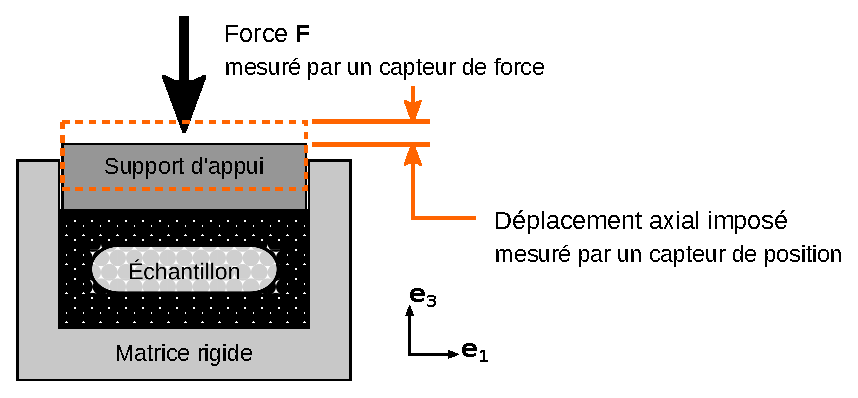
\includegraphics[scale=0.9]{oedometre.eps}
					\caption{\label{fig03:oedometre}Principe du test de consolidation}
				\end{figure}
				Cet essai peut également être réalisé avec drainage. La circulation d'un fluide est alors permise et ce dernier est drainé vers l'extérieur du moule. Cela permet d'observer l'effet du tassement sur un milieu plus ou moins saturé (exemple : un sol saturé en eau).
			\paragraph{Compression triaxiale de révolution\\}\label{para03:triax}
				De manière générale un matériau granulaire est dans un état confiné. Cela veut dire que la contrainte moyenne dans le milieu constitue un état de compression, donc positive. Par décomposition du tenseur des contraintes (\ref{eq03:contraintes_triax}), on peut dire qu'il existe une contrainte de compression hydrostatique (donc isotrope), qui est la contrainte moyenne $p$, positive mais également des contraintes déviatoires qui modifient la géométrie du milieu. L'ensemble des contraintes déviatoires forme le déviateur des contraintes $\doubleunderline{\sigma_d}$. La contrainte déviatoire $q$ est couramment utilisée afin de déterminer la contribution des efforts qui ne modifient pas le volume du système. Par définition, cette contrainte déviatoire $q$ correspond à la contrainte équivalente de Von Mises calculée à partir du tenseur des contraintes déviatoires. Pour un système en contraintes axisymétriques (ce qui est le cas pour l'essai de compression triaxiale), $q$ correspond à la différence, en valeur absolue, de la contrainte axiale $\sigma_a$ et de la contrainte radiale $\sigma_r$. Si l'axe $3$ correspond à la direction axiale, alors:
				\begin{equation}\label{eq03:contraintes_triax}
					\begin{array}{l}
						\doubleunderline{\sigma} = p\cdot\doubleunderline{I} + \doubleunderline{\sigma_d}\\
						\\
						q = \sqrt{\cfrac{3}{2}\;\mathrm{tr}(\doubleunderline{\sigma_d}^2)}
					\end{array}
					\quad\text{avec}\quad\begin{array}{rcl}
					p & = & \text{tr}(\doubleunderline{\sigma})/3\vspace{0.3cm} = (\sigma_{11}+\sigma_{22}+\sigma_{33})/3\\
					\doubleunderline{\sigma_d} & = &
					\begin{pmatrix}
						\sigma_{11}-p & \sigma_{12} & \sigma_{13} \\
						\sigma_{12} & \sigma_{22}-p & \sigma_{23} \\
						\sigma_{13} & \sigma_{23} & \sigma_{33}-p \\
					\end{pmatrix}\end{array}
				\end{equation}
				\indent L'essai de compression triaxiale consiste à déterminer les états de contraintes et déformations de l'échantillon lorsque ce dernier est chargé de manière axiale et radiale. Le chargement axial se fait de la même manière que pour l'essai de compression \oe{}dométrique, un piston vient exercer une force à l'extrémité de l'échantillon. On peut choisir de piloter soit la force appliquée par le piston, soit la vitesse de déplacement du piston. Le chargement radial est quant à lui exercé par l'intermédiaire d'un fluide mis sous pression. En fait, le dispositif ne permet pas de créer un chargement uniquement radial en plus du chargement axial, il crée un chargement isotrope. Pour cela, une membrane souple est placée aux extrémités de l'échantillon de manière à l'isoler du fluide environnant, il faut donc une membrane étanche et suffisamment souple pour ne pas rigidifier l'échantillon. Le fluide qui englobe complètement l'échantillon est mis sous pression de manière à exercer cette pression sur la membrane, et donc sur le matériau à tester. La contribution de ce chargement est uniquement isotrope puisqu'il s'agit d'une pression hydrostatique. Un schéma du principe de l'essai est donné dans la figure \ref{fig03:triax}. Les membranes sont très souvent des membranes en élastomère (latex, néoprène, ...). L'eau ou l'huile sont régulièrement utilisés comme fluides mis en pression.
				\begin{figure}\centering
					\includegraphics[scale=0.9]{triax.eps}
					\caption{\label{fig03:triax}Principe de l'essai de compression triaxiale}
				\end{figure}
				\\La compression triaxiale de révolution à l'avantage d'être plus riche en terme d'information que l'essai de consolidation. En effet, le chargement radial étant imposé et l'échantillon étant accessible dans une cellule, il est possible d'obtenir la cinématique de l'ensemble et de connaître les efforts que subit la surface extérieure de l'échantillon, que ce soit dans les directions radiales ou axiale. Un autre avantage de cet essai par rapport à l'essai \oe{}dométrique est la possibilité de s'affranchir du frottement contre la paroi avec l'utilisation d'une membrane souple qui se déforme avec le milieu testé. On voit ici que la pression appliquée par le fluide influence la contrainte moyenne $p$ dans l'échantillon. Le chargement axial va, lui, influencer à la fois la contrainte moyenne $p$ mais aussi et surtout la contrainte déviatoire $q$. Ainsi, il est simple avec ce test de créer plusieurs chemins de chargement afin d'observer les effets de la contrainte moyenne de compression et de la contrainte déviatoire.
				\\Contrairement à la compression \oe{}dométrique où l'on observe la relation (\ref{eq03:defo_oedometre}), dans le cas de l'essai triaxial, si l'axe $3$ correspond à la direction axiale, on a :
				\begin{equation}\label{eq03:defo_triax}
					\left\{\begin{array}{l}
						\varepsilon_a (=\varepsilon_{33}) \neq 0\\
						\varepsilon_r (=\varepsilon_{11} =\varepsilon_{22}) \neq 0\\
						\gamma_{13} = \gamma_{23} \neq 0\\
						\gamma_{12} = 0
					\end{array}\right.
				\end{equation}
				Il est possible de décomposer le tenseur des déformations de la même manière que pour le tenseur des contraintes. Ainsi, nous parlerons de la déformation volumique $\varepsilon_v$ qui définit la part des déformations qui modifient le volume de l'échantillon et du déviateur des déformations $\doubleunderline{\varepsilon_d}$ qui définit les déformations impliquant un changement de géométrie de l'échantillon. On aura tendance, plus particulièrement, à parler de la déformation déviatoire $\varepsilon_d$ qui est définie de la manière indiquée ci-dessous. Si la direction \num{3} correspond à la direction axiale alors :
				\begin{equation}\label{eq03:decomposition_defo_triax}
					\begin{array}{l}
						\doubleunderline{\varepsilon} = \cfrac{1}{3}\;\varepsilon_v\cdot\doubleunderline{I} + \doubleunderline{\varepsilon_d}\\\\
						\varepsilon_d = \sqrt{\cfrac{2}{3}\;\mathrm{tr}(\doubleunderline{\varepsilon_d}^2)}
					\end{array}
					\quad\text{avec}\quad\begin{array}{rcl}
					\varepsilon_v & = & \text{tr}(\doubleunderline{\varepsilon})\vspace{0.3cm} = \varepsilon_{11}+\varepsilon_{22}+\varepsilon_{33}\\
					\doubleunderline{\varepsilon_d} & = &
					\begin{pmatrix}
					\varepsilon_{11}-\varepsilon_v/3 & \gamma_{12} & \gamma_{13} \\
					\gamma_{12} & \varepsilon_{22}-\varepsilon_v/3 & \gamma_{23} \\
					\gamma_{13} & \gamma_{23} & \varepsilon_{33}-\varepsilon_v/3 \\
					\end{pmatrix}\end{array}
				\end{equation}
				Pour des petits incréments de déformation, la déformation volumique $\varepsilon_v$ donne une très bonne approximation du rapport $(\mathrm{d}V-\mathrm{d}V_0)/\mathrm{d}V$ avec $\mathrm{d}V_0$ et $\mathrm{d}V$, respectivement, les volumes élémentaires avant et après déformation.
				\\\indent Comme avec le test de consolidation, il est possible d'observer l'effet du drainage d'un fluide circulant dans l'échantillon. On parlera d'essai de compression triaxiale drainé lorsque c'est le cas, ou non drainé dans le cas contraire.
		\paragraph{Compression de particules ductiles\\}
			Le comportement mécanique des particules qui constituent un milieu granulaire joue un rôle important dans le comportement mécanique de l'ensemble du milieu. C'est en effet la réponse mécanique de chacun des grains qui va dicter la réponse de l'ensemble de grains.
			\\Lorsque des particules présentant une rigidité élevée sont introduites et comprimées dans un moule et qu'elles ne sont pas soumises à des efforts engendrant leur fracture, ce sont essentiellement les chaînes de forces qui se créent dans le milieu qui va dicter la réponse mécanique du milieu granulaire. Dans ce cas, la géométrie des grains et la friction entre les grains et les parois du moule sont des facteurs très influents concernant les propriétés mécaniques du milieu.
			\\Dans le cas où le milieu pulvérulent est constitué de grains ductiles, c'est à dire capables de se déformer assez largement à un certain niveau de contraintes, alors la déformation des grains joue un rôle crucial dans la réponse mécanique de l'ensemble de grains. En effet, l'énergie de déformation nécessaire à la déformation des particules prend part dans le bilan énergétique et certains phénomènes vont être plus ou moins marqués. Par exemple, \citet{pavier_caracterisation_1998} montre que la dilatance de Reynolds est difficile à observer dans le cas d'un matériau constitutif ductile. En l'absence d'une surconsolidation élevée, la déformation des grains sous cisaillement permet le glissement des grains entre eux sans avoir à s'écarter. Les déformations vont être les plus grandes au niveau des zones de contact puisqu'il s'agit des zones où les contraintes sont le plus présentes. Ces déformations, au niveau des zones de contacts, vont élargir les surfaces de contacts et les effets liés aux frottements des grains vont être moins présents puisque les glissements inter-grains sont alors plus limités.
		\paragraph{}
			Il a été précédemment montré l'importance de la nature des particules constituant le milieu granulaire sur son comportement mécanique. Il est donc essentiel de connaître les propriétés du matériau constitutif afin de comprendre le comportement d'un système de grains. La partie qui suit à pour objectif de présenter les propriétés du matériau utilisé dans les travaux présentés ici : le polystyrène.
	\subsection{Comportement des particules polymériques}
		Cette partie a pour objectif de présenter le matériau granulaire concerné dans cette thèse. Comme il l'a été expliqué au chapitre \ref{chap:intro}, l'étude portera uniquement sur le matériau modèle et non sur des grains d'amidon, qui historiquement constituait le matériau d'étude. Afin d'informer le lecteur sur le matériau amidon, l'annexe \ref{annexe:amidon} présente les principales propriétés de celui-ci. Les propriétés mécaniques de l'amidon peuvent être analysées afin de déterminer les similitudes et différences avec le matériau modèle présenté ci-dessous.
		\\Les particules étudiées dans les travaux qui suivent sont des grains de polystyrène (pouvant être abrégé "PS" par la suite). Le polystyrène a un comportement mécanique typique des polymères. Avant de commencer à présenter ce matériau, une courte explication du comportement des polymères est nécessaire.
		\subsubsection{Polymères}
		Un polymère est un matériau organique constitué d'un ensemble de macromolécules, elles-mêmes constituées d'un certain enchaînement d'éléments structurants, appelés monomères, composés de chaînes carbonées. Les matériaux polymères font partie d'une très grande famille de matériaux. Il existe différentes sous-familles de polymères : le classement trouvé le plus souvent dans les ouvrages différencie les thermoplastiques, les thermodurcissables et les élastomères. Il s'agit là d'un classement assez global qui tient compte de nombreuses propriétés thermomécaniques : les thermoplastiques, une fois chauffés, sont malléables et facilement mis en forme, les thermodurcissables durcissent de manière irréversible sous l'action de réactifs et/ou d'un environnement favorisant (chaleur, lumière, ...) et les élastomères sont capables de se déformer de manière réversible jusqu'à de grandes, voire très grandes, déformations. Il est également possible de différencier les polymères par d'autres moyens : nature chimique, "forme" de la macromolécule, formulation chimique, arrangement cristallographique, etc. De par leurs natures très variées, les polymères peuvent avoir des comportements mécaniques très différents. De manière générale, les propriétés mécaniques des polymères dépendent d'au moins deux facteurs :
		\begin{itemize}
			\item le temps : les relations entre contraintes $\sigma$ et déformations $\varepsilon$ sont dépendantes de la vitesse de chargement $\dot{\sigma}$ et de la vitesse de déformation $\dot{\varepsilon}$. Cette propriété introduit le caractère visqueux des polymères.
			\item la température : il existe des transitions de phases pour certaines températures. Par exemple, la température de transition vitreuse définit les intervalles de températures pour lesquelles le matériaux passe d'un état caoutchouteux à un état de solide rigide. Le caractère visqueux des polymères est très dépendant de la température.
		\end{itemize}
		On ne peut pas dire qu'un matériau polymère soit un matériau répondant uniquement à la loi de Hooke, à la théorie de la plasticité ou à la loi de la viscosité des fluides. Afin d'étudier ces matériaux, il est plutôt judicieux de s'intéresser à la viscoélasticité et la viscoplasticité pour mieux comprendre l'écoulement des polymères : on entre dans le domaine d'étude de la rhéologie. Plusieurs modèles rhéologiques existent pour décrire au mieux le comportement des polymères.
		\subsubsection{Polystyrène (PS)} \label{para03:PS}
			Le polystyrène est un polymère semi-cristallin qui constitue le milieu granulaire étudié dans cette thèse dont l'utilisation et la conservation est faite à température ambiante (entre \SI{20}{\celsius} et \SI{25}{\celsius}), donc sous la température de transition vitreuse.
			Comme pour la majorité des polymères, le polystyrène est un matériau qui existe sous différentes formes. Même si les différentes structures macromoléculaires que peut avoir le PS rendent ce matériau polyvalent et élargissent les plages de données de ses propriétés physico-chimiques, la structure globale est basée sur un seul monomère de nature assez simple. Ainsi, les propriétés de ce thermoplastique s'expliquent aisément par l'interprétation de sa microstructure et de sa nature chimique. On trouve d'ailleurs facilement les caractéristiques de ce matériau dans des ouvrages se consacrant aux matériaux polymériques couramment utilisés dans l'industrie tel que le "Handbook of polymers" de \citet{wypych_handbook_2016}.
			\paragraph{Composition chimique -}
				Le polystyrène est composé d'un seul monomère : le styrène. Cette molécule, représentée sur la figure \ref{fig03:PS_structure}, est constituée d'une chaîne carbonée linéaire de deux atomes de carbone à laquelle est rattachée chimiquement un groupe phényle sur l'un de ces atomes. Sa formule chimique est $\textrm{C}_8\textrm{H}_8$.
				\begin{figure}\centering
					\includegraphics[width=0.15\linewidth]{PS_structure.png}
					\caption{\label{fig03:PS_structure}Composition chimique du monomère constituant le PS : le styrène}
				\end{figure}
			\paragraph{PS cristal -}
				En fonction de l'agencement et de la méthode de synthèse du polymère, il est possible de trouver le polystyrène sous plusieurs formes (expansé, extrudé, choc, ...). Le PS "cristal" est considéré dans cette thèse. Il est l'homopolymère issu du styrène (cf. figure \ref{fig03:PS_structure}). Le PS cristal est transparent, dur et sensible aux chocs. Il est utilisé pour former des pièces plus ou moins transparentes assez rigides mais capables de se déformer relativement bien avant de rompre à température ambiante. Ses propriétés mécaniques, qui sont détaillées dans le prochain paragraphe, sont proches de celles observées pour l'amidon.
			\paragraph{Propriétés physico-chimiques -}
				Ici, uniquement les propriétés de l'homopolymère seront présentées puisqu'il s'agit du polystyrène utilisé dans les travaux de cette thèse. Le PS cristal possède des propriétés relativement variées en fonction de son degré de polymérisation et de sa tacticité. Le degré de polymérisation correspond au nombre moyen de monomères dans une chaîne polymère, il caractérise donc la longueur de la chaîne. La tacticité est une propriété chimique d'une chaîne polymère ayant des groupes substituants : elle définit la disposition dans l'espace de chaque groupe substituant. Le polystyrène est très généralement atactique (répartition aléatoire des groupes phényles) mais il est également possible de le trouver comme syndiotactique (répartition alternative), il est plus rarement synthétisé en isotactique (répartition uniforme).
				\\Le taux de cristallinité va dépendre fortement de la tacticité du polystyrène puisque celle-ci décrit l'ordonnancement des macromolécules. Un PS atactique sera plutôt amorphe, un PS isotactique sera très cristallin et un PS syndiotactique aura un taux de cristallinité moyen. Cela va donc impacter de nombreuses autres propriétés comme les températures de changement de phase. Les propriétés données dans la suite seront celles du PS atactique, utilisé dans cette thèse.
				\\Le polystyrène fait partie de la famille de thermoplastiques. Il est issu de la pétrochimie et n'est pas biodégradable. Il a une densité de \SI{1.05}{\gram\per\centi\meter^3}. Sa température de fusion est de \SI{275}{\celsius} alors que sa température de transition vitreuse est très légèrement au-dessus de \SI{100}{\celsius}. Le polystyrène est résistant aux solutions acides, alcools et produits alcalins. Il est considéré comme inerte dans l'industrie agroalimentaire.
				\\Les principales propriétés mécaniques du PS sont présentées sur le tableau \ref{tab03:meca_PS}. Ces données sont issues de \citet{wypych_handbook_2016}. Il est à noter que de nombreux autres ouvrages renseignent les mêmes propriétés et que les écarts de valeurs sont faibles.
				\begin{table}\centering
					\begin{tabular}{rcl}
						\hline
						\textbf{Module d'Young} & $2.9$ - $3.5$ & \si{\giga\pascal}\\
						\textbf{Coefficient de Poisson} & $0.38$ & \\
						\textbf{Résistance en traction} & $40$ - $66$ & \si{\mega\pascal}\\
						\textbf{Résistance en compression} & $70$ & \si{\mega\pascal}\\
						\hline
					\end{tabular}
					\caption{\label{tab03:meca_PS}Principales propriétés mécaniques du polystyrène atactique}
				\end{table}
	
	\paragraph{}
	Puisque l'analyse de la compression du milieu granulaire porte sur des grains déformables, une analyse de la microstructure du milieu au cours du temps et pendant l'essai s'avère utile. En effet, c'est l'évolution de cette microstructure qui peut expliquer certains phénomènes mis en jeu lors de la compression de l'ensemble de grains. Suivre la microstructure consiste à suivre le mouvement des grains, mais également à évaluer les déformations locales et les phénomènes de fissurations. Afin d'observer la microstructure, des outils d'imagerie existent en laboratoire. Les outils utilisés dans cette thèse permettent une évaluation 3D et sont présentés dans la partie qui suit.
	
\section{Imagerie 3D des milieux granulaires}
	Afin de bien comprendre le comportement mécanique des milieux granulaires, il est nécessaire d'étudier leur microstructure avant, pendant et après chargement. En effet, le comportement d'un milieu granulaire dépend des micromécanismes mis en jeu lors du chargement mécanique. Ces micromécanismes peuvent être mieux compris en suivant la microstructure. Une méthode d'imagerie permettant de connaître la microstructure en 3D est expliquée ci-dessous. Les images issues de cette méthode devront être traitées afin de pouvoir les analyser, certaines méthodes de traitement d'image seront introduites. Pour finir, la connaissance de la microstructure et de son évolution au cours du temps permet d'établir un champs de déplacement par corrélation d'images. Un paragraphe permettra de comprendre cette corrélation d'images.
	\subsection{Tomographie à rayons X}\label{para03:tomo}
		La tomographie à rayons X est une technique d'imagerie basée sur l'absorption des rayons X et permettant d'obtenir une information suivant les trois dimensions de l'espace. Pour comprendre cette technique, il est nécessaire d'expliquer avant tout le principe des radiographies à rayons X. Une fois cela fait, le principe de la tomographie pourra être expliqué.
		\subsubsection{Radiographie à rayons X}
			Les rayons X correspondent à des ondes électromagnétiques dont la longueur d'onde est comprise entre \SI{10}{\nano\meter} et \SI{1}{\pico\meter}. Cette radiation a été découverte en 1895 par le premier détenteur du prix Nobel de physique, le physicien allemand Wilhelm R\"ontgen lorsqu'il menait des expériences sur des tubes à vide. R\"ontgen se rendit compte que les radiations issues du tube à vide permettaient d'illuminer un écran fluorescent, même lorsque certains obstacles étaient placés entre le tube et l'écran. Une plaque métallique suffisait quant à elle à bloquer le faisceau lumineux. Il supposa alors qu'en fonction du matériau présent dans le faisceau, une atténuation des ondes plus ou moins importante se fait remarquer. Suite à cela, il prit la toute première radiographie à rayons X en demandant à sa femme d'intercaler sa main devant l'écran. R\"ontgen s'aperçut alors que les os bloquaient les rayons et la bague métallique encore plus, contrairement aux tissus de la main. Ainsi, l'écran fit apparaître une grande zone claire (là où les rayons n'ont pas été bloqués) sur laquelle des zones sombres définissent la géométrie des os et de la bague.
			\\L'histoire de cette découverte permet à elle seule de comprendre le principe des radiographies à rayons X. Les radiographies sont ni plus ni moins des mesures, dans le plan du détecteur, de la quantité de photons issus de la source à rayons X et franchissant le détecteur dans un intervalle de temps donné. En d'autres termes, il s'agit d'une intégration de l'atténuation des rayons X dans la matière qui a été traversée sur le chemin parcouru par le faisceau rayonnant.
		\subsubsection{Absorption des rayons X}
			Les rayons X peuvent interagir de différentes manières avec la matière (réfraction, réflexion, diffraction, ...) mais l'interaction qui entre en compte dans l'imagerie par rayons X est l'absorption photoélectrique. Il existe une plage assez vaste de longueurs d'ondes concernant les rayons X. Les rayons de plus fortes énergies (les plus faibles longueurs d'ondes) sont appelés rayons X durs et ceux de plus faibles énergies sont appelés rayons X mous.
			\\L'absorption photoélectrique est un phénomène physique qui consiste en l'émission d'électrons par un matériau soumis à un bombardement de photons. Pour un atome de la matière, l'absorption d'un photon d'une certaine énergie va engendrer l'émission d'un électron de même énergie. L'effet d'absorption des photons est grandement facilité lorsque ceux-ci ont une énergie proche de celle des électrons présents sur la couche K des atomes de la matière (la couche d'électrons la plus proche du noyau). C'est l'effet de l'énergie de liaison de la couche K présenté par \citet{nielsen_elements_2011}. L'énergie de liaison des électrons de la couche K augmente avec le numéro atomique $Z$. Ainsi, l'absorption des ondes sera dépendante des constituants de la matière et de l'énergie du rayonnement émis.
			\\Pour une énergie de rayonnement donnée, l'absorption des rayons X issus de ce rayonnement augmente continûment avec le numéro atomique, jusqu'à une valeur seuil qui correspond au numéro atomique de l'atome pour lequel l'énergie de liaison des électrons dans la couche K est supérieure à l'énergie des photons. Une discontinuité apparaît au niveau de ce seuil puisque pour des atomes plus lourds les photons vont rebondir sur la couche K, qui est alors trop énergétique pour eux, et vont par conséquent être transmis plus facilement. Il y a donc une chute brutale de l'absorption des rayons au niveau du seuil. Prenons l'exemple d'un rayonnement dont l'énergie est de \SI{100}{\kilo\electronvolt}. Les éléments dont le numéro atomique est relativement faible absorberont d'autant plus les photons que leur énergie de liaison de la couche K est proche de \SI{100}{\kilo\electronvolt}. Ainsi, le radon dont l'énergie de liaison de la couche K vaut \SI{98.4}{\kilo\electronvolt} atténuera grandement le rayonnement. Si le constituant devient un peu plus lourd, considérons le francium d'énergie de liaison de la couche K \SI{101.1}{\kilo\electronvolt}, alors théoriquement l'absorption des photons sera très faible.
			\\De manière générale, pour un matériau dense donné, les rayons X les plus durs sont ceux qui pénétreront le plus facilement dans la matière car l'absorption est relativement faible. En effet, les rayons les plus durs ont une énergie élevée et il faut donc un numéro atomique très élevé pour que l'énergie de liaison dans la couche K soit proche de celle des photons. Pour un tel rayonnement, l'atténuation des ondes va donc varier en fonction de la quantité d'atomes plus ou moins lourds rencontrés par les photons.
			\\Si $I(x)$ est l'intensité d'un faisceau monochromatique (une seule fréquence) se propageant suivant $(Ox)$ dans un milieu ($x>0$) et $I_0$ l'intensité de ce même faisceau avant d'interagir avec le milieu ($x<0$), alors la loi de Beer-Lambert permet de définir $I(x)$ en fonction de $I_0$ :
			\begin{equation}\label{eq03:beer_lambert}
				I(x) = I_0\cdot\exp{(-\mu\cdot x)}
			\end{equation}
			où $\mu$ est le coefficient d'absorption est dépend de la matière constituant le milieu : densité massique, masse molaire et bien sûr un coefficient d'atténuation qui dépend du numéro atomique des atomes dans le milieu.
			\\En radiographie, pour un temps donné, le faisceau de rayons est orienté dans une direction $(Ox)$ avec une intensité $I_0$. Le faisceau traverse ensuite plus ou moins facilement la matière à analyser , d'épaisseur $x_0$, et un détecteur, placé à l'opposé de la source du rayonnement par rapport au milieu traversé, permet de lire l'intensité du faisceau en fonction des zones traversées déterminées par $y$ et $z$. On a donc, d'après l'équation (\ref{eq03:beer_lambert}), au niveau du détecteur :
			\begin{equation}\label{eq03:beer_lambert_radio}
				I(y,z) = I_0\cdot\exp{(-\mu(y,z)\cdot x_0)}
			\end{equation}
			Le signal lu par le détecteur dépend donc uniquement du coefficient d'atténuation $\mu$. Le champ bi-dimensionnel observé par radiographie indique donc comment évolue le coefficient $\mu$ dans le plan du détecteur et correspond par conséquent au champ d'absorption des rayons X. Globalement, si tout est mis en \oe{}uvre pour négliger l'absorption de l'air, ce champ dépend de la densité du milieu et de sa constitution atomique. Si un seul et même matériau est analysé, alors le champ obtenu par radiographie s'apparente au champs des densités.
		\subsubsection{Tomographie par rayons X}
			La tomographie est une méthode d'imagerie semblable à la radiographie. Cependant, contrairement à la radiographie, elle permet d'obtenir un champ tri-dimensionnel de l'absorption des rayons. Cette méthode d'imagerie non destructive connait une essor très important ces dernières années. Le principe de la tomographie consiste à faire de nombreuses radiographies sous différents angles selon un axe normal au faisceau, puis de reconstruire mathématiquement le champ en 3D à partir des différents champs en 2D. Afin de prendre des radiographies sous différents angles, il existe deux possibilités : soit la source et le détecteur de rayons X tournent autour de l'échantillon qui, lui, est fixe ; soit c'est l'échantillon qui tourne alors que la source et le détecteur sont fixes. Les scanners d'imagerie médicale sont généralement issus de la première catégorie tandis que les tomographes de laboratoires sont souvent issus de la seconde.
			\\Nous allons illustrer le principe de la tomographie et de la reconstruction des images à trois dimensions grâce aux figures \ref{fig03:principe_tomo} et \ref{fig03:reconstruction_tomo}. Nous allons ici considérer un échantillon de forme cylindrique, qui est fixe dans l'espace et contenant certaines hétérogénéités. Afin de faciliter la compréhension en éliminant une dimension de l'espace, nous nous placerons à une hauteur fixe de l'échantillon, sur une coupe transversale d'épaisseur équivalente à la taille de pixel fournie par le détecteur. Sur cette couche, l'échantillon présente des hétérogénéités qui absorbent plus ou moins les rayons X. La figure \ref{fig03:principe_tomo} permet de visualiser ce que perçoit le détecteur lors d'une prise de radiographie (on parle également de projection) pour deux positions différentes formant un angle droit avec le centre de l'échantillon. Il faut imaginer que la taille des voxels (équivalent des pixels en 3D) est normalement environ un millier de fois plus petite que la taille de l'échantillon. Il est facile de s'apercevoir que les deux radiographies ne sont pas identiques. On obtiendra, à chaque fois que l'échantillon subit une rotation sur son axe longitudinal, une projection différente. Théoriquement, deux radiographies prises à \SI{180}{\degres} l'une de l'autre seront identiques par effet miroir. C'est la raison pour laquelle il n'est généralement pas utile de faire tourner l'échantillon de plus de \SI{180}{\degres}.
			\\La figure \ref{fig03:reconstruction_tomo} illustre la manière de reconstruire le champ de dimension $3$ à partir de différents champs de dimension $2$\footnote{Afin d'être plus explicite, la figure présente plutôt un champ de dimension $2$ construit à partir de champs de dimension $1$. La généralisation se fait en imaginant le même processus sur plusieurs couches selon la direction normale à la page.}. Le reconstruction se base sur la superposition des différentes projections dans l'espace. Avec deux radiographies, la superposition sera "pauvre" en terme de signal mais en augmentant considérablement le nombre de projections la précision du signal ne cessera de grandir. Alors que la taille des voxels définit la résolution du capteur, et donc la qualité de l'image, le nombre de projections va également jouer sur la qualité de la reconstruction, on parle alors de résolution angulaire. De façon à améliorer la qualité de l'image obtenue, il est courant de moyenner une projection en prenant plusieurs radiographies au même angle. Afin d'obtenir une image nette, il est nécessaire que l'échantillon ne bouge pas au cours du temps d'acquisition (temps de scan). Pour éviter tout problème lié aux légers mouvements de l'échantillon pendant le temps d'acquisition, il est également courant de reproduire, en fin de scan, des radiographies déjà effectuées pour déterminer les erreurs à corriger en post-traitement.
			\\Une fois le scan terminé, un travail de post-traitement est nécessaire pour optimiser le fichier de sortie. C'est durant cette étape que les artefacts liés à l'imagerie sont corrigées, le contraste retouché et les potentiels mouvement de l'échantillon rectifiés.
			\begin{figure}\centering
				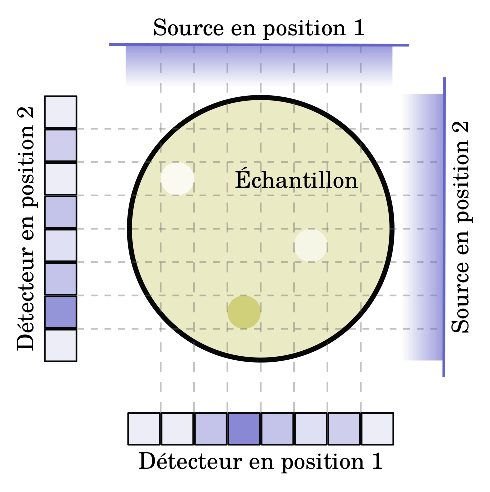
\includegraphics[]{principe_tomo.eps}
				\caption{\label{fig03:principe_tomo}Mise en évidence de la méthode de tomographie sur une coupe transversale d'un échantillon cylindrique : l'échantillon (ou l'appareillage) tourne sur l'axe normal au plan de la coupe de manière à prendre plusieurs radiographies.}
			\end{figure}
			\begin{figure}\centering
				\subfloat[]{
					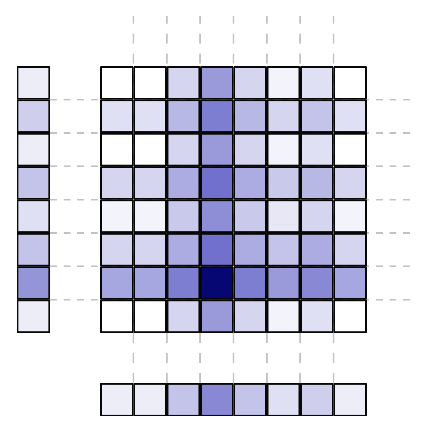
\includegraphics[]{reconstruction_tomo_00.eps}}\hspace{1cm}
				\subfloat[]{
					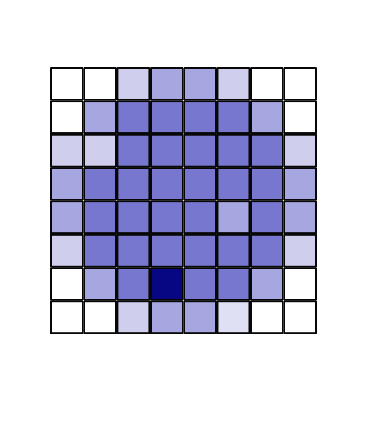
\includegraphics[]{reconstruction_tomo_01.eps}}
				\caption{\label{fig03:reconstruction_tomo}Méthode de reconstruction des images par superposition des radiographies : (a) résultat obtenu avec 2 positions différentes (cas de la figure \ref{fig03:principe_tomo}) et (b) avec un nombre bien plus grand de projections.}
			\end{figure}
			\\La reconstruction en tomographie, obtenue par superposition des projections, donne un champ scalaire tri-dimensionnel correspondant au champ d'absorption des rayons X dans l'espace. Tout comme un champ scalaire à deux dimensions peut être perçu comme une image dont chaque pixel correspond à un scalaire, le fichier de sortie de la tomographie peut se mettre sous la forme d'une image en trois dimensions où chaque voxel correspond à un scalaire. Il est alors possible de travailler sur ces images pour les améliorer et les analyser, c'est ce que nous allons voir dans le paragraphe suivant.
	\subsection{Traitements d'images 3D}\label{para03:traitement_image}
		Cette partie s'intéresse aux procédés numériques permettant de modifier les volumes donnés par la tomographie. Le lecteur peut se référer à \citet{bovik_handbook_2010} afin de mieux comprendre les processus de traitements d'images décrits dans la suite. Que ce soit en 2D ou en 3D, toute image est définie par un format déterminant la taille de l'image en fonction de ses dimensions. Nous ne considérerons que des images monochromatiques, donc ayant un seul canal (en niveaux de gris), de manière à ce que chaque pixel/voxel soit associé à un seul scalaire. L'élément unitaire constituant l'image sera dès à présent appelé voxel puisqu'une généralité pourra être faite aux images 3D. Le format s'exprime en "bit" et indique les valeurs qu'un voxel peut prendre. Par exemple, les voxels d'une image au format 8-bit ne peuvent prendre que $2^8$ soit $256$ valeurs : l'image sera constituée de voxels ayant des valeurs comprises entre 0 et 255 et dont la taille en mémoire vaut 1 octet. Une image 2D au format 16-bit (donc $2$ octets) de dimension $900\times 700$ aura des valeurs comprises entre $0$ et $2^{16}-1=65535$ et aura une taille en mémoire de $900\times 700\times 2=1260000$ octets. Les images issues de la tomographie et traitées dans cette thèse sont des images au format 8-bit en niveaux de gris. Elle pourraient être sauvegardées sous forme de matrices à trois dimensions directement lues par un langage de programmation ou un éditeur de texte mais cela ne s'avère pas pratique pour la visualisation. Généralement, les images 3D sont sauvegardées en couches, que l'on appelle aussi "stacks". En effet, les voxels étant orientés selon un repère orthonormal à trois dimensions, il est possible d'enregistrer les images en 2D (couche de 1 voxel) pour chaque couche normales à une direction du repère. Par exemple, une image de taille $M\times N\times H$ peut s'enregistrer sous forme de $H$ images de taille $M\times N$. Le visualisation se fait alors couche par couche de manière à pouvoir observer l'intégralité de l'échantillon.
		\\Un outil très utile en traitement et analyse d'images est l'histogramme. Il s'agit d'un type de graphe, souvent sous forme de barres verticales, qui indique pour chaque valeur d'intensité de voxel possible (en fonction du format de l'image) le nombre de voxels ayant cette valeur.
		\subsubsection{Binarisation par Seuillage}\label{para03:threshold}
			Les images en niveau de gris ont l'avantage de fournir plus ou moins d'information concernant le niveau d'absorption des rayons X au sein de l'échantillon. Cependant, pour de nombreuses tâches de post-traitement et d'analyse, cette information ne s'avère pas toujours utile. En effet, dans de nombreux cas il est utile de connaître uniquement les phases en présence. Ainsi, si l'échantillon est constitué de deux phases, ce que nous considérerons dans la suite, alors uniquement deux valeurs sont nécessaires pour définir l'image. Ces deux valeur peuvent par exemple être $0$ pour la phase constituant le vide (donc les pores) et $255$ pour la matière constituant les grains. Lorsque le matériau est biphasique il y a un autre avantage : on peut choisir de travailler sur des images binaires très légères au format "1-bit" prenant les valeurs $0$ ou $1$.
			\\Une méthode qui consiste à transformer une image quelconque en image binaire est une méthode de binarisation et se fait généralement par seuillage. Le seuillage consiste à déterminer une valeur seuil pour laquelle les voxels dont la valeur est inférieure prennent la première valeur binaire tandis que ceux dont la valeur est supérieure prennent l'autre valeur binaire. La détermination de cette valeur seuil peut se faire selon différentes méthodes, automatiques ou non.
			\\La méthode de binarisation la plus simple consiste à visualiser l'image binaire après chaque seuillage de manière à choisir, au choix de l'utilisateur, la valeur de seuil la plus cohérente avec le résultat attendu. Cette méthode est simple mais peut s'avérer également longue lorsque de nombreuses images sont à traiter. De plus, cette méthode est très dépendante de l'utilisateur. Afin de palier à ces problèmes, il existe plusieurs méthodes automatiques : ces dernières, bien qu'étant plus complexes d'un point de vue technique, sont très simples et très rapides à mettre en \oe{}uvre du point de vue de l'utilisateur et ne dépendent pas directement de l'utilisateur mais de l'allure de l'histogramme. Ces méthodes automatiques ont été employées et sont présentées au paragraphe \ref{para04:seuillage}.
		\subsubsection{Filtres binaires de bases}\label{para03:filtres}
			Toute personne ayant fait un minimum de traitement d'images a entendu parler de filtres. Un filtre est à l'image ce que l'opérateur algébrique est à la matrice - n'oublions pas qu'une image est une matrice. Cet opérateur numérique est capable de transformer l'image entièrement mais il est utilisé dans la très grande majorité des cas de manière itérative et sur des petites zones de l'image. Les zones de travail des filtres sont appelés noyaux ou éléments structurants et la taille de ces éléments ainsi que leur forme sont choisies par l'utilisateur. Chaque voxel de l'image se voit appliquer le filtre de la manière suivante : les voxels constituants le noyau par rapport au voxel en cours de traitement sont analysés afin de déterminer la nouvelle valeur de ce dernier. Le choix de la forme et de la taille de l'élément structurant aura un impact très fort sur le résultat, le nombre d'itération du filtre est également quelque chose d'important. Quelques filtres basiques, travaillant sur des images binaires (valeurs possibles : $0$ ou $1$, respectivement blanc et bleu sur la figure \ref{fig03:morpho_math}) vont être décrits ci-dessous :
			\begin{itemize}
				\item \'Erosion : s'il existe un voxel de l'élément structurant ayant la valeur $0$ (blanc) alors la valeur $0$ (blanc) est attribuée au voxel en cours d'analyse. Ce filtre donne plus d'importance aux voxels blancs proches des frontières entre les phases blanches et bleues. Si on considère les voxels $1$ (bleus) comme étant de la matière, alors ce filtre simule l'effet d'une érosion de la matière.
				\item Dilatation : il s'agit du filtre opposé à l'érosion. S'il existe dans le noyau un voxel de valeur $1$ (bleu) alors la valeur attribuée est $1$ (bleu). Cette fois-ci le filtre s'apparente à une dilatation de la matière.
				\item Ouverture : l'opération d'ouverture consiste à appliquer successivement une érosion puis une dilatation avec le même élément structurant. L'ouverture permet de supprimer les voxels bleus isolés dans les phases blanches.
				\item Fermeture : application successive d'une dilatation puis d'une érosion avec un même noyau. Il s'agit ici d'éliminer des petits groupes de voxels blancs isolés dans les phases bleues.
			\end{itemize}
			\begin{figure}\centering
				\subfloat[Image binaire d'origine]{
					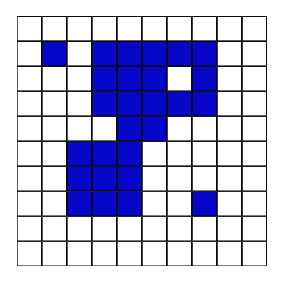
\includegraphics[scale=.8]{morpho_math_00.eps}}
				\subfloat[Noyau]{
					\hspace{1cm}
					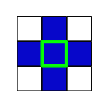
\includegraphics[scale=.8]{morpho_math_01.eps}
					\hspace{1cm}}\\
				\subfloat[\'Erosion]{
					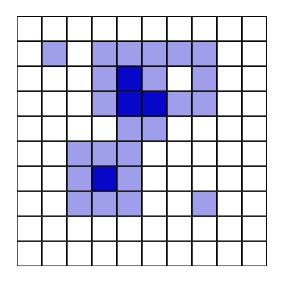
\includegraphics[scale=.8]{morpho_math_erosion.eps}}\hspace{3mm}
				\subfloat[Dilatation]{
					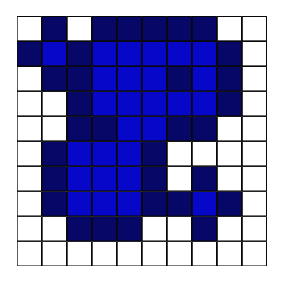
\includegraphics[scale=.8]{morpho_math_dilatation.eps}}\hspace{3mm}
				\subfloat[Ouverture]{
					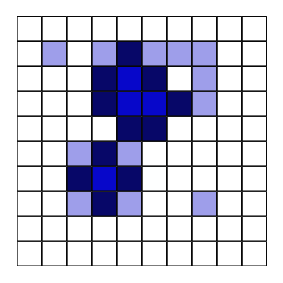
\includegraphics[scale=.8]{morpho_math_ouverture.eps}}\hspace{3mm}
				\subfloat[Fermeture]{
					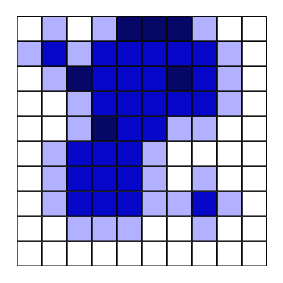
\includegraphics[scale=.8]{morpho_math_fermeture.eps}}
				\caption{\label{fig03:morpho_math}Effets des filtres morphologiques de base (c-f) sur une image binaire (a) en utilisant l'élément structurant (b). Les pixels en transparence sont ceux qui s'annulent (deviennent blancs), ceux qui apparaissent plus foncés sont ceux qui s'activent (deviennent bleus).}
			\end{figure}
			Les explications concernant ces filtres peuvent être trouvées dans les lectures de \citeauthor{heijmans_algebraic_1990} \citep{heijmans_algebraic_1990, ronse_algebraic_1991}. Ces filtres ne sont pas destinés uniquement aux images binaires puisqu'ils fonctionnent également sur des images en niveaux de gris. Une illustration des effets du filtre est présentée sur la figure \ref{fig03:morpho_math}.

		\subsubsection{Segmentation}
			La segmentation est le processus de reconnaissance du signal pour attribuer une identité, un label, à chaque partie du signal. C'est par un processus de segmentation qu'un code informatique est capable de reconnaître la morphologie ou l'intensité d'une certaine entité dans une image. Il existe de nombreuses méthodes de segmentation qui considèrent l'image comme une carte topologique et simulent des phénomènes naturels pour engendrer des structures géodésiques. De nombreux ouvrages destinés à la morphologie mathématique expliquent ces méthodes (\citet{haralick_image_1987} et \citet{dougherty_mathematical_1992} en sont des exemples).
			\\L'algorithme utilisé dans cette thèse est régulièrement utilisé pour la segmentation. Il s'agit de la méthode du "watershed" qui est illustrée sur la figure \ref{fig03:watershed}. Avec cette méthode, l'intensité des voxels peut être comparée à une altitude, les zones d'identification des grains à des lacs et la propagation de ces zones à une montée des eaux. Lorsque plusieurs lacs sont présents sur un profil altimétrique et qu'une montée des eaux se réalise, les lacs augmentent en taille en même temps qu'ils gagnent de l'altitude. Lorsque deux lacs se rejoignent au niveau d'un sommet alors une ligne de partage des eaux apparaît : c'est à cet endroit qu'une digue sera construite si le mélange des eaux n'est pas souhaité. Lorsque l'eau arrive sur un sommet mais que l'autre côté du sommet n'est pas immergé alors l'eau se propagera automatiquement de l'autre côté du sommet. Ce phénomène continue jusqu'à ce que la montée des eaux se termine.
			La méthode de segmentation par watershed fonctionne de manière identique. Dans une zone d'appartenance certaine à un grain, un marqueur est créé afin d'identifier ce grain (un lac est créé). Ce processus est réalisé pour chacun des grains dans la limite du possible. Chaque marqueur est unique : il en existe un seul par grain. Maintenant que chaque grain est identifié et existe, il est nécessaire de propager les marqueurs dans l'image afin qu'ils prennent la forme de chacun des grains (montée des eaux). La propagation est réalisée en fonction du champ d'intensité des voxels (profil altimétrique) : les voxels qui touchent les marqueurs et qui ont une intensité inférieure ou égale à celle du marqueur prennent la valeur du marqueur (inondation), ceux qui ont une intensité directement supérieure ne seront immergés que dans l'étape suivante. Lorsque deux marqueurs se rejoignent, ils restent indépendants et le processus peut continuer (création d'une digue). Le processus continue jusqu'à ce que les marqueurs atteignent une intensité définie comme valeur seuil d'appartenance aux grains.
			\begin{figure}\centering
				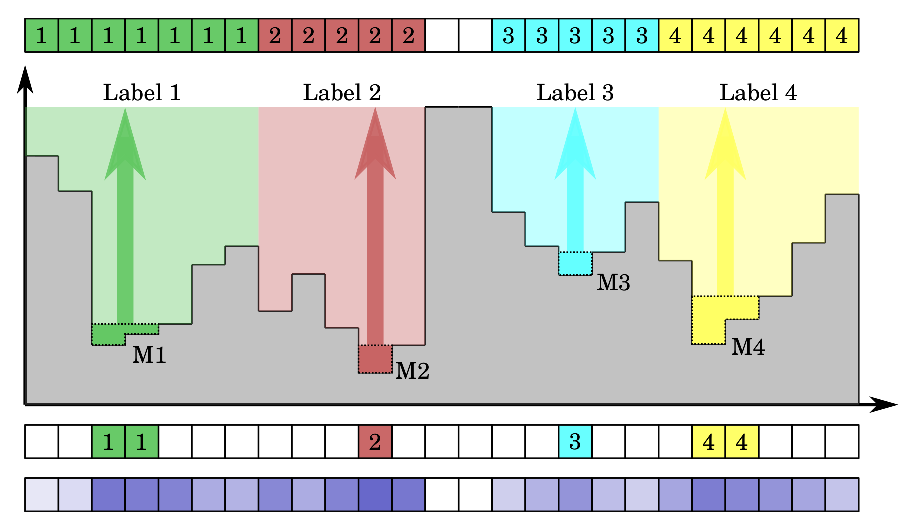
\includegraphics[]{watershed.eps}
				\caption{\label{fig03:watershed}Principe de segmentation par watershed (de bas en haut): signal sur une dimension ; masque des marqueurs (de même dimension que l'image) ; analogie géodésique : le signal donne l'altitude et les marqueurs sont des lacs, puis montée des eaux ; signal segmenté.}
			\end{figure}
	\subsection{Corrélation d'images numériques 3D}\label{para03:DIC}
		La corrélation d'images numériques (DIC pour Digital Image Correlation) est un outil puissant pour les mécaniciens puisqu'il permet de mesurer un champ cinématique hétérogène lors d'essais expérimentaux. Lors des essais, des photographies de l'échantillon sont prises au cours du temps de manière à observer les déplacements en surface d'échantillon en comparant les photographies. On voit de suite l'intérêt de la tomographie dans ce domaine : il est alors possible d'observer les déplacements dans un volume plutôt que dans un plan. On parle alors de corrélation de volumes numériques (DVC pour Digital Volume Correlation).
		\\Le principe de la corrélation d'images, qu'elles soient 2D ou 3D, se base sur la comparaison de deux images. Pour cela il est nécessaire de définir le coefficient de corrélation normalisé CCN qui est calculé pour comparer deux images $I_1$ et $I_2$:
		\begin{equation}\label{eq03:NCC}
			\mathrm{CCN} = \cfrac{\sum_{x,y,z} \left(I_1(x,y,z)\cdot I_2(x+u, y+v, z+w)\right)}{\sqrt{\sum_{x,y,z} I_1(x,y,z)\cdot \sum_{x,y,z} I_2(x+u, y+v, z+w)}}
		\end{equation}
		où $I_1(x,y,z)$ est la valeur en niveaux de gris du voxel de l'image de référence situé aux coordonnées $x$, $y$ et $z$ et $I_2$ est l'image à comparer, déplacée de $u$ suivant $x$, $v$ suivant $y$ et $w$ suivant $z$. Plus la valeur de ce coefficient à une valeur proche de $1$, plus la similarité entre les deux images est grande. Si $I_1$ et $I_2$ partagent exactement le même signal alors le coefficient de corrélation normalisé vaudra $1$.
		\\La mesure des champs de déplacements est basée sur la corrélation d'images. En effet, si on divise l'image d'origine en plusieurs images, plus petites, appelées "imagettes" et que l'on définit des zones de recherche des mêmes imagettes dans l'image à comparer alors il existe pour chaque zone de recherche un triplet $(u,v,w)$ qui maximise le coefficient de corrélation normalisé. Si ce coefficient maximal est proche de $1$ alors il est supposé que le déplacement subit par l'imagette est de $u$ voxels dans la direction $(Ox)$, $v$ voxels dans la direction $(Oy)$ et $w$ voxels dans la direction $(Oz)$. La connaissance de la taille des voxels indique la mesure réelle.
		\\Il est à noter que :
		\begin{itemize}
			\item Une image non contrastée et uniforme ne permettra pas de trouver un maximum pour CCN dans la zone de recherche puisque les signaux $I_1$ et $I_2$ seront quasi-identiques partout. Il faut des hétérogénéités, qu'elles soient naturelles ou artificielles.
			\item Plus les imagettes sont petites, meilleure est la résolution du champ de déplacement.
			\item La taille des imagettes dépend de la taille des hétérogénéités dans l'échantillon.
			\item Pour obtenir plus de précision concernant la mesure des déplacements, il est nécessaire de faire une interpolation 3D sur le volume. De base, la précision de la mesure est de l'ordre de la taille du voxel. Si on augmente le nombre de voxels alors la précision est également augmentée (au prix d'un calcul plus lourd).
			\item La corrélation ne peut se faire qu'entre deux imagettes quasi-identiques. Si la déformation de l'imagette entre l'image de référence et l'image à comparer est trop grande alors la corrélation sera mauvaise et le déplacement inconnu. Pour visualiser les déplacements sur des échantillons grandement déformés il est nécessaire de mesurer et sommer les déplacements sur des états successifs relativement proches (\textit{i.e.} pour des états dont la déformation n'évolue que faiblement).
		\end{itemize}
		Il existe d'autres types de mesures de corrélation mais celle présentée ici est sans nul doute la plus utilisée. De la même manière, il existe plusieurs méthodes algorithmiques permettant de mesurer les champs de déplacements. Le choix a été fait de se concentrer sur la méthode utilisée dans les travaux de cette thèse. Il est d'ailleurs utile de préciser que le code Tomowarp2 a été utilisé afin de mener les calculs de corrélation sur les images de tomographie. Une description de ce code est donnée par \citet{tudisco_tomowarp2_2017}.

\section{Simulations numériques des milieux granulaires}\label{para:methodes_simu}
	Les outils numériques permettent aux mécaniciens actuels de réduire significativement les campagnes d'essais grâce aux simulations numériques. Il est par exemple possible de mener dans le même temps plusieurs essais dont seuls quelques paramètres changent afin d'en étudier leur effet. Afin de s'assurer de la pertinence des résultats issus des simulations numériques, il est primordial que l'utilisateur du programme connaisse la méthode de simulation utilisée. En effet, il est nécessaire de savoir de quelle manière est discrétisée la géométrie de l'échantillon numérique, de quelle manière peuvent être attribuées les conditions aux limites, de quelle manière la loi de comportement des éléments a été créée ou encore de quelle manière les itérations de calculs sont définies.
	\\Globalement, les méthodes de simulation sont basées sur la discrétisation de la géométrie. Ainsi, un matériau réel qui est défini de manière continue sera approximé par un matériau dont les propriétés sont définies sur un certain nombre d'éléments. Nous allons, dans cette partie, nous concentrer sur des méthodes très utilisées en simulations mécaniques : les éléments discrets et les éléments finis.
	\subsection{Méthode des éléments discrets (DEM)}
		\subsubsection{Description de la méthode}
			La méthode des éléments discrets (DEM pour Discrete Element Method/Model) est une méthode qui a commencé à être réellement développée dans les années 1980 \citep{cundall_discrete_1979} mais qui s'est grandement popularisée à partir du milieu des années 1990. Il s'agit d'une méthode adaptée à la modélisation des milieux granulaires puisque les éléments discrets sont les particules constituant le milieu granulaire. Il y a donc autant d'éléments géométriques dans la simulation que de grains dans l'échantillon simulé. La DEM s'est construite essentiellement à partir de simulations faites sur les structures moléculaires. Les structures moléculaires étant constituées d'atomes, il est possible de les modéliser par un ensemble de sphères ayant un certain arrangement. Cet arrangement dépend de l'environnement puisque des forces interatomiques existent. La dynamique des sphères est donc très dépendante de cet environnement et il est possible de simuler le comportement d'un tel milieu grâce à ce qu'on appelle la dynamique moléculaire. Il existe cependant des différences considérables entre le modèle moléculaire et un milieu granulaire. En effet, les particules macroscopiques sont soumises à de la friction solide et engendre des interactions entre particules différentes des interactions entre atomes, qui eux, subissent des forces normales dérivant de potentiels.
			\\On distingue différentes méthodes parmi les méthodes DEM \citep{cambou_micromechanics_2009}, entre autre :
			\begin{itemize}
				\item les méthodes \emph{smooth DEM} pour lesquelles les interactions intergranulaires sont décrites par des fonctions continues et suffisamment différentiables. Les méthodes de dynamique moléculaire décrites plus haut font parties de la smooth DEM. \citet{cundall_discrete_1979} a également exposé des travaux réalisés avec cette méthode en utilisant des systèmes de ressorts et d'amortisseurs pour décrire les forces d'interaction de contact.
				\item les méthodes \emph{non smooth DEM} pour lesquelles les interactions intergranulaires sont décrites par des lois de choc ou toute autre relation décrivant les sauts de vitesse et les seuils de force. L'approche la plus utilisée est sans doute celle des contacts dynamiques développée par \citet{moreau_unilateral_1988} et \citet{jean_unilaterality_1992}.
			\end{itemize}
			La liste qui précède n'est pas une liste exhaustive des méthodes de simulation par DEM. Le lecteur pourra aisément s'informer sur d'autres méthodes \citep{bardet_introduction_1998}, mais également mieux connaître les différences entre les méthodes "smooth" et "non smooth" en se rapportant à la lecture de \citet{wolf_modelling_1996}.
			\\La figure \ref{fig03:principe_DEM} illustre le principe de la simulation par éléments discrets.
			\begin{figure}\centering
				\begin{tikzpicture}
					\tikzset{court/.style={draw, rectangle, rounded corners=3pt},
							 long/.style={draw, rectangle, rounded corners=3pt, text centered}}
					\draw[->, >=latex, very thick] (0,1) arc (80:-260:1);
					\node[above] (increment) at (0,1) {$+\Delta t$};
					\node[court, above right] (contacts) at (38:1.05) {Détection des contacts};
					\node[long, right, text width=6cm] (forces) at (-15:1.05) {Calcul des forces de contact (normales et tangentielles)};
					\node[long, below, text width=6cm] (total) at (-90:1.2) {Calcul de la force totale appliquée à chaque particule};
					\node[long, left, text width=5cm] (accelerations) at (-167:1.4) {Calcul des accélérations liées aux forces};
					\node[long, above left, text width=5cm] (nouveau) at (150:1.25) {Nouvelles positions et vitesses des particules};
				\end{tikzpicture}
				\caption{\label{fig03:principe_DEM}Méthode de simulation par éléments discrets}
			\end{figure}
		\subsubsection{Matériaux et géométries employés}
			Le principal objectif de la méthode des éléments discrets et de pouvoir simuler un milieu granulaire suffisamment volumineux pour connaître la réponse mécanique du milieu à l'échelle macroscopique. En ayant connaissance du nombre de particules nécessaires pour décrire le comportement d'un milieu granulaire, on s'aperçoit vite des limitations liées aux outils numériques. Il faut pouvoir modéliser un très grand nombre de particules, ayant chacune plusieurs degrés de liberté et plusieurs contacts. Pour cette raison, la très grande majorité des simulations sont réalisées sur des collections de grains de formes relativement simples et régulières (disques, sphères, polyèdres réguliers) afin de modéliser les grains par un minimum de points représentatifs.
			\\De par la nature indéformable des éléments discrets, la méthode DEM est largement utilisée dans les problèmes d'écoulements granulaires, pour lesquels la déformation physique des grains est négligeable \citep{vu-quoc_accurate_1999, vu-quoc_normal_2001, wu_experimental_2003}. Cependant, en utilisant un loi de contact adaptée, la méthode montre également son utilité dans l'étude de la densification des matériaux granulaires comme le montre les travaux de \citet{heyliger_cold_2001, martin_study_2003, martin_study_2003-1, skrinjar_discrete_2004} au début des années 2000.
		\subsubsection{Limites de la méthode}
			Les simulations par DEM ont leurs avantages mais présentent également une limite majeure pour l'étude des grains déformables. En effet, une fois fixée au départ de la simulation, la géométrie des grains reste la même durant la simulation. Malgré les méthodes mises en place pour modéliser la déformation des grains en DEM, le changement de forme des particules n'est pas pris en compte. De cette manière, pour un matériau granulaire dont les grains sont déformables, et pour de grandes déformations des grains, la réponse mécanique réelle du milieu peut être assez différente de la simulation.
	\subsection{Méthode des éléments finis (FEM)}
		\subsubsection{Description de la méthode}
			La méthode des éléments finis (FEM pour Finite Element Method) est une méthode couramment utilisée en calcul des structures pour la conception et le dimensionnement. La méthode n'est pas uniquement dédiée aux structures puisqu'elle est capable de résoudre un large éventail de problèmes : structurels, thermiques, électromagnétiques, fluidiques, en linéaire, en non linéaire, en stationnaire ou en transitoire. On voit ici la puissance de la méthode et on comprend l'intérêt des ingénieurs et chercheurs dans l'utilisation d'outils utilisant cette méthode. La méthode a commencé à se développer dans les années 1940 avec les travaux de \citet{hrennikoff_solution_1941} et \citet{courant_variational_1943}. Le principe de base de la méthode FEM consiste à discrétiser un milieu continu en un ensemble d'éléments de géométrie connue et dont les propriétés sont définies en amont de la simulation. La génération d'un maillage adapté est nécessaire pour modéliser au mieux une structure continue en un nombre fini d'éléments. Chaque point singulier d'un élément fini est appelé n\oe{}ud. Ce sont les n\oe{}uds qui possèdent un certain nombre de degrés de liberté et permettent à la structure de se mouvoir sous l'action de forces. Une des méthode de résolution couramment utilisée est celle de Rayleigh-Ritz et consiste à minimiser l'énergie potentielle du système en la décrivant comme la différence entre l'énergie de déformation et le travail des forces volumiques et/ou surfaciques. Cette minimisation de l'énergie donne généralement une équation de la forme :
			\begin{equation}\label{eq03:equation_FEM}
				[K]\cdot \{Q\} - \{F\} = 0 \qquad \Leftrightarrow \qquad [K]\cdot \{Q\} = \{F\}
			\end{equation}
			où $[K]$ est la matrice raideur, $\{Q\}$ est le vecteur donnant les différents degrés de liberté et $\{F\}$ est le vecteur des forces appliquées aux n\oe{}uds. Avec cette équation, pour chaque n\oe{}ud, il est possible de connaître la force appliquée (ou résultante) et le déplacement imposé (ou résultant). On obtient ainsi des champs de force et de déplacement plus ou moins proches des champs réels en faisant une interpolation sur chaque élément fini.
			\\La méthode de simulation par éléments finis est décrite sur la figure \ref{fig03:methode_FEM}. Une première étape consiste à calculer la matrices de raideur et le vecteur de charges pour chaque élément du maillage dans les repères locaux. Ensuite, une nouvelle boucle est faite sur les éléments du maillage afin de déterminer la matrice de passage entre le repère local et le repère global ; à partir de cette matrice de passage, la matrice de raideur et le vecteur de charge sont exprimées dans le repère global. Une matrice d'assemblage est ensuite créée de manière à reconstruire les matrices et vecteurs du système dans son intégralité (avec tous les degrés de liberté). L'équation (\ref{eq03:equation_FEM}) peut finalement être résolue de manière à connaître les forces et déplacements en tout n\oe{}ud de la structure maillée et les efforts internes peuvent être calculés. Si le lecteur s'intéresse plus particulièrement à la méthode FEM, il peut se reporter à la lecture de \citet{cazenave_methode_2013}.
			\begin{figure}\centering
				\begin{tikzpicture}
					\tikzset{etape/.style={draw, rectangle, below, rounded corners=3pt, text centered}}
					\tikzset{long/.style={draw, rectangle, below, rounded corners=3pt, text width=8cm, text centered}}
					\tikzset{fleche/.style={->, >=latex, thick}}
					\tikzset{increment/.style={rotate=90}}
					\tikzset{explication/.style={above, text width=4cm, text centered, rotate=-90, shift={(0,5.2)}}}
					\node[etape] (Structure)at(0,0){Structure à $n$ n\oe{}uds et $m$ éléments};
					\node[etape, shift={(0,-.6)}] (Init1)at(Structure.south){$e=1$};
					\node[long, shift={(0,-.6)}] (local1)at(Init1.south){Construction de la matrice de rigidité $[k_e]$ (repère local)};
					\node[long, shift={(0,-0.6)}] (local2)at(local1.south){Construction du vecteur de charges $\{f_e\}$ (repère local)};
					\node[etape, shift={(0,-0.6)}] (Init2)at(local2.south){$e=1$};
					\node[long, shift={(0,-0.6)}] (global1)at(Init2.south){Calcul de la matrice de passage $[R_e]$ liant repères global et local};
					\node[long, shift={(0,-0.6)}] (global2)at(global1.south){Calcul de la matrice de rigidité dans le repère global $[K_e]=[R_e]^T\cdot [k_e]\cdot [R_e]$};
					\node[long, shift={(0,-0.6)}] (global3)at(global2.south){Calcul du vecteur charges dans le repère global $\{F_e\}=[R_e]^T\cdot \{f_e\}$};
					\node[long, shift={(0,-0.6)}] (assemblage1)at(global3.south){Assemblage de $[K]$};
					\node[long, shift={(0,-0.6)}] (assemblage2)at(assemblage1.south){Assemblage de \{F\} en tenant compte des charges nodales};
					\node[long, shift={(0,-0.6)}] (resolution)at(assemblage2.south){Résolution du système $\{F\}=[K]\cdot \{Q\}$ après introduction des conditions d'appui};
					\node[etape, shift={(0,-0.6)}] (Init3)at(resolution.south){$e=1$};
					\node[long, shift={(0,-0.6)}] (interne)at(Init3.south){Calcul des efforts internes en repère local $[k_e]\cdot\{q_e\}$};
					\node[etape, shift={(0,-0.6)}] (fin)at(interne.south){Fin};
					\node[increment, shift={(-.3,5)}] (iter1)at(local1.south){$m$ élements};
					\node[increment, shift={(0,5)}] (iter2)at(global2.center){$m$ élements};
					\node[increment, shift={(0,5)}] (iter3)at(interne.center){$m$ élements};
					\node[shift={(0,-.3)}] (iter1haut)at(Init1.south){}; \node[shift={(0,-.3)}] (iter1bas)at(local2.south){};
					\node[shift={(0,-.3)}] (iter2haut)at(Init2.south){}; \node[shift={(0,-.3)}] (iter2bas)at(global3.south){};
					\node[shift={(0,-.3)}] (iter3haut)at(Init3.south){}; \node[shift={(0,-.3)}] (iter3bas)at(interne.south){};
					\draw[fleche] (Structure) -- (Init1); \draw[fleche] (Init1) -- (local1); \draw[fleche] (local1) -- (local2);
					\draw[fleche] (local2) -- (Init2); \draw[fleche] (Init2) -- (global1); \draw[fleche] (global1) -- (global2);
					\draw[fleche] (global2) -- (global3); \draw[fleche] (global3) -- (assemblage1);
					\draw[fleche] (assemblage1) -- (assemblage2); \draw[fleche] (assemblage2) -- (resolution);
					\draw[fleche] (resolution) -- (Init3); \draw[fleche] (Init3) -- (interne); \draw[fleche] (interne) -- (fin);
					\draw[fleche] (iter1bas) -| (iter1) |- (iter1haut);
					\draw[fleche] (iter2bas) -| (iter2) |- (iter2haut);
					\draw[thick] (iter3bas) -- ++(-4.7,0); \draw[<-, >=latex, thick] (iter3haut) -- ++(-4.7,0);
					\node[explication] (expl2) at (global2.center) {Passage du repère local au repère global};
					\node[explication, shift={(-.3,0)}] (expl1) at (local2.north) {Calculs dans le repère local};
					\node[above, text width=8cm, text centered, rotate=-90, shift={(0,5.2)}] (expl3) at (resolution.center) {Assemblage des matrices élementaires, résolution puis calculs des efforts internes};
				\end{tikzpicture}
				\caption{\label{fig03:methode_FEM}Organigramme générale de résolution par la méthode FEM (cas d'un calcul en statique) \citep{cazenave_methode_2013}}
			\end{figure}
		\subsubsection{Matériaux et géométries employés}
			La méthode des éléments finis est une méthode de simulation utilisée pour les structures continues. En effet, le principe de la méthode FEM est d'approximer au mieux le comportement d'un milieu continu en le discrétisant. Les champs en sortie de simulation sont interpolés de manière à obtenir des champs continus. La génération d'un maillage approprié est indispensable pour rendre la méthode efficace. Plus les éléments du maillage seront petits, plus longs seront les temps de calculs mais meilleure sera la solution puisque l'approximation se rapproche alors du modèle continu. En plus de la densité du maillage, le choix des éléments constituant le maillage est important. C'est en effet en fonction de leur géométrie et de leurs propriétés qu'il est possible de simuler certains comportements avec une plus ou moins grande précision.
			\\Les progrès réalisé en informatique ces dernière décennies (puissance de calculs et interactions homme/machine notamment) ont permis d'évoluer vers des méthodes sophistiquées qui ne s'arrêtent plus aux cas de la statique linéaire. De nombreux bureaux d'études travaillent aujourd’hui sur des problèmes de statique non linéaire et même de dynamique non linéaire.
		\subsubsection{Limites de la méthode}
			De très nombreux calculs sont nécessaires pour résoudre un problème de calcul de structure par éléments finis. En fonction de la méthode utilisée, à chaque élément du maillage est associé un certain nombre de vecteurs et matrices qui doivent être calculés et assemblés dans des vecteurs ou matrices bien plus grands dont la taille dépend du nombre de degrés de liberté du problème. Cela se passe à chaque incrément de temps pour des calculs en dynamique ou quasi-statique. Pour cette raison, les simulations de structures complexes - nécessitant donc un maillage fin - subissant de larges déformations vont demander une très grande puissance de calcul et de stockage informatique. Il est donc important de savoir optimiser la méthode à partir d'hypothèses fondées (définition d'un incrément de temps, choix de la densité du maillage, etc.).
			\\Une étape indispensable à la méthode des éléments finis est celle de la génération du maillage qui n'est pas toujours évidente et pose souvent des problèmes aux ingénieurs en bureaux d'études. En effet, il est primordial de savoir choisir le type d'élément définissant le maillage en fonction des simulations et de savoir gérer, dans le même temps, la densité du maillage. Certaines parties de la géométrie des structures modélisées peuvent nécessiter un maillage très fin alors que la plus grande partie de cette structure peut être définie par un maillage assez grossier. Dans ce cas, le travail technique consiste à faire un maillage qui prend en compte de nombreux facteurs. Ces facteurs peuvent être plus ou moins bien connus et pondérés par un logiciel informatique mais c'est souvent l'expérience et les connaissances du technicien sur le modèle qui vont permettre de générer un maillage approprié. La méthode FEM est donc très dépendante de l'utilisateur.
	\subsection{Méthode des éléments finis multi-particules (MP-FEM)}
		\label{para03:MPFEM}
		\subsubsection{Description de la méthode}
			La méthode des éléments finis multi-particules (MP-FEM pour Multi-Particules Finite Element Method) est basée sur la méthode FEM mais s'intéresse également aux interactions existantes entre différentes particules de la même manière qu'avec la méthode DEM. Les travaux de \citet{ransing_powder_2000}, \citeauthor{gethin_numerical_2001} \citep{gethin_numerical_2001, gethin_two_2006} et \citet{lewis_combined_2005} réalisés au début des années 2000 font partie des premiers travaux utilisant cette méthode sur des matériaux granulaires déformables. Toutefois, les simulations concernées par ces premiers travaux étaient en 2D. Depuis, la méthode MP-FEM n'a cessé de se développer grâce aux travaux de \citet{procopio_simulation_2005} et aux premières simulations 3D apparues en 2007 avec les travaux de \citet{chen_numerical_2007} et \citeauthor{frenning_efficient_2008} \citep{frenning_efficient_2008, frenning_compression_2010}. Peu d'années après, \citet{schmidt_simulation_2010} et \citet{harthong_study_2012} utilisent les éléments finis pour étudier la plasticité des grains par l'obtention des surfaces de charge. \citet{gustafsson_multi_2013} va même jusqu'à reproduire les phénomènes de fissuration lors de la compression de particules de minerai de fer. Plus récemment, la méthode a été utilisée par \citeauthor{guner_numerical_2015} \citep{guner_numerical_2015, guner_effects_2018} afin d'étudier la compaction d'une poudre de cuivre et de mieux comprendre les effets des paramètres de compression (vitesse de chargement, lubrification, température). \citet{loidolt_modeling_2018} a, quant à lui, utilisée la méthode MP-FEM dans le but d'observer l'effet des forces de contact cohésives entre les grains sur la surface de charge. \citet{feng_cohesive_2019} couple la MP-FEM avec la méthode de zone cohésive afin de simuler les fissuration dans des grains d'aluminium et de chlorure de sodium.
			\\Le principe de la méthode repose sur les principes des éléments discrets et des éléments finis. La figure \ref{fig03:DEM_MPFEM} illustre la manière dont est discrétisé un milieu granulaire avec la méthode MP-FEM (schéma de droite) comparée à celle de la méthode DEM (schéma de gauche). La discrétisation de la matière se fait par l'intermédiaire d'éléments finis. Ainsi, chaque particule est définie de la même manière qu'une structure dans un modèle éléments finis. La différence avec la méthode FEM intervient lorsqu'un assemblage de particules et d'interactions entre elles est créé de la même manière qu'avec la méthode DEM. En effet, des lois de contact sont définies entre les différents matériaux et sont appliquées lorsqu'un contact entre particules a été détecté.
			\\La méthode MP-FEM permet d'analyser la compression d'un empilement de grains sous des conditions de chargement quasi-statiques. L'expérience montre que l'utilisation d'un schéma d'intégration explicite dans le code commercial utilisé permet une convergence des simulations numériques d'empilements avec de nombreux contacts et de grandes déformations des particules. Ce schéma d'intégration n'exclut aucunement les erreurs de calcul et, pour cette raison, une comparaison des résultats numériques et expérimentaux est nécessaire. Cette méthode a l'avantage de prendre en compte l'évolution de la géométrie des particules au cours de la simulation et de fournir de nombreuses informations à l'intérieur des particules (champs de contraintes et de déformations notamment).
			\\Afin de valider la méthode MP-FEM, \citeauthor{chen_contribution_2008} \cite{chen_contribution_2008} a mené une campagne d'essais expérimentaux et numériques sur la compression de particules de plomb. La méthode de validation est basée sur la comparaison des résultats numériques et expérimentaux. Pour cela, l'auteur a comprimé un certain nombre de particules (seules ou dans un ensemble de particules) dans une presse hydraulique puis a mené des simulations numériques, avec la méthode MP-FEM, sur des géométries similaires à celles de l'expérimentation, avec des conditions de chargement identiques et une loi de comportement associée au matériau plomb. La comparaison des résultats expérimentaux et numériques montre l'efficacité de la méthode dans la simulation de la compression d'un empilement de particules très déformables. Cette efficacité a même été démontrée jusqu'à l'obtention d'un milieu dont la densité relative atteint \num{0.92} (la densité relative initiale étant proche de \num{0.60}).
			\begin{figure}\centering
				\includegraphics[width=0.8\textwidth]{DEM_MPFEM.png}
				\caption{\label{fig03:DEM_MPFEM}Illustration 2D des méthodes DEM (à gauche) et MP-FEM (à droite). Les éléments discrets sont indéformables et l'étude des contacts en surface des éléments, avec une loi de contact adaptée, est utilisée. Les éléments finis sont déformables, les champs de déformations et contraintes sont connus au sein des grains et les contacts en surface sont pris en compte avec une loi de contact adaptée. Illustration issue des travaux de thèse de \citet{harthong_modelisation_2010}.}
			\end{figure}
		\subsubsection{Matériaux et géométries employés}
			Par définition, tout comme la méthode des éléments discrets, la méthode MP-FEM est adaptée aux milieux granulaires. Le fait de générer un maillage pour chaque particule permet d'utiliser une bibliothèque de grains très diversifiée. Il est ainsi possible de modéliser le milieu granulaire avec des grains dont la géométrie est assez complexe et évolue au cours de temps.
		\subsubsection{Limites de la méthode}
			Bien que la possibilité de simuler un matériau granulaire avec des grains dont la géométrie est complexe soit un avantage de la méthode des éléments finis multi-particules, cette méthode hérite également des limites de la méthode des éléments finis. En effet, en fonction de la complexité des grains, un nombre plus ou moins important de n\oe{}uds va être nécessaire et, en fonction de la puissance de calcul disponible, le nombre de grains dans le milieu granulaire modélisé s'en retrouve limité. Pour une même puissance de calcul, une collection de grains pour la méthode MP-FEM sera généralement plus petite qu'une collection de grains pour la méthode des éléments discrets. En revanche, avec les éléments finis multi-particules, la déformation des grains est prise en compte dans le processus de simulation.
		
		\paragraph{}
		Il a été vu les nombreux avantages d'utiliser la méthode des éléments finis multi-particules dans le cadre de la simulation numérique de la compression des milieux granulaires dont les grains sont de nature déformable. Les moyens numériques ne cessent d'évoluer pour permettre des puissances de calculs toujours plus importantes et l'utilisation de mémoire toujours plus grande. Pour ces raisons, la méthode MP-FEM est vouée à être de plus en plus utilisée dans l'analyse de la compression des milieux granulaires. Cependant, les résultats actuels sur l'utilisation de cette méthode sont encore relativement pauvres comparé aux méthodes FEM et DEM. C'est la raison pour laquelle une méthode est développée dans cette thèse pour utiliser les éléments finis multi-particules sur une microstructure réelle afin de l'intégrer dans un code éléments finis et générer des simulations numériques pouvant être comparées directement aux essais expérimentaux.
		\\Quelques travaux basés sur une approche similaire ont été réalisés. En effet, l'utilisation de la tomographie pour intégrer une structure réelle dans une simulation par éléments finis a par exemple été observé dans les travaux de \citet{youssef_finite_2005} sur des matériaux cellulaires et \citet{wautier_linking_2015} sur la neige. \Citet{vlahinic2013} ont, quant à eux, menés des simulations DEM à partir d'informations obtenues par imagerie 3D. Cependant, au moment de la rédaction de ce manuscrit, l'auteur n'a pas connaissance de travaux pour lesquels les éléments finis multi-particules sont utilisés pour simuler le comportement mécanique d'un ensemble de particules déformables en interactions entre elles à partir des géométries réelles des particules et des conditions de chargement réellement observées par des méthodes d'imagerie 3D.
	\graphicspath{{./04-Experimentale/images/}}

\chapter{Travaux expérimentaux}
\label{chap:experimental}
	Le milieu granulaire qui est étudié dans les travaux de cette thèse est un milieu constitué de grains de polystyrène. Les particules ont une taille moyenne de \SI{150}{\micro\meter} et leurs formes sont très irrégulières. Le comportement du polystyrène est décrit dans le paragraphe \ref{para03:PS}.
	\\Afin d'analyser la réponse mécanique du milieu à des conditions de compression multiaxiales, l'essai de compression triaxiale de révolution a été choisi. Avec cet essai, le milieu granulaire va être confiné de manière isotrope puis, dans le même temps, un déplacement selon l'axe de l'échantillon est imposé de manière à engendrer une compression axiale. Le dispositif est instrumenté au moyen de capteurs de déplacement et de force dans le but de mesurer la déformation globale de l'échantillon et de connaître les efforts auxquels l'ensemble de grains est soumis.
	\\Dans le but d'obtenir des informations concernant la microstructure du milieu granulaire, une technique d'imagerie 3D est mise en \oe{}uvre. Ainsi, la tomographie à rayons X va permettre d'obtenir un champ de densité du milieu mais également des champs de déplacements et de déformations. L'obtention des déplacements et des déformations avec l'imagerie 3D est rendue possible grâce aux méthodes de corrélation de volumes numérique.

\section{Essais de compression triaxiale de révolution}
	L’essai de compression triaxiale de révolution suit un principe opératoire classique pour obtenir un mode de sollicitation homogène au sein de l’échantillon. A ce titre, un essai mené de manière idéale permet de ne suivre qu'un seul chemin de chargement. Compte tenu du fait que les travaux de cette thèse intègrent une approche par simulation numérique, la mise en \oe{}uvre d’un essai homogène est d’un grand intérêt pour observer des conditions aux limites proches entre expérimentation et simulation. Pour cette raison le protocole décrit ci-dessous montrera les étapes qui permettront de réaliser au mieux ce type d’essai.
	\subsection{Matériel et protocole expérimentale}
		Les essais de compression triaxiale (cf. paragraphe \ref{para03:triax}) ont été menés sur différents échantillons de poudre de polystyrène. La figure \ref{fig04:triax} rappelle le principe de la compression triaxiale. Bien que les essais aient des caractéristiques différentes, le protocole expérimental est toujours le même et respecte les étapes suivantes, illustrées par la figure \ref{fig04:deroulement_essai}.
		\begin{figure}\centering
			\includegraphics[scale=0.9]{../../03-Biblio/images/triax.eps}
			\caption{\label{fig04:triax}Principe de l'essai de compression triaxiale (cf. paragraphe \ref{para03:triax}).}
		\end{figure}
		\begin{figure}\centering
			\includegraphics[width=1.\textwidth]{deroulement_essai.png}
			\caption{\label{fig04:deroulement_essai}Les différentes étapes de réalisation de la compression triaxiale de révolution.}
		\end{figure}
		\begin{description}
			\item[Figure \ref{fig04:deroulement_essai}-(a)] Une membrane étanche à l'eau en caoutchouc naturel, de forme cylindrique et de diamètre \SI{10}{\milli\meter}, d'épaisseur de paroi \SI{0.40}{\milli\meter} et de longueur \SI{50}{\milli\meter} est mise en place sur le poinçon supérieur du dispositif de compression et dont le diamètre est de \SI{12.5}{\milli\meter}. Une pièce en céramique percée est placée sur le support afin d'isoler la poudre du poinçon métallique et de laisser passer l'air dans l'échantillon. Cette pièce intermédiaire permet d'éviter la surexposition sur le détecteur de rayons X au niveau du poinçon métallique (le métal absorbe très significativement les rayons X par rapport au polystyrène). Laisser passer l'air dans l'échantillon permet de créer une dépression dans l'échantillon avant la mise en place définitive du dispositif.
			\item[Figure \ref{fig04:deroulement_essai}-(b)] Un moule de remplissage est ensuite utilisé afin de s'assurer de la géométrie cylindrique de l'échantillon et de faire en sorte que le diamètre de l'échantillon soit constant sur la hauteur et idéalement de \SI{10.2}{\milli\meter}. Un orifice dans le moule rigide permet de créer une dépression entre la membrane et le moule afin de forcer la membrane à se déformer pour épouser la forme du moule. Une feuille de papier est placée devant l'orifice pour diffuser les flux d'air et ne pas déformer de manière trop importante la membrane au niveau de l'orifice.
			\item[Figure \ref{fig04:deroulement_essai}-(c)] La seconde partie du moule est assemblée avec la première, la membrane est décalottée et de la pâte à modeler est placée pour assurer le maintien de la membrane et l'obstruction de l'air entre le moule et la membrane. Une pompe électrique Fisher Scientific FB70155 crée la dépression ($\approx$ \SI{20}{\kilo\pascal}) entre la membrane et le moule.
			\item[Figure \ref{fig04:deroulement_essai}-(d)] La membrane est remplie par pluviation de la manière la plus homogène possible. Une pièce en céramique (non percée) est placée sur la poudre puis, après avoir désactivé la pompe électrique, la membrane est placée sur cette céramique. La pompe électrique est ensuite branchée au niveau de la céramique percée afin de créer la dépression dans l'échantillon.
			\item[Figure \ref{fig04:deroulement_essai}-(e)] Le moule de remplissage est retiré délicatement. L'échantillon doit être bien droit. Tant que l'échantillon n'est pas plongé dans la cellule remplie d'eau et bien étanchéifiée, la dépression interne est maintenue.
			\item[Figure \ref{fig04:deroulement_essai}-(f)] L'échantillon et le support sur lequel il est fixé sont introduits dans la cellule de chargement en PMMA (polyméthacrylate de méthyle) qui est transparente aux rayons X et qui autorise un chargement hydrostatique maximal de \SI{7}{\mega\pascal}. La cellule est ensuite fixée sur le dispositif de chargement [A]. Une pompe hydraulique Sanchez Technologies VPSSH 6-700 [B] est saturée en eau afin de garantir une pression pouvant atteindre \SI{7}{\mega\pascal} pendant plusieurs jours. Enfin le système d'acquisition basé sur une interface Labview [C] est configuré en fonction des capteurs utilisés et permet le mouvement du moteur lorsque l'opérateur le décide ou de manière programmée. Sur la plateforme de chargement, sont présents : un capteur de force HBM C2 de \SI{5}{\kilo\newton} pour mesurer la charge axiale, un capteur de déplacement LVDT HBM WI de \SI{10}{\milli\meter} pour mesurer le déplacement axial. La mesure de la pression de confinement est faite par le capteur de pression intégré à la pompe hydraulique.
			\item[Figure \ref{fig04:deroulement_essai}-(g)] \`A la fin de l'essai, le chargement est stoppé, la pression de confinement est ramenée à la pression atmosphérique et l'échantillon est retiré de se membrane.
		\end{description}
		Le protocole expérimental présenté ci-dessus est resté invariant durant toute la période d'essais qui s'est déroulée dans une salle dont la température est régulée à \SI{20}{\celsius}. Différents essais ont été menés avec différents paramètres comme décrit dans la partie qui suit.
	\subsection{Campagne d'essais}
		Le chargement appliqué à l'échantillon est réalisé par paliers de manière à stopper la déformation de l'échantillon pendant l'acquisition (scan) d'une image 3D. En raison des capacités du tomographe, de la taille de l'échantillon et de la réponse viscoélastique de l'échantillon, le temps de scan varie entre \SI{2}{\hour} et \SI{4}{\hour}.
		\\La figure \ref{fig04:geometries_membrane} montre l'évolution de l'échantillon dans sa membrane au cours du chargement. La déformation maximale appliquée à l'échantillon est de 0.25 (déformation logarithmique axiale). Au-delà de cette valeur, l'hétérogénéité du champ de déformation se traduit presque systématiquement par un désaxement important de l'échantillon (dont on peut voir le début sur la figure \ref{fig04:geometries_membrane}-(b)).
		\\En tenant compte de l'ensemble de ces contraintes, la durée des essais réalisés est comprise entre \SI{40}{\hour} et \SI{50}{\hour}.
		\begin{figure}\centering
			~\hfill
			\subfloat[]{\includegraphics[width=0.15\textwidth]{00_membrane_small.png}}\hfill
			\subfloat[]{\includegraphics[width=0.15\textwidth]{01_membrane_small.png}}\hfill
			\subfloat[]{\includegraphics[width=0.15\textwidth]{02_membrane_small.png}}\hfill~
			\caption{\label{fig04:geometries_membrane}Déformation d'un échantillon dans sa membrane en cours de compression avec une pression de confinement de \SI{1}{\mega\pascal}: échantillon (a) avant compression, (b) en milieu d'essai [déformation logarithmique axiale de \num{0.15}] et (c) en fin d'essai [déformation axiale de \num{0.25}].}
		\end{figure}
		\\Trois essais de compression triaxiale de révolution ont été menés au sein du tomographe du laboratoire 3SR. Les essais ont été menés à trois pressions de confinement différentes : \SI{1}{\mega\pascal}, \SI{2}{\mega\pascal} et \SI{7}{\mega\pascal}. Lorsque le piston se déplace, la vitesse axiale de \SI{2}{\micro\meter\per\second} est la même pour l'ensemble des essais.
		\\La figure \ref{fig04:courbes_manip_temps} permet d'observer l'évolution de l'avancée du piston et la mesure de la force sur celui-ci au cours du temps. Les paliers de chargement entre chaque arrêt correspondent à des avancées du piston de quelques centaines de micromètres. Le pilotage en déplacement est facilement observable sur la figure \ref{fig04:courbes_manip_temps} -(a). La figure \ref{fig04:courbes_manip_temps} -(b) permet d'observer, quant à elle, la force axiale appliquée par le piston à l'échantillon. Les temps de scan sont de l'ordre de deux heures et, pendant cette durée, l'échantillon oppose une réponse viscoélastique au déplacement axial et à la contrainte de confinement imposés, qui se traduit notamment par une relaxation de la contrainte axiale. Dans le but d'acquérir les images les plus nettes possible et de s'assurer que la microstructure de l'échantillon reste stable pendant le scan, il a été choisi d'attendre un certain temps entre l'arrêt du chargement et le commencement du scan de tomographie afin que le relâchement de contrainte soit relativement léger sur le temps de scan. Ce temps de latence va de deux heures pour les premiers états de chargement jusqu'à plus de quatre heures pour les états de chargement les plus élevés.
		\begin{figure}\centering
			\subfloat[]{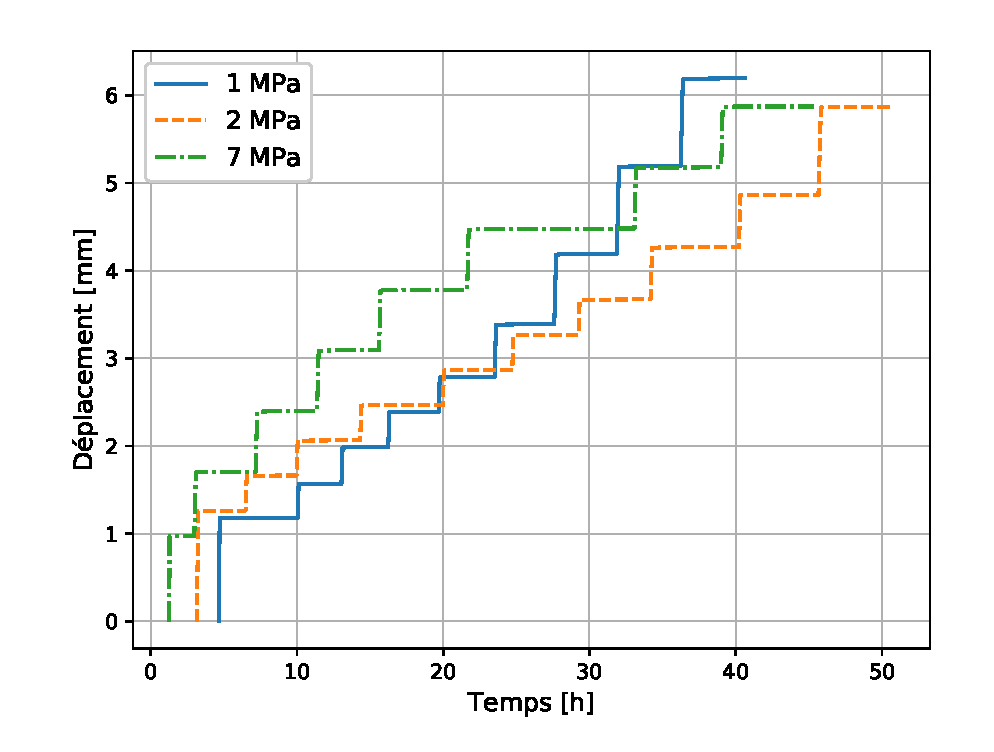
\includegraphics[width=0.49\textwidth]{displacement_time.eps}}\hfill
			\subfloat[]{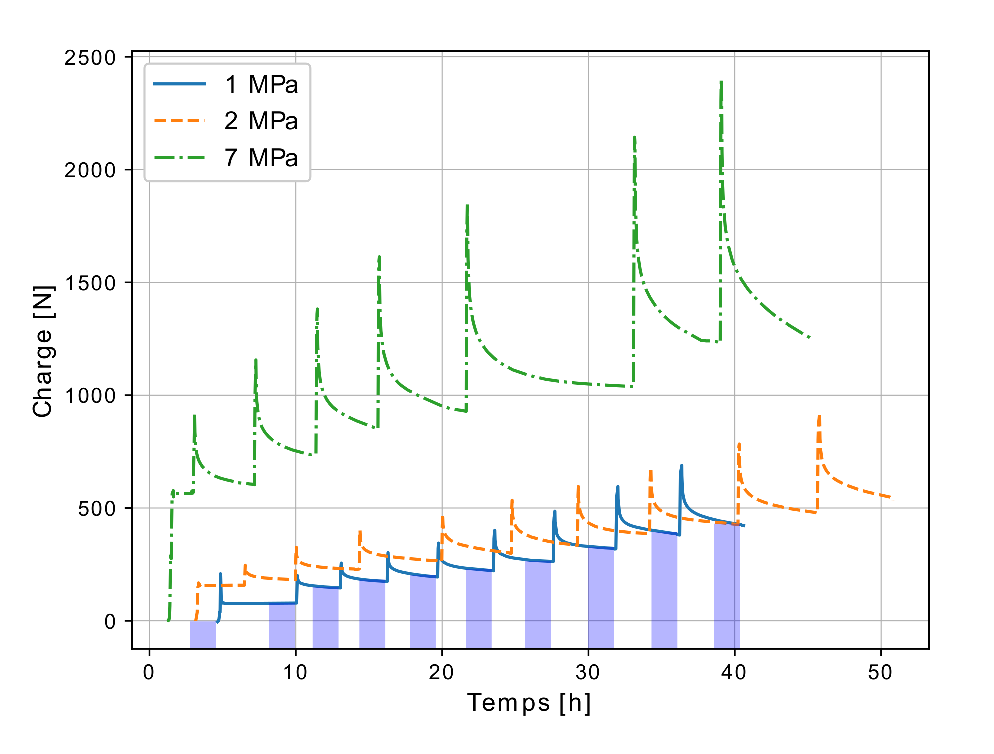
\includegraphics[width=0.49\textwidth]{load_time_scanTimes.eps}}
			\caption{\label{fig04:courbes_manip_temps}Courbes (a) du pilotage en déplacement du piston et (b) de la force mesurée sur le piston par rapport au temps pour l'ensemble des essais réalisés. Les zones en transparence bleue indiquent les temps de scan de tomographie pour l'essai dont la pression de confinement est \SI{1}{\mega\pascal}. Comme dans la suite, les essais sont triés par pression de confinement.}
		\end{figure}
		\\Il est observable sur la figure \ref{fig04:courbes_manip_temps} -(b) que l'échantillon dont le confinement est de \SI{1}{\mega\pascal} subit une pression de surconsolidation de \SI{2}{\mega\pascal}. Pour cela, la pression de confinement est augmentée jusqu'à cette valeur puis elle est ensuite diminuée jusqu'à la pression de confinement de \SI{1}{\mega\pascal} attendue pour l'essai.
	\subsection{Mesure des propriétés mécaniques des échantillons}
		Afin de comprendre la réponse globale de l'échantillon à la compression triaxiale, des calculs de contrainte et de déformation sont menés à partir des mesures de force et déplacement.
		\\Pour cela, des mesures de l'échantillon sont prises avant commencement du chargement par l'intermédiaire des images de tomographie. En effet, connaissant la taille des voxels, il est tout à fait possible de connaître la taille d'une structure en comptant le nombre de voxel selon la direction de la distance mesurée. L'échantillon est considéré à géométrie cylindrique parfaite (ce qui est relativement bien vérifié par l'observation des images de tomographie). Les mesures prises sont celle du diamètre de l'échantillon et de sa hauteur. En ce qui concerne le diamètre, plusieurs mesures sont faites sur la hauteur de l'échantillon et une valeur moyenne est choisie. Les mesures pour chacun des trois essais réalisés dans cette thèse sont présentées sur le tableau \ref{tab04:mesures_echantillons}.
		\begin{table}\centering
			\begin{tabular}{c@{\hspace{10mm}}c@{\hspace{10mm}}c}
				\hline
				Confinement & Diamètre [\si{\milli\meter}] & Hauteur [\si{\milli\meter}] \\\hline
				\SI{1}{\mega\pascal} & \num{10.10} & \num{21.30} \\
				\SI{2}{\mega\pascal} & \num{10.00} & \num{23.30} \\
				\SI{7}{\mega\pascal} & \num{10.15} & \num{22.70} \\\hline
			\end{tabular}
			\caption{\label{tab04:mesures_echantillons}Mesures des dimensions des échantillons.}
		\end{table}
		\\On fait l'hypothèse de l'homogénéité des essais. Alors, une méthode de calcul des contraintes ramenées à la surface initiale et déformations logarithmiques dans l'échantillon est de considérer la géométrie initiale de l'échantillon et la conservation de la géométrie cylindrique. Si cette dernière hypothèse s'avère vérifiée pour les petites déformations, elle n'est pas vérifiée lorsque la déformation atteint un niveau relativement élevé (cf. photographie du bas sur la figure \ref{fig04:deroulement_essai} -(g) et figure \ref{fig04:geometries_membrane}-(c)). Si $D_0$ est le diamètre initial de l'échantillon, $h_0$ sa hauteur initiale, $\Delta h$ le déplacement du piston par rapport à sa position initiale et $F$ la force mesurée par la capteur de force sur le piston, alors la contrainte axiale est définie selon l'équation (\ref{eq04:contrainte_echantillon}) et la déformation logarithmique axiale par l'équation (\ref{eq04:defo_echantillon}).
		\begin{equation}\label{eq04:contrainte_echantillon}
			\sigma_a = F \times \cfrac{4}{\pi D_0^2}
		\end{equation}
		\begin{equation}\label{eq04:defo_echantillon}
			\varepsilon_a = \ln\cfrac{h_0+\Delta h}{h_0}
		\end{equation}
		\`A partir de ces équations, il est possible d'utiliser les données présentées sur les graphes de la figure \ref{fig04:courbes_manip_temps} pour obtenir les courbes de contraintes-déformations présentées sur la figure \ref{fig04:courbes_manip_contrainte_defo}. Sur cette figure, la déformation axiale n'est pas mesurée lors de la mise sous pression de confinement puisque le piston reste immobile durant cette étape. Pour cette raison, les courbes ne sont valables qu'à partir du moment où le piston vient en contact de l'échantillon après la mise en confinement. Seule les parties valables des courbes sont tracées, ce qui explique l'absence d'information entre la déformation nulle et celle en début de courbe.
		\begin{figure}\centering
			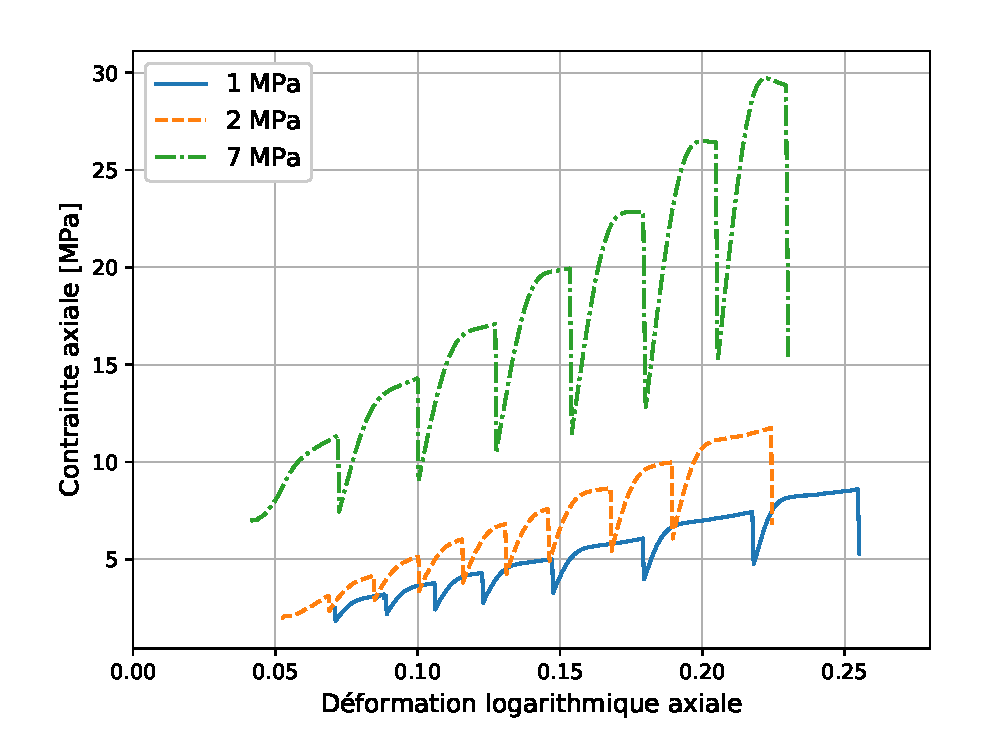
\includegraphics[width=0.7\linewidth]{stress_strain.eps}
			\caption{\label{fig04:courbes_manip_contrainte_defo}Courbes des contraintes-déformations de l'échantillon suivant la direction axiale du chargement.}
		\end{figure}
		\\L’évolution de la réponse mécanique au cours du temps permet de visualiser un comportement visco-élastique du milieu. Le comportement mécanique de l’échantillon conserve ce caractère visco-élastique jusqu’aux plus forts états de compression. Il est difficile dans cette réponse globale issue des capteurs de faire la part de la réponse mécanique de la cellule. La conception de la presse participant par exemple au frottement entre support et grains ou encore piston et support d’échantillon. Les courbes présentées sur les figures \ref{fig04:courbes_manip_temps}-(b) et \ref{fig04:courbes_manip_contrainte_defo} montrent cet effet visqueux par la relaxation de l'effort, et donc de la contrainte, lorsque la cinématique est figée. Lorsque le chargement axial reprend, après chaque arrêt du piston, la vitesse de déplacement du piston passe de manière quasi-instantanée d'une valeur nulle à une valeur de \SI{2}{\micro\meter\per\second} : cela engendre un ressaut de l'effort et de la contrainte à chaque reprise du chargement axial comme le montre les courbes.
		\\Il est observé également, par comparaison des courbes pour les trois valeurs de confinement, que la contrainte axiale est d'autant plus grande que la pression de confinement est grande pour des amplitudes de chargement fixées.
	\subsection{Essais hors tomographe}
		La compression de l'échantillon est menée en présence régulière d'un rayonnement X. Puisque la matière interagit aux rayons électromagnétiques de haute énergie, il est possible que la présence des rayons X modifie le comportement de l'échantillon si les rayons produits par le tomographe ont une énergie trop élevée. Afin de vérifier cette possibilité, des essais semblables à ceux menés au sein du tomographe ont été menés en dehors de la cabine d'exposition aux rayons X. La vitesse de sollicitation est toujours de \SI[per-mode=symbol]{2}{\micro\meter\per\second}. Les courbes contraintes-déformations de ces essais sont présentés sur la figure \ref{fig04:courbes_in_out}. Les courbes sur le graphe de gauche sont obtenues pour des pressions de confinement de \SI{250}{\kilo\pascal}, \SI{500}{\kilo\pascal}, \SI{1}{\mega\pascal}, \SI{2}{\mega\pascal}, \SI{4}{\mega\pascal} et \SI{7}{\mega\pascal}. Celles du graphe de droite sont les mêmes courbes (en traits pointillés) pour les pressions de confinement de \SI{1}{\mega\pascal}, \SI{2}{\mega\pascal} et \SI{7}{\mega\pascal} en présence des courbes (en traits continus) issues des essais menés dans le tomographe (essais \textit{in-situ}).
		\begin{figure}\centering
			\subfloat{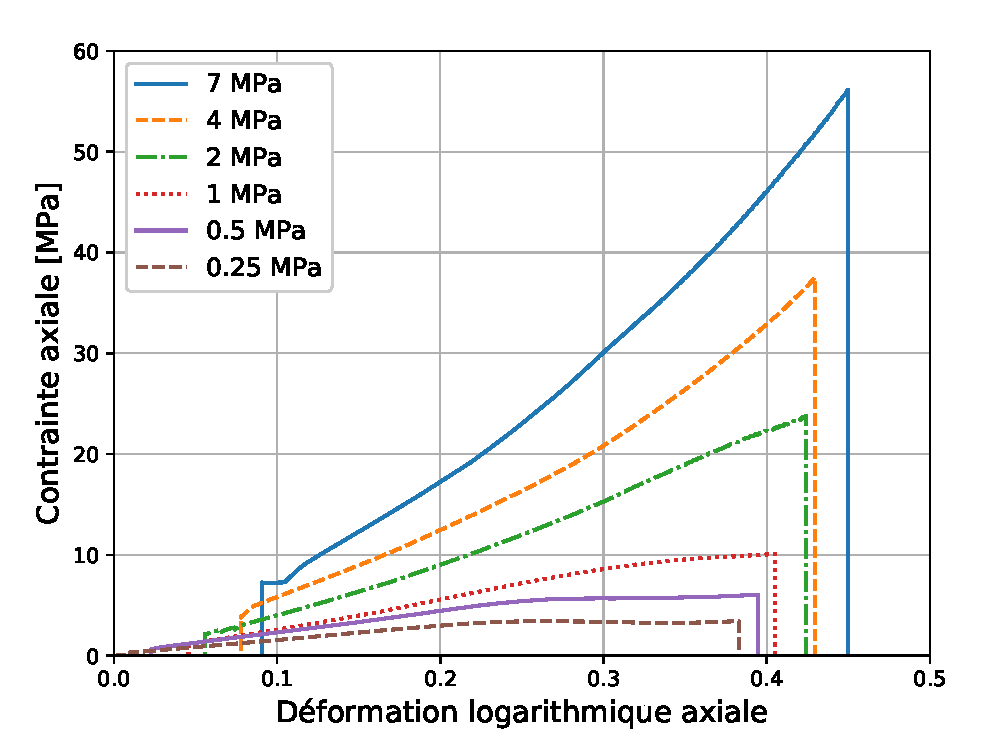
\includegraphics[width=.48\linewidth]{PS_stress-strain.eps}}\hfill
			\subfloat{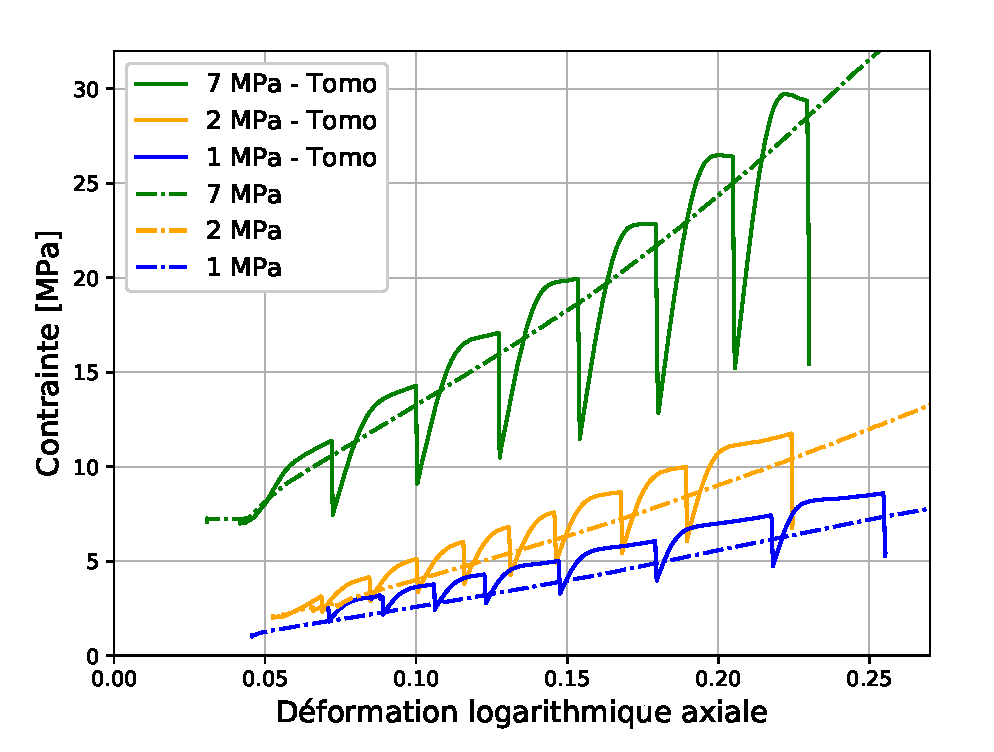
\includegraphics[width=.48\linewidth]{PS_in-out_stress-strain.eps}}
			\caption{\label{fig04:courbes_in_out}Courbes des contraintes-déformations pour (a) des essais de compression triaxiale à différentes pressions de confinement et sans interruption et (b) comparaison des essais menés dans le tomographe avec les mêmes essais menés en dehors.}
		\end{figure}
		Il est observé que dans les essais interrompus, la remise en charge (caractérisée par la fait que la vitesse de chargement imposée passe brusquement de \num{0} à \SI[per-mode=symbol]{2}{\micro\meter\per\second}), se traduit par un pic de contrainte jusqu'à une valeur supérieure à la contrainte obtenue pour le chargement monotone (sans interruption) pour la même déformation imposée. Cet effet est caractéristique du comportement viscoélastique et est observé notamment dans les essais de relaxation suite à un échelon en déformation. Il résulte du fait que le temps caractéristique de relaxation de l'échantillon (ou plutôt, de l'ensemble du dispositif incluant en particulier la cellule) est relativement faible par rapport à la vitesse de chargement. On voit également que le comportement à la remise en charge varie au cours du chargement, ce qui traduit la non-linéarité du système.
		\\L'analyse des graphes permet de constater, en particulier pour les pressions de confinement les plus faibles, que les courbes issues des essais ininterrompus semblent montrer une contrainte inférieure  à celles de la courbe maîtresse des essais interrompus. Plusieurs raisons peuvent être imaginées pour expliquer cette différence. Cet effet peut être rattaché à un phénomène mis en jeu lors de l'exposition du milieu granulaire aux rayons X. De plus, la précision de mesure des dimensions de l'échantillon est bien inférieure sur ces essais puisque la mesure au pied à coulisse permet une précision de l'ordre de \SI{0.02}{\milli\meter} alors que les images de tomographie permettent une précision inférieure à \SI{0.01}{\milli\meter}. Le rapport d'élancement de l'échantillon (rapport entre longueur et diamètre) avant essai est également un paramètre à prendre en compte. En ce qui concerne les essais hors tomographe, pour les pressions de confinement de \SI{1}{\mega\pascal}, \SI{2}{\mega\pascal} et \SI{7}{\mega\pascal}, les rapports d'élancement sont respectivement de \num{2.12}, \num{2.19} et \num{2.18}. Les essais, pour les mêmes pression de confinement, menés dans le tomographe sont réalisés sur des échantillons dont les rapports d'élancement sont de \num{2.11}, \num{2.33} et \num{2.24}. Une autre raison qui peut expliquer cette différence dans la mesure des contraintes est la condition de stockage des grains. En effet, les essais menés en dehors du tomographe ont été réalisés plusieurs mois après les essais menés dans le tomographe. Durant ces quelques mois, la poudre a été stockée à l'abri de la lumière, dans une salle dont la température est régulée mais dont l'humidité ne l'est pas. Il est donc possible que les propriétés des grains de polystyrène aient changées durant le temps de stockage par effet du vieillissement naturel. Enfin, les essais menés en dehors du tomographe sont réalisés sans interruptions, et donc ne subissent pas les mêmes contraintes de fluage et de relaxation.

\section{Tomographie à rayons X}\label{para04:tomo}
	\subsection{Matériel et protocole expérimental}
		Les scans sont réalisés par le microtomographe du laboratoire 3SR fabriqué par RX-Solutions (Annecy), avec une source Hamamatsu L12161-07 et un panneau de détection plat Varian.
		\\La figure \ref{fig04:manip_tomo} présente le dispositif d'acquisition avec le système de chargement tels qu'ils sont dans les expériences présentés dans ces travaux. On remarque que la distance entre la source et l'échantillon est minimale. Cette distance est réglable et permet de définir la résolution de l'image, déterminée en micromètre et correspondant à la taille d'un côté d'un voxel. Plus la distance est courte, meilleure est la résolution. Dans ces travaux, la résolution de \SI{9}{\micro\meter} est finalement la résolution maximale pour le dispositif du laboratoire.
		\begin{figure}\centering
			\includegraphics[]{tomo/manip.png}
			\caption{\label{fig04:manip_tomo}Photographie annotée du dispositif de tomographie du laboratoire 3SR utilisé dans ces travaux. Le fond a été mis en transparence pour des raisons de clarté.}
		\end{figure}
		Les paramètres d'acquisition des images de tomographie, pour les essais de compression triaxiale menés dans le tomographe, sont présentés dans le tableau \ref{tab04:param_tomo}. Le voltage et l'ampérage sont définis de manière à obtenir une puissance de faisceau des rayons X acceptables. Le faisceau doit être assez puissant pour traverser l'ensemble du dispositif expérimental et permettre un contraste entre les grains, l'air et la membrane. Il ne doit cependant pas être trop puissant pour ne pas saturer le détecteur.
		\\Le nombre de projection correspond au nombre de pas que le plateau tournant accomplit pour faire un tour complet. Pour chaque pas, le plateau reste fixe le temps de prendre au moins une radiographie de l'échantillon, que l'on nomme par la suite projection. Le nombre d'images par projection correspond au nombre de radiographies prises pour créer une projection. Plus le nombre de radiographies est grand, plus le bruit de l'image est diminué puisque le signal moyen de l'ensemble des radiographies prises est considéré pour établir la projection. De même, plus le nombre de projections augmente, plus la netteté de l'image reconstruite est élevée puisque le processus de reconstruction utilise plus de données brutes.
		\begin{table}\centering
			\begin{tabular}{rccc}
				\cline{2-4}
				& Confinement & Confinement & Confinement\\
				& \SI{1}{\mega\pascal} & \SI{2}{\mega\pascal} & \SI{7}{\mega\pascal}\\\hline
				Taille du voxel [\si{\micro\meter}] & 9.00 & 9.00 & 9.00 \\\hline
				Voltage [\si{\kilo\volt}] & 80 & 80 & 80 \\\hline
				Ampérage [\si{\micro\ampere}] & 112 & 113 & 125 \\\hline
				Nombre de projections & 1440 & 1440 & 1120 \\\hline
				Images par projection & 3 & 3 & 6 \\\hline
				\multirow{2}{*}{Volume [\si{\voxel^3}]} & $1445\times 1445$ & $1445\times 1445$ & $1444\times 1444$ \\
				& $\times 1600$ & $\times 1600$ & $\times 1650$ \\\hline
			\end{tabular}
			\caption{\label{tab04:param_tomo}Paramètres d'acquisition des images de tomographie pour les différents essais réalisés \textit{in situ}.}
		\end{table}
	\subsection{Utilisation des projections et reconstruction}
		La reconstruction des images de tomographie à partir des projections est expliquée au paragraphe \ref{para03:tomo}. Seulement, l'étape de reconstruction ne consiste pas uniquement à la superposition des différentes projections. Il est nécessaire de corriger certains artefacts liés à l'acquisition des images dans le même temps. Cela a été réalisé par l'intermédiaire du programme XAct.
		\\Un scan est caractérisé par l'acquisition de l'ensemble des projections, et donc à la prise de radiographies sous une multitude d'angles d'acquisition de $0$ à $360$ degrés. Comme pour toute prise d'images, il est primordial que le sujet ne bouge pas en cours d'acquisition afin d'assurer une netteté correcte de l'image. Compte tenu des performances du tomographe du laboratoire utilisé, du nombre de projections par scan et du nombre d'images par projection, le temps de scan est plutôt conséquent : il faut compter en moyenne deux heures. Durant ces deux heures, il est possible que la microstructure de l'échantillon ait été modifiée ou que l'échantillon se soit déplacé. La microstructure étant stable lors des phases de scan, seul le déplacement de l'échantillon en cours d'acquisition des projections est observé. Afin de tenir compte de ce déplacement en cours d'acquisition, trente-deux projections sont réalisées sur des angles linéairement répartis entre $0$ et $360$ degrés et sur des positions déjà traitées. Un calcul de corrélation entre les projections "normales" et les projections en fin de scan permet d'établir le déplacement de l'échantillon en cours d'acquisition et de corriger la position de la microstructure lors de la reconstruction.
		\begin{figure}\centering
			\subfloat[Exemple de projection radiographique]{\includegraphics[width=.6\textwidth]{tomo/proj_rescale_15.jpg}}\\
			\subfloat[Coupe horizontale après reconstruction]{\includegraphics[width=.55\textwidth]{tomo/slice.jpg}}\hfill
			\subfloat[Volume 3D après reconstruction]{\includegraphics[width=.35\textwidth]{tomo/3D_0_00.jpg}}
			\caption{\label{fig04:reconstruction_tomo}Les projections (a) issues de la tomographie permettent d'obtenir, par reconstruction, des coupes internes de l'échantillon (b) et la microstructure du volume complet (c).}
		\end{figure}
		\begin{figure}\centering
			\subfloat[\SI{1}{\mega\pascal} - $E_0$]{\includegraphics[width=0.33\textwidth]{3d_samples/1_00_resized.jpg}}\hfill
			\subfloat[\SI{1}{\mega\pascal} - $E_C$]{\includegraphics[width=0.33\textwidth]{3d_samples/1_0Pc_resized.jpg}}\hfill
			\subfloat[\SI{1}{\mega\pascal} - $E_F$]{\includegraphics[width=0.33\textwidth]{3d_samples/1_8_resized.jpg}}
			\\
			\subfloat[\SI{2}{\mega\pascal} - $E_0$]{\includegraphics[width=0.33\textwidth]{3d_samples/2_00_resized.jpg}}\hfill
			\subfloat[\SI{2}{\mega\pascal} - $E_C$]{\includegraphics[width=0.33\textwidth]{3d_samples/2_0Pc_resized.jpg}}\hfill
			\subfloat[\SI{2}{\mega\pascal} - $E_F$]{\includegraphics[width=0.33\textwidth]{3d_samples/2_9_resized.jpg}}
			\\
			\subfloat[\SI{7}{\mega\pascal} - $E_0$]{\includegraphics[width=0.33\textwidth]{3d_samples/7_00_resized.jpg}}\hfill
			\subfloat[\SI{7}{\mega\pascal} - $E_C$]{\includegraphics[width=0.33\textwidth]{3d_samples/7_0Pc_resized.jpg}}\hfill
			\subfloat[\SI{7}{\mega\pascal} - $E_F$]{\includegraphics[width=0.33\textwidth]{3d_samples/7_7_resized.jpg}}
			\caption{\label{fig04:samples_3D}Représentation des reconstructions volumiques de chacun des échantillons (\SI{1}{\mega\pascal}, \SI{2}{\mega\pascal} et \SI{7}{\mega\pascal} en fonction de la pression de confinement) dans différents états de compression : $E_0$ est l'état non comprimé (dit naturel), $E_C$ est l'état de compression isotrope (après la mise en confinement) et $E_F$ est l'état final (après le dernier chargement axial).}
		\end{figure}
		\\\`A la suite de la correction liée au déplacement de l'échantillon, la superposition des projections peut être faite. Avant cela, un échantillonnage du signal est réalisé pour former des reconstructions au format 16-bit. Pour cela, des valeurs limites lues par le détecteur des rayons X sont choisies. Toutes les valeurs inférieures à la plus petite valeur limite sont considérées égales à 0, celles supérieures à la plus grande valeur limite sont considérées égales à \num{65535} ($2^{16}-1$). Les valeurs intermédiaires suivent la même répartition linéaire que celle du signal d'origine entre les deux valeurs limites.
		La figure \ref{fig04:reconstruction_tomo} (a) présente un exemple de projection obtenu lors d'un scan dans le tomographe. L'ensemble des corrections appliquées aux projections et la superposition des projections permettent d'obtenir la microstructure du volume scanné. Les figures \ref{fig04:reconstruction_tomo} (b) et (c) en sont des exemples. La première représente une coupe dans le volume suivant à une hauteur donnée de l'échantillon tandis que la seconde représente le volume. La figure \ref{fig04:samples_3D} présente quant à elle les volumes des échantillons avant la mise en confinement, après la mise en confinement et après le chargement axial final pour chacun des trois essais.

\section{Caractérisation des échantillons}
	Les images de tomographie acquises durant les essais de compression triaxiale vont permettre d'analyser la microstructure des échantillons puisqu'elles caractérisent directement l'état de densité de ces derniers. Cependant l'utilisation immédiate de ces images n'est pas recommandée et un traitement du signal de chacune d'elles est nécessaire pour optimiser les méthodes d'analyse. Ces méthodes consistent à cartographier les états de densité et de déformation (en menant des calculs de corrélation de volumes numériques) au sein de l'échantillon afin de permettre une étude locale, mais également globale, des échantillons en cours de compression.
	\subsection{Post-traitement des images de tomographie}
		\subsubsection{Traitement et optimisation des images}
			Les images directement issues des reconstructions de tomographie ne sont pas adaptées pour être analysées. En effet, en fonction du protocole suivi pour la tomographie et des limites du tomographe, les images peuvent se retrouver mal contrastées et bruitées. Il est alors nécessaire de corriger la qualité de ces images par des méthodes simples et bien connues. Les reconstructions de tomographie sont des images au format 8-bit. L'ensemble des tâches présentées ici sont adaptées à ce format d'image. La plage d'intensité des voxels pour ce format est l'ensemble des entiers positifs allant de $0$ à $255$ compris.
			\\La tomographie ayant été réalisée sur un échantillon comprimé d'une poudre constituée d'un seul matériau, nous nous attendons à observer un signal bimodal. En effet, le milieu observé est constitué de deux éléments : le polystyrène qui absorbe assez bien les rayons X et l'air comblant les porosités qui absorbe très peu ces mêmes rayons. Puisque la tomographie est basée sur une technique d'absorption des rayons X (cf. paragraphe \ref{para03:tomo}), il est logique d'observer une grande partie des voxels ayant une intensité relativement grande et une une autre grande partie relativement faible.
			\\Dans le cas idéal, avec des instruments de très grande résolution, des capteurs très performants et un milieu observé assurément isolé des conditions extérieures et complètement biphasique, l'histogramme des images reconstruites par tomographie devrait présenter deux pics uniques et totalisant l'ensemble des voxels (cf. paragraphe \ref{para03:traitement_image}). Parce que ces conditions ne sont pas réunies, on observe un signal plus lissé et plus bruité. L'histogramme présente alors deux pics plus ou moins étalés sur l'ensemble des valeurs d'intensité des voxels. Afin d'analyser et d'utiliser les images de la manière la plus pertinente possible, il est nécessaire de se rapprocher du cadre idéal pour un milieu biphasique. Il est alors nécessaire de minimiser la largeur des pics de l'histogramme et de les éloigner le plus possible l'un de l'autre en augmentant le contraste. La figure \ref{fig04:contrast_enhancement_filtering} illustre l'ensemble des tâches accomplies afin de permettre cela. Chacune de ces étapes est décrite dans les paragraphes qui suivent.
			\begin{figure}\centering
				\subfloat[Image d'origine]{\includegraphics[width=.27\textwidth]{contrast_enhancement_filtering/00-orig_0142_resized.png}}
				\subfloat[Histogramme de l'image d'origine]{\includegraphics[width=.67\textwidth]{contrast_enhancement_filtering/00-orig_hist.eps}}\\
				\subfloat[Accentuation du contraste]{\includegraphics[width=.27\textwidth]{contrast_enhancement_filtering/01-contrast_0142_resized.png}}
				\subfloat[Histogramme de l'image avec accentuation du contraste]{\includegraphics[width=.67\textwidth]{contrast_enhancement_filtering/01-contrast_hist.eps}}\\
				\subfloat[Filtre bilatéral]{\includegraphics[width=.27\textwidth]{contrast_enhancement_filtering/02-bilat_0142_resized.png}}
				\subfloat[Histogramme de l'image avec filtre bilatéral]{\includegraphics[width=.67\textwidth]{contrast_enhancement_filtering/02-bilat_hist.eps}}\\
				\subfloat[Filtre de variation totale]{\includegraphics[width=.27\textwidth]{contrast_enhancement_filtering/03-bilatTV_0142_resized.png}}
				\subfloat[Histogramme de l'image avec filtre de variation totale]{\includegraphics[width=.67\textwidth]{contrast_enhancement_filtering/03-bilatTV_hist.eps}}
				\caption{\label{fig04:contrast_enhancement_filtering}Illustration du traitement des images issues des reconstructions de tomographie. A gauche, une coupe de l'image 3D. A droite, l'histogramme associé à cette image 3D.}
			\end{figure}
			\paragraph{}La première étape consiste à atténuer le bruit aux extrémités de la plage de données du signal et procéder à un renforcement du contraste. Cette étape est illustrée sur les figures \ref{fig04:contrast_enhancement_filtering}-(c) et (d). Il est considéré que le bruit est présent sur l'ensemble de la plage de données du signal (pour toutes les nuances de gris) alors que l'information structurale de l'échantillon n'est présente que sur une zone plus restreinte et centrée sur cette même plage de données. Pour les travaux de cette thèse, il a été considéré que l'information structurale est donnée dans les \num{99} percentiles centrés sur la plage de données (qui va de \num{0} à \num{255}). Considérant cela, les voxels ayant une intensité plus faible que l'intensité du voxel à \num{0.5} percentile ($I_\textrm{min}$) prennent la valeur de ce dernier. Les voxels ayant une intensité plus grande que le voxel à \num{99.5} percentile ($I_\textrm{max}$) prennent la valeur de ce dernier. Comme la nouvelle plage d'intensités prises par les voxels est désormais plus petite que celle d'origine ($I_\textrm{max}-I_\textrm{min} < 255$), il est nécessaire d'étaler de manière uniforme le nouveau signal entre les valeurs $0$ et $255$. L'équation (\ref{eq04:contraste}) permet de déterminer la valeur de l'intensité d'un voxel après renforcement du contraste ($I_\textrm{après}$) en fonction de l'intensité du même voxel dans l'image d'origine ($I_\textrm{avant}$).
			\begin{equation}\label{eq04:contraste}
			I_\textrm{après} = \cfrac{I_\textrm{avant} - I_\textrm{min}}{I_\textrm{max} - I_\textrm{min}}\times 255
			\end{equation}
			\paragraph{}La seconde étape, illustrée sur les figures \ref{fig04:contrast_enhancement_filtering}-(e), (f), (g) et (h), consiste à lisser le signal de manière à éliminer le bruit au sein de chaque phase. Cela se fait par l'intermédiaire de filtres qui engendrent un flou dans l'image. Cette étape permet de mieux identifier les pics présents dans l'histogramme mais peut avoir pour conséquence de rendre la limite entre ces deux pics plus difficile à établir. Les voxels qui sont proches des frontières entre les deux phases vont également subir le flou et vont prendre des valeurs intermédiaires. Sur l'histogramme, les deux pics seront donc mieux définis car plus fins mais le minimum situé entre ces deux pics sera augmenté à cause des voxels aux frontières. Un moyen d'éviter ce dernier effet est d'engendrer un flou qui tient compte des bordures et donc des zones à fort contraste. Pour cette raison, les filtres de lissage "bilatéral" \citep{tomasi_bilateral_1998} et "variation totale" \citep{chambolle_algorithm_2004} ont été choisis. Le filtre bilatéral modifie la valeur des voxels en moyennant la valeur des voxels voisins qui n'ont pas tous le même poids dans la moyenne. Le poids attribué à chaque voxel voisin dépend de la distance euclidienne avec le voxel en cours de traitement (plus il est proche et plus il compte dans la moyenne - il s'agit de la même approche que pour un lissage gaussien) mais également de la différence de niveau de gris entre les deux voxels (plus la différence est grande, moins il compte dans la moyenne - c'est cette propriété qui permet de conserver les frontières entre les différentes phases). Le filtre de variation totale est quant à lui basé sur la recherche d'une image qui minimise la variation totale du signal tout en restant le plus proche possible de l'image de départ ; il s'agit là encore d'un processus qui conserve plutôt bien les frontières entre différentes phases. Le choix a été fait d'utiliser successivement ces deux filtres afin de minimiser le temps et le coût de calcul. En effet, le filtre bilatéral semble être le plus efficace et suffit à lui seul à corriger les images. Cependant, l'ensemble des calculs non-linéaires qu'il doit fournir rend la tâche non adaptée au projet. Il est possible de l'utiliser sans engendrer trop d'énergie de calcul avec des paramètres permettant une correction relativement moyenne. Le filtre de variation totale permet de finaliser le lissage plus rapidement grâce aux calculs qui sont, cette fois-ci, linéaires.
			\paragraph{}La figure \ref{fig04:contrast_enhancement_filtering} montre l'effet de chacune des corrections sur une coupe de l'image 3D et son histogramme. Il est à noter que cette figure illustre les effets des corrections sur une image plane bien que ces corrections soient dans les trois directions de l'espace. Il est en effet difficile de visualiser des images 3D sur un support plan. Pour cette raison, des coupes seront exposées dans les plans les plus faciles à extraire : ce seront ici des coupes dans le plan ($Oxy$) d'un repère cartésien pour les reconstructions de tomographie. En effet, les images reconstruites ont été enregistrées sous la forme de "stack" qui correspond à un empilement d'image dans la direction de l'axe ($Oz$). Le filtre bilatéral est celui de la bibliothèque Python "scikit-image" \citep{scikit_image} et a pour paramètres : un écart-type spatial de \SI{2}{\voxel}, un écart-type d'intensité de \num{0.007} et une fenêtre de travail de \SI{6}{\voxel} de côtés. Le filtre de variation totale, issu de la même bibliothèque Python, a pour paramètre un poids de $0.1$. Ces valeurs ont été choisies de manière purement qualitative. Une comparaison des histogrammes de l'image d'origine (figure \ref{fig04:contrast_enhancement_filtering}-(b)) et de l'image traitée (figure \ref{fig04:contrast_enhancement_filtering}-(h)) permet d'identifier une augmentation de la grandeur des pics et une diminution de leur largeur. Ces éléments prouvent que le processus employé transforme l'image d'origine en une image plus facile à binariser, facilitant ainsi la reconnaissance des deux phases en présence.
		\subsubsection{Binarisation par seuillage automatique}
			\label{para04:seuillage}
			\paragraph{}La figure \ref{fig04:contrast_enhancement_filtering}-(h) met en évidence qu'une relativement grande partie des voxels ont des intensités comprises entre les deux valeurs caractérisant les pics, formant ainsi un plateau entre ceux-ci. La distinction entre les deux phases nécessite de déterminer une valeur limite sur ce plateau. La détermination de cette valeur limite, appelée valeur seuil, peut être réalisée en utilisant une méthode de seuillage automatique (cf. paragraphe \ref{para03:threshold}). Deux méthodes couramment utilisées sont décrites ici.
			\paragraph{}La première méthode de seuillage automatique est celle de \citet{otsu_threshold_1979}. Otsu montre que dans le cadre d'un signal bimodal, donc avec deux classes, une valeur seuil optimale est celle qui minimise la variance intra-classe\footnote{La variance intra-classe correspond à la moyenne des variances de chacune des classes.} du signal. Cela revient à maximiser la variance inter-classe\footnote{La variance inter-classe correspond à la variance des moyennes de chacune des classes.}. D'un point de vue pratique, la méthode de seuillage d'Otsu consiste à seuiller l'image pour toutes les valeurs possible de seuillage (de \num{0} à \num{255} pour une image au format 8-bit), de calculer les valeurs moyennes de chacune des phases et de mesurer la variance des moyennes obtenues. Une fois que cela est fait pour chacune des valeurs seuil possible, c'est la valeur seuil pour laquelle la variance est la plus grande qui va être choisie comme valeur seuil qui permet d'identifier les différentes phases.
			\paragraph{}La seconde méthode de seuillage a été développée par \citet{kittler_minimum_1986} et est souvent dénommée "méthode de seuillage par minimisation de l'erreur". Avec cette méthode, chacun des deux modes est approximé par une gaussienne. La valeur de seuil optimale est choisie lorsque le chevauchement entre les gaussiennes est minimal.
			\paragraph{}Les deux méthodes décrites ici ont chacune leurs avantages et sont toutes deux adaptées à la segmentation des images présentant deux phases (signal bimodal). Malgré cela, les méthodes de calcul de la valeur seuil étant différentes, les deux méthodes de seuillages n'indiquent pas les mêmes seuils. \'Evidemment, ces valeurs restent proches l'une de l'autre mais la différence est suffisante pour engendrer des erreurs d'analyse des images binaires par la suite. Il est difficile de définir la méthode la mieux adaptée puisque cela dépend directement du signal des images et de leur qualité. Dans certains cas la méthode d'Otsu sera plus adaptée que celle de Kittler et Illingworth, dans d'autres cas ce sera l'inverse. Il a été remarqué cependant que pour un milieu confiné donné (même milieu granulaire, même densité), avec des images issues d'un même protocole expérimental (même tomographe, même méthode de reconstruction, etc.), la qualité du seuillage reste la même pour différentes images. Il semble donc que la méthode à choisir dépende du milieu granulaire observé, de sa densité apparente et du protocole suivi pour la réalisation de la tomographie. Il est, par conséquent, nécessaire de définir une méthode de seuillage pour chaque échantillon observé par tomographie et pour chaque état de compression.
			\paragraph{}Il reste à résoudre un problème. Comment choisir parmi les deux méthodes de seuillage automatique ? Comment faire lorsque les deux méthodes ne donnent pas un résultats approprié ? On considère d'abord que les voxels les plus clairs (valeurs proches de \num{255}) sont ceux qui caractérisent le matériau constituant le milieu granulaire et ceux qui sont sombres (valeurs proches de \num{0}) caractérisent les porosités. Les images de tomographie utilisées dans ces travaux présentent toujours le même constat : le seuillage par la méthode d'Otsu présente une valeur seuil légèrement différente de celle de Kittler, de sorte que lorsque l'une semble trop basse l'autre semble trop élevée. Ainsi, en seuillant l'image par une méthode quelques voxels de porosité sont considérés comme de la matière tandis qu'avec la seconde méthode c'est l'inverse.
			\paragraph{}Une manière de régler le problème de choix entre les deux méthodes de seuillage est d'utiliser une moyenne pondérée. En faisant cela, un seul paramètre suffit pour déterminer la valeur seuil. Cette moyenne est calculée suivant l'équation (\ref{eq04:seuillage}) :
			\begin{equation}\label{eq04:seuillage}
			S = \alpha\cdot S_\textrm{Otsu} + \left(1-\alpha\right)\cdot S_\textrm{Kittler}
			\end{equation}
			avec, $S$ la valeur de seuil choisie entre la valeur seuil d'Otsu $S_\textrm{Otsu}$ et celle de Kittler $S_\textrm{Kittler}$, et $\alpha$ le paramètre de pondération qui représente le poids de la méthode d'Otsu sur cette moyenne. Comme il l'a été dit, la valeur de seuil ne semble pas varier pour un même milieu confiné. Il suffit donc de déterminer la valeur du coefficient $\alpha$ pour chaque essai de compression accompli au sein du tomographe, et pour chaque état de compression. C'est ce qui a été fait. Des tests ont été menés sur des images issues des différentes campagnes d'essais afin de déterminer les valeurs de $\alpha$. L'évaluation de la valeur de seuillage optimale a été entièrement qualitative, par méthode de visualisation et comparaison des images originales et binaires. Un réajustement de la valeur de $\alpha$ est nécessaire lors de toute analyse d'images nouvelles (issues d'un nouvel essai).
			\begin{table}\centering
				\begin{tabular}{ccc}
					\hline
					& \multicolumn{2}{c}{Milieu granulaire avec}\\
					& grains de polystyrène & grains d'amidon \\\hline
					Valeur du coefficient $\alpha$ & $0.2$ & $0.4$ \\\hline
				\end{tabular}
				\caption{\label{tab04:valeur_alpha}Valeurs du coefficient de pondération de la méthode d'Otsu concernant la moyenne pondérée avec la méthode de Kittler.}
			\end{table}
			Le tableau \ref{tab04:valeur_alpha} mentionne les valeurs moyennes utilisées pour calculer la valeur de seuillage la plus appropriée au milieu observé. On remarque que la méthode de Kittler semble, sur les échantillons étudiés dans cette thèse, plus pertinente que la méthode d'Otsu ($\alpha < 0.5$) et que la morphologie des grains et la granulométrie semblent jouer un rôle dans le choix de ce coefficient et donc de la valeur seuil.
			\begin{figure}\centering
				\subfloat[$\alpha = 1.0\quad\left( S=120 \right)$]{
					\includegraphics[width=0.3\textwidth]{threshold/contour_120_0142.png}}\hfill
				\subfloat[$\alpha = 0.4\quad\left( S=126 \right)$]{
					\includegraphics[width=0.3\textwidth]{threshold/contour_126_0142.png}}\hfill
				\subfloat[$\alpha = 0.0\quad\left( S=130 \right)$]{
					\includegraphics[width=0.3\textwidth]{threshold/contour_130_0142.png}}
				\\
				\subfloat[Visualisation sur l'histogramme de l'image 3D associée]{
					\includegraphics[width=0.8\textwidth]{threshold/histogram.eps}
				}
				\caption{\label{fig04:seuillage_polystyrene}Résultat du seuillage automatique avec différentes valeurs de $\alpha$. $S$ désigne la valeur de seuillage obtenue. Les figures (a), (b) et (c) représente une coupe de l'image 3D sur laquelle est superposée le contour des zones seuillées (en rouge).}
%				$\begin{array}{c}\alpha = 0.4\\S_{\alpha{_1}} = 120\end{array}$
			\end{figure}
			\\Les figures \ref{fig04:seuillage_polystyrene}-(a) à (c) illustrent l'effet du paramètre $\alpha$ sur une coupe d'image de tomographie d'un milieu constitué de grains de polystyrène. La méthode d'Otsu (figure \ref{fig04:seuillage_polystyrene}-(a)) a tendance à diminuer la porosité. C'est l'inverse avec la méthode de Kittler (figure \ref{fig04:seuillage_polystyrene}-(c)). La moyenne pondérée des deux méthodes avec $\alpha=0.4$ permet de considérer le seuillage optimal. La figure \ref{fig04:seuillage_polystyrene}-(d) permet d'observer l'effet du seuillage directement sur l'histogramme.
	\subsection{Analyse de densité}
		L'image seuillée obtenue par binarisation est une image représentant les deux phases de l'échantillon : les voxels blancs représentent les grains tandis que les voxels noirs représentent les porosité à l'intérieur du milieu granulaire. \`A partir de cette information sur l'image binaire, il est possible de mesurer la densité\footnote{Il s'agit en fait de calculer la fraction volumique solide qui peut être considérée comme identique à la densité dans le cas d'un milieu constitué d'un seul matériau incompressible.} $d$ du milieu dans un volume donné $V$, constitué de $V_G$ voxels blancs et $V_P$ voxels noirs, grâce à l'équation (\ref{eq04:calcul_densite}) :
		\begin{equation}\label{eq04:calcul_densite}
			d = \cfrac{V_G}{V} = \cfrac{V_G}{V_G+V_P}
		\end{equation}
		Lorsque l'équation (\ref{eq04:calcul_densite}) est utilisée sur le volume entier de l'échantillon, la densité obtenue correspond alors à la densité apparente de l'échantillon $d_\textrm{ech}$ qui est calculée expérimentalement avec la masse de grain introduite $m$, la masse volumique du matériau constituant les grains $\rho$ et le volume de l'échantillon $V_\textrm{ech}$ par la relation (\ref{eq04:mesure_densite}) :
		\begin{equation}\label{eq04:mesure_densite}
			d_\textrm{ech} = \cfrac{m}{\rho V_\textrm{ech}}
		\end{equation}
		Cette dernière équation donne une information sur la densité de l'échantillon dans sa globalité. La figure \ref{fig04:bulkDensities} montre l'évolution de la densité relative globale des échantillons pour chacun des essais et calculée à partir de (\ref{eq04:calcul_densite}) sur l'ensemble des volumes issus des scans de tomographie. Le graphe représente l'évolution de cette densité en fonction de la déformations axiale imposée. Alors que la densité de l'échantillon subissant une pression de confinement de \SI{7}{\mega\pascal} est une contribution presque linéaire de la déformation axiale, il n'en est pas de même pour les pressions de confinement inférieures (\num{1} et \SI{2}{\mega\pascal}). Une explication possible à cela \citep{pavier_caracterisation_1998} est que l'élévation de la pression de confinement favorise la déformation des grains (qui sont ductiles) dans les zones de fortes contraintes de cisaillement en dépit du glissement pur (sans déformation). Ainsi, les échantillons des essais menés avec les plus faibles pressions de confinement seraient plus sensibles aux effets de dilatance et pourraient même présenter des bandes de cisaillement (cf. paragraphe \ref{para03:dilatance}). Ces raisons peuvent même expliquer la formation d'une géométrie "en tonneau" de l'échantillon pour les grandes déformations axiales (augmentation du volume apparent dans les zones de fort cisaillement). Il faut cependant rester vigilant sur ces résultats puisque, pour rappel, le calcul de densité est basée sur l'étude d'images binaires. Si la méthode de seuillage n'est pas adaptée pour l'un des états de chargement alors le calcul de densité s'en retrouve faussé. Or, bien que visuellement le seuillage des volumes les plus comprimés semble correct, la méthode de seuillage automatique utilisée dans ces travaux (cf. partie précédente) ne sera pas aussi efficace d'un état de compression à un autre.
		\begin{figure}\centering
			\includegraphics[width=0.8\textwidth]{bulkDensities/bulk_densities.eps}
			\caption{\label{fig04:bulkDensities}\'Evolution de la densité apparente des différents échantillons par rapport à la déformation axiale.}
		\end{figure}
		\paragraph{}
		Il peut être également intéressant d'étudier la densité de manière plus locale en utilisant l'équation (\ref{eq04:calcul_densite}) sur des volumes suffisamment petits pour suivre localement la densification de l'échantillon au cours de la compression. La discrétisation du volume total de l'échantillon $V_\textrm{ech}$ en sous-volumes $V_{\textrm{loc},i}$ selon les conditions données par (\ref{eq04:conditions_Vlocaux}) permet de générer un champ de densité dans l'échantillon.
		\begin{equation}\label{eq04:conditions_Vlocaux}
			\bigcup_i V_{\textrm{loc},i} = V_\textrm{ech}
			\qquad\text{et}\qquad
			\bigcap_i V_{\textrm{loc},i} = \emptyset
		\end{equation}
		Les images de tomographie obtenues dans ces travaux ont une dimension moyenne de $1450 \times 1450 \times 1600$ voxels et sont au format 8-bit : leur taille moyenne en mémoire est donc de $1450 \times 1450 \times 1600 / 2^{20} = 3208$ Mo ($2^{20}$ représente la valeur de $1$ Mo) soit encore \num{3.2} Go. Une discrétisation en sous-volumes cubiques de côté \SI{10}{\voxel} permet de travailler avec une image de dimension $145 \times 145 \times 160$ voxels et dont la taille en mémoire ne vaut plus que \num{3.2} Mo. En plus de cela, sachant que la taille des voxels dans les travaux menés dans cette thèse est de \SI{9}{\micro\meter}, les sous-volumes cubiques d'arête \SI{10}{\voxel} dans l'image numérique représentent finalement des sous-volumes dont les côtés ont une longueur de \SI{90}{\micro\meter} dans l'échantillon réel. Cette longueur est moins grande que celle de la taille moyenne des grains de polystyrène. Finalement, pour la définition donnée précédemment de sous-volumes, la "compression" du champ de densité donné directement par la tomographie permet d'obtenir un nouveau champ de densité dont la résolution permet encore d'informer localement de l'état de densification de l'échantillon à l'échelle du grain. Des cartes 3D des densités, comme celles présentées à titre d'exemple sur la figure \ref{fig04:densities_3D}, peuvent alors être calculées et permettre une analyse rapide et efficace de la densification des différents échantillons en cours de compression.
		\begin{figure}\centering
			\subfloat[\SI{1}{\mega\pascal} - $E_0$]{\includegraphics[width=0.27\textwidth]{3d_densities/1_00_resized.jpg}}\hfill
			\subfloat[\SI{1}{\mega\pascal} - $E_C$]{\includegraphics[width=0.27\textwidth]{3d_densities/1_0Pc_resized.jpg}}\hfill
			\subfloat[\SI{1}{\mega\pascal} - $E_F$]{\includegraphics[width=0.27\textwidth]{3d_densities/1_8_resized.jpg}}
			\\
			\subfloat[\SI{2}{\mega\pascal} - $E_0$]{\includegraphics[width=0.27\textwidth]{3d_densities/2_00_resized.jpg}}\hfill
			\subfloat[\SI{2}{\mega\pascal} - $E_C$]{\includegraphics[width=0.27\textwidth]{3d_densities/2_0Pc_resized.jpg}}\hfill
			\subfloat[\SI{2}{\mega\pascal} - $E_F$]{\includegraphics[width=0.27\textwidth]{3d_densities/2_9_resized.jpg}}
			\\
			\subfloat[\SI{7}{\mega\pascal} - $E_0$]{\includegraphics[width=0.27\textwidth]{3d_densities/7_00_resized.jpg}}\hfill
			\subfloat[\SI{7}{\mega\pascal} - $E_C$]{\includegraphics[width=0.27\textwidth]{3d_densities/7_0Pc_resized.jpg}}\hfill
			\subfloat[\SI{7}{\mega\pascal} - $E_F$]{\includegraphics[width=0.27\textwidth]{3d_densities/7_7_resized.jpg}}
			\caption{\label{fig04:densities_3D}Représentation des champs de densité de chacun des échantillons dans différents états de compression en utilisant le même formalisme que pour la figure \ref{fig04:samples_3D}. La résolution de la mesure du champ est telle qu'un volume élémentaire de densité est un cube d'arrête de \SI{90}{\micro\meter}. L'échelle de couleur va du bleu pour une densité nulle jusqu'à du rouge pour une densité relative de $1$.}
		\end{figure}
	
	\subsection{Calcul de la cinématique}\label{para04:cinematique}
		En plus de l'évolution de la densité, il est possible de déterminer l'évolution des déformations dans l'échantillon en cours de compression. Cela est rendu possible par l'intermédiaire de la corrélation d'image 3D. Comme expliqué dans le paragraphe \ref{para03:DIC}, la corrélation des volumes issus de la tomographie permet d'obtenir un champ vectoriel des déplacements au sein des volumes. La cohérence des champs de déplacement obtenus a été vérifiée visuellement sur plusieurs sous-volumes choisis aléatoirement dans l'échantillon scanné. Les déplacements obtenus par l'intermédiaire du calcul de corrélation permettent en effet de suivre les mêmes grains tout au long du chargement mécanique. Il reste cependant difficile de qualifier l'erreur d'un point de vue quantitatif.
		\\A partir des champs de déplacement, on remonte aux champs des déformations par l'intermédiaire de l'opérateur gradient. Les grandes déformations ont été supposées et l'équation (\ref{eq04:defo_DVC}) est utilisée pour le calcul du tenseur des déformations de Green-Lagrange à partir du champ de déplacement.
		\begin{equation}\label{eq04:defo_DVC}
		\begin{array}{r@{\ =\ }l}
			\multicolumn{2}{l}{\forall i,j,k = 1,2,3}\\
			\varepsilon_{ij} & \cfrac{1}{2}\left( \left(\grad\ \underline{u}\right)_{i,j} + \left(\grad\ \underline{u}\right)_{j,i} + \left(\grad\ \underline{u}\right)_{k,i} \cdot \left(\grad\ \underline{u}\right)_{k,j}\right)\vspace{2mm}\\
			 & \cfrac{1}{2}\left( \partialdiff{u_i}{x_j} + \partialdiff{u_j}{x_i} + \partialdiff{u_k}{x_i} \partialdiff{u_k}{x_j} \right)
		\end{array}
		\end{equation}
		Le processus de calcul des champs de déformations est réalisé entre chaque étape de compression, lorsque deux scans ont été réalisés dans deux états successifs de compression. Le champ des déplacements obtenu par corrélation des volumes est défini en un certain nombre de n\oe{}uds : il s'agit du centre de chaque fenêtre de corrélation (imagette). Dans les travaux réalisés pour cette thèse, les fenêtres de corrélation sont de forme cubique avec des arêtes de \SI{10}{\voxel} sur le volume numérique, soit \SI{90}{\micro\meter} dans l'échantillon réel. Il s'agit finalement d'une grille 3D régulière qui indique le déplacement de sous-volumes cubiques, dont la taille est de \SI{90}{\micro\meter} soit la moitié d'un grain moyen, au sein de l'échantillon. Cette grille volumique régulière donne, pour chaque sous-volume, trois informations (les déplacements selon chacune des directions de l'espace). Le résultat de la corrélation des volumes peut donc être une combinaison de trois champs de déplacement distincts (un pour chaque direction de l'espace). La fonction \emph{gradient} du module \emph{numpy} de Python est ensuite utilisée sur les champs de déplacement afin de calculer les différentes déformations selon la formulation de (\ref{eq04:defo_DVC}). Pour que cette fonction puisse déterminer les valeurs correctes des gradients, il faut également lui fournir la distance réelle entre chaque n\oe{}ud de mesure, à savoir \SI{90}{\micro\meter}. Après calculs, des images volumiques de chacun des composants du tenseur des déformations sont obtenues : il s'agit des champs de déformation pour chacune des composantes du tenseur des déformation. L'intensité des voxels représente alors la valeur de la déformation de l'imagette qu'il représente. La figure \ref{fig04:champ_deplacement_deformation} montre certaines des cartes de déplacement et de déformation obtenues avec cette méthode. Il s'agit des déplacements et déformations dans la direction axiale de l'échantillon dont la pression de confinement est de \SI{1}{\mega\pascal}. Le déplacement calculé est celui entre l'état naturel (non comprimé) et le dernier état de compression (déformation axiale de \num{0.25}). Les champs de déplacement au sein de l'échantillon sont continus (mouvement d'ensemble des grains) alors que les champs de déformation présente des hétérogénéités liées à la nature hétérogène du milieu granulaire.
		\begin{figure}\centering
			~\hfill
			\subfloat[Déplacement axial (\si{\milli\meter})]{\includegraphics[width=0.4\textwidth]{DVC/deplacement_resized.png}}
			\hfill
			\subfloat[Déformation axiale]{\includegraphics[width=0.4\textwidth]{DVC/deformation_resized.png}}\hfill~
			\caption{\label{fig04:champ_deplacement_deformation}Champs de déplacement axial (a) et de de déformation axiale (b) de l'échantillon dont la pression de confinement est de \SI{1}{\mega\pascal} pour le dernier état de compression.}
		\end{figure}
		\\Deux méthodes d'analyse des déformations ont été considérées. Dans un premier temps, les déformations sont calculées entre chaque états de compression successifs, en considérant le premier état comme géométrie de référence. Dans un second temps, les déformations sont calculées entre chaque états de compression et l'état non déformé. Les résultats présentés ci-après sont ceux issus de la seconde méthode.
		\\Puisque l'ensemble des composantes du tenseur des déformations est connu, il est possible de définir la partie sphérique $\doubleunderline{\varepsilon_v}$ du tenseur $\doubleunderline{\varepsilon}$ pour établir les déformations déviatoires $\doubleunderline{\varepsilon_d}$ et ainsi connaître localement les déformations volumique $\varepsilon_v$ et déviatoire $\varepsilon_d$. Pour rappel (cf. formule (\ref{eq03:decomposition_defo_triax})), si $\doubleunderline{\varepsilon}$ est le tenseur des déformations calculé entre deux états de compression successifs (le tenseur de Green-Lagrange linéarisé est alors considéré) alors les déformations volumique et déviatoire pour un essai de compression triaxiale peuvent être définies par :
		\begin{equation}\label{eq04:defo_deviatoire_volumique}
			\varepsilon_v = \mathrm{tr} \left( \doubleunderline{\varepsilon} \right)
			\qquad\text{et}\qquad
			\varepsilon_d = \sqrt{\cfrac{2}{3}\;\mathrm{tr}(\doubleunderline{\varepsilon_d}^2)}
		\end{equation}
		\\Puisque les déformations sont calculées à partir d'une grille régulière des déplacements, chacune des composantes du tenseur des déformations défini dans (\ref{eq04:defo_DVC}) est également représentée dans l'espace par cette même grille régulière. Une carte des déformations est ainsi créée (figure \ref{fig04:champ_deplacement_deformation}-(b)). Dans toute cette partie, la déformation volumique associée à un état de compression est considérée positive, au contraire, elle est négative lorsque le volume final est supérieur au volume initial.
		\paragraph{}
		Une méthode d'analyse de la déformation globale de l'échantillon en cours de chargement consiste à considérer la valeur moyenne du champ de déformation dans l'échantillon. Les courbes de la figure \ref{fig04:global_defo_vol_dev} permettent de visualiser l'évolution des valeurs ainsi mesurées pour les déformations volumique et déviatoire en fonction de la déformation axiale de chacun des échantillons. La figure \ref{fig04:global_defo_vol_dev}-(a) peut être analysée de la même manière que la figure \ref{fig04:bulkDensities} puisque l'étude de la déformation volumique et intimement liée à celle de la densité. Il est observé, en effet, que l'échantillon dont la pression de confinement est la plus élevée (\SI{7}{\mega\pascal}) ne cesse de se densifier tout au long de l'essai. Pour la pression de confinement de \SI{2}{\mega\pascal}, la densification de l'échantillon est stoppée pour les plus grandes déformations axiales. Enfin, la pression de confinement de \SI{1}{\mega\pascal} engendre un effet de dilatance à partir du milieu du chargement axial. Pour cette pression de confinement, l'échantillon est moins dense à l'état final qu'à l'état avec la seule pression de confinement, bien qu'il reste plus dense que l'état naturel. Encore une fois, il est remarqué que la pression de confinement joue un rôle important dans la densification de l'échantillon. L'augmentation de la pression de confinement a un effet "rigidifiant" sur l'échantillon et favorise la déformation des grains ductiles en dépit du glissement, la probabilité d'observer des phénomènes de dilatance et de bandes de cisaillement en est donc également minimisée.
		Ce dernier point est vérifié sur la figure \ref{fig04:global_defo_vol_dev}-(b). En effet, les courbes indiquent que les déformations liées au cisaillement, pour une même déformation axiale, sont inversement proportionnelles à la pression de confinement. De manière évidente, il est également observé l'absence de déformations déviatoires lors des étapes de confinement (chargement isotrope).
		\begin{figure}\centering
			\subfloat[]{\includegraphics[width=0.48\textwidth]{global_strains/global_volumetric.eps}}
			\hfill
			\subfloat[]{\includegraphics[width=0.48\textwidth]{global_strains/global_deviatoric.eps}}
			\caption{\label{fig04:global_defo_vol_dev}Déformations (a) volumique $\varepsilon_v$ et (b) déviatoire $\varepsilon_d$ moyennées de l'ensemble des échantillons par rapport à la déformation axiale.}
		\end{figure}
		\paragraph{}
		Comme il l'a déjà été expliqué avec l'analyse de la densité, l'étude locale des déformations présente également un certain intérêt. En effet, l'étude multi-échelle des champs de densité et déformation permet une analyse plus profonde du problème.
		\begin{figure}\centering
			\subfloat[$E_C$ - Déformation volumique]{\includegraphics[width=0.49\textwidth]{local_strains/1_e_vol_0Pc.png}}
			\hfill
			\subfloat[$E_F$ - Déformation volumique]{\includegraphics[width=0.49\textwidth]{local_strains/1_e_vol_8.png}}
			\\
			\subfloat[$E_C$ - Déformation déviatoire]{\includegraphics[width=0.49\textwidth]{local_strains/1_e_dev_0Pc.png}}
			\hfill
			\subfloat[$E_F$ - Déformation déviatoire]{\includegraphics[width=0.49\textwidth]{local_strains/1_e_dev_8.png}}
			\caption{\label{fig04:champs_deformations} Déformations volumiques (a-b) et déviatoires (c-d) sur une coupe de l'échantillon dont la pression de confinement est de \SI{1}{\mega\pascal} et pour les état de compression en confinement $E_C$ (a, c) et final $E_F$ (b, d). Les cartes de couleur vont de \num{-0.4} (bleu) à \num{0.4} (rouge) pour la déformation volumique et de \num{0} (bleu) à \num{0.5} (rouge) pour la déformation déviatoire.}
		\end{figure}
		\\La figure \ref{fig04:champs_deformations} montre les mesures locales des déformations volumique et déviatoire sur une coupe (suivant la hauteur de l'échantillon et prise en son milieu) de l'échantillon dont la pression de confinement est de \SI{1}{\mega\pascal}. Deux états de compression sont représentés : l'état de confinement isotrope (sans chargement axial) et l'état final de chargement. L'étude de l'état de compression isotrope montre des champs de déformation homogènes, pour lesquels la déformation déviatoire semble être nulle en moyenne (ce qui est observé sur le figure \ref{fig04:global_defo_vol_dev}-(b)) et la déformation volumique supérieure à \num{0} (densification liée au confinement). L'analyse de l'état de compression finale est toute autre. Les champs de déformation ne sont plus homogènes et il est observé l'apparition de zones de fort cisaillement (zones en rouge sur la figure \ref{fig04:champs_deformations}-(d)). La figure \ref{fig04:champs_deformations}-(b), qui permet d'observer localement si la densification est positive (toutes les nuances de rouge) ou négative (toutes les nuances de bleu), présente les mêmes zones. Les zones de l'échantillon pour lesquelles la déformation déviatoire est la plus grande (en rouge sur la figure \ref{fig04:champs_deformations}-(d)) voient leur volume augmenter sous l'effet de la dilatance, d'où une déformation volumique négative (zones bleues sur la figure \ref{fig04:champs_deformations}-(b)). L'agencement des zones concernées par cet effet sur les figures \ref{fig04:champs_deformations}-(b) et (d) laisse supposer l'apparition d'une bande de cisaillement en cours de développement. C'est autour de cette bande que le phénomène de dilatance est le plus marqué.
		\\Finalement, l'analyse locale de la déformation permet de confirmer et expliquer les résultats observés lors de l'étude globale de la déformation de l'échantillon.
		\begin{figure}[]\centering
			\subfloat[$E_C$ - Déformation volumique]{\includegraphics[width=0.49\textwidth]{local_strains/2_e_vol_0Pc.png}}
			\hfill
			\subfloat[$E_F$ - Déformation volumique]{\includegraphics[width=0.49\textwidth]{local_strains/2_e_vol_9.png}}
			\caption{\label{fig04:champs_deformations_2MPa} Déformations volumiques sur une coupe de l'échantillon dont la pression de confinement est de \SI{2}{\mega\pascal} et pour les état de compression en confinement $E_C$ (a) et final $E_F$ (b). Les cartes de couleur indiquent la déformation volumique et vont de \num{-0.4} (bleu) à \num{0.4} (rouge).}
		\end{figure}
		\begin{figure}[h]\centering
			\subfloat[$E_C$ - Déformation volumique]{\includegraphics[width=0.49\textwidth]{local_strains/7_e_vol_0Pc.png}}
			\hfill
			\subfloat[$E_F$ - Déformation volumique]{\includegraphics[width=0.49\textwidth]{local_strains/7_e_vol_7.png}}
			\caption{\label{fig04:champs_deformations_7MPa} Déformations volumiques sur une coupe de l'échantillon dont la pression de confinement est de \SI{7}{\mega\pascal} et pour les état de compression en confinement $E_C$ (a) et final $E_F$ (b). Les cartes de couleur indiquent la déformation volumique et vont de \num{-0.6} (bleu) à \num{0.6} (rouge).}
		\end{figure}
		\\L'analyse des échantillons dont la pression de confinement est plus grande (\num{2} et \SI{7}{\mega\pascal}) rend compte d'une hétérogénéité des déformations moins marquée. Ce résultat est observable sur les figures \ref{fig04:champs_deformations_2MPa} (confinement de \SI{2}{\mega\pascal}) et \ref{fig04:champs_deformations_7MPa} (confinement de \SI{7}{\mega\pascal}). Contrairement à l'échantillon subissant une pression de confinement de \SI{1}{\mega\pascal}, ces deux échantillons ne présentent presque aucune zone dont la déformation volumique est négative (zones bleues). Cela veut dire que la densification de la poudre se réalise tout au long du chargement et en tout point des échantillons. La variation de contraste des champs de déformation entre les différents états de compression est faible : cela montre en plus que la déformation est relativement homogène lorsque la pression de confinement est suffisamment grande. Ce résultat montre encore une fois que les grains ont plus de difficulté à glisser les uns par rapport aux autres lorsque la pression de confinement est grande. C'est la raison pour laquelle le phénomène de dilatance n'est pas observé dans ces deux figures : les grains se déforment suffisamment pour ne pas avoir à glisser les uns par rapport aux autres.
		
	\graphicspath{{./05-Numerique/images/}}

\chapter{Travaux numériques}
\label{chap:numerique}

Les travaux présentés jusqu'ici sont issus de l'expérimentation. Trois échantillons d'une poudre de polystyrène ont été soumis à des essais de compression triaxiale. La présence de capteurs de force et déplacement sur la cellule de charge rend possible l'analyse de la réponse mécanique de l'échantillon lors de l'essai. La mise en place du dispositif dans un tomographe permet en prime l'analyse de la microstructure de l'échantillon en cours de compression et donc de connaître, par l'intermédiaire de la corrélation de volumes, la cinématique au sein de l'échantillon.
\\Les travaux qui vont être présentés dans ce chapitre ont pour objectif de développer une méthode numérique qui permet d'étudier le comportement d'un ensemble de grains constituant les différents échantillons par l'intermédiaire de simulations basées sur la géométrie réelle des grains et leur mesures cinématiques.
\\Il est cependant nécessaire de lever certains verrous dans l'accomplissement de cette tâche. Il faut tout d'abord que l'identification de chaque grain puisse être faite : une méthode de segmentation est développée pour cela. Il faut ensuite transformer les images 3D des grains voxellisés en une structure d'éléments finis dont la géométrie doit rester fidèle à celle du grains numérisé. Le processus de maillage et le choix d'éléments finis sont alors optimisés. Enfin, un modèle doit être créé pour permettre au logiciel commercial Abaqus \citep{abaqus2016} de mener les simulations numériques. Ce modèle doit tenir compte de la cinématique mesurée dans l'échantillon afin de déterminer les conditions aux limites de l'échantillon numérique mais aussi établir des lois de comportement et de contact adaptées au matériau polystyrène. Pour finir, l'ensemble de ces tâches est amené à être répété de nombreuses fois afin de mener l'étude numérique sur plusieurs sous-volumes des échantillons. Un algorithme a donc été développé dans l'objectif de mener plusieurs campagnes d'essais numériques.

\section{Segmentation des images de tomographie}\label{para05:segmentation}
	Le processus de seuillage automatique présenté dans la partie \ref{para04:seuillage} est une méthode de segmentation d'images permettant d'isoler les deux phases qui constituent le milieu granulaire. Cela peut s'avérer utile, notamment pour le calcul de densité apparente du milieu, mais il est bien plus intéressant d'isoler chaque grain dans la phase solide. L'objectif à terme est de modéliser chacun des grains dans un code éléments finis. Afin de permettre cela, il est nécessaire de mailler chacun des grains et donc de les identifier à partir des images de tomographie. C'est l'étape d'identification de ces grains qui va être décrite dans cette partie.
	\paragraph{}
	Le travail de segmentation des grains nécessite l'utilisation de l'image filtrée, afin de permettre la reconnaissance des grains sur une image plus propre que l'originale, ainsi que celle de l'image seuillée afin d'identifier les différentes phases. \`A partir de ces deux images, la segmentation doit répondre à deux problématiques :
	\begin{itemize}
		\item Trouver le bon nombre de particules dans le milieu analysé. Un grain doit correspondre à un grain, pas plus ni moins.
		\item Trouver les bonnes frontières entre grains lorsqu'ils sont en contact.
	\end{itemize}
	Afin de permettre cela, un algorithme de segmentation a été mis au point. Cet algorithme suit des étapes bien précises qui sont celles décrites dans les paragraphes (a) à (g) qui suivent. Pour chacun de ces paragraphes une figure illustre les étapes décrites. Les illustrations sont basées sur une schématisation du milieu granulaire comme le montre la figure \ref{fig05:schema_segm}-(a) où chaque couleur représente un unique grain. La figure \ref{fig05:schema_segm}-(b) représente l'image seuillée de cette image.
	\begin{figure}\centering
		\subfloat[Schématisation d'une image issue de tomographie. Chaque couleur représente un grain réel.]{
		\begin{tikzpicture}[scale=1]
			\coordinate (porosity) at (1.7, 1.1);
			\draw[red, fill=red!50] (1.5,1.5) circle (1);
			\draw[red, fill=white, rotate=60] (porosity) ellipse (0.3 and 0.1);
			\draw[purple, fill=purple!50] (0,3) arc (-90:90:0.7);
			\draw[pink, fill=pink!50] (3.5,1.2) ellipse (0.5 and 0.1);
			\begin{scope}[shift={(3,5.6)}, rotate=-50]
				\draw[blue, fill=blue!50] (0,0) arc (60:360-30:1.2) to[out=50, in=160] ++(0.8,-0.1) arc (-110:110:0.8) to[out=200, in=-30] (0,0);
			\end{scope}
			\draw[yellow, fill=yellow!50] (5,7) arc (180:270:2) -- (7,7) -- cycle;
			\draw[green, fill=green!50] (5,2.7) arc (110:430:1) -- cycle;
			\draw[brown, fill=brown!50] (5,2.7) arc (250:-70:1) -- cycle;
			\draw (0,0) rectangle (7,7);
		\end{tikzpicture}
		}\hfill
		\subfloat[Image seuillée.]{
		\begin{tikzpicture}[scale=1]
			\coordinate (porosity) at (1.7, 1.1);
			\fill[black] (0,0) rectangle (7,7);
			\draw[white, fill=white] (1.5,1.5) circle (1);
			\draw[white, fill=black, rotate=60] (porosity) ellipse (0.3 and 0.1);
			\draw[white, fill=white] (0,3) arc (-90:90:0.7);
			\draw[white, fill=white] (3.5,1.2) ellipse (0.5 and 0.1);
			\begin{scope}[shift={(3,5.6)}, rotate=-50]
				\draw[white, fill=white] (0,0) arc (60:360-30:1.2) to[out=50, in=160] ++(0.8,-0.1) arc (-110:110:0.8) to[out=200, in=-30] (0,0);
			\end{scope}
			\draw[white, fill=white] (5,7) arc (180:270:2) -- (7,7) -- cycle;
			\draw[white, fill=white] ({5-cos(110)},{2.7-sin(110)}) circle (1);
			\draw[white, fill=white] ({5-cos(110)},{2.7+sin(110)}) circle (1);
			\draw (0,0) rectangle (7,7);
		\end{tikzpicture}
		}
		\caption{\label{fig05:schema_segm}Schématisation d'un milieu granulaire observé par tomographie en vue d'expliquer le processus de segmentation. Une coupe du milieu granulaire réel est représenté en (a) tandis que (b) représente son image après seuillage.}
	\end{figure}
	\paragraph{(a) Pré-traitement de l'image binaire -}\label{para05:etapeA}
		\begin{figure}\centering
			\subfloat[Masque de la phase solide. Les traits en pointillés représentent la frontière de l'image seuillée.]{
			\begin{tikzpicture}[scale=1]
				\coordinate (porosity) at (1.7, 1.1);
				\fill[black] (0,0) rectangle (7,7);
				\draw[white, fill=white] (1.5,1.5) circle (1.1);
				\draw[dashed] (1.5,1.5) circle (1);
				\draw[dashed, rotate=60] (porosity) ellipse (0.3 and 0.1);
				\draw[white, fill=black, rotate=60] (porosity) ellipse (0.2 and 0.05);
				\draw[white, fill=white] (0,2.9) arc (-90:90:0.8);
				\draw[dashed] (0,3) arc (-90:90:0.7);
				\draw[white, fill=white] (3.5,1.2) ellipse (0.6 and 0.2);
				\draw[dashed] (3.5,1.2) ellipse (0.5 and 0.1);
				\begin{scope}[shift={(3,5.6)}, rotate=-50]
					\draw[white, fill=white] (0,0.1) arc (62:360-30:1.3) to[out=40, in=150] ++(0.7,-0.15) arc (-110:110:0.9) to[out=200, in=-30] (0,0.1);
					\draw[dashed] (0,0) arc (60:360-30:1.2) to[out=50, in=160] ++(0.8,-0.1) arc (-110:105:0.8) to[out=200, in=-30] (0,0);
				\end{scope}
				\draw[white, fill=white] (4.9,7) arc (180:270:2.1) -- (7,7) -- cycle;
				\draw[dashed] (5,7) arc (180:270:2);
				\draw[white, fill=white] ({5-cos(110)},{2.7-sin(110)}) circle (1.1);
				\draw[dashed] (5,2.7) arc (110:430:1);
				\draw[white, fill=white] ({5-cos(110)},{2.7+sin(110)}) circle (1.1);
				\draw[dashed] (5,2.7) arc (250:-70:1) -- cycle;
				\draw (0,0) rectangle (7,7);
			\end{tikzpicture}
			}\hfill
			\subfloat[Retrait des porosités dans le masque de la phase solide.]{
			\begin{tikzpicture}[scale=1]
				\coordinate (porosity) at (1.7, 1.1);
				\fill[black] (0,0) rectangle (7,7);
				\draw[white, fill=white] (1.5,1.5) circle (1.1);
				\draw[dashed] (1.5,1.5) circle (1);
				\draw[white, fill=white] (0,2.9) arc (-90:90:0.8);
				\draw[dashed] (0,3) arc (-90:90:0.7);
				\draw[white, fill=white] (3.5,1.2) ellipse (0.6 and 0.2);
				\draw[dashed] (3.5,1.2) ellipse (0.5 and 0.1);
				\begin{scope}[shift={(3,5.6)}, rotate=-50]
					\draw[white, fill=white] (0,0.1) arc (62:360-30:1.3) to[out=40, in=150] ++(0.7,-0.15) arc (-110:110:0.9) to[out=200, in=-30] (0,0.1);
					\draw[dashed] (0,0) arc (60:360-30:1.2) to[out=50, in=160] ++(0.8,-0.1) arc (-110:105:0.8) to[out=200, in=-30] (0,0);
				\end{scope}
				\draw[white, fill=white] (4.9,7) arc (180:270:2.1) -- (7,7) -- cycle;
				\draw[dashed] (5,7) arc (180:270:2);
				\draw[white, fill=white] ({5-cos(110)},{2.7-sin(110)}) circle (1.1);
				\draw[dashed] (5,2.7) arc (110:430:1);
				\draw[white, fill=white] ({5-cos(110)},{2.7+sin(110)}) circle (1.1);
				\draw[dashed] (5,2.7) arc (250:-70:1) -- cycle;
				\draw (0,0) rectangle (7,7);
			\end{tikzpicture}
			}
			\caption{\label{fig05:imProc_preTraitement}Création du masque de la phase solide (a) et élimination des porosités internes (b) à partir de l'image seuillée.}
		\end{figure}
		La première étape consiste à utiliser l'image seuillée (figure \ref{fig05:schema_segm}-(b)) pour définir un masque\footnote{En traitement d'images, un masque correspond à une image binaire, de la même taille que l'image traitée, pour laquelle une zone de l'image traitée va prendre la valeur \num{1} tandis que la partie complémentaire prend la valeur \num{0}. De nombreuses fonctions prennent en argument un masque afin de traiter uniquement la zone positive.} 3D qui qualifie une zone de certitude concernant l'appartenance à la phase solide. En continuant de considérer les voxels dont la valeur vaut \num{1}  comme voxels appartenant à la phase solide (inversement \num{0} pour la phase gazeuse), une dilatation de l'image seuillée suffit à ajouter tous les voxels à la frontière entre les deux phases du côté des grains (figure \ref{fig05:imProc_preTraitement}-(a)). S'il existe des erreurs d'appartenance des voxels liées au seuillage, on diminue grandement cette erreur en procédant ainsi. Le masque obtenu par la dilatation 3D est appelé dans le suite "masque de la phase solide". Dans ce masque, les valeurs nulles représentent les zones inactives du masque ; les zones non nulles sont les zones actives du masque (les zones noires et blanches, respectivement, dans la figure \ref{fig05:imProc_preTraitement}-(a)). En plus de cela, pour des raisons qui vont être évoquées dans le prochain paragraphe, il est nécessaire de fermer toute potentielle porosité à l'intérieur des grains. Après correction des images, ces porosités sont très peu nombreuses mais peuvent bien être présentes. Une manière de faire cela est de soumettre à l'image plusieurs dilatations (au moins autant que le rayon moyen des porosités en taille de voxel) puis de soumettre le même nombre d'érosions (figure \ref{fig05:imProc_preTraitement}-(b)). Il s'agit ni plus ni moins d'une fermeture avec plusieurs itérations (cf. paragraphe \ref{para03:traitement_image}).
	\paragraph{(b) Définition des marqueurs associés aux grains -}
		L'objectif de cette étape est de définir le nombre de particules présentes dans l'image.
		\subparagraph{Méthode "idéale" :}En considérant un milieu monodisperse, dont les particules ont des géométries plutôt convexes et avec des zones de contact de petite taille, il paraît pertinent de définir le nombre de particules en sélectionnant le centre géométrique de chacune d'entre elles. Une manière simple de faire cela est de procéder au calcul d'une carte des distances en 3D et de seuiller l'image de manière à ne considérer que les zones centrales des grains. La carte des distances est calculée par l'intermédiaire d'une fonction qui calcule, pour chaque voxel de l'image issue de l'étape précédente et constituant la phase solide, la distance euclidienne qui le sépare du plus proche voxel constituant la phase non solide. En sortie, le voxel prend comme valeur cette distance. De cette manière, si aucune porosité interne n'est présente - d'où le post-traitement de la première étape - alors les voxels les plus éloignés de la frontière des grains (donc les zones centrales) ont une valeur plus élevée que la moyenne et il est possible de les isoler par une étape de seuillage. Dans ce cas, il est nécessaire de déterminer une valeur seuil définissant la limite des zones centrales, qui sont appelées "marqueurs".
		\subparagraph{Méthode "adaptée" :}
		\begin{figure}\centering
			\subfloat[Carte des distances du masque de la phase solide]{
			\begin{tikzpicture}[scale=1]
				\node (P) at (3.5,3.5)  {\includegraphics[width=7cm]{segmentation/illustration_EDT.png}};
			\end{tikzpicture}
			}\hfill
			\subfloat[Recherche des maxima locaux.]{
			\begin{tikzpicture}[scale=1]
				\node (P) at (3.5,3.5)  {\includegraphics[width=7cm]{segmentation/illustration_EDT.png}};
				\coordinate (G1) at (1.5,1.45);
				\coordinate (G2) at (0.1,3.65);
				\coordinate (G3) at (3.5,1.15);
				\coordinate (G4a) at (1.8,5.4);
				\coordinate (G4b) at (3.2,3.7);
				\coordinate (G5) at (6.8,6.8);
				\coordinate (G6) at ({5.15-cos(110)}, {2.65-sin(110)});
				\coordinate (G7) at ({5.15-cos(110)}, {2.65+sin(110)});
				% dessine les marqueurs
				\draw[red] (G1) node {$\bullet$};
				\draw[red] (G2) node {$\bullet$};
				\draw[red] (G3) node {$\bullet$};
				\draw[red] (G4a) node {$\bullet$};
				\draw[red] (G4b) node {$\bullet$};
				\draw[red] (G5) node {$\bullet$};
				\draw[red] (G6) node {$\bullet$};
				\draw[red] (G7) node {$\bullet$};
			\end{tikzpicture}
			}\\
			\subfloat[Marqueurs issus du seuillage de la carte des distances.]{
			\begin{tikzpicture}[scale=1]
				\draw (0,0) rectangle (7,7);
				\coordinate (G1) at (1.5,1.45);
				\coordinate (G2) at (0.1,3.65);
				\coordinate (G3) at (3.5,1.15);
				\coordinate (G4a) at (1.8,5.4);
				\coordinate (G4b) at (3.2,3.7);
				\coordinate (G5) at (6.8,6.8);
				\coordinate (G6) at ({5.15-cos(110)}, {2.65-sin(110)});
				\coordinate (G7) at ({5.15-cos(110)}, {2.65+sin(110)});
				% dessine les marqueurs
				\draw[red] (G1) node {$\bullet$};
				\draw[red] (G2) node {$\bullet$};
				\draw[red] (G3) node {$\bullet$};
				\draw[red] (G4a) node {$\bullet$};
				\draw[red] (G4b) node {$\bullet$};
				\draw[red] (G5) node {$\bullet$};
				\draw[red] (G6) node {$\bullet$};
				\draw[red] (G7) node {$\bullet$};
			\end{tikzpicture}
			}\hfill
			\subfloat[Labellisation des marqueurs.]{
			\begin{tikzpicture}[scale=1]
				\draw (0,0) rectangle (7,7);
				\coordinate (G1) at (1.5,1.45);
				\coordinate (G2) at (0.1,3.65);
				\coordinate (G3) at (3.5,1.15);
				\coordinate (G4a) at (1.8,5.4);
				\coordinate (G4b) at (3.2,3.7);
				\coordinate (G5) at (6.8,6.8);
				\coordinate (G6) at ({5.15-cos(110)}, {2.65-sin(110)});
				\coordinate (G7) at ({5.15-cos(110)}, {2.65+sin(110)});
				% dessine les marqueurs
				\draw[red] (G1) node {$\bullet$};
				\draw[purple] (G2) node {$\bullet$};
				\draw[pink] (G3) node {$\bullet$};
				\draw[blue] (G4a) node {$\bullet$};
				\draw[gray] (G4b) node {$\bullet$};
				\draw[yellow] (G5) node {$\bullet$};
				\draw[green] (G6) node {$\bullet$};
				\draw[brown] (G7) node {$\bullet$};
			\end{tikzpicture}
			}
			\caption{\label{fig05:imProc_markers}Identification des marqueurs à partir de la carte des distances du masque de la phase solide (a). Les maxima locaux sont recherchés (b) afin de créer une image de marqueurs (c). Chacun des marqueur est labellisé de manière à ce qu'il soit unique (d).}
		\end{figure}
		La méthode présentée ci-dessus est adaptée aux milieux granulaires présentant certaines caractéristiques : monodispersité, géométrie des grains régulière et convexe et zones de contact de petites tailles. Ces conditions permettent en effet de pouvoir s'assurer de l'existence d'une seule zone d'intensité élevée dans chaque grain, et dont l'intensité est sensiblement la même pour chacun d'entre eux. L'observation de la figure \ref{fig04:contrast_enhancement_filtering} rend compte du fait que les conditions précitées ne sont pas réunies pour les échantillons de polystyrène. Pour ces raisons, une stratégie a été établie : le calcul de la carte des distances à partir du masque de la phase solide reste inchangé (figure \ref{fig05:imProc_markers}-(a)) mais il est choisi de ne pas utiliser une méthode de seuillage pour reconnaître le nombre de grains mais de favoriser une méthode qui surestime ce nombre. En faisant cela, chaque grain réel sera reconnu comme un ensemble de plusieurs "grains numériques" qu'il sera ensuite possible de rassembler en un seul grain numérique. La méthode qui consiste à déterminer les différents marqueurs\footnote{Pour rappel, un marqueur correspond à une zone définie par une nuance de gris. Les marqueurs sont utilisés par la suite dans des fonctions qui ont besoin de reconnaître les différentes zones.} au sein des grains est basée sur une fonction du module Python de "scikit-image" \citep{scikit_image} qui recherche les maxima locaux dans les images 3D en faisant en sorte que ces derniers soient séparés l'un de l'autre d'une distance minimale déterminé par l'utilisateur (figure \ref{fig05:imProc_markers}-(b)). Les maxima locaux trouvés sont de la taille d'un voxel par défaut. Afin de créer des marqueurs suffisamment larges, quelques dilatations sont faites. Enfin, il faut que chacun des marqueurs (figure \ref{fig05:imProc_markers}-(c)) soit unique, c'est-à-dire qu'il lui est attribué un niveau de gris qui ne peut être commun avec aucun autre voxel de l'image. Pour cela, l'image contenant les marqueurs est labellisée : il s'agit d'un processus d'identification des zones isolées dans le volume et d'attribution de valeurs uniques pour chacune de ces zones (figure \ref{fig05:imProc_markers}-(d)). Avec la labellisation chaque marqueur sera identifié à un label, qui n'est autre que la nuance de gris utilisée pour identifier le marqueur. Si le nombre de marqueurs est supérieur à \num{255} ($2^8-1$) alors l'image des marqueurs doit être enregistrée au format 16-bit qui admet un nombre maximal de marqueur de \num{65535} ($2^{16}-1$). Les labels prennent des valeurs strictement supérieures à \num{0}. En effet, la valeur \num{0} est attribuée aux zones de porosité.
	\paragraph{(c) Premier watershed -}
		\begin{figure}
			\subfloat[Image de tomographie utilisée dans le watershed avec les marqueurs. La zone grisée est la zone inactive du masque de la phase solide et n'est pas traitée. les traits en pointillés indiquent les frontières réelles.]{
			\begin{tikzpicture}[scale=1.]
				\coordinate (G1) at (1.5,1.45);
				\coordinate (G2) at (0.1,3.65);
				\coordinate (G3) at (3.5,1.17);
				\coordinate (G4a) at (1.8,5.4);
				\coordinate (G4b) at (3.2,3.7);
				\coordinate (G5) at (6.8,6.8);
				\coordinate (G6) at ({5-cos(110)}, {2.65-sin(110)});
				\coordinate (G7) at ({5-cos(110)}, {2.65+sin(110)});
				\coordinate (porosity) at (1.7, 1.1);
				\fill[gray!30] (0,0) rectangle (7,7);
				\draw[white, fill=white] (1.5,1.5) circle (1.1);
				\draw[dashed] (1.5,1.5) circle (1);
				\draw[white, fill=white] (0,2.9) arc (-90:90:0.8);
				\draw[dashed] (0,3) arc (-90:90:0.7);
				\draw[dashed, rotate=60] (porosity) ellipse (0.3 and 0.1);
				\draw[gray!30, fill=gray!30, rotate=60] (porosity) ellipse (0.2 and 0.05);
				\draw[white, fill=white] (3.5,1.2) ellipse (0.6 and 0.2);
				\draw[dashed] (3.5,1.2) ellipse (0.5 and 0.1);
				\begin{scope}[shift={(3,5.6)}, rotate=-50]
					\draw[white, fill=white] (0,0.1) arc (62:360-30:1.3) to[out=40, in=150] ++(0.7,-0.15) arc (-110:110:0.9) to[out=200, in=-30] (0,0.1);
					\draw[dashed] (0,0) arc (60:360-30:1.2) to[out=50, in=160] ++(0.8,-0.1) arc (-110:105:0.8) to[out=200, in=-30] (0,0);
				\end{scope}
				\draw[white, fill=white] (4.9,7) arc (180:270:2.1) -- (7,7) -- cycle;
				\draw[dashed] (5,7) arc (180:270:2);
				\draw[white, fill=white] ({5-cos(110)},{2.7-sin(110)}) circle (1.1);
				\draw[dashed] (5,2.7) arc (110:430:1);
				\draw[white, fill=white] ({5-cos(110)},{2.7+sin(110)}) circle (1.1);
				\draw[dashed] (5,2.7) arc (250:-70:1) -- cycle;
				\draw[] (0,0) rectangle (7,7);
				% dessine les marqueurs
				\draw[red] (G1) node {$\bullet$};
				\draw[purple] (G2) node {$\bullet$};
				\draw[pink] (G3) node {$\bullet$};
				\draw[blue] (G4a) node {$\bullet$};
				\draw[gray] (G4b) node {$\bullet$};
				\draw[yellow] (G5) node {$\bullet$};
				\draw[green] (G6) node {$\bullet$};
				\draw[brown] (G7) node {$\bullet$};
			\end{tikzpicture}
			}\hfill
			\subfloat[Résultat de la première propagation des marqueurs par la fonction watershed. Les traits en pointillés sont les frontières réelles tandis que les zones colorées sont les labels. Une érosion est réalisée à la fin du watershed.]{
			\begin{tikzpicture}[scale=1.]
				\coordinate (porosity) at (1.7, 1.1);
				\draw[dashed, fill=red!50] (1.5,1.5) circle (1);
				\draw[dashed, fill=white, rotate=60] (porosity) ellipse (0.3 and 0.1);
				\draw[dashed, fill=purple!50] (0,3) arc (-90:90:0.7);
				\draw[dashed, fill=pink!50] (3.5,1.2) ellipse (0.5 and 0.1);
				\begin{scope}[shift={(3,5.6)}, rotate=-50]
					\fill[gray!50] (0,0) arc (60:360-30:1.2) to[out=50, in=160] ++(0.8,-0.1) arc (-110:105:0.8) to[out=200, in=-30] (0,0);
					\fill[blue!50] (0,0) arc (60:360-30:1.2) to[out=180, in=180+90] ++(180-35:0.5) to[out=90, in=-15] cycle;
					\draw[dashed] (0,0) arc (60:360-30:1.2) to[out=50, in=160] ++(0.8,-0.1) arc (-110:105:0.8) to[out=200, in=-30] (0,0);
				\end{scope}
				\fill[yellow!50] (5,7) arc (180:270:2) -- (7,7) -- cycle;
				\draw[dashed] (5,7) arc (180:270:2);
				\fill[green!50] (5,2.7) arc (110:430:1) to[out=90, in=0] ++(125:0.4) to[out=180, in=90] cycle;
				\fill[brown!50] (5,2.7) arc (250:-70:1) to[out=130, in=0] ++(130:0.3) to[out=180, in=30] cycle;
				\draw[dashed] (5,2.7) arc (110:430:1);
				\draw[dashed] (5,2.7) arc (250:-70:1) -- cycle;
				\draw[] (0,0) rectangle (7,7);
			\end{tikzpicture}
			}
			\caption{\label{fig05:imProc_WS1}Watershed réalisé à partir des marqueurs labellisés et basé sur le contraste de l'image de tomographie.}
		\end{figure}
		Le lecteur peut se ramener au paragraphe \ref{para03:traitement_image} pour comprendre l'action de la fonction watershed. Cette fonction nécessite trois images en entrée et crée une image en sortie. Les images d'entrée sont :
		\begin{itemize}
			\item L'image contenant les différents marqueurs, correspondant aux différents lacs.
			\item L'image originale (post-traitée) en niveaux de gris dans laquelle les marqueurs vont se propager, cela correspond à la montée des eaux à partir des lacs.
			\item Le masque de la phase solide qui permet de travailler uniquement dans la zone de présence certaine des grains. L'objectif est ici de diminuer la puissance de calcul nécessaire pour traiter l'image entière. Les zones inactives du masque correspondent à des digues : la montée des eaux ne concerne pas ces zones.
		\end{itemize}
		La figure \ref{fig05:imProc_WS1}-(a) est une schématisation de ce que la fonction watershed prend en entrée. L'image de sortie représente le volume dans lequel les zones inactives du masque de la phase solide sont des porosités (marqueur de valeur \num{0}) et les zones actives sont comblées par des zones labellisées issues de la propagation des marqueurs. Les zones labellisées seront appelées dans la suite "labels". Puisque plusieurs marqueurs sont potentiellement présents dans un même grain initialement, l'intégralité de ce même grain sera constitué du même nombre de labels que de marqueurs à la fin du watershed (figure \ref{fig05:imProc_WS1}-(b)).
		
	\paragraph{(d) Analyse et correction des contacts -}
		\begin{figure}\centering
			\subfloat[Mesure de la surface totale des labels (surfaces de la même couleur que les labels + surfaces oranges pour les labels qui ont un contact) et des surfaces de contact (en orange).]{
			\begin{tikzpicture}[scale=1.]
			\coordinate (porosity) at (1.7, 1.1);
			\draw[dashed, fill=red] (1.5,1.5) circle (1.1);
			\draw[fill=red!50] (1.5,1.5) circle (1);
			\draw[fill=white, rotate=60] (porosity) ellipse (0.3 and 0.1);
			\draw[dashed, fill=purple] (0,2.9) arc (-90:90:0.8);
			\draw[fill=purple!50] (0,3) arc (-90:90:0.7);
			\draw[dashed, fill=pink] (3.5,1.2) ellipse (0.6 and 0.2);
			\draw[fill=pink!50] (3.5,1.2) ellipse (0.5 and 0.1);
			\begin{scope}[shift={(3,5.6)}, rotate=-50]
				\fill[gray] ({0.1*cos(60)},{0.1*sin(60)}) arc (60:360-30:1.3) to[out=40, in=150] ++(0.65,-0.15) arc (-110:110:0.9) to[out=200, in=-30] (0,0.1);
				\fill[blue] ({0.1*cos(60)},{0.1*sin(60)}) arc (60:360-30:1.3) -- cycle;
				\fill[gray!50] (0,0) arc (60:360-30:1.2) to[out=50, in=160] ++(0.8,-0.1) arc (-110:105:0.8) to[out=200, in=-30] (0,0);
				\fill[blue!50] (0,0) arc (60:360-30:1.2) to[out=180, in=180+90] ++(180-35:0.5) to[out=90, in=-15] cycle;
				\draw[] (0,0) arc (60:360-30:1.2) to[out=50, in=160] ++(0.8,-0.1) arc (-110:105:0.8) to[out=200, in=-30] (0,0);
				\draw[dashed] ({0.1*cos(60)},{0.1*sin(60)}) arc (60:360-30:1.3) to[out=40, in=150] ++(0.65,-0.15) arc (-110:110:0.9) to[out=200, in=-30] (0,0.1);
				\draw[orange, line width=0.25em] (240:1.2) ++(360-30:1.2) to[out=180, in=180+90] ++(180-35:0.5) to[out=90, in=-15] (0,0);
			\end{scope}
			\fill[yellow] (4.9,7) arc (180:270:2.1) -- (7,7) -- cycle;
			\fill[yellow!50] (5,7) arc (180:270:2) -- (7,7) -- cycle;
			\draw[dashed] (4.9,7) arc (180:270:2.1);
			\draw[] (5,7) arc (180:270:2);
			\draw[dashed, fill=green] (4.8,2.7) arc (120:420:1.1);
			\draw[dashed, fill=brown] (4.8,2.7) arc (240:-59:1.1);
			\fill[green!50] (5,2.7) arc (110:430:1) to[out=90, in=0] ++(125:0.4) to[out=180, in=90] cycle;
			\fill[brown!50] (5,2.7) arc (250:-70:1) to[out=130, in=0] ++(130:0.3) to[out=180, in=30] cycle;
			\draw[] (5,2.7) arc (110:430:1);
			\draw[] (5,2.7) arc (250:-70:1) -- cycle;
			\draw[orange, line width=0.25em] (5.7,2.7) to[out=130, in=0] ++(130:0.3) to[out=180, in=30] (5,2.7);
			\draw[] (0,0) rectangle (7,7);
			\end{tikzpicture}
			}\hfill
			\subfloat[Correction des contacts. Les contacts dont la surface est petite par rapport à la surface des labels sont conservés. Les autres sont retirés.]{
			\begin{tikzpicture}[scale=1.]
				\coordinate (porosity) at (1.7, 1.1);
				\draw[dashed, fill=red!50] (1.5,1.5) circle (1);
				\draw[dashed, fill=white, rotate=60] (porosity) ellipse (0.3 and 0.1);
				\draw[dashed, fill=purple!50] (0,3) arc (-90:90:0.7);
				\draw[dashed, fill=pink!50] (3.5,1.2) ellipse (0.5 and 0.1);
				\begin{scope}[shift={(3,5.6)}, rotate=-50]
					\fill[blue!50] (0,0) arc (60:360-30:1.2) to[out=50, in=160] ++(0.8,-0.1) arc (-110:105:0.8) to[out=200, in=-30] (0,0);
					\draw[dashed] (0,0) arc (60:360-30:1.2) to[out=50, in=160] ++(0.8,-0.1) arc (-110:105:0.8) to[out=200, in=-30] (0,0);
				\end{scope}
				\fill[yellow!50] (5,7) arc (180:270:2) -- (7,7) -- cycle;
				\draw[dashed] (5,7) arc (180:270:2);
				\fill[green!50] (5,2.7) arc (110:430:1) to[out=90, in=0] ++(125:0.4) to[out=180, in=90] cycle;
				\fill[brown!50] (5,2.7) arc (250:-70:1) to[out=130, in=0] ++(130:0.3) to[out=180, in=30] cycle;
				\draw[dashed] (5,2.7) arc (110:430:1);
				\draw[dashed] (5,2.7) arc (250:-70:1) -- cycle;
				\draw[] (0,0) rectangle (7,7);
			\end{tikzpicture}
			}
			\caption{\label{fig05:imProc_contacts}Méthode d'analyse et de correction des contacts}
		\end{figure}
		\`A l'issue de l'étape précédente, les grains sont identifiés comme un assemblage de labels. L'objectif de cette étape est d'analyser les zones de contact entre labels (zones oranges sur la figure \ref{fig05:imProc_contacts}-(a)) et reconnaître les contacts réels des grains par rapport aux contacts qui n'en sont pas dans l'échantillon. Le voisinage de chacun des labels est étudié afin d'établir une première liste des contacts et d'analyser les surfaces totales et en contact pour chacun des labels. L'analyse de chacune des paires de labels en contact est ensuite effectuée afin de vérifier la condition donnée par l'équation (\ref{eq05:contacts}) :
		\begin{equation}\label{eq05:contacts}
			\textrm{Si}\qquad \cfrac{S_{(i,j)}}{\min{(S_i, S_j)}}>S_C \qquad\textrm{alors}\qquad i=j \qquad\textrm{sinon}\qquad  i\neq j
		\end{equation}
		où, $S_{(i,j)}$ est la surface de contact entre les labels numérotés $i$ et $j$, $S_i$ et $S_j$ sont respectivement les surfaces totales des labels numérotés $i$ et $j$ et $S_C$ est une valeur seuil comprise entre \num{0} et \num{1} déterminée par l'utilisateur. Si toutes les valeurs sont données en voxel, $S_{(i,j)}$ correspond au nombre de voxels du label $i$ qui touchent les voxels du label $j$ (ou l'inverse), la surface totale $S_i$ correspond au nombre de voxels entourant le label $i$ (en comptant également les zones de contact). Les surfaces $S_i$ sont obtenues en calculant le nombre de voxels de la structure engendrée par la différence du label dilaté (volume délimité par les traits en pointillés sur la figure \ref{fig05:imProc_contacts}-(a)) par le label lui-même (volume délimité par le trait plein sur la figure \ref{fig05:imProc_contacts}-(a)).
		\\Sachant cela, l'utilisateur doit choisir $S_C$ comme étant le ratio entre la plus grande surface de contact possible et la surface totale du plus petit label. $S_C$ est forcément compris entre $0$ et $1$. Posons $S_C=0.2$, pour chaque paire de labels en contact, si la zone de contact est supérieure à $20\%$ de la surface totale du plus petit label alors il il est considéré qu'il ne s'agit pas d'un contact réel et les deux labels sont rassemblés en un seul et même label. Au contraire, si le ratio des deux surfaces est inférieur alors il est considéré que les labels sont en contact l'un et l'autre. Sur l'exemple de la figure \ref{fig05:imProc_contacts}-(a), le ratio de la surface orange entre les labels verts et marrons et la surface du grain marron (le plus petit) est plus petit que le ratio choisi par l'utilisateur. Le résultat présenté sur la figure \ref{fig05:imProc_contacts}-(b) montre que les deux labels sont conservés. La seconde surface orange sur la même figure montre le cas où le ratio est plus grand que la valeur seuil : les deux labels (bleu et gris) sont rassemblés en un seul (bleu). Après cette analyse, l'image issue de l'étape précédente est directement corrigée afin de déterminer les nouvelles valeurs des labels. Sur cette nouvelle image, les labels sont logiquement moins nombreux et plus volumineux en moyenne. Dans les travaux présentés ici, sur les reconstructions de tomographie du milieu constitué de polystyrène, la valeur de $S_c$  est de \num{0.15}.
		\\Il est supposé que le paramètre $S_C$ joue un rôle pouvant être non significatif sur les résultats de simulation. En effet, le choix d'un coefficient adapté permet une bonne définition des contacts entre grains et du nombre de grain total dans le volume simulé. Ainsi, les interactions de contact entre grains sont proches des interactions réelles et les conditions initiales sont établies de manière cohérente.
	\paragraph{(e) Correction de la frontière des grains par un second watershed -}
		\begin{figure}
			\subfloat[\'Erosions de chaque label pour former de nouveaux marqueurs.]{
			\begin{tikzpicture}[scale=1.]
				\coordinate (porosity) at (1.7, 1.1);
				\fill[red!50] (1.5,1.5) circle (0.8);
				\draw[dashed] (1.5,1.5) circle (1);
				\fill[white, rotate=60] (porosity) ellipse (0.5 and 0.2);
				\draw[dashed, rotate=60] (porosity) ellipse (0.3 and 0.1);
				\fill[purple!50] (0.2,3.4) arc (-90:90:0.3);
				\draw[dashed] (0,3) arc (-90:90:0.7);
				\fill[pink] (3.5,1.2) ellipse (0.3 and 0.05);
				\draw[dashed] (3.5,1.2) ellipse (0.5 and 0.1);
				\begin{scope}[shift={(3,5.6)}, rotate=-50]
					\draw[dashed] (0,0) arc (60:360-30:1.2) to[out=50, in=160] ++(0.8,-0.1) arc (-110:105:0.8) to[out=200, in=-30] (0,0);
					\fill[blue!50] (240:1.2) ++(60:1) arc (60:360-30:1.0) to[out=50, in=160] ++(1,0) arc (-110:105:0.6) to[out=200, in=-30] cycle;
				\end{scope}
				\fill[yellow!50] (5.2,6.8) arc (180:270:1.55) -- (6.8,6.8) -- cycle;
				\draw[dashed] (5,7) arc (180:270:2);
				\fill[green!50] ({5-cos(110)},{2.7-sin(110)}) ++(110:0.8) arc (110:430:0.8) to[out=160, in=0] ++(160:0.2) to[out=180, in=30] cycle;
				\fill[brown!50] ({5-cos(110)},{2.7+sin(110)}) ++(250:0.8) arc (250:-70:0.8) to[out=160, in=0] ++(160:0.2) to[out=180, in=30] cycle;
				\draw[dashed] (5,2.7) arc (110:430:1);
				\draw[dashed] (5,2.7) arc (250:-70:1) -- cycle;
				\draw[] (0,0) rectangle (7,7);
			\end{tikzpicture}
			}\hfill
			\subfloat[Second watershed avec propagation des nouveaux marqueurs compte tenu du contraste de l'image de tomographie.]{
			\begin{tikzpicture}[scale=1.]
				\coordinate (porosity) at (1.7, 1.1);
				\draw[dashed, fill=red!50] (1.5,1.5) circle (1);
				\draw[dashed, fill=white, rotate=60] (porosity) ellipse (0.3 and 0.1);
				\draw[dashed, fill=purple!50] (0,3) arc (-90:90:0.7);
				\draw[dashed, fill=pink!50] (3.5,1.2) ellipse (0.5 and 0.1);
				\begin{scope}[shift={(3,5.6)}, rotate=-50]
					\fill[blue!50] (0,0) arc (60:360-30:1.2) to[out=50, in=160] ++(0.8,-0.1) arc (-110:105:0.8) to[out=200, in=-30] (0,0);
					\draw[dashed] (0,0) arc (60:360-30:1.2) to[out=50, in=160] ++(0.8,-0.1) arc (-110:105:0.8) to[out=200, in=-30] (0,0);
				\end{scope}
				\fill[yellow!50] (5,7) arc (180:270:2) -- (7,7) -- cycle;
				\draw[dashed] (5,7) arc (180:270:2);
				\fill[green!50] (5,2.7) arc (110:430:1) -- cycle;
				\fill[brown!50] (5,2.7) arc (250:-70:1) -- cycle;
				\draw[dashed] (5,2.7) arc (110:430:1);
				\draw[dashed] (5,2.7) arc (250:-70:1) -- cycle;
				\draw[] (0,0) rectangle (7,7);
			\end{tikzpicture}
			}
			\caption{\label{fig05:imProc_frontiere} Correction de la frontière des grains par un second watershed.}
		\end{figure}
		Les étapes précédentes ont permis de déterminer, dans la limite du possible, un marqueur par particule et donc de déterminer le nombre de grains dans l'image à segmenter. Il reste désormais à trouver les frontières réelles entre les grains. Le problème de localisation de la frontière se retrouve dans les zones de contact entre labels. L'image issue de l'étape précédente présente un ensemble de labels qui, visuellement, semblent se superposer assez bien avec les grains observés en tomographie mais dont les zones de contact peuvent être erronées de quelques voxels. Il est donc nécessaire de résoudre ce problème en retirant les voxels les plus proches des frontières et en utilisant les labels ainsi obtenus comme nouveaux marqueurs qui vont se propager lors d'un second appel à l'algorithme de watershed. Quelques érosions itératives sont donc réalisées afin que les nouveaux marqueurs constituent la quasi-totalité des grains mais de telle sorte que la frontière des nouveaux marqueurs soit incluse à l'intérieur des grains observés sur les images de tomographie (figure \ref{fig05:imProc_frontiere}-(a)). Les nouveaux marqueurs sont ensuite utilisés dans la fonction watershed et une nouvelle propagation des labels, basée sur le contraste de l'image originale, est générée. Dans les zones éloignées des zones de contact, les nouveaux labels coïncident avec les anciens. Au niveau des zones de contact la frontière entre les grains est mieux établie puisque le contraste de l'image de tomographie associé à la faible distance entre les labels permet généralement de localiser correctement cette frontière (figure \ref{fig05:imProc_frontiere}-(b)).
	\paragraph{(f) Corrections de la géométrie 3D des grains -}
		\begin{figure}\centering
			\subfloat[Lissage de surface et élimination des porosités internes par des étapes de fermeture et ouverture successives.]{
			\begin{tikzpicture}[scale=1.]
				\coordinate (porosity) at (1.7, 1.1);
				\draw[dashed, fill=red!50] (1.5,1.5) circle (1);
				\draw[dashed, rotate=60] (porosity) ellipse (0.3 and 0.1);
				\draw[dashed, fill=purple!50] (0,3) arc (-90:90:0.7);
				\draw[dashed, fill=pink!50] (3.5,1.2) ellipse (0.5 and 0.1);
				\begin{scope}[shift={(3,5.6)}, rotate=-50]
					\fill[blue!50] (0,0) arc (60:360-30:1.2) to[out=50, in=160] ++(0.8,-0.1) arc (-110:105:0.8) to[out=200, in=-30] (0,0);
					\fill[blue!50] (0,0) arc (60:360-45:1.2) to[out=20, in=160] ++(1.1,0.15) -- cycle;
					\draw[dashed] (0,0) arc (60:360-30:1.2) to[out=50, in=160] ++(0.8,-0.1) arc (-110:105:0.8) to[out=200, in=-30] (0,0);
				\end{scope}
				\fill[yellow!50] (5,7) arc (180:270:2) -- (7,7) -- cycle;
				\draw[dashed] (5,7) arc (180:270:2);
				\fill[green!50] (5,2.7) arc (110:430:1) -- cycle;
				\fill[brown!50] (5,2.7) arc (250:-70:1) -- cycle;
				\draw[dashed] (5,2.7) arc (110:430:1);
				\draw[dashed] (5,2.7) arc (250:-70:1) -- cycle;
				\draw[] (0,0) rectangle (7,7);
			\end{tikzpicture}
			}\hfill
			\subfloat[Post-traitement : les labels trop petits sont retirés, les autres sont enregistrés.]{
			\begin{tikzpicture}[scale=1.]
				\coordinate (porosity) at (1.7, 1.1);
				\draw[dashed, fill=red!50] (1.5,1.5) circle (1);
				\draw[dashed, rotate=60] (porosity) ellipse (0.3 and 0.1);
				\draw[dashed] (0,3) arc (-90:90:0.7);
				\draw[dashed] (3.5,1.2) ellipse (0.5 and 0.1);
				\begin{scope}[shift={(3,5.6)}, rotate=-50]
					\fill[blue!50] (0,0) arc (60:360-30:1.2) to[out=50, in=160] ++(0.8,-0.1) arc (-110:105:0.8) to[out=200, in=-30] (0,0);
					\fill[blue!50] (0,0) arc (60:360-45:1.2) to[out=20, in=160] ++(1.1,0.15) -- cycle;
					\draw[dashed] (0,0) arc (60:360-30:1.2) to[out=50, in=160] ++(0.8,-0.1) arc (-110:105:0.8) to[out=200, in=-30] (0,0);
				\end{scope}
				\fill[yellow!50] (5,7) arc (180:270:2) -- (7,7) -- cycle;
				\draw[dashed] (5,7) arc (180:270:2);
				\fill[green!50] (5,2.7) arc (110:430:1) -- cycle;
				\fill[brown!50] (5,2.7) arc (250:-70:1) -- cycle;
				\draw[dashed] (5,2.7) arc (110:430:1);
				\draw[dashed] (5,2.7) arc (250:-70:1) -- cycle;
				\draw[] (0,0) rectangle (7,7);
			\end{tikzpicture}
			}
			\caption{\label{fig05:imProc_poro}Analyse et dernières modifications de l'image segmentée.}
		\end{figure}
		Une fois que les labels correspondent aux grains, une procédure itérative sur chaque label est réalisée de manière à lisser la surface des labels et éliminer les potentielles porosités (voxels dont la valeur d'intensité est \num{0}). Pour se faire, la succession d'une ouverture et d'une fermeture est réalisée (figure \ref{fig05:imProc_poro}-(a)). Cette étape est essentielle pour la suite puisqu'elle facilite le maillage (qui est présenté dans la partie \ref{para05:maillage}) et permet de définir des grains sans porosité interne.
	\paragraph{(g) Post-traitement de l'image segmentée -}\label{para05:post_segm}
		A l'issue de l'étape précédente chacune des particules constituant le milieu granulaire numérisé est enregistrée sous forme d'une image 3D. Cependant, certains grains sont trop petits pour être traités par la suite (maillage) et peuvent être, non des grains réels mais des artefacts liés au bruit résiduel dans l'image. Pour résoudre ce problème, il est nécessaire d'analyser le volume de chaque label et de vérifier qu'il est supérieur à une valeur limite de quelques voxels. Si tel n'est pas le cas, le label est supprimé (figure \ref{fig05:imProc_poro}-(b)).
		\\Une dernière étape consiste à préparer les phases de maillage et de simulation. Pour chacun des grains, un dossier est créé dans lequel est sauvegardé l'image 3D du label (le grain numérisé donc) ainsi qu'un fichier d'informations contenant un nom unique qui sera donné au grain, la position du grain\footnote{Il s'agit de la position d'un des sommets du parallélépipède qui englobe tout le grain. C'est ce sommet qui servira d'origine locale pour définir les coordonnées des n\oe{}uds dans la phase de maillage.} dans l'image 3D et dans l'image de tomographie ainsi que son volume en voxels.
	\paragraph{}
		\begin{figure}\centering
			~\hfill
			\subfloat[Image d'origine traitée]{\includegraphics[width=.3\textwidth]{segmentation/00_img_bilat_tv_crop_0099.jpg}}
			\hfill
			\subfloat[Image seuillée]{\includegraphics[width=.3\textwidth]{segmentation/01_img_filled_0114.jpg}}\hfill~\\
			\subfloat[Carte des distances]{\includegraphics[width=.3\textwidth]{segmentation/02_edt_0114.jpg}}\hfill
			\subfloat[Marqueurs (maxima locaux)]{\includegraphics[width=.3\textwidth]{segmentation/03_local_maxi_lab_0114.jpg}}\hfill
			\subfloat[Premier watershed]{\includegraphics[width=.3\textwidth]{segmentation/04_ws_loc_0114.jpg}}\\
			\subfloat[Correction des contacts]{\includegraphics[width=.3\textwidth]{segmentation/05_contacts.jpg}}\hfill
			\subfloat[Correction des frontières]{\includegraphics[width=.3\textwidth]{segmentation/06_labelled_tmp2_0114.jpg}}\hfill
			\subfloat[Correction de la géométrie et post-traitement]{\includegraphics[width=.3\textwidth]{segmentation/07_labelled_random_0099.jpg}}
			\caption{\label{fig05:process_segmentation}Visualisation du process de segmentation des grains de polystyrène sur une coupe 2D de la reconstruction de tomographie.}
		\end{figure}
		Il est possible d'observer l'effet de certaines de ces étapes sur la figure \ref{fig05:process_segmentation}. On remarque que la géométrie des grains n'est plus un frein à la segmentation des particules grâce à l'étape de correction des contacts après le premier watershed. L'image finale peut s'avérer quelque peu différente de l'image segmentée idéale puisque les filtres d'ouverture et fermeture en fin de processus modifient légèrement les bords des grains. La figure \ref{fig05:segmentation3D} permet de mieux visualiser le résultat de la segmentation sur des coupes 2D ainsi que sur une partie du volume.
		\begin{figure}\centering
			\subfloat[Coupe en $z=200$]{\begin{tikzpicture}
				\node (im1) at (0,0) {\includegraphics[width=4.5cm]{segmentation/200_orig.jpg}};
				\node (im2) at (5,0) {\includegraphics[width=4.5cm]{segmentation/200_label.jpg}};
				\node (im3) at (10,0) {\includegraphics[width=4.5cm]{segmentation/200_superpose.jpg}};
				\draw[text width=4.5cm, text centered] (0,-2.5) node[below] {Image d'origine traitée};
				\draw[text width=4.5cm, text centered] (5,-2.5) node[below] {Image segmentée};
				\draw[text width=4.5cm, text centered] (10,-2.5) node[below] {Superposition};
				\end{tikzpicture}}\\
			\subfloat[Vue 3D d'une partie des grains numérisés et d'une partie de l'image d'origine]{\includegraphics[width=0.7\textwidth]{segmentation/segmentation_3D.png}}
			\caption{\label{fig05:segmentation3D}Résultat de la segmentation sur deux coupes 2D et une partie du volume 3D (des défauts de couleur en périphérie des grains liés à une compression au format jpeg sont observables)}
		\end{figure}
	\paragraph{}
		Le lecteur qui souhaite connaître les capacités de l'algorithme de segmentation peut se référer à l'annexe \ref{annexe:capacites_segm}. Cette annexe présente de manière qualitative et quantitative l'efficacité et la robustesse de l'algorithme à segmenter des volumes dont le bruit et le flou sont relativement élevés. L'efficacité de l'algorithme à segmenter des volumes constitués de particules dont la géométrie est complexe a été démontrée dans les paragraphes précédents.

\section{Maillage des grains numérisés}\label{para05:maillage}
	\paragraph{}
	Avec les précisions données dans la partie \ref{para:methodes_simu}, la méthode des éléments finis multi-particules (MP-FEM) est adoptée pour assurer la modélisation du comportement mécanique des empilements granulaires soumis à de grandes déformations. Cette méthode a pour particularité de considérer chaque grain comme des solides maillés en volume auxquels il est possible d’associer des lois de comportement variées en fonction du matériau constitutif des grains. Il est courant pour cette méthode de mailler chaque grain avec un nombre d’éléments finis compris entre \num{300} et \num{4000}.
	\paragraph{}
	Le maillage est un processus essentiel pour simuler correctement le milieu granulaire sous chargement. En effet, le maillage doit être adapté aux calculs par éléments finis, doit être assez fin pour respecter au mieux la géométrie des grains et en même temps assez grossier pour modéliser un ensemble de quelques dizaines à centaines de grains. Cette partie s'intéresse aux méthodes de génération du maillage utilisée dans les travaux de thèse. La première partie s'intéresse au processus de maillage tandis que la seconde s'intéresse aux étapes de post-traitement pour rendre le maillage utilisable dans un code éléments finis.
	\subsection{Processus de maillage}
		La génération du maillage doit être réalisée à partir d'images 3D représentant les différents grains numérisés. La structure en voxels des volumes rend cela possible en considérant des éléments cubiques, mais cette discrétisation des volumes des grains n'est pas adaptée puisque la présence d'arrêtes vives sur toute la surface des grains engendrerait des concentrations de contraintes ainsi qu'une rugosité artificielle fort peu propice à la convergence du calcul. Pour ces raisons, il est plus avantageux de travailler sur des géométries lissées et avec des éléments tétraédriques. Afin de faciliter les tâches de transformation des éléments cubiques en éléments tétraédriques et le traitement de ces derniers, un mailleur 3D est utilisé. Il a été choisi de travailler avec l'outil libre pour Matlab ou GNU Octave "iso2mesh" \citep{fang_tetrahedral_2009} qui permet de générer un maillage surfacique ou volumique à partir d'images 3D en niveaux de gris. Bien qu'il existe une fonction permettant directement de générer un maillage volumique à partir des volumes, il a été choisi de procéder selon plusieurs étapes qui permettent de maîtriser au mieux la géométrie des grains et la taille des éléments. Les étapes en questions sont décrites plus en détail dans l'annexe \ref{annexe:maillage} et illustrées sur la figure \ref{fig05:process_maillage}. Une description générale des tâches accomplies pour un grain est tout de même donnée :
		\begin{itemize}
			\item Le volume du grain est importé dans le mailleur comme une image 3D en niveaux de gris (figure \ref{fig05:process_maillage}-(a)). La porosité autour du grain prend une valeur de \num{0} tandis que le grain prend la valeur qui lui est attribuée lors de la segmentation (la valeur du grain est donc un entier naturel positif supérieur ou égal à \num{1}).
			\item Un maillage surfacique est réalisé considérant l'isosurface de l'image 3D entre la porosité et le grain (figure \ref{fig05:process_maillage}-(b)).
			\item Le maillage surfacique est analysé, réparé puis simplifié en diminuant le nombre d'éléments surfaciques.
			\item Le maillage surfacique est lissé afin de retirer les petites aspérités en surface et éviter des concentrations de contraintes sur ces aspérités lors des contacts (figure \ref{fig05:process_maillage}-(c)).
			\item Un maillage volumique est généré à partir du maillage surfacique. Les densités de maillage en surface et à l'intérieur du grain peuvent être différentes (figures \ref{fig05:process_maillage}-(d), (e) et (f)).
			\item Le maillage volumique est sauvegardé sous forme matricielle (liste de n\oe{}uds et table de connectivité). Une liste des faces extérieures du grain est également enregistrée afin de définir correctement les surfaces de contact dans le modèle éléments finis.
		\end{itemize}
		\begin{figure}\centering
			~\hfill
			\subfloat[Image 3D du grain]{\includegraphics[height=5cm]{maillage/label16_resized.png}}\hfill
			\subfloat[Maillage surfacique]{\includegraphics[height=5cm]{maillage/00_v2s_resized.png}}\hfill~\\
			~\hfill
			\subfloat[Corrections et simplification du maillage surfacique]{\includegraphics[height=5cm]{maillage/02_smooth_resized.png}}\hfill
			\subfloat[Maillage volumique à partir du maillage surfacique]{\includegraphics[height=5cm]{maillage/03_s2m_resized.png}}\hfill~\\
			~\hfill
			\subfloat[Coupe dans la hauteur du grain du maillage surfacique]{\includegraphics[height=5cm]{maillage/cut_surf_resized.png}}\hfill
			\subfloat[Coupe dans la hauteur du grain du maillage volumique]{\includegraphics[height=5cm]{maillage/cut_vol_resized.png}}\hfill~
			\caption{\label{fig05:process_maillage}Processus de maillage à partir d'une image 3D du grain}
		\end{figure}
	\subsection{Analyse et transformation du maillage volumique}
	\label{para05:maillage_correction}
		La génération du maillage décrite dans la partie précédente permet d'obtenir un maillage volumique composé d'éléments tétraédriques à 4 n\oe{}uds. Cela veut dire que chaque élément tétraédrique est caractérisé uniquement par la position des quatre n\oe{}uds le constituant. Il est préférable pour la suite de considérer un champ de déplacement par interpolation quadratique entre les n\oe{}uds (les champs de contrainte et déformation sont alors d'ordre \num{1}). Pour permettre cela, il est nécessaire de travailler sur des éléments à $10$ n\oe{}uds, constitués des quatre n\oe{}uds d'origine et d'un n\oe{}ud sur chaque milieu d'arrête. De plus, à cause de l'étape de lissage de la surface et de la suppression des très petits grains lors de la segmentation, la densité apparente du milieu est légèrement plus faible que celle réellement observée. Dans ce cas, la sous-estimation de la densité apparente a pour résultat que les grains, devenus trop petits, ne sont pas initialement en contact. Les contraintes apparaissent donc avec retard lors de l'application des conditions aux limites et le comportement mécanique de l'ensemble s'en trouve très fortement modifié. Dans l'objectif de modéliser un milieu dont la densité apparente est identique à celle mesurée dans l'échantillon réel, une transformation du maillage est réalisée.
		\paragraph{Changement des éléments linéaires en éléments quadratiques\\}
			Les éléments tétraédriques obtenus en sortie du mailleur sont des éléments linéaires simples à quatre n\oe{}uds (nommés C3D4 dans Abaqus). Lorsque de nombreux contacts sont présents et pour des déformations larges, et afin d'assurer la convergence des calculs dans le code éléments-finis, il est fortement recommandé d'utiliser des éléments quadratiques de type C3D10M qui sont constitués de $10$ n\oe{}uds et utilisent des fonctions d'interpolation du second ordre pour décrire le champ de déplacement. Une illustration des éléments C3D4 et C3D10M est présentée sur la figure \ref{fig05:C3D4_C3D10}.
			\begin{figure}\centering
				\subfloat[\'Elément tétraedrique linéaire à 4 n\oe{}uds - C3D4]{
					\begin{tikzpicture}[scale=0.6]
					\coordinate (A) at (0,0,0);
					\coordinate (B) at (9,1,6);
					\coordinate (C) at (8,0,0);
					\coordinate (D) at (6,4,2);
					\draw[<-, >=stealth, dashed] (14/3,4/3,2/3) to[bend right=25] ++(-1,1.5,0) node[above left]{Face 4};
					\draw[dashed] (A) node[left]{1} node{$\bullet$} -- (C) node[right]{3} node{$\bullet$};
					\draw[<-, >=stealth, dashed] (17/3,1/3,2) to[bend left=50] ++(-1,-1,0) node[left]{Face 1};
					\draw (A) -- (B) node[below]{2} node{$\bullet$};
					\draw (A) -- (D) node[above]{4} node{$\bullet$};
					\draw (B) -- (C);
					\draw (B) -- (D);
					\draw (C) -- (D);
					\draw[<-, >=stealth] (5,5/3,8/3) to[bend right=15] ++(-2,1,0) node[left]{Face 2};
					\draw[<-, >=stealth] (23/3,5/3,8/3) to[bend right=30] ++(1.2,1.2,0) node[above]{Face 3};
					\end{tikzpicture}}\hspace{2cm}
				\subfloat[\'Elément tétraedrique quadratique à 10 n\oe{}uds - C3D10]{
					\begin{tikzpicture}[scale=0.6]
					\coordinate (A) at (0,0,0);
					\coordinate (B) at (9,1,6);
					\coordinate (C) at (8,0,0);
					\coordinate (D) at (6,4,2);
					\draw[dashed] (A) node[left]{1} node{$\bullet$} to[bend left=10] node[color=blue,pos=0.5]{$\bullet$} node[color=blue,pos=0.5,above]{7} (C) node{$\bullet$} node[right]{3};
					\draw (A) to[bend left=8] node[color=blue,pos=0.5]{$\bullet$} node[color=blue,pos=0.5,below]{5} (B) node[below]{2} node{$\bullet$};
					\draw (A) to[bend right=10] node[color=blue,pos=0.5]{$\bullet$} node[color=blue,pos=0.5,above left]{8} (D) node[above]{4} node{$\bullet$};
					\draw (B) to[bend right=30] node[color=blue,pos=0.5]{$\bullet$} node[color=blue,pos=0.5,below right]{6} (C);
					\draw (B) to[bend right=5] node[color=blue,pos=0.5]{$\bullet$} node[color=blue,pos=0.5,right]{9} (D);
					\draw (C) to[bend right=15] node[color=blue,pos=0.5]{$\bullet$} node[color=blue,pos=0.5,above right]{10} (D);
					\end{tikzpicture}}
				\caption{\label{fig05:C3D4_C3D10}Définitions des éléments tétraédriques linéaires C3D4 et quadratiques C3D10(M) du logiciel Abaqus.}
			\end{figure}
			Une manière de transformer un élément C3D4 en élément C3D10M est de rajouter un n\oe{}ud sur chaque arrête de l'élément (n\oe{}uds bleus sur la figure \ref{fig05:C3D4_C3D10}). Pour un élément tétraédrique, les n\oe{}uds et les facettes doivent être numérotés de la même manière que sur la figure \ref{fig05:C3D4_C3D10}. Les coordonnées des n\oe{}uds auxiliaires sont calculés par interpolation puis les n\oe{}uds sont renumérotés. Les matrices définissant la liste des n\oe{}uds et des éléments sont ensuite réactualisées.
		\paragraph{Modification du volume maillé\\}
			Afin de modifier la densité apparente du milieu granulaire maillé, il est possible de modifier le volume de chaque grain, sans en changer la géométrie, par homothétie. Pour cela, la position du centre de masse de chaque grain est calculée puis la distance de chaque n\oe{}ud du grain d'origine à son centre de masse est mesurée. Les nouvelles positions des n\oe{}uds sont calculées de telle sorte que la distance entre les nouveaux n\oe{}uds et le centre de masse du grain soit celle mesurée précédemment multipliée par le rapport d'homothétie.
			\\L'objectif ici est de procéder au changement de volume des grains de manière à obtenir la densité apparente mesurée sur les images de tomographie correspondant au volume traité. Pour rappel, la densité apparente est calculée comme le rapport du volume des grains sur le volume total de l'échantillon. Le volume des grains dans l'image est calculé par la mesure du nombre de voxels appartenant aux grains. Le volume des grains maillés est calculé par la somme du volume de chacun des éléments volumiques constituant les grains. Le volume $V_\textrm{ABCD}$ d'un élément tétraédrique de sommets $A$, $B$, $C$ et $D$ est déterminé par l'équation (\ref{eq05:volume_tetraedre}).
			\begin{equation}\label{eq05:volume_tetraedre}
				V_\textrm{ABCD} = \cfrac{1}{6}\times\lvert \det\left( \overrightarrow{AB}, \overrightarrow{AC}, \overrightarrow{AD} \right)\rvert
			\end{equation}
			La densité relative cible à atteindre est celle mesurée par l'intermédiaire de l'image seuillée. Le processus de changement de volume des grains maillés pour atteindre la densité cible est réalisé en deux phases :
			\begin{itemize}
				\item Chaque grain est analysé individuellement de manière à ce que chaque volume maillé soit très proche du volume du grain segmenté. Un processus itératif est mis en \oe{}uvre pour cela. Le volume maillé est d'abord mesuré puis comparé au volume segmenté. Si l'erreur relative sur le volume est inférieure à \SI{0.1}{\percent} alors les deux volumes sont considérés comme égaux. Autrement, une homothétie est réalisée de manière à se rapprocher du volume segmenté. Le processus est répété jusqu'à ce que la tolérance de \SI{0.1}{\percent} soit vérifiée. Cette phase vise à corriger les changements de volume qui apparaissent durant la génération du maillage.
				\item Tous les grains sont analysés de manière à ce que le volume total des grains maillés soit le même que le volume total des zones seuillées sur l'image binaire. Un nouveau processus itératif est mis en place. Les deux volumes sont comparés, si l'écart relatif est supérieur à une valeur de tolérance de \SI{0.1}{\percent} alors une homothétie de l'ensemble des grains est réalisée afin de réduire cet écart. Lorsque l'écart relatif devient inférieur à la tolérance le processus prend fin et les densités sont considérées comme identiques. Dans cette phase, l'objectif est de corriger la densité apparente du milieu qui s'est retrouvée modifiée suite aux étapes de segmentation.
			\end{itemize}
			Au terme de ces phases, le milieu constitué des grains maillés a une densité identique à celle mesurée grâce à la tomographie. Il y a cependant un problème qui peut se manifester : lorsque les grains maillés restent dans leur position d'origine (centres de masse invariants), les grains peuvent s'interpénétrer en certaines zones à cause de l'augmentation du volume. Les longueurs d'interpénétration sont de l'ordre du dixième de voxel. Ces problèmes sont résolus lors de l'intégration des grains dans le programme Abaqus (cf. paragraphe \ref{para05:abaqus}).

\section{Introduction des grains dans un code éléments finis}
	Une fois que les grains sont reconnus individuellement grâce à la segmentation et maillés correctement par l'intermédiaire de la génération du maillage volumique, il est possible d'utiliser un code éléments finis pour simuler la réponse mécanique de l'ensemble de grains à une sollicitation bien définie. Cela ne suffit cependant pas pour pouvoir procéder à des calculs de simulation. Il est encore nécessaire de créer un modèle de simulation pour le programme Abaqus, de définir les conditions aux limites sur le milieu numérisé mais aussi de préparer les résultats à sauvegarder en fin de simulation. Cette partie à pour objectif de présenter l'ensemble de ces éléments. En raison de la complexité et du grand nombre de tâches réalisées pour générer un fichier de modèle Abaqus, le lecteur intéressé est invité à lire la documentation du programme \citep{abaqus2016} pour les parties concernées. L'annexe \ref{annexe:modele_abaqus} présente plus en détail les étapes de génération du modèle de simulation utilisées dans les travaux de cette thèse en illustrant les différentes tâches par des échantillons de script.
	\subsection{Création d'un modèle Abaqus}\label{para05:abaqus}
		Un modèle de simulation Abaqus est constitué de différentes parties. C'est grâce à ce modèle que le programme est capable d'interagir avec les géométries maillées, de connaître leurs propriétés, de soumettre une sollicitation à ces géométries et de savoir quels éléments enregistrer. Le modèle Abaqus, qui est un fichier numérique d'extension ".inp", est un fichier de type texte qui peut être créé à partir de l'interface utilisateur du programme. Cependant, pour des raisons pratiques, il a été choisi de générer ce fichier par l'intermédiaire du script qui traite l'ensemble des données numériques dans ces travaux. En effet, il est aisé de générer un fichier texte à partir d'un script Python ou Matlab qui traite dans le même temps les processus de segmentation, de maillage mais qui peut aussi accéder aux données issues de la corrélation de volume définissant le champ cinématique local (cf. paragraphes \ref{para04:cinematique}, \ref{para05:segmentation} et \ref{para05:maillage}). Les différentes étapes de la création du modèle sont décrites dans les parties qui suivent.
		\subsubsection{Introduction des grains maillés}
			Une première étape consiste à reproduire les grains dans le programme à partir du maillage déjà réalisé. Il est en effet indispensable de définir chaque n\oe{}ud et chaque élément de chacun des grains afin de pouvoir interagir avec ces derniers. Pour cela, chaque grain va être enregistré comme une entité appelée "part". Pour chacune des parts, les n\oe{}uds et les éléments sont définis à partir de la liste des éléments et de la table de connectivité construites lors de la phase de maillage. L'unité de longueur utilisée lors des phases de traitement d'image et de maillage est le voxel et, pour des raisons pratiques, les longueurs sont converties en millimètres dans la simulation. Cette conversion est réalisée en multipliant les coordonnées des n\oe{}uds par la taille d'un voxel en millimètre : $\SI{1}{\voxel} = \SI{0.009}{\milli\meter}$.
			\\Les n\oe{}uds du maillage dans Abaqus sont définis de la même manière que dans \textit{iso2mesh} puisque les repères spatiaux des deux programmes sont tous deux orientés selon les directions de la reconstruction de tomographie. Seule la conversion d'unité de longueur est réalisée. La table de connectivité de chacun des grains reste inchangée.
		\subsubsection{Définition du matériau}
			La géométrie des grains est importée mais cela ne suffit pas pour le code éléments finis. Il est également important de fournir l'information sur le comportement physique du matériau constituant les grains, à savoir de polystyrène. Une masse volumique est déterminée à partir de \citet{wypych_handbook_2016} : elle vaut ici \SI{1.05}{\gram\per\centi\meter\cubed}. Dans cette thèse, le comportement mécanique du matériau suit le modèle élastoplastique de Von Mises avec écrouissage isotrope. Une illustration de ce comportement est donnée par la courbe de charge linéaire présentée sur la figure \ref{fig05:PS_comportement}. Ce modèle permet de tenir compte des déformations irréversibles des grains dans les zones de fortes contraintes. Un écrouissage, isotrope puisqu'il ne dépend \textit{a priori} pas du chemin de chargement, est défini afin de modéliser le durcissement du polystyrène pour des déformations relativement grandes.
			\\Le choix d'un comportement simplement élasto-plastique sans influence de la vitesse de déformation s'explique essentiellement par des raisons pratiques. Premièrement, les vitesses de sollicitations étant faibles il a été choisi dans une première approche d'ignorer les effets visqueux, bien qu'ils soient observables sur les essais expérimentaux (quoiqu'il ait été impossible de séparer la contribution de la cellule triaxiale en PMMA et celle des grains de polystyrène eux-mêmes). Deuxièmement, pour des raisons numériques cette fois, il est difficile de se passer de la plasticité car celle-ci permet d'éviter les concentrations de contraintes dans les zones de contact. C'est également pour faciliter la convergence du calcul qu'un comportement écrouissable et non parfaitement plastique a été choisi.
			\\Les propriétés mécaniques retenues pour renseigner le comportement plastique sont la limite élastique du polystyrène issue de \citet{wypych_handbook_2016}, à savoir \SI{45}{\mega\pascal}, et un module d'écrouissage de \SI{8.3}{\mega\pascal}.
			\begin{figure}\centering
				\includegraphics[width=0.7\textwidth]{plastic_curve.eps}
				\caption{\label{fig05:PS_comportement}Courbes déterminant le comportement du matériau polystyrène.}
			\end{figure}
		\subsubsection{Assemblage}
			Dans l'étape précédente, les grains maillés ont été introduits indépendamment les uns des autres en utilisant les coordonnées des n\oe{}uds obtenues lors du maillage avec iso2mesh. Pour ces raisons, les coordonnées enregistrées précédemment sont celles calculées à partir d'origines différentes (une origine différente pour chaque grain). Les coordonnées obtenues lors du maillage sont en fait calculées à partir de l'origine, locale, de l'image fournie au mailleur. Cette origine locale est donc le sommet du premier voxel rencontré dans chacune des directions de l'image 3D - un sommet du parallélépipède qui englobe tout le grain. L'objectif étant de simuler un milieu granulaire, il est obligatoire de représenter l'ensemble des grains dans un même espace, et de manière correcte. L'étape d'assemblage est là pour cela. Lors de l'étape d'assemblage, il est nécessaire de définir une origine, globale, qui soit commune à tous les grains de manière à pouvoir les situer correctement l'un par rapport à l'autre. Une méthode pour cela est de générer des repères locaux pour chacun des grains. L'ensemble du repère local et du part associé au grain est appelé "instance". Il faut ensuite considérer, pour chaque grain, le vecteur position de l'origine locale dans l'image segmentée dans le but de procéder à une translation de l'instance suivant ce même vecteur. Dans ce cas, l'origine du repère global sera identique à l'origine de l'image segmentée (un des sommets de l'image segmentée). Pour rappel, la position des repères locaux est enregistrée à la fin de la phase de segmentation (cf. paragraphe \ref{para05:post_segm}). La figure \ref{fig05:assemblage_abaqus} permet d'observer un assemblage de grain dans Abaqus.
			\begin{figure}\centering
				\includegraphics[width=0.95\textwidth]{sample_before.png}
				\caption{\label{fig05:assemblage_abaqus}Assemblage des grains maillés constituant un échantillon numérique du milieu granulaire étudié. Ce volume est constitué de \num{253} grains.}
			\end{figure}
		\subsubsection{Définition des surfaces}
			Les grains sont correctement reconnus et positionnés par Abaqus. Il reste encore à identifier correctement les surfaces de manière à pouvoir définir des paires de surfaces qui rentreront potentiellement en contact pendant le calcul de simulation. Il est primordial de définir l'orientation des facettes de chaque élément en surface des grains de manière à ce que la normale des facettes soit dirigée vers l'extérieur. La figure \ref{fig05:C3D4_C3D10} indique la numérotation des faces d'un élément tétraédrique. Une façon de s'assurer que les surfaces soient bien définies et orientées est de créer des listes d'éléments, pour chaque grain, en fonction des facettes qui caractérisent la surface des grains. Ainsi, chaque grain a quatre listes : une liste indiquant les éléments pour lesquels la face 1 est une surface libre du grain, une pour laquelle les faces 2 des éléments sont sur la surface du grains, de même pour les faces 3 et 4. La surface totale du grain est définie par la réunion de ces quatre listes. D'un point de vue pratique, cela est rendu possible grâce à la sauvegarde des éléments surfaciques qui a été faite lors du maillage (cf. paragraphe \ref{para05:post_segm}). En effet, en connaissant la liste des n\oe{}uds caractérisant la surface libre du grain et en analysant chaque élément tétraédrique du grain, il est possible de savoir si les éléments possèdent une ou plusieurs face(s) sur la frontière extérieure du grain ou non, et si oui selon laquelle (lesquelles).
		\subsubsection{Définition des contacts}
			Lorsqu'ils vont se déplacer et se déformer lors de la simulation, les grains vont entrer en contact avec d'autres grains voisins. Une étape consiste donc à déterminer les interactions propres à ces contacts. Les contacts à considérer dans les calculs numériques sont des contacts entre des éléments dont le matériau constitutif est le même, à savoir le polystyrène. La littérature \citep{engineeringtoolbox,matweb,wypych_handbook_2016} indique un coefficient de friction de \num{0.5} pour des essais de frottement entre deux surfaces en polystyrène. L'utilisation de ce coefficient dans une loi de Coulomb permet de déterminer les efforts tangentiels à la surface de contact en fonction des efforts normaux. Aucune cohésion de contact n'est introduite.
			\\L'algorithme de modélisation des  contacts utilisé dans Abaqus est l'algorithme "general contact" qui est bien plus efficace en terme de temps de calcul que l'algorithme "contact pairs" \citep{abaqus2016}. Les contacts sont définis comme rigides : la pression de contact d'une surface sur une autre n'existe pas tant que la distance qui sépare ces deux surfaces est positive. Dans le cas où cette distance devient négative, des efforts de contact proportionnels à la distance apparaissent.
			\\Une fois que les contacts sont définis correctement, il est important d'indiquer au code éléments finis les couples de surfaces pour lesquelles des contacts peuvent survenir. Sans cela, le programme considère par défaut toutes les interactions possibles entre surfaces et le calcul devient alors très lent. Pour chaque grain, il a été choisi de ne considérer des contacts potentiels qu'avec les grains distant de moins de \SI{180}{\micro\meter} (ou encore \SI{20}{\voxel} sur les images 3D), soit une distance légèrement plus grande que la taille d'un grain moyen. Si deux grains, dans l'état initial, sont distants l'un de l'autre de plus de \SI{180}{\micro\meter} alors aucun contact entre ces deux grains n'existera. La distance de \SI{20}{\voxel} est justifiée puisqu'aucun cas de grains superposés n'a été visualisé dans ces travaux.
		\subsubsection{Correction des contacts initiaux}
			Lors de l'analyse et de la correction du maillage (cf. paragraphe \ref{para05:maillage_correction}), le volume des grains est généralement augmenté volontairement de manière à ce que la densité apparente du milieu numérisé soit identique à celle du milieu observé par tomographie. En augmentant le volume des grains mais en conservant leur position d'origine, certains grains voisins peuvent s'interpénétrer en certaines zones en raison des différentes opérations affectant la géométrie des grains lors du traitement d'image et du maillage, en particulier le lissage des surfaces. Ce cas est illustré sur la figure \ref{fig05:contact_correction}-(a). Ces zones sont très certainement des zones de contacts entre ces mêmes grains dans l'échantillon réel. Cependant, le fait que certains éléments tétraédriques issus de différents grains s'interpénètrent pose des problèmes dès le départ de la simulation. En effet, les contacts ne sont pas correctement établis dans les régions concernées. Pour des raisons d'optimisation du temps de calcul, les contacts ne sont considérés que lorsque la distance n\oe{}ud-facette entre deux surfaces en contact est inférieure à un seuil donné par défaut. Si les n\oe{}uds des surfaces de contact sont plus éloignés que la distance seuil (vers l'intérieur ou vers l'extérieur) ils ne sont plus pris en compte et les forces nodales de contact sont annulées.
			\\Le programme Abaqus possède une fonction qui permet de corriger ces défauts en modifiant directement les coordonnées des n\oe{}uds situés à l'intérieur d'un élément ou bien en créant un "offset", c'est-à-dire que la distance n\oe{}ud-facette pour le calcul du contact est artificiellement décalée de sorte à ce que la distance nulle corresponde à la configuration initiale. Ainsi les n\oe{}uds des surfaces en contact ont une force initialement nulle, même s'il y a une légère interpénétration. Dans les travaux présentés, il a été choisi de ne pas modifier directement la position des n\oe{}uds constituant des éléments interpénétrés mais de considérer des offsets lors du calcul des forces. La recherche des contacts n\oe{}ud-facette initiaux est réalisée à une certaine distance à l'intérieur des grains (figure \ref{fig05:contact_correction}-(b)) et à l'extérieur (figure \ref{fig05:contact_correction}-(c)) afin que le logiciel Abaqus considère la surface de contact corrigée (figure \ref{fig05:contact_correction}-(d)). La zone de recherche des contacts n\oe{}uds-facette à l'intérieur des grains et de \SI{10}{\micro\meter}, soit légèrement plus qu'un voxel ; celle à l'extérieur des grains est de \SI{4}{\micro\meter}, soit légèrement moins de la moitié d'un voxel. La correction des contacts vers l'extérieur des surfaces a pour objectif de générer des contacts lorsque les distances sont très faibles entre les éléments (moins d'un voxel dans l'image segmentée). Cela permet d'assurer que les efforts sont transmis de grain en grain dès le départ de la simulation.
			\begin{figure}\centering
				~\hfill
				\subfloat[Contact avec interpénétration des éléments]{
					\begin{tikzpicture}[scale=0.8]
						\coordinate (A0) at (0,0);
						\coordinate (A1) at (2,1);
						\coordinate (A2) at (3.5,0.3);
						\coordinate (A3) at (5.2,0.4);
						\coordinate (A4) at (6.5,-0.8);
						\coordinate (B0) at (0.2,1.8);
						\coordinate (B1) at (1.7,0.7);
						\coordinate (B2) at (3.7,0.6);
						\coordinate (B3) at (6,0);
						\coordinate (B4) at (6.8,1);
						\fill[gray!30, opacity=0.5] (A0) node{$\bullet$} -- (A1) node{$\bullet$} -- (A2) node{$\bullet$} -- (A3) node{$\bullet$} -- (A4) node{$\bullet$};
						\fill[red!30, opacity=0.5] (B0) node{$\bullet$} -- (B1) node{$\bullet$} -- (B2) node{$\bullet$} -- (B3) node{$\bullet$} -- (B4) node{$\bullet$};
						\draw[thick] (A0) node{$\bullet$} node[left]{A} -- (A1) node{$\bullet$} node[above]{B} -- (A2) node{$\bullet$} node[below]{C} -- (A3) node{$\bullet$} node[above]{D} -- (A4) node{$\bullet$} node[right]{E};
						\draw[red, thick] (B0) node{$\bullet$} -- (B1) node{$\bullet$} -- (B2) node{$\bullet$} -- (B3) node{$\bullet$} -- (B4) node{$\bullet$};
					\end{tikzpicture}}\hfill
				~\hfill
				\subfloat[Recherche des n\oe{}uds à l'intérieur des grains]{
					\begin{tikzpicture}[scale=0.8]
						\pgfmathsetmacro{\rayon}{0.5}
						\coordinate (A0) at (0,0);
						\coordinate (A1) at (2,1);
						\coordinate (A2) at (3.5,0.3);
						\coordinate (A3) at (5.2,0.4);
						\coordinate (A4) at (6.5,-0.8);
						\coordinate (B0) at (0.2,1.8);
						\coordinate (B1) at (1.7,0.7);
						\coordinate (B2) at (3.7,0.6);
						\coordinate (B3) at (6,0);
						\coordinate (B4) at (6.8,1);
						\coordinate (B0bis) at ({0.2+\rayon*cos(50)}, {1.8+\rayon*sin(50)});
						\coordinate (B1bis) at ({1.7+\rayon*cos(80)}, {0.7+\rayon*sin(80)});
						\coordinate (B2bis) at ({3.7+\rayon*cos(85)}, {0.6+\rayon*sin(85)});
						\coordinate (B3bis) at ({6+\rayon*cos(180-75)}, {0+\rayon*sin(180-75)});
						\coordinate (B4bis) at ({6.8+\rayon*cos(180-40)}, {1+\rayon*sin(180-40)});
						\fill[gray!30, opacity=0.5] (A0) node{$\bullet$} -- (A1) node{$\bullet$} -- (A2) node{$\bullet$} -- (A3) node{$\bullet$} -- (A4) node{$\bullet$};
						\fill[blue, opacity=0.5] (B0bis) -- (B1bis) -- (B2bis) -- (B3bis) -- (B4bis) -- (B4) -- (B3) -- (B2) -- (B1) -- (B0) -- cycle;
						\draw[thick] (A0) node{$\bullet$} node[left]{A} -- (A1) node[green]{$\bullet$} node[above]{B} -- (A2) node{$\bullet$} node[below]{C} -- (A3) node[green]{$\bullet$} node[above]{D} -- (A4) node{$\bullet$} node[right]{E};
						\draw[red, thick] (B0) node{$\bullet$} -- (B1) node{$\bullet$} -- (B2) node{$\bullet$} -- (B3) node{$\bullet$} -- (B4) node{$\bullet$};
					\end{tikzpicture}}\hfill~\\
				~\hfill
				\subfloat[Recherche des n\oe{}uds à l'intérieur des grains]{
					\begin{tikzpicture}[scale=0.8]
						\pgfmathsetmacro{\rayon}{0.3}
						\coordinate (A0) at (0,0);
						\coordinate (A1) at (2,1);
						\coordinate (A2) at (3.5,0.3);
						\coordinate (A3) at (5.2,0.4);
						\coordinate (A4) at (6.5,-0.8);
						\coordinate (B0) at (0.2,1.8);
						\coordinate (B1) at (1.7,0.7);
						\coordinate (B2) at (3.7,0.6);
						\coordinate (B3) at (6,0);
						\coordinate (B4) at (6.8,1);
						\coordinate (B0bis) at ({0.2+\rayon*cos(180+50)}, {1.8+\rayon*sin(180+50)});
						\coordinate (B1bis) at ({1.7+\rayon*cos(180+80)}, {0.7+\rayon*sin(180+80)});
						\coordinate (B2bis) at ({3.7+\rayon*cos(180+85)}, {0.6+\rayon*sin(180+85)});
						\coordinate (B3bis) at ({6+\rayon*cos(-75)}, {0+\rayon*sin(-75)});
						\coordinate (B4bis) at ({6.8+\rayon*cos(-40)}, {1+\rayon*sin(-40)});
						\fill[gray!30, opacity=0.5] (A0) node{$\bullet$} -- (A1) node{$\bullet$} -- (A2) node{$\bullet$} -- (A3) node{$\bullet$} -- (A4) node{$\bullet$};
						\fill[blue, opacity=0.5] (B0bis) -- (B1bis) -- (B2bis) -- (B3bis) -- (B4bis) -- (B4) -- (B3) -- (B2) -- (B1) -- (B0) -- cycle;
						\draw[thick] (A0) node{$\bullet$} node[left]{A} -- (A1) node{$\bullet$} node[above]{B} -- (A2) node[green]{$\bullet$} node[below]{C} -- (A3) node{$\bullet$} node[above]{D} -- (A4) node{$\bullet$} node[right]{E};
						\draw[red, thick] (B0) node{$\bullet$} -- (B1) node{$\bullet$} -- (B2) node{$\bullet$} -- (B3) node{$\bullet$} -- (B4) node{$\bullet$};
					\end{tikzpicture}}\hfill
				\subfloat[Surface de contact corrigée]{
					\begin{tikzpicture}[scale=0.8]
						\coordinate (A0) at (0,0);
						\coordinate (A1) at (2,0.65);
						\coordinate (A2) at (3.5,0.6);
						\coordinate (A3) at (5.2,0.2);
						\coordinate (A4) at (6.5,-0.8);
						\coordinate (B0) at (0.2,1.8);
						\coordinate (B1) at (1.7,0.7);
						\coordinate (B2) at (3.7,0.6);
						\coordinate (B3) at (6,0);
						\coordinate (B4) at (6.8,1);
						\fill[gray!30, opacity=0.5] (A0) node{$\bullet$} -- (A1) node{$\bullet$} -- (A2) node{$\bullet$} -- (A3) node{$\bullet$} -- (A4) node{$\bullet$};
						\fill[red!30, opacity=0.5] (B0) node{$\bullet$} -- (B1) node{$\bullet$} -- (B2) node{$\bullet$} -- (B3) node{$\bullet$} -- (B4) node{$\bullet$};
						\draw[thick] (A0) node{$\bullet$} node[below]{A} -- (A1) node{$\bullet$} node[below]{B} -- (A2) node{$\bullet$} node[below]{C} -- (A3) node{$\bullet$} node[below]{D} -- (A4) node{$\bullet$} node[below]{E};
						\draw[red, thick] (B0) node{$\bullet$} -- (B1) node{$\bullet$} -- (B2) node{$\bullet$} -- (B3) node{$\bullet$} -- (B4) node{$\bullet$};
					\end{tikzpicture}}\hfill~
			\caption{\label{fig05:contact_correction}Correction d'une zone de contact pour laquelle une interpénétration des éléments était initialement présente (a). La correction est faite par rapport à la surface rouge. La recherche des contacts n\oe{}ud-facette à l'intérieur (b) et à l'extérieur (c) des grains permet d'identifier le n\oe{}uds à corriger. Les positions des n\oe{}uds B, C et D sont corrigées (d). En réalité la position des n\oe{}uds n'est pas modifiée dans ces travaux mais la distance qui les sépare de la surface de contact corrigée est enregistrée et utilisé en offset dans le calcul des forces de contact.}
			\end{figure}
			
	\subsection{Conditions aux limites}\label{para05:abaqus_BC}
		La géométrie, le matériau et les interactions entre grains dans le milieu granulaire ont été correctement introduits. Une étape supplémentaire est de fournir une information sur les conditions aux limites du milieu. L'objectif ici est de procéder à la simulation de ce qu'il s'est passé lors d'un essai mécanique réel. Il est donc nécessaire de considérer les conditions aux limites les plus proches de celles issues de l'essai réel. Une méthode pour cela, qui est illustrée sur la figure \ref{fig05:conditions_limites}, consiste à piloter en déplacement les grains (en bleu sur la figure) situés dans la zone de pilotage des grains qui n'est autre que la bordure extérieure de l'échantillon numérisé (en rouge sur la figure). Si les déplacements (flèches bleues sur la figure \ref{fig05:conditions_limites}) des grains correspondent à ceux observés en tomographie, la sollicitation du milieu numérique devrait être semblable à celle du milieu expérimental. Afin de piloter les grains en périphérie, il n'est pas avantageux de provoquer le déplacement de l'ensemble des n\oe{}uds du grains pour ne pas engendrer de mouvements de corps rigides sans aucune déformation des grains pilotés, mais surtout pour ne pas surcontraindre l'échantillon : ce qui donnerait lieu à des problèmes numériques (en particulier des concentrations de contrainte au niveau des contacts). Une manière de contourner cela est de créer des n\oe{}uds de référence (points bleus sur la figure \ref{fig05:conditions_limites}) aux centres de masse des grains pilotés, de coupler les n\oe{}uds des grains avec les n\oe{}uds de référence et de piloter le déplacement des n\oe{}uds de référence.
		\begin{figure}\centering
			\begin{tikzpicture}[scale=1.3]
			\tikzset{bordure/.style={red, opacity=0.3},
				grain_int/.style={fill=black!50},
				grain_ext/.style={fill=blue!20},
				marqueur/.style={blue},
				deplacement/.style={blue, -latex, thick}}
			% défini les centres des grains
			\coordinate (A) at (2.1,4); \coordinate (B) at (1.1,2); \coordinate (C) at (0.1,0.1);
			\coordinate (D) at (0.8,4.5); \coordinate (E) at (0,3.2); \coordinate (F) at (0.5,5.5);
			\coordinate (G) at (2.9, 2.7); \coordinate (H) at (4.5,4.6); \coordinate (I) at (2.5, 1.4);
			\coordinate (J) at (2,6); \coordinate (K) at (4.6,2); \coordinate (L) at (6,0);
			\coordinate (M) at (4.2,1.1); \coordinate (N) at (3,-0.5);
			% dessine les grains
			\begin{scope}
			\clip (0,0) rectangle (6,6);
			\filldraw[grain_int, rotate=50] (A) ellipse (1 and 0.5);
			\filldraw[grain_int] (B) circle (0.6);
			\filldraw[grain_ext, rotate=-30] (C) ellipse (2 and 1.5);
			\filldraw[grain_ext, rotate=-10] (D) ellipse (0.5 and 0.3);
			\filldraw[grain_ext] (E) circle (1);
			\filldraw[grain_ext, rotate=-40] (F) ellipse (0.8 and 0.5);
			\filldraw[grain_int, rotate=-5] (G) ellipse (1.8 and 0.5);
			\filldraw[grain_ext] (H) circle (1.5);
			\filldraw[grain_int] (I) circle (0.8);
			\filldraw[grain_ext, rotate=0] (J) ellipse (1.2 and 0.4);
			\filldraw[grain_ext, rotate=20] (K) ellipse (1.3 and 0.2);
			\filldraw[grain_ext, rotate=-80] (L) ellipse (1.5 and 1.2);
			\filldraw[grain_int, rotate=20] (M) ellipse (0.8 and 0.5);
			\filldraw[grain_ext] (N) circle (1);
			\end{scope}
			% dessine la bordure
			\fill[bordure] (0,6) -- (0,0) -- (0.5,0.5) -- (0.5,5.5);
			\fill[bordure] (0,6) -- (6,6) -- (5.5,5.5) -- (0.5,5.5);
			\fill[bordure] (6,6) -- (6,0) -- (5.5,0.5) -- (5.5,5.5);
			\fill[bordure] (6,0) -- (0,0) -- (0.5,0.5) -- (5.5,0.5);
			% dessine les centres de masse
			\filldraw[marqueur] (C) ++(40:0.8) circle (0.1); \draw[deplacement] (C) ++(40:0.8) -- ++(45:1);
			\filldraw[marqueur] (D) circle (0.1); \draw[deplacement] (D) -- ++(-20:0.8);
			\filldraw[marqueur] (E) ++(0:0.4) circle (0.1); \draw[deplacement] (E) ++(0:0.4) -- ++(5:0.5);
			\filldraw[marqueur] (F) ++(-40:0.15) circle (0.1); \draw[deplacement] (F) ++(-40:0.15) -- ++(-40:1.2);
			\filldraw[marqueur] (H) ++(-95:0.1) circle (0.1); \draw[deplacement] (H) ++(-95:0.1) -- ++(-135:1.4);
			\filldraw[marqueur] (J) ++(-90:0.15) circle (0.1); \draw[deplacement] (J) ++(-90:0.15) -- ++(-70:0.9);
			\filldraw[marqueur] (K) circle (0.1); \draw[deplacement] (K) -- ++(160:0.8);
			\filldraw[marqueur] (L) ++(130:0.7) circle (0.1); \draw[deplacement] (L) ++(130:0.7) -- ++(140:1.2);
			\filldraw[marqueur] (N) ++(90:0.7) circle (0.1); \draw[deplacement] (N) ++(90:0.7) -- ++(85:1.);
			% dessine le cadre
			\draw (0,0) rectangle (6,6);
			% trouver les points ---- a cacher pour la version finale
			%\draw (A) node{A}; \draw (B) node{B}; \draw (C) node{C}; \draw (D) node{D};
			%\draw (E) node{E}; \draw (F) node{F}; \draw (G) node{G}; \draw (H) node{H};
			%\draw (I) node{I}; \draw (J) node{J}; \draw (K) node{K}; \draw (L) node{L};
			%\draw (M) node{M}; \draw (N) node{N};
			\end{tikzpicture}
			\caption{\label{fig05:conditions_limites}Schématisation du principe de pilotage des grains en déplacement. Une bordure est définie sur la frontière extérieure de l'échantillon numérique (zone rouge transparente). Tous les grains dont au moins une partie est dans cette bordure (grains bleus clairs) sont pilotés en déplacement. Les déplacements imposés (flèches bleues) aux centres de masse des grains dans l'échantillon (points bleus) sont ceux observés par interpolation linéaire des résultats de corrélation de volumes.}
		\end{figure}
		\subsubsection{Création des n\oe{}uds de référence}
			Le n\oe{}ud de référence ne fait pas partie du maillage. Il s'agit d'un point qui est rajouté au modèle pour faciliter le pilotage des grains en déplacement. C'est en quelque sorte un n\oe{}ud virtuel. Une bordure de quelques voxels, appelée "zone de pilotage des grains" et représentée en transparence rouge sur la figure \ref{fig05:conditions_limites}, est définie de manière à repérer les grains qui vont être pilotés. Tous les grains qui sont inclus, au moins en partie, dans cette bordure sont considérés comme des grains périphériques et seront pilotés en déplacement. Ainsi, pour chacun de ces grains, un n\oe{}ud de référence est créé au centre de masse de ceux-ci située dans la bordure afin de créer un élément "pilotable". Les n\oe{}uds de référence sont créés dans l'assemblage de la même manière que pour un n\oe{}ud de maillage.
		\subsubsection{Couplage avec les n\oe{}uds de référence}
			Les n\oe{}uds de référence ont été créés de manière à pouvoir être pilotés en déplacement. Afin que le déplacement du n\oe{}ud permette le déplacement d'un ensemble de n\oe{}uds voisins, un couplage est défini. Le couplage utilisé dans ces travaux permet de contrôler, par l'intermédiaire d'une méthode de pondération, la transmission des efforts et des moments n\oe{}ud à n\oe{}ud à partir du point de référence. Alors que le point de référence est contraint en déplacement, les n\oe{}uds couplés à cette référence sont contraints en force puisque l'ensemble des efforts et moments exercés sur le point de référence est distribué aux n\oe{}uds couplés avec ce de dernier. Pour permettre un tel couplage, une zone d'influence ainsi qu'un profil de distribution des forces et des moments doivent être déterminés. La zone d'influence correspond à la zone dans laquelle les n\oe{}uds vont être couplés avec la référence. Il s'agit d'une sphère centrée sur le n\oe{}ud de référence. Le rayon de cette sphère a été choisi à \SI{50}{\micro\meter} soit près d'un tiers de la taille d'un grain moyen. Les coefficients de pondération des n\oe{}uds du maillage couplés avec la référence vont dépendre de la distance par rapport au point de référence $r_i$ et du rayon maximal $r_\textrm{max}$ qui est le rayon de la sphère précédemment établie. Le profil de distribution des efforts est cubique par rapport à la distance au point de référence et permet, par rapport à un profil linéaire, de donner plus d'importance au n\oe{}uds proches de la référence et moins d'importance à ceux qui en sont les plus distants. La zone d'influence ainsi que le profil de distribution sont représentés sur la figure \ref{fig05:couplage}.
			\begin{figure}\centering
				\subfloat[Grain maillé et ensemble des n\oe{}uds couplés à la référence.]{\includegraphics[width=.48\textwidth]{coupling_273.eps}}\hfill
				\subfloat[Valeur du coefficient de pondération pour le couplage distributif en fonction de la distance à la référence.]{\includegraphics[width=.45\textwidth]{coupling_cibique_fr.eps}}
				\caption{\label{fig05:couplage}(a) Zone d'influence et (b) profil de distribution pour le couplage d'un grain à son n\oe{}ud de référence.}
			\end{figure}
		\subsubsection{Pilotage des n\oe{}uds de référence}
		Lorsque les couplages ont bien été définis, il est possible d'imposer une sollicitation aux n\oe{}uds de référence pour imposer un déplacement des grains en périphérie. Les déplacements imposés sont définis à partir des déplacements mesurés en corrélation d'images (cf. paragraphe \ref{para04:cinematique}). L'amplitude des déplacements est déterminée par interpolation linéaire 3D du champ de déplacement mesuré. On notera que le déplacement mesuré par DVC est un déplacement associé à une fenêtre de corrélation dont la dimension est supérieure à la dimension d'un grain. Ainsi le déplacement appliqué, dans la simulation, à un seul grain est le déplacement mesuré moyenné sur plusieurs grains (faute d'être capable, pour l'instant, de mesurer directement le déplacement d'un grain expérimental, ou encore mieux, de son centre de masse). Cette méthode implique une approximation au niveau de l'application des déplacements imposés, approximation qui ne pourra être satisfaisante qu'en impliquant dans la simulation un assez grand nombre de grains.
		\begin{figure}\centering
			\subfloat[]{
				\includegraphics[width=.45\textwidth]{amplitude/courbes_amplitude.eps}}\hfill
			\subfloat[]{
				\includegraphics[width=.45\textwidth]{amplitude/courbes_amplitude_smooth.eps}}
			\caption{\label{fig05:courbes_amplitude}Courbes de déplacement d'un n\oe{}ud de référence (a) mesurées mais linéaires par partie et (b) approximées mais régularisées.}
		\end{figure}
		\\Les vitesses de chargement dans Abaqus sont considérées identiques aux vitesses de chargement expérimentales puisque les courbes d'amplitude du déplacement sont définies avec les temps observés dans l'expérience. Les positions des grains varient de manière linéaire dans le temps entre les positions connues aux différents états de chargement grâce à la tomographie. La position est donc une fonction linéaire par partie du temps : cela veut dire que certains points sont singuliers. La présence de points singuliers dans l'évolution de la position au cours du temps engendre des discontinuités de la vitesse et pose un problème dans les calculs car l'accélération (en principe infinie aux points singuliers) va présenter des sauts dont l'ampleur dépend du pas de temps. Or l'accélération est utilisée pour résoudre l'équation fondamentale du mouvement dans le calcul ($Kx = F - M\ddot{x}$). Pour remédier à cela, une courbure est créée au niveau des points singuliers de manière à régulariser l'évolution de la position avec le temps. La figure \ref{fig05:courbes_amplitude} montre un exemple du lissage de la position en fonction du temps.
		\\Le choix d'un schéma d'intégration explicite concernant la simulation rend possible la création de forces d'inertie avec le déplacement des grains. Cet effet est d'autant plus marqué qu'un processus de modification de la masse des grains ("mass scaling" dans Abaqus) est réalisé afin de permettre l'augmentation des incréments lors du chargement mécanique. Une manière de s'assurer que les forces d'inertie sont négligeables devant les forces de contact dans le milieu granulaire est d'analyser les courbes de l'énergie cinétique et de l'énergie totale du système au cours du temps et de les comparer. Pour l'ensemble des essais réalisés dans cette thèse, le coefficient de "mass scaling" a été choisi de manière à rendre l'amplitude de l'énergie cinétique négligeable devant celle de l'énergie totale.
	\subsection{\'Eléments de sortie}
		L'ensemble des éléments permettant de procéder à la simulation a été fourni dans le modèle Abaqus. Il reste cependant encore quelques éléments à introduire dans le modèle afin de pouvoir traiter les données de simulation en fin de tâche. En effet, il est nécessaire de fournir une liste de types de données à sauvegarder.
		\\En vue du nombre de degrés de liberté dans une simulation de quelques centaines de grains et du nombre de simulation à mener, il est primordial de sauver de l'espace disque et de rendre plus fluide le processus de traitement des données. Pour cela il a été choisi de sauvegarder le minimum de données utiles au post-traitement des simulations. Dans ce but, un minimum de champs vectoriels et scalaires sont enregistrés et, notamment, les champs de contrainte et de déformation ne sont pas enregistrés du fait de l'importance du volume qu'ils occupent. Finalement, il a été choisi de sauvegarder uniquement :
		\begin{itemize}
			\item Le champ de déplacement. Cela permet de connaître la position de chaque n\oe{}ud à tout moment dans la simulation et donc de connaître directement les états déformés du milieu granulaire.
			\item Pour chaque contact, la force totale liée à la pression de contact et les contraintes de friction.
			\item Pour chaque n\oe{}ud de référence, le torseur lié aux efforts de réaction.
			\item Pour chaque grain, la position du centre de masse, le déplacement du centre de masse et la masse totale.
		\end{itemize}
	\paragraph{}
		Ce manuscrit présente au chapitre \ref{chap:couplage} une campagne de calculs menés en série visant à reproduire, à l’échelle mésoscopique, les évolutions mesurées durant la compression triaxiale de révolution. Sur la base d’un jeu de paramètres dédiés au comportement intra et inter-granulaire, l’objectif a donc été d’identifier un jeu de paramètres quantitatif conduisant à reproduire au mieux la réponse expérimentale. De sorte à aboutir aux résultats de synthèse présentés au chapitre \ref{chap:couplage}, il a été nécessaire de construire et post-traiter un ensemble composé d’une centaine de cas de simulation.

\section{Campagnes de simulation}
	\begin{figure}\centering
	\begin{tikzpicture}[scale=1.]
		\tikzset{debutfin/.style={ellipse, draw},
				 condition/.style={diamond, draw},
			 	 etape/.style={rectangle, rounded corners=4pt, draw, text width=6cm, text centered},
		 	 	 consequence/.style={rectangle, draw, fill=gray!20},
	 	 	 	 image/.style={color=blue},
	 	 	 	 maillage/.style={color=red},
 	 	 	 	 inp/.style={color=purple},
  	 	 	 	 fleche/.style={->, >=stealth, rounded corners=3pt, line width=.1em},
   	 	 	 	 fleche2/.style={->, >=stealth, dashed}};
    	\node[draw] (campagne) at (0,3) {Fichier de paramètres pour $N$ simulations};
    	\node (N1) at (0,1.75) {$N=1$};
    	\node (N11) at (-5.5,-0.2) {$N+1$};
    	\coordinate (tmp1) at (5,-13);
    	\coordinate (tmp2) at (-7.5,-13);
    	\coordinate (tmp3) at (-7.5,-1.5);
    	\coordinate (tmp4) at (-4,0.5);
		\node[debutfin] (input) at (0,0.5) {Paramètres d'entrée};
		\node[condition] (existe) at (5,-2) {Librairie ?};
		\node[consequence, right] (non) at (1,-2) {Non};
		\node[consequence] (oui) at (5,-6) {Oui};
		\node[etape,image] (image1) at (-4,-2) {Traitement de l'image 3D};
		\node[etape,image] (image2) at (-4,-3.5) {Seuillage automatique};
		\node[etape,image] (image3) at (-4,-5) {Segmentation};
		\node[etape,maillage] (maillage1) at (-4,-6.7) {Génération des scripts GNU Octave pour le maillage};
		\node[etape,maillage] (maillage2) at (-4,-8.6) {Execution des scripts pour le maillage};
		\node[etape,maillage] (maillage3) at (-4,-10.3) {Post-traitement sur le maillage};
		\node[etape] (librairie) at (-4,-12) {Création de l'échantillon dans la librairie};
		\node[etape,inp,text width=4cm] (inp1) at (5,-12) {Génération du modèle Abaqus};
		\node[text centered, text width=3cm] (paral) at (2,-7.6) {Parallélisation par les grains};
		\draw[fleche] (input) -| (existe);
		\draw[line width=.1em] (existe) -- (non) ;
		\draw[line width=.1em] (existe) -- (oui);
		\draw[fleche] (non) -- (image1); \draw[fleche] (oui) -- (inp1);
		\draw[fleche] (image1) -- (image2) -- (image3) -- (maillage1);
		\draw[fleche] (maillage1) -- (maillage2) -- (maillage3) -- (librairie);
		\draw[fleche] (librairie) -- (inp1);
		\draw[fleche2] (paral) to[bend right=25] (image3.east);
		\draw[fleche2] (paral.160) to[bend right=5] (maillage1.east);
		\draw[fleche2] (paral.200) to[bend left=5] (maillage2.east);
		\draw[fleche2] (paral) to[bend left=25] (maillage3.east);
		\draw[fleche] (inp1) -- (tmp1) -- (tmp2) -- (tmp3) -- (N11) -- (tmp4) -- (input);
		\draw[fleche] (campagne) -- (N1) -- (input);
	\end{tikzpicture}
	\caption{\label{fig05:segmeshinp}Processus d'exécution du script "segmeshinp" sous Python.}
	\end{figure}
	\subsection{Assemblage des tâches et parallélisation}
		Chaque tâche qui a été présentée dans ce chapitre a son importance. Le traitement des images 3D et la segmentation permettent d'obtenir des informations sur le milieu granulaire testé expérimentalement. La génération du maillage et la simulation permettent d'observer les effets des paramètres physiques lors d'une simulation menée sur un échantillon numérique comparable à l'échantillon expérimental. Puisqu'un couplage entre les travaux expérimentaux et numériques existe, il est préférable de pouvoir partager les informations expérimentales et numériques aisément. Pour cette raison, l'ensemble des travaux numériques précités sont élaborés et rassemblés dans un même environnement Python. Un script a été élaboré et optimisé afin de procéder à l'ensemble des tâches numériques de la manière la plus efficace possible. La figure \ref{fig05:segmeshinp} représente le workflow du script, qui porte le nom de "segmeshinp". Dans cet algorithme, les données de segmentation sont directement utilisées pour générer les codes de génération du maillage, les positions et les déplacements des grains sont directement calculés à partir des champs issus de la corrélation d'images puis intégrés dans le modèle Abaqus. La génération du modèle est rendu possible grâce à la connaissance de l'ensemble des informations nécessaires par la console Python.
		\paragraph{}Certaines tâches du script ont été parallélisées dans le but de rendre l'exécution plus rapide et permettre le travail sur un volume plus conséquent. Le travail de parallélisation a été mené sur des tâches indépendantes, très souvent sur le travail des grains et des éléments du maillage. En effet, plutôt que de créer des boucles sur chaque grain / élément, le choix a été fait de travailler sur plusieurs petites boucles en fonction du nombre de c\oe{}urs (CPUs) autorisés à travailler lors de l'exécution. Sur ces tâches, le gain de temps est proportionnel au nombre de CPUs rajouté.
		\paragraph{}Toujours dans l'objectif d'optimiser le processus de génération d'un modèle Abaqus à partir des reconstructions de tomographie, une librairie de grains est créée à chaque exécution du script de manière à pouvoir réutiliser ces mêmes grains dans d'autres essais numériques. En effet, lors de l'exécution du code, la liste de paramètres est analysée. Si un échantillon numérique avec les mêmes paramètres de segmentation et maillage a déjà été réalisé alors l'échantillon numérique est importé depuis la librairie et la génération du modèle de simulation est directement réalisée.
	\subsection{Traitement par séries}
		L'objectif de la thèse est de pouvoir traiter plusieurs échantillons numériques en modifiant les paramètres de simulation, la géométrie de l'échantillon mais aussi en modifiant le maillage ou les paramètres de segmentation. Afin de faciliter le lancement d'une campagne d'essais, le script segmeshinp prend un seul paramètre en entrée : un chemin vers un fichier au format csv. Le fichier csv en question correspond à une liste de paramètres à donner au script. Le fichier s'ouvre sur un tableur et chaque ligne correspond à un paramètre du code. Il peut y avoir plusieurs colonnes en plus de celle qui porte le nom des paramètres. En effet, chaque colonne correspond à un essai : le script identifie la première colonne et exécute le code avec ces paramètres puis il recommence avec la seconde colonne, cela jusqu'à la dernière colonne identifiable. De cette manière, il est possible de générer toute une campagne d'essais numériques en établissant un seul fichier de paramètres.
	\graphicspath{{./06-Comparaison/images/}}	

\chapter[Couplage expérimental/numérique]{Couplage des méthodes expérimentales et numériques}\label{chap:couplage}

\section[Déformations et contraintes mésoscopiques]{Calcul de la déformation et de la contrainte dans un échantillon numérique}
Les volumes des échantillons numériques sont de forme parallélépipédique dont la taille va de quelques grains jusqu'à plusieurs centaines. De par la nature granulaire du milieu, la déformation continue appliquée au volume délimité par les frontières de la forme parallélépipédique n'est pas réalisée puisque la déformation globale aux frontières n'est pas homogène au sein des grains inclus dans le volume considéré. De plus, les forces intérieures sont caractérisées par des forces de contacts intergranulaires qui sont localisées en des sous-parties des surfaces des grains en contact. Pour ces raisons, il est difficile de définir l'état des déformations et des contraintes dans un tel volume, notamment lorsque celui-ci contient un nombre faible de grains. L'objectif de cette partie est de préciser les définitions des tenseurs de déformation et de contrainte moyennées sur le volume parallélépipédique défini par l'empilement de grain, comme illustré sur la figure \ref{fig06:volume_simu_apres} qui représente un volume mésoscopique simulé en fin de compression. Ce volume correspond à l'état déformé du volume initial présenté sur la figure \ref{fig05:assemblage_abaqus}. Les déformations et contraintes moyennées obtenues seront qualifiées de "mésoscopiques" dans la suite. Les tenseurs sont définis à partir de la seule connaissance du milieu granulaire au cours du temps : la position et la vitesse de déplacement de chaque grain ainsi que la position moyenne et l'intensité de chacun des efforts de contact permettent de définir la déformation et la contrainte mésoscopiques de l'échantillon étudié.
\begin{figure}\centering
	\includegraphics[width=\textwidth]{sample_after.png}
	\caption{\label{fig06:volume_simu_apres}\'Etat final de compression dans un sous-volume simulé. L'état initial est présenté sur la figure \ref{fig05:assemblage_abaqus}. Les déformations et contraintes moyennées dans ce volume sont les déformations et contraintes dites mésoscopiques.}
\end{figure}
	\subsection{Tenseur des déformations}\label{para06:green_lagrange}
		Le champ de déformation du volume numérique est calculé par une méthode de minimisation par les moindres carrés appliqués aux vecteurs déplacement de chaque grain. L'annexe \ref{annexe:deformations} explique en détail la méthode utilisée. L'idée est de considérer chaque grain numérisé par la position et le déplacement de son centre de masse au cours du temps. La méthode des moindres carrés est ainsi mise en \oe{}uvre pour estimer le tenseur gradient des déplacements $\doubleunderline{H}$. \`A partir du tenseur $\doubleunderline{H}$, il est possible de déterminer le tenseur des déformations de Green-Lagrange $\doubleunderline{E}$ qui tient compte des grandes déformations grâce au terme quadratique qui apparaît dans la formule (\ref{eq06:E_H}) :
		\begin{equation}\label{eq06:E_H}
			\doubleunderline{E}
			= \cfrac{1}{2}\left( \doubleunderline{H} + \doubleunderline{H}^T + \doubleunderline{H}^T \doubleunderline{H} \right)
		\end{equation}
		Le tenseur $\doubleunderline{H}$ s'exprime en fonction des vecteurs déplacement $\underline{u}$ et position $\underline{x}$ associés aux points matériels du milieu par la relation (\ref{eq06:H_u-x}) :
		\begin{equation}\label{eq06:H_u-x}
			\underline{u}
			= \doubleunderline{H} \cdot \underline{x} + \underline{u^0}
		\end{equation}
		où $\underline{u^0}$ est le vecteur déplacement moyen, associé au déplacement de corps rigide. L'équation (\ref{eq06:H_u-x}) peut se réécrire sous la forme modifiée suivante :
		\begin{equation}\label{eq06:H_u-x_modifie}
			\underline{\tilde{u}}
			= \doubleunderline{\tilde{H}} \cdot \underline{\tilde{x}}
			\quad\text{avec}\quad
			\underline{\tilde{u}}
			= \begin{bmatrix}
			u_1\\u_2\\u_3\\1\end{bmatrix}
			\;\text{,}\quad
			\doubleunderline{\tilde{H}}
			= \begin{bmatrix}
			H_{11} & H_{12} & H_{13} & u_1^0\\
			H_{21} & H_{22} & H_{23} & u_2^0\\
			H_{31} & H_{32} & H_{33} & u_3^0\\
			u_1^0 & u_2^0 & u_3^0 & \tilde{H}_{44}
			\end{bmatrix}
			\;\text{et}\quad
			\underline{\tilde{x}}
			= \begin{bmatrix}
			x_1\\x_2\\x_3\\1\end{bmatrix}
		\end{equation}
		$\underline{\tilde{u}}$, $\doubleunderline{\tilde{H}}$ et $\underline{\tilde{x}}$ sont, respectivement, le vecteur déplacement modifié, le tenseur gradient des déplacements modifié et le vecteur position modifié.
		\\Pour un échantillon constitué de $N$ grains, et d'après (\ref{eq06:H_u-x_modifie}), il est possible d'estimer par une méthode des moindres carrés le tenseur $\doubleunderline{\tilde{H}}$ à partir de la connaissance des vecteurs déplacement modifié $\underline{\tilde{u}}^g$ et position modifié $\underline{\tilde{x}}^g$ de chacun des centres de masse des grains $g$ constituant le milieu. Il faut alors minimiser le terme défini par (\ref{eq06:chi_carre}) :
		\begin{equation}\label{eq06:chi_carre}
		\chi^2
		= \sum_{g=1}^{N} \lVert \doubleunderline{\tilde{H}} \cdot \underline{\tilde{x}}^g - \underline{\tilde{u}}^g \rVert^2
		\end{equation}
		Les calculs réalisés dans l'annexe \ref{annexe:deformations} montrent qu'à partir des matrices définies selon (\ref{eq06:def_A_B}) :
		\begin{equation}\label{eq06:def_A_B}
			\forall i,j = 1,2,3,4\quad\quad\left\{
			\begin{array}{l}
				A_{ij} = \sum\limits_{\alpha=1}^N \tilde{x}_i^\alpha \tilde{x}_j^\alpha\\\\
				B_{ij} = \sum\limits_{\alpha=1}^{N} \tilde{u}_i^\alpha \tilde{x}_j^\alpha
			\end{array}\right.
		\end{equation}
		il est possible d'estimer le tenseur gradient des déplacements modifié $\doubleunderline{\tilde{H}}$ par l'intermédiaire de l'équation (\ref{eq06:def_H_A-B}) :
		\begin{equation}\label{eq06:def_H_A-B}
			\doubleunderline{\tilde{H}} = \doubleunderline{B} \cdot \doubleunderline{A}^{-1}
		\end{equation}
		\`A partir de $\doubleunderline{\tilde{H}}$ il est possible de déterminer le tenseur gradient des déplacements $\doubleunderline{H}$ grâce à la relation (\ref{eq06:H_Htilde}) suivante.
		\begin{equation}\label{eq06:H_Htilde}
			\forall i,j = 1,2,3\qquad
			H_{ij} = \tilde{H}_{ij}
		\end{equation}
		Enfin, le tenseur des déformations est obtenu en utilisant la relation (\ref{eq06:H_Htilde}) dans (\ref{eq06:E_H}).
		\\La figure \ref{fig06:deformation moyenne} illustre la manière de calculer le tenseur de déformation moyen sur un échantillon 2D constitué de seulement trois grains. Pour rappel, l'ensemble des tâches numériques présentées dans ces travaux est réalisé sur des volumes constitués généralement de plusieurs centaines de grains.
		\begin{figure}\centering
			\begin{minipage}{0.49\textwidth}\centering
				\begin{tikzpicture}[scale=1.2]
					% dessine trois particules
					\coordinate (A) at (4,1.5);
					\coordinate (B) at (1,3.5);
					\coordinate (C) at (4,4);
					\draw[fill=gray!30, rotate=-20] (A) ellipse (1.5 and 0.8);
					\draw[fill=gray!30, rotate=85] (B) ellipse (1.8 and 0.7);
					\draw[fill=gray!30, rotate=-45] (C) ellipse (1.3 and 1.2);
					% dessine les centres de masse
					\draw[fill=white, fill opacity=0.3] (A) circle (0.1);
					\draw[fill=white, fill opacity=0.3] (B) circle (0.1);
					\draw[fill=white, fill opacity=0.3] (C) circle (0.1);
					% dessine les déplacements
					\draw[very thick, blue, -stealth] (A) -- ++(85:1) node[right]{$\bm{u^A}$};
					\draw[very thick, blue, -stealth] (B) -- ++(-20:1.5) node[near end, above]{$\bm{u^B}$};
					\draw[very thick, blue, -stealth] (C) -- ++(-95:1.2) node[midway, right]{$\bm{u^C}$};
					% dessine les positions
					\draw[very thick, red, -latex] (0,0) -- (A) node[midway, below]{$\bm{x^A}$};
					\draw[very thick, red, -latex] (0,0) -- (B) node[near end, right]{$\bm{x^B}$};
					\draw[very thick, red, -latex] (0,0) -- (C) node[midway, below]{$\bm{x^C}$};
					% dessine le repère
					\draw[ultra thick, ->] (0,0) node[below left]{$O$} -- ++(1,0) node[below]{$1$};
					\draw[ultra thick, ->] (0,0) -- ++(0,1) node[left]{$2$};
				\end{tikzpicture}
			\end{minipage}
			\begin{minipage}{0.49\textwidth}\centering
				$$ A_{11} = {x_1^A}^2 + {x_1^B}^2 + {x_1^C}^2 $$
				$$ A_{22} = {x_2^A}^2 + {x_2^B}^2 + {x_2^C}^2 $$
				$$ A_{12} = A_{21} = x_1^Ax_2^A + x_1^Bx_2^B + x_1^Cx_2^C $$
				$$ B_{11} = u_1^Ax_1^A + u_1^Bx_1^B + u_1^Cx_1^C $$
				$$ B_{22} = u_2^Ax_2^A + u_2^Bx_2^B + u_2^Cx_2^C $$
				$$ B_{12} = u_1^Ax_2^A + u_1^Bx_2^B + u_1^Cx_2^C $$
				$$ B_{21} = u_2^Ax_1^A + u_2^Bx_1^B + u_2^Cx_1^C $$
			\end{minipage}
			\caption{\label{fig06:deformation moyenne}Schématisation 2D du principe de calcul de la déformation moyenne de l'échantillon numérique. La connaissance des vecteurs position (en rouge) et déplacement (en bleu) des centres de masse des particules permet de calculer les matrices $\doubleunderline{A}$ et $\doubleunderline{B}$ de la manière indiquée à droite de la figure.}
		\end{figure}
	\subsection{Tenseur des contraintes}\label{para06:love_weber}
		De la même manière que le tenseur des déformations mésoscopiques est calculé à partir de la connaissance des données cinématiques en un certain nombre de points, le tenseur des contraintes mésoscopiques est calculé à partir de la connaissance de forces exercées en un certain nombre de points dans le volume considéré. Le principe utilisé pour la définition du tenseur de contrainte est de faire une moyenne volumique des contraintes dans l'échantillon. Dans le formalisme des éléments finis, une manière simple de le faire consiste à calculer la moyenne des contraintes dans tous les éléments finis du modèle. Cependant, ceci implique de sauvegarder les valeurs de contrainte à tous les points d'intégration, ce qui représente une très grande quantité de données. Dans ce travail, les contraintes sont calculées à partir des forces de contact, ce qui permet de limiter considérablement la quantité de données à sauvegarder et simplifie  grandement le post-traitement et la gestion de l'espace disque.
		\begin{figure}\centering
			\begin{minipage}{0.44\textwidth}\centering
				\begin{tikzpicture}[scale=1.]
				% dessine les grains
				\coordinate (A) at (2,-0.5);
				\coordinate (B) at (1.25,4.25);
				\coordinate (C) at (5.4,4.2);
				\begin{scope}
				\clip (0,0) rectangle (6,6);
				\draw[fill=gray!30] (A) ellipse (4 and 2.4);
				\draw[fill=gray!30, rotate=-60] (B) ellipse (2.5 and 2.);
				\draw[fill=gray!30, rotate=80] (C) ellipse (3 and 2.);
				\end{scope}
				\draw [gray] (2.5,0.2) node[above] {Grain A};
				\draw [gray] (1.3,5.8) node[below] {Grain B};
				\draw [gray] (4.8,5.8) node[below] {Grain C};
				% dessine les vecteurs entre grains
				\coordinate (Ap) at (3,1.5);
				\coordinate (Bp) at (1,5);
				\coordinate (Cp) at (4.3,2.3);
				\draw[fill=white, fill opacity=0.3] (Ap) circle (0.1);
				\draw[fill=white, fill opacity=0.3] (Bp) circle (0.1);
				\draw[fill=white, fill opacity=0.3] (Cp) circle (0.1);
				\draw[-latex, blue, very thick] (Ap) -- (Bp) node[near end, left] {$\bm{l^{AB}}$};
				\draw[-latex, blue, very thick] (Ap) -- (Cp) node[midway, above, xshift=-0.3cm, yshift=-0.2cm] {$\bm{l^{AC}}$};
				\draw[-latex, blue, very thick] (Bp) -- (Cp) node[near end, right, xshift=0.2cm] {$\bm{l^{BC}}$};
				% dessine les zones et forces de contact
				\coordinate (AB) at (1.75,1.9);
				\coordinate (AC) at (4.5,1.35);
				\coordinate (BC) at (3.35,3.75);
				\draw[red, line width=3pt, opacity=0.5] (AB) -- ++(3:0.35);
				\draw[red, line width=3pt, opacity=0.5] (AB) -- ++(183:0.4);
				\draw[-stealth, red, very thick] (AB) -- ++(100:1.5) node[midway, left] {$\bm{f^{AB}}$};
				\draw[red, line width=3pt, opacity=0.5] (AC) -- ++(-25:0.3);
				\draw[red, line width=3pt, opacity=0.5] (AC) -- ++(180-25:0.3);
				\draw[-stealth, red, very thick] (AC) -- ++(70:1.8) node[midway, right] {$\bm{f^{AC}}$};
				\draw[red, line width=3pt, opacity=0.5] (BC) -- ++(90:0.45);
				\draw[red, line width=3pt, opacity=0.5] (BC) -- ++(180+90:0.4);
				\draw[-stealth, red, very thick] (BC) -- ++(-15:0.9) node[near end, above] {$\bm{f^{BC}}$};
				% dessine le repère
				\draw[ultra thick, ->] (0.2,0.2) -- ++(1,0) node[above]{$1$};
				\draw[ultra thick, ->] (0.2,0.2) -- ++(0,1) node[right]{$2$};
				% dessine le volume
				\draw[purple, thick] (0,0) rectangle (6,6);
				\draw[purple] (3,6.1) node[above]{Volume $V$};
				\end{tikzpicture}
			\end{minipage}
			\begin{minipage}{0.55\textwidth}\centering
				$$ \overline{\sigma_{11}} = \left( f_1^{AB}l_1^{AB} + f_1^{AC}l_1^{AC} + f_1^{BC}l_1^{BC} \right)/V $$
				$$ \overline{\sigma_{22}} = \left( f_2^{AB}l_2^{AB} + f_2^{AC}l_2^{AC} + f_2^{BC}l_2^{BC} \right)/V $$
				$$ \overline{\sigma_{12}} = \overline{\sigma_{21}} = \left( f_1^{AB}l_2^{AB} + f_1^{AC}l_2^{AC} + f_1^{BC}l_2^{BC} \right)/V $$
			\end{minipage}
			\caption{\label{fig06:contrainte_moyenne}Schématisation 2D du principe de calcul de la contrainte moyenne dans l'échantillon numérique. La connaissance des efforts de contact (en rouge) et la position des grains entre eux (en bleu) permet de calculer un tenseur de contrainte de la manière indiquée à droite de la figure.}
		\end{figure}
		\\L'annexe \ref{annexe:contraintes} présente les détails du calcul du tenseur moyen des contraintes dans le volume et la figure \ref{fig06:contrainte_moyenne} permet de visualiser les différents éléments participant à ce calcul.
		\\Considérons un volume $V$ à l'équilibre statique dans lequel plusieurs particules sont en contact. Soit désormais $n$ le nombre de contacts qu'il existe au sein de ce même volume $V$ entre les particules. Pour deux particules en contact ($\alpha$ et $\beta$), va être défini :
		\begin{itemize}
			\item une force de contact ponctuelle unique $\bm{f^{\alpha\beta}}$ associée à la réponse du grain $\beta$ sur le grain $\alpha$ au niveau du point de contact\footnote{En théorie le contact n'est pas ponctuel mais on peut montrer (cf. annexe \ref{annexe:contraintes}) que la contrainte ne dépend que de la force résultante des efforts de contact et non de leur moment.}.
			\item un vecteur intergranulaire $\bm{l^{\alpha\beta}}$ qui relie un point quelconque du grain $\alpha$ à un un point quelconque du grain $\beta$. Le point associé à la particule peut être choisi arbitrairement mais il doit être unique : si la particule $\beta$ est également en contact avec une particule $\gamma$ alors le vecteur $\bm{l^{\beta\gamma}}$ doit être porté par le même point que celui qui reçoit le vecteur $\bm{l^{\alpha\beta}}$.
		\end{itemize}
		Les travaux de \citet{love_treatise_1927} et \citet{weber_recherches_1966} ont permis d'établir une contrainte moyenne $\overline{\sigma}$ dans un milieu granulaire, comme décrit dans les paragraphes précédents, par l'intermédiaire des relations (\ref{eq06:love_weber}) :
		\begin{equation}\label{eq06:love_weber}
			\overline{\sigma_{ij}}
			= \cfrac{1}{V} \sum_{\alpha\beta=1}^{n} f_i^{\alpha\beta} l_j^{\alpha\beta}
		\end{equation}
		Le tenseur des contraintes ainsi formulé par Love et Weber sera celui qui décrira l'état de chargement du volume numérique dans son intégralité. Ce tenseur est calculé pour chaque incrément de chargement en tenant compte de la variation du volume mésoscopique $V$ grâce à la connaissance du tenseur gradient de la transformation $\doubleunderline{F}$ calculé de la manière indiquée dans le paragraphe \ref{para06:green_lagrange}. Si $V_0$ est le volume mésoscopique avant chargement alors $V$ est défini par : $V = V_0 \times \mathrm{det}(\doubleunderline{F})$.
		
\section{Comparaison des champs cinématiques}\label{para06:comparaison_defo}
	Le travail expérimental qui consiste à procéder à la compression triaxiale d'un milieu granulaire et, dans le même temps, de procéder à l'imagerie 3D couplée à de la corrélation de volumes rend possible l'analyse des champs de déplacement et de déformation au sein de l'échantillon (cf. paragraphe \ref{para04:cinematique}). Les simulations permettent également de mesurer, par l'intermédiaire de la méthode décrite dans le paragraphe \ref{para06:green_lagrange}, les déformations du volume soumis à la simulation. Une comparaison des déformations mesurées sur les volumes numériques et sur les mêmes volumes issus de la corrélation d'images est nécessaire afin de vérifier la cohérence des conditions aux limites appliquées pour la simulation. Pour bien préciser cette approche, il est à noter que, comme expliqué au chapitre \ref{chap:numerique}, les déplacements mesurés par corrélation de volumes sont imposés à la simulation. Mais ils ne sont imposés qu'aux grains situées en périphérie du volume de contrôle, et pas sur tous les degrés de libertés. La comparaison effectuée ci-après est effectuée sur la déformation calculée d'après les déplacements de l'ensemble des grains du volume de contrôle. Cette déformation n'est pas nécessairement la même que celle qu'on obtient en ne considérant que les grains pilotés, et ce, autant dans les simulations numériques que dans les mesures de corrélation de volumes. Autrement dit, cette étape cherche à vérifier dans quelle mesure la cinématique des grains non pilotés dans la simulation est comparable à celle du même ensemble de grains dans l'expérience. Le paragraphe ci-dessous explique la manière dont a été calculée la déformation sur l’échantillon réel scanné par imagerie 3D.
	\subsection{Calcul de la déformation du sous-volume de l'échantillon}
		Afin de considérer la même définition de la déformation mésoscopique sur le volume décrit par l'imagerie 3D, la procédure de calcul est la même que pour le volume issu de la simulation par la méthode MP-FEM. Alors que pour le volume simulé les déplacements connus sont ceux des centres de masse, en ce qui concerne le volume issu de l'imagerie les déplacements connus sont situés aux centres des imagettes utilisées lors de la corrélation de volume, ces points sont appelés n\oe{}uds de corrélation par la suite. La connaissance des positions et déplacements des n\oe{}uds de corrélation au sein du volume concerné permet de générer les matrices $\doubleunderline{A}^C$ et $\doubleunderline{B}^C$ définies de la même manière qu'au paragraphe \ref{para06:green_lagrange}. Ces matrices sont ensuite utilisées pour déterminer un tenseur des déformations de Green-Lagrange par l'intermédiaire des équations (\ref{eq06:def_H_A-B}), (\ref{eq06:H_Htilde}) et (\ref{eq06:E_H}).
		\begin{figure}\centering
			\begin{minipage}{0.44\textwidth}\centering
				\begin{tikzpicture}[scale=1.]
				% dessine les imagettes
				\begin{scope}
				\clip (0,0) rectangle (6,6);
				\draw [gray!50, dashed, yshift=-.3cm] (0,0) grid[step=1] (6,7);
				\end{scope}
				% dessine les noeuds de corrélation et les déplacements
				\foreach \x in {0.5,1.5,...,5.5} {
					\foreach \y in {0.2,1.2,...,5.2} {
						\filldraw [fill=gray!50] (\x,\y) circle (0.1);
						\draw[blue, very thick, -latex] (\x,\y) -- ++(1.2-\x/8,1-\y/8);
					}
				}
				% dessine le cadre
				\draw (0,0) rectangle (6,6);
				% dessine le repère
				\draw[ultra thick, ->] (0,0) -- ++(0.8,0) node[below]{$1$};
				\draw[ultra thick, ->] (0,0) -- ++(0,0.8) node[left]{$2$};
				\end{tikzpicture}
			\end{minipage}
			\begin{minipage}{.55\textwidth}
				Pour un volume issu des résultats de corrélation contenant $N$ n\oe{}uds :
				$$ \forall i,j = 1,2,3,4 $$
				$$
				A_{ij}^C = \sum_{n=1}^{N} \tilde{x}_i^n\tilde{x}_j^n
				\quad\text{et}\quad
				B_{ij}^C = \sum_{n=1}^{N} \tilde{u}_i^n\tilde{x}_j^n
				$$
				où les $\tilde{x}_i^n$ et les $\tilde{u}_i^n$ sont respectivement les vecteurs modifiés position et déplacement du n\oe{}uds $n$.
			\end{minipage}
			\caption{\label{fig06:deformation_moyenne_DVC}Schématisation 2D du principe de calcul de la déformation moyenne du volume issu de l'échantillon réel à partir des positions (cercles gris) et déplacements (flèches bleues) des fenêtres de corrélation (carrés en pointillés).}
		\end{figure}
		La figure \ref{fig06:deformation_moyenne_DVC} illustre la manière de calculer les déformations mésoscopiques dans l'échantillon issu de l'imagerie 3D grâce aux résultats de la corrélation au niveau du volume simulé. Pour les travaux menés dans cette thèse, la distance qui sépare chaque n\oe{}ud de corrélation suivant chaque direction de l'espace est de \SI{10}{\voxel}, soit \SI{90}{\micro\meter} ou légèrement plus que la moitié de la taille d'un grain moyen. Les données en position et déplacement qui servent à approximer le gradient des déplacements sont donc généralement plus nombreuses lors du calcul de la déformation moyenne à partir de la corrélation de volume que lors du calcul sur le volume issu de la simulation (une seule information par grain\footnote{Il s'agit d'un choix délibéré : tous les déplacements nodaux auraient également pu être utilisés.}).
		\\Comme il a été vu au chapitre \ref{chap:numerique}, les grains situés en bordure de l'échantillon numérique se voient attribuer un déplacement issu du calcul de corrélation de volumes. Néanmoins, il convient de rappeler que tous les autres grains ne sont pas pilotés. Ainsi, la première vérification des résultats du modèle numérique consiste à comparer la déformation du volume occupé par les grains non pilotés entre le calcul numérique et la mesure de champ. Pour des raisons de simplicité de mise en \oe{}uvre, la comparaison est effectuée non pas sur les grains non pilotés mais sur l'ensemble du volume simulé, incluant les grains pilotés et les grains non pilotés.
		\\Seuls les n\oe{}uds de corrélation pour lesquels le coefficient de corrélation normalisé (cf. paragraphe \ref{para03:DIC}) est supérieur à \num{0.99} sont considérés dans le calcul afin d'assurer la validité du champ de déplacement retenu en fin de procédure.
		\paragraph{}
		Les calculs de la déformation mésoscopique au sein de l'échantillon simulé et de l'échantillon issu de l'imagerie 3D sont basés sur la même méthode et peuvent être comparés l'un à l'autre. Cette comparaison va être effectuée dans la partie qui suit, avec l'objectif de déterminer le domaine de validité des conditions aux limites appliquées dans les calculs de simulation.
	\subsection{Comparaison des déformations mésoscopiques}
		La comparaison des déformations calculées dans les images 3D et lors de la simulation va être menée sur :
		\begin{itemize}
			\item la déformation axiale $\varepsilon_{a}$, composante du tenseur des déformations calculée suivant la direction du chargement axial ;
			\item la déformation déviatoire $\varepsilon_d$, définie selon l'équation (\ref{eq03:decomposition_defo_triax}) ;
			\item la déformation volumique $\varepsilon_v$, définie également par l'équation (\ref{eq03:decomposition_defo_triax}).
		\end{itemize}
		Les volumes sur lesquels la déformation mésoscopique est mesurée et comparée à celle issue de la corrélation d'images 3D sont ceux présents aux centres des échantillons scannés. Ainsi, la comparaison est effectuée sur un volume situé au centre de chaque échantillon expérimental, et l'influence de la dimension de ce volume est étudiée. La taille de la bordure dans l'échantillon numérisé, permettant de déterminer le nombre de grains à piloter, est également analysée dans les paragraphes qui suivent. Les propriétés mécaniques du matériau constitutif des grains dans les simulations sont présentées sur le tableau \ref{tab06:prop_meca_comparaison_defo} et ne varient pas entre les différents essais présentés dans cette partie. Il s’agit en premier temps de faire une étude de sensibilité des résultats au travers de trois effets potentiels : effet de la taille du volume simulé,	effet de la pression de confinement et effet de la zone de pilotage des grains.
		\begin{table}\centering
			\begin{tabular}{r@{\hspace{.05\textwidth}}rl}
				\hline
				Propriété mécanique & \multicolumn{2}{c}{Valeur} \\
				\hline
				module de Young & \num{2.9} & \si{\giga\pascal}\\
				Coefficient de Poisson & \num{0.38} & \\
				Limite élastique & \num{45} & \si{\mega\pascal}\\
				Module d'écrouissage & \num{8.35} & \si{\mega\pascal} \\
				Coefficient de friction & \num{0.5} & \\\hline
			\end{tabular}
			\caption{\label{tab06:prop_meca_comparaison_defo}Propriétés mécaniques utilisées dans la loi de comportement élasto-plastique des grains pour les simulations numériques présentées dans la partie \ref{para06:comparaison_defo}}
		\end{table}
		\subsubsection{Effet de la taille du volume simulé}
			L'objectif de ce paragraphe est d'étudier l'effet de la taille du sous-volume de l'échantillon qui est simulé sur la validité des conditions aux limites. Pour cela, la comparaison des déformations va être réalisée sur différents sous-volumes centrés au milieu de l'échantillon subissant une pression de confinement de \SI{2}{\mega\pascal}. Ces sous-volumes ont une forme cubique. Le plus petit sous-volume étudié a une longueur d'arête de \SI{540}{\micro\meter} et contient \num{87} grains tandis que le plus grand sous-volume étudié a une longueur d'arête de \SI{1.260}{\milli\meter} et contient 829 grains. Le nombre de grains sur la bordure du sous-volume augmente logiquement avec la taille du sous-volume. Puisque ce sont les grains présents sur une certaine épaisseur de la bordure qui sont pilotés en déplacement, l'augmentation de la taille des volumes simulés engendre l'augmentation du nombre de grains auxquels un déplacement est imposé. L'épaisseur de la zone de pilotage des grains est constante tout au long de l'étude de l'effet de la taille des sous-volumes et vaut \SI{63}{\micro\meter}, soit légèrement en dessous de la moitié d'un grain moyen.
			\begin{figure}\centering
				\subfloat[longueur d'arête : \SI{540}{\micro\meter}]{
					\includegraphics[width=.48\textwidth]{strains_box_size/060_deviatoire.eps}\hfill
					\includegraphics[width=.48\textwidth]{strains_box_size/060_volumique.eps}
				}\\
				\subfloat[longueur d'arête : \SI{810}{\micro\meter}]{
					\includegraphics[width=.48\textwidth]{strains_box_size/090_deviatoire.eps}\hfill
					\includegraphics[width=.48\textwidth]{strains_box_size/090_volumique.eps}
				}\\
				\subfloat[longueur d'arête : \SI{1.260}{\milli\meter}]{
					\includegraphics[width=.48\textwidth]{strains_box_size/140_deviatoire.eps}\hfill
					\includegraphics[width=.48\textwidth]{strains_box_size/140_volumique.eps}
				}
				\caption{\label{fig06:comparaison_defo_taille_volume}Déformations déviatoire (gauche) et volumique (droite) en fonction de la déformation axiale pour différentes tailles de sous-volumes. La courbe en trait pointillé noir correspond à la déformation moyenne de l'ensemble de l'échantillon mesurée par DVC ; en trait continu noir celle mesurée localement par DVC ; et en trait continu bleu celle mesurée localement dans la simulation.}
			\end{figure}
			\\L'évolution des déformations déviatoire et volumique en fonction de la déformation axiale est présentée sur la figure \ref{fig06:comparaison_defo_taille_volume}. Trois sous-volumes sont comparés : le plus petit dont la longueur d'arête est de \SI{540}{\micro\meter}, un sous-volume de taille moyenne avec une longueur d'arête de \SI{810}{\micro\meter} (contenant \num{253} grains) et le plus grand avec une longueur d'arête de \SI{1.260}{\milli\meter}. Sur ces graphes, l'évolution de la déformation mesurée par la simulation (courbe bleue continue) peut être comparée à celle de la déformation mesurée localement par la corrélation de volume (courbe noire continue). L'analyse de ces deux courbes concernant le plus petit des sous-volumes (figure \ref{fig06:comparaison_defo_taille_volume}-(a)) indique que la déformation moyenne calculée à partir de la simulation diffère rapidement de celle mesurée localement par la corrélation de volume. Lorsque la taille du volume simulé augmente (figure \ref{fig06:comparaison_defo_taille_volume}-(b) puis (c)), les déformations mésoscopiques calculées par corrélation et simulation sont sensiblement les mêmes pour les états de déformation faibles mais divergent au delà d'une déformation axiale d'environ \SI{10}{\percent}.
			\\Pour assurer des conditions aux limites quasi-identiques à celles observées sur l'échantillon réel, il est donc nécessaire de mener les simulations sur des volumes suffisamment grands. Dans ces travaux, la taille minimale du sous-volume permettant d'observer des conditions aux limites correctes est de telle sorte que la longueur d'arête du sous-volume soit de \num{5} à \num{6} fois la taille d'un grain moyen, de sorte à obtenir un volume constitué d'approximativement \num{250} grains. Les simulations menées sur des volumes plus grands ne semblent pas indiquer un rôle de la taille du volume dans l'évolution des déformations moyennes au delà de ce volume minimal. Il est à retenir également que l'évolution des déformations mésoscopiques obtenues par la simulation ne suit pas parfaitement celle des déformations calculées par corrélation pour les grands états de chargement.
		\subsubsection{Effet de la pression de confinement}
			Les sous-volumes de l'échantillon qui vont être simulés ont désormais une taille fixée, suffisamment grande pour considérer des conditions aux limites correctes. Le matériau constitutif des grains est toujours celui dont les propriétés sont présentées sur le tableau \ref{tab06:prop_meca_comparaison_defo}. La zone de pilotage des grains a une épaisseur qui ne varie pas pour le moment et vaut toujours \SI{63}{\micro\meter}. Dans ce paragraphe, seul l'effet de la pression de confinement et du chargement axial sur les conditions aux limites est observé. Pour ce faire, les sous-volumes pris au centres des différents échantillons sont considérés. L'hypothèse que la géométrie des grains intervient de la même manière pour chaque essai dans la réaction mécanique de l'échantillon est faite. Ainsi, seul le chemin de chargement évolue d'un échantillon à un autre.
			\begin{figure}\centering
				\subfloat[$P_C = \SI{1}{\mega\pascal}$]{
					\includegraphics[width=.48\textwidth]{strains_loading/1_MPa_deviatoire.eps}\hfill
					\includegraphics[width=.48\textwidth]{strains_loading/1_MPa_volumique.eps}\hfill
				}\\
				\subfloat[$P_C = \SI{2}{\mega\pascal}$]{
					\includegraphics[width=.48\textwidth]{strains_loading/2_MPa_deviatoire.eps}\hfill
					\includegraphics[width=.48\textwidth]{strains_loading/2_MPa_volumique.eps}\hfill
				}\\
				\subfloat[$P_C = \SI{7}{\mega\pascal}$]{
					\includegraphics[width=.48\textwidth]{strains_loading/7_MPa_deviatoire.eps}\hfill
					\includegraphics[width=.48\textwidth]{strains_loading/7_MPa_volumique.eps}\hfill
				}
				\caption{\label{fig06:comparaison_defo_chargement}Déformations déviatoire (gauche) et volumique (droite) en fonction de la déformation axiale pour différents chemins de chargement. La courbe en trait pointillé noir correspond à la déformation moyenne de l'ensemble de l'échantillon mesurée par DVC ; en trait continu noir celle mesurée localement par DVC ; et en trait continu bleu celle mesurée localement dans la simulation.}
			\end{figure}
		\\La figure \ref{fig06:comparaison_defo_chargement} présente les courbes de déformation pour chacun des échantillon, qui subissent donc trois chemins de chargement différents. L'évolution des déformations mésoscopiques calculées par la simulation et la corrélation présente des similitudes très marquées. Il est noté en premier lieu que pour la pression de confinement de \SI{1}{\mega\pascal} (figure \ref{fig06:comparaison_defo_chargement}-(a)), on observe un effet de dilatance marqué : la déformation volumique augmente lorsque la déformation axiale dépasse \num{0.15} - \num{0.20}. Cet effet de dilatance est à peine visible pour la pression de confinement de \SI{2}{\mega\pascal} (figure \ref{fig06:comparaison_defo_chargement}-(b)) et plus du tout à \SI{7}{\mega\pascal} (figure \ref{fig06:comparaison_defo_chargement}-(c)). On retrouve ici un effet connu pour les poudres à grains déformables : en effet la déformabilité des grains leur permet de subir un cisaillement sans imposer une augmentation du volume macroscopique. Un exemple de déformation de grain est donné sur la figure \ref{fig06:defo_grain} représentant la morphologie d'un grain pour différents états du chargement issu d'une simulation menée avec une pression de confinement de \SI{7}{\mega\pascal}. Ainsi, à \SI{1}{\mega\pascal}, la poudre de polystyrène se rapproche d'un milieu à grains rigides, à \SI{7}{\mega\pascal} la déformabilité des grains se fait sentir.
		\begin{figure}\centering
			~\hfill
			\subfloat[\'Etat initial]{\includegraphics[width=.45\textwidth]{grain_deforme/grain_00}}\hfill
			\subfloat[Déformation axiale : \num{0.09}]{\includegraphics[width=.45\textwidth]{grain_deforme/grain_00_Pc}}
			\hfill~\\
			~\hfill
			\subfloat[Déformation axiale : \num{0.17}]{\includegraphics[width=.45\textwidth]{grain_deforme/grain_250}}\hfill
			\subfloat[Déformation axiale : \num{0.22}]{\includegraphics[width=.45\textwidth]{grain_deforme/grain_400}}
			\hfill~\\
			\subfloat[Déformation axiale : \num{0.28}]{\includegraphics[width=.45\textwidth]{grain_deforme/grain_500}}
			\caption{\label{fig06:defo_grain}Déformation d'un grain issu d'une simulation avec une pression de confinement de \SI{7}{\mega\pascal} pour plusieurs états de chargement.}
		\end{figure}
		\\En étudiant l'ensemble des courbes présentées sur la figure \ref{fig06:comparaison_defo_chargement} ainsi que celles pour des sous-volumes situés à d'autres emplacements dans l'échantillon réel, il apparaît que la présence du phénomène de dilatance engendre une mauvaise évaluation du taux de densification, bien que l'effet soit observable. En effet, lors de la dilatance, l'amplitude de déplacement de certains grains est augmentée et le voisinage de chaque grain peut se retrouver significativement différent. Dans la simulation, seuls les grains initialement présents dans le sous-volume sont étudiés : si dans l'échantillon réel un grain non présent initialement dans le sous-volume étudié interagit avec les grains reconnus initialement alors la simulation n'en tiendra pas compte. Il est évident que cela aura également des conséquences sur le calcul de la contrainte moyenne dans l'échantillon puisque des forces de contact ne sont pas prises en compte. La validité des conditions aux limites dans la simulation numérique est donc sensible au chemin de chargement pour les grandes déformations. Toutefois, avant apparition de phénomènes liés à la dilatance les déformations sont similaires à celles observées dans l'échantillon réel.
		\subsubsection{Effet de la "zone de pilotage" des grains}
			Un autre paramètre très influent sur les conditions aux limites est l'épaisseur de la zone de pilotage des grains en périphérie du sous-volume. Pour rappel, cette zone correspond à une bordure de quelques voxels vers l'intérieur du sous-volume issu de la tomographie. Tous les grains qui se trouvent au moins en partie dans cette zone sont pilotés en déplacement, par l'intermédiaire des n\oe{}uds de référence placés aux centres de masse des grains pilotés (cf. paragraphe \ref{para05:abaqus_BC}). Afin d'analyser l'effet de cette zone de pilotage sur les conditions aux limites, plusieurs simulations sont réalisées sur un même sous-volume, en faisant varier l'épaisseur de la zone de pilotage des grains. Le matériau constitutif des grains est inchangé et correspond à celui décrit dans le tableau \ref{tab06:prop_meca_comparaison_defo}. Le volume simulé est un sous-volume centré dans l'échantillon dont la pression de confinement est de \SI{2}{\mega\pascal}. Le nombre de grains non pilotés en déplacement est constant (nombre de grains entiers dans un cube de \SI{900}{\micro\meter} de côté - équivalent à 6 grains moyens sur une arête) tandis que l'épaisseur de la zone de pilotage des grains autour varie entre \SI{45}{\micro\meter} et \SI{225}{\micro\meter}.
			\begin{figure}\centering
				\subfloat[Grains pilotés sur une bordure de \SI{45}{\micro\meter}]{
					\includegraphics[width=.48\textwidth]{strains_border_size/005_deviatoire.eps}\hfill
					\includegraphics[width=.48\textwidth]{strains_border_size/005_volumique.eps}
				}\\
				\subfloat[Grains pilotés sur une bordure de \SI{135}{\micro\meter}]{
					\includegraphics[width=.48\textwidth]{strains_border_size/015_deviatoire.eps}\hfill
					\includegraphics[width=.48\textwidth]{strains_border_size/015_volumique.eps}
				}\\
				\subfloat[Grains pilotés sur une bordure de \SI{225}{\micro\meter}]{
					\includegraphics[width=.48\textwidth]{strains_border_size/025_deviatoire.eps}\hfill
					\includegraphics[width=.48\textwidth]{strains_border_size/025_volumique.eps}
				}\\
				\caption{\label{fig06:comparaison_defo_bordure}Déformations déviatoire (gauche) et volumique (droite) en fonction de la déformation axiale pour différentes épaisseurs de la zone de pilotage des grains. La courbe en trait pointillé noir correspond à la déformation moyenne de l'ensemble de l'échantillon mesurée par DVC ; en trait continu noir celle mesurée localement par DVC ; et en trait continu bleu celle mesurée localement dans la simulation.}
			\end{figure}
			\\Il est observé sur la figure \ref{fig06:comparaison_defo_bordure} que l'épaisseur de la zone de pilotage des grains n'affecte pas les conditions aux limites imposées à l'échantillon numérique. En effet, cette figure présente les déformations mésoscopiques calculées par la simulation et par la corrélation pour différentes épaisseurs de la zone de pilotage. La différence entre les deux courbes est faible quelque soit le nombre de grains pilotés en déplacement. Finalement, le pilotage seul de grains qui sont à une faible distance (un tiers d'un grain moyen) de la bordure suffit à observer des conditions aux limites proches de celles observées par la corrélation d'images 3D. Si la taille de la zone de pilotage ne semble pas vraiment jouer un rôle important sur la validité des conditions aux limites, il est a noter qu'elle joue un rôle important dans le calcul des contraintes mésoscopiques dans l'échantillon.
			\begin{figure}\centering
				\includegraphics[width=.7\textwidth]{stress_border_size_inside.eps}
				\caption{\label{fig06:contraintes_bordure}Effet de l'épaisseur de la zone de pilotage des grains sur la contrainte moyenne calculée par rapport à la déformation axiale. Le trait en pointillés noirs indique l'évolution de la contrainte axiale mesurée expérimentalement sur l'ensemble de l'échantillon. Ceux en traits continus indique la valeur de la contrainte axiale locale calculée par la simulation pour différentes zones de pilotage.}
			\end{figure}
			\\Comme le montre la figure \ref{fig06:contraintes_bordure}, qui représente l'évolution de la contrainte axiale mésoscopique dans le sous-volume en fonction du chargement axial, la contrainte augmente avec l'épaisseur de la zone de pilotage des grains, quelque soit la déformation axiale imposée. Lorsque le nombre de grains pilotés en déplacement est trop important, le volume numérique devient sur-contraint. Cela est lié au fait que les déplacements imposés aux grains numérisés ne sont pas exactement ceux des grains réels : les déplacements sont choisis par une interpolation linéaire 3D du champ de déplacement obtenu par corrélation mais, surtout, les mouvements de rotation des grains ne sont pas pris en compte et les mouvements de translation sont moyennés sur plusieurs grains dans le pilotage. En plus de cela, la géométrie réelle des grains coupés au niveau de la frontière du sous-volume n'est pas considérée.
			\\Puisque aucune convergence n'est remarquée sur la figure \ref{fig06:contraintes_bordure}, le choix d'une valeur optimale pour l'épaisseur de la zone de pilotage des grains ne peut pas être fait. Des travaux actuels ont pour objectif de rechercher en détail la cause de cet effet. Afin d'éviter de sur-contraindre l'échantillon numérique, l'épaisseur de la zone de pilotage des grains doit être choisie relativement faible puisqu'une telle valeur de l'épaisseur n'affecte pas les conditions aux limites.
	\paragraph{}
	Les études de déformations qui ont été menées jusqu'à présent permettent de valider le fait que les déformations imposées dans les simulations sont très proches de celles réellement observées de manière locale dans les échantillons soumis à la compression triaxiale de révolution dans la limite des états de grandes déformations. Un volume minimal d'approximativement \num{250} grains est nécessaire pour permettre cela (longueur d'arête du sous-volume équivalente à \num{5} à \num{6} grains). Plus la pression de confinement est grande, meilleures sont les simulations aux grandes déformations. Enfin, il est nécessaire de choisir une zone de pilotage des grains suffisamment grande pour considérer le déplacement de tous les grains proches de la frontière du volume mais il est cependant nécessaire de la choisir suffisamment petite pour ne pas sur-contraindre l'échantillon numérique. Une épaisseur de cette zone de \SI{63}{\micro\meter} est choisie pour respecter ces deux conditions.
	\\Puisque les simulations respectent les sollicitations observées localement sur les échantillons réels, il est possible d'étudier le comportement local du milieu granulaire en calculant les états de contraintes et déformations au sein des différents sous-volumes en cours de chargements, et donc en cours de densification. La prochaine partie a pour objectif de présenter l'effet des propriétés mécaniques du matériau sur le comportement moyen du milieu granulaire prédit par simulation.

\section{Caractérisation du matériau constitutif des grains} % Effets matériau sur le comportement méca
	Les simulations qui ont été menées jusqu'à présent permettent d'observer les effets de la méthode numérique qui a été développée sur la cinématique de l'échantillon. Suite à cette analyse des effets numériques et du choix des paramètres optimaux, l'étude de l'influence des paramètres matériau constitutif des grains est envisagée. Pour cela, une zone centrée dans l'échantillon subissant une pression de confinement de \SI{2}{\mega\pascal} est étudiée pour différentes configurations du matériau constitutif des grains. Le sous-volume simulé est cubique et a une longueur d'arête de \SI{900}{\micro\meter} (\num{6} grains de taille moyenne). La zone de pilotage des grains a une épaisseur de \SI{63}{\micro\meter}.
	\\Les propriétés mécaniques du matériau constitutif des grains élasto-plastiques qui sont étudiées sont : le module de Young, la limite d'élasticité, le module d'écrouissage, et enfin, le coefficient de friction statique qui définit les interactions de frottement entre particules.
	\\Le comportement du matériau polystyrène constitutif des grains réels est décrit par un jeu de	paramètres variables inclut dans des intervalles plausibles. En effet, la caractérisation du matériau constitutif des grains réel n’a pas été menée expérimentalement car la taille des grains comme leurs formes complexes rendent cette caractérisation délicate. Il convient également de souligner que les quantités simulées pour cette analyse, par exemple la contrainte axiale simulée, dépendent aussi du réarrangement intergranulaire, de l’augmentation progressive des surfaces de contact entre les grains et d’un niveau d’écrouissage hétérogène et variable dans chaque grain maillé.
	\\Afin d'étudier la réponse mécanique mésoscopique de l'ensemble de grains numérisés avec les propriétés mécaniques imposées, l'analyse des courbes de contrainte en fonction du chargement axial imposé à l'échantillon est faite.
	\paragraph{Module de Young\\}
		\begin{figure}\centering
			\subfloat[Contrainte axiale]{\includegraphics[width=.48\textwidth]{material_effect/E_axial.eps}}\hfill
			\subfloat[Contraintes déviatoire et moyenne]{\includegraphics[width=.48\textwidth]{material_effect/E_deviatoire_volumique.eps}}
			\caption{\label{fig06:material_effect_E}Contraintes axiale (a), déviatoire (b - traits pleins) et moyenne (b - traits en pointillés) en fonction de la déformation axiale pour différentes valeurs du module de Young.}
		\end{figure}
		Trois valeurs du module de Young ont été testées : \num{0.9}, \num{2.9} et \SI{4.9}{\giga\pascal}. Pour chacune des simulations présentées ici, la limite élastique du matériau constitutif des grains est de \SI{45}{\mega\pascal}, le module d'écrouissage est de \SI{8.3}{\mega\pascal} et le coefficient de frottement statique est de \num{0.5}. Pour chacune des valeurs du module de Young testées, les courbes de contraintes sont représentées sur la figure \ref{fig06:material_effect_E}. Il est observé que plus le matériau constitutif des grains est rigide, plus la réponse mécanique de l'assemblage de grains est élevée. Un écart du module de Young de \SI{2}{\giga\pascal} (ce qui est plutôt significatif concernant la famille des polymères) pour les deux plus grandes valeurs testées ne présent pas de différence significative en terme de réponse mécanique de l'échantillon. Une augmentation significative de la contrainte apparaît cependant entre les faibles valeurs du module de Young et les valeurs moyennes (relativement à la famille des polymères). Le choix d'un module de Young de \SI{2.9}{\giga\pascal} dans les travaux présentés dans cette thèse, comme indiqué pour le polystyrène dans la littérature \citep{wypych_handbook_2016, matweb}, est cohérent puisque des valeurs inférieures tendent à s'éloigner rapidement du comportement de l'échantillon réellement mesuré (trait en pointillés noirs sur la figure \ref{fig06:material_effect_E}-(a)) et des valeurs plus grandes ne permettent pas de s'en rapprocher significativement.
	\paragraph{Limite élastique\\}
		\begin{figure}\centering
			\subfloat[Contrainte axiale]{\includegraphics[width=.48\textwidth]{material_effect/Re_axial.eps}}\hfill
			\subfloat[Contraintes déviatoire et moyenne]{\includegraphics[width=.48\textwidth]{material_effect/Re_deviatoire_volumique.eps}}
			\caption{\label{fig06:material_effect_Re}Contraintes axiale (a), déviatoire (b - traits pleins) et moyenne (b - traits en pointillés) en fonction de la déformation axiale pour différentes valeurs de la limite élastique.}
		\end{figure}
		Avec l'objectif d'étudier l'effet de la limite élastique du matériau constitutif, le module de Young est fixe et prend la valeur de \SI{2.9}{\giga\pascal}. De la même façon que précédemment, le module d'écrouissage est de \SI{8.3}{\mega\pascal} et le coefficient de friction de \num{0.5}. Les valeurs étudiées de la limite élastique sont, quant à elles, de \num{30}, \num{45}, \num{60} et \SI{75}{\mega\pascal}. Les courbes de contraintes pour les différentes valeurs de la limite élastique sont présentées sur la figure \ref{fig06:material_effect_Re}. Il est observé sur ces courbes que la réponse mécanique de l'ensemble de grains est quasi-proportionnelle à la valeur prise par la limite élastique. Les différences de contraintes entre chaque courbe sont relativement grandes et le choix de la limite élastique du matériau est primordiale pour l'étude des contraintes locales. La littérature \citep{wypych_handbook_2016, matweb} indique que la limite élastique du polystyrène est aux alentours de \SI{45}{\mega\pascal} pour des essais de traction. Il est remarqué dans ces travaux qu'une limite élastique plus grande est plus cohérente avec la réponse globale de l'échantillon (trait en pointillés noirs sur la figure \ref{fig06:material_effect_Re}-(a)) en compression. En effet, une valeur de \SI{60}{\mega\pascal} semble plus proche du comportement réel de l'échantillon. Ceci peut s'expliquer par le fait que la limite élastique retenue dans la littérature est une limite en traction simple. Or, en compression et de plus sous confinement, celle-ci pourrait être plus élevée comme le suggère la base de donnée Matweb \citep{matweb}.
	\paragraph{\'Ecrouissage\\}
		\begin{figure}\centering
			\subfloat[Contrainte axiale]{\includegraphics[width=.48\textwidth]{material_effect/Hardening_axial.eps}}\hfill
			\subfloat[Contraintes déviatoire et moyenne]{\includegraphics[width=.48\textwidth]{material_effect/Hardening_deviatoire_volumique.eps}}
			\caption{\label{fig06:material_effect_hardening}Contraintes axiale (a), déviatoire (b - traits pleins) et moyenne (b - traits en pointillés) en fonction de la déformation axiale pour différentes valeurs du module d'écrouissage.}
		\end{figure}
		L'effet de l'écrouissage du matériau sur le comportement d'un assemblage de grains est également étudié. Pour analyser ce paramètre matériau dans la simulation, le module de Young est fixé à \SI{2.9}{\giga\pascal}, la limite élastique à \SI{45}{\mega\pascal} et le coefficient de friction à \num{0.5}. Seul le module d'écrouissage varie entre les valeurs de \SI{0}{\mega\pascal} (comportement purement plastique, sans écrouissage), \num{8.3}, \num{16.7} et \SI{25}{\mega\pascal}. Dans ce dernier cas, cela veut dire que pour une déformation plastique de \SI{10}{\percent}, la surface de charge augmente de manière isotrope de \SI{2.5}{\mega\pascal}. La figure \ref{fig06:material_effect_hardening} présente les courbes de contraintes pour ces différentes valeurs du module d'écrouissage. L'analyse des courbes permet d'estimer l'effet de l'écrouissage comme négligeable sur la réponse mécanique de l'ensemble de grains. Bien évidemment, par définition, l'effet de l'écrouissage est plus marqué pour les grandes déformations mais, malgré des modules d'écrouissage relativement différents, la réponse du milieu granulaire est, quant à elle, non significative. Finalement, dans les travaux présentés dans cette thèse, le choix d'un module d'écrouissage pour définir l'importance du durcissement des grains polymériques n'est que peu décisif. Cependant, le choix d'un matériau écrouissable a l'avantage de faciliter la convergence du calcul. Pour cette raison , la valeur de \SI{8.3}{\mega\pascal} a été choisie.
	\paragraph{Frottements aux contacts\\}
		\begin{figure}\centering
			\subfloat[Contrainte axiale]{\includegraphics[width=.48\textwidth]{material_effect/Friction_axial.eps}}\hfill
			\subfloat[Contraintes déviatoire et moyenne]{\includegraphics[width=.48\textwidth]{material_effect/Friction_deviatoire_volumique.eps}}
			\caption{\label{fig06:material_effect_friction}Contraintes axiale (a), déviatoire (b - traits pleins) et moyenne (b - traits en pointillés) en fonction de la déformation axiale pour différentes valeurs du coefficient de friction. (La simulation avec le coefficient de friction de \num{0.3} n'a pas été menée jusqu'au dernier état de chargement)}
		\end{figure}
		Le dernier paramètre matériau qui est analysé dans ces travaux est le coefficient de friction statique qui détermine la réponse mécanique de chacun des grains qui sont en contact avec des grains voisins. Dans le but d'étudier cette propriété intrinsèque aux surfaces des grains, plusieurs simulations ont été réalisée avec des coefficients de friction de \num{0.1}, \num{0.3}, \num{0.5} et \num{0.7}. Le module de Young est de \SI{2.9}{\giga\pascal}, la limite élastique est de \SI{45}{\mega\pascal} et le module d'écrouissage de \SI{8.3}{\mega\pascal}. La forme complexe des grains joue un rôle important sur les capacités du milieu granulaire à se réarranger, notamment aux premiers stades de la compression. Pour autant le coefficient de frottement joue également un rôle sur ce même aspect dans un contexte où la pression de confinement est variable suivant les 3 cas étudiés.
		\\La réponse mécanique de l'ensemble de grains pour ces différentes valeurs du coefficient de friction entre grains est présentée sur la figure \ref{fig06:material_effect_friction}. L'observation des ces courbes permet d'observer l'importance du choix de ce paramètre matériau : la contrainte moyenne dans l'échantillon est doublée lorsque le coefficient de friction passe de \num{0.1} à \num{0.5}. Une différence significative de la réponse mécanique du milieu est observée entre les faibles coefficients de friction et les valeurs moyennes. Cependant, la différence est moins significative entre des valeurs relativement élevées du coefficient de frottement. La littérature \citep{wypych_handbook_2016, matweb} indique un coefficient de friction de \num{0.5} pour des contacts polystyrène-polystyrène. Cette valeur est cohérente avec les résultats observés dans ces travaux. En effet, un relativement fort coefficient de friction permet de se rapprocher du comportement mécanique global de l'échantillon (trait en pointillés noirs sur la figure \ref{fig06:material_effect_friction}-(a)). Une valeur plus faible de ce coefficient engendre une baisse significative de la contrainte calculée et un éloignement de la réponse mécanique globale mesurée de l'échantillon. Une valeur plus grande du coefficient n'affecte pas de manière significative la réponse mécanique du milieu.
		
	\paragraph{}
		Les campagnes de simulation qui ont été présentées dans cette partie permettent d'observer l'effet des propriétés mécaniques du matériau constitutif des grains sur le comportement mécanique du milieu granulaire. Il a été observé que le module de Young et le coefficient de friction du matériau ont un effet similaire sur le comportement mécanique du milieu : la réponse mécanique est d'autant plus grande que la valeur de ces propriétés est grande. Ce résultat est significatif entre les faibles valeurs et les valeurs moyennes de ces propriétés mais la différence est peu marquée entre les valeurs moyennes et fortes. L'effet de la limite élastique a également été étudié et il a été observé une proportionnalité approximative entre la réponse mécanique du milieu et la valeur de la limite élastique. Enfin, il a été noté que l'effet de l'écrouissage du matériau est négligeable et n'intervient que dans une très faible mesure pour les grandes déformations.
		\\La comparaison des courbes de contrainte axiale issues de la simulation avec celle de la réponse globale de l'échantillon (mesurée lors de la compression triaxiale) permet d'estimer les propriétés mécaniques du polystyrène. Ainsi, la littérature \citep{wypych_handbook_2016, matweb} indique des valeurs du module de Young et du coefficient de friction, respectivement, de \SI{2.9}{\giga\pascal} et de \num{0.5}. L'utilisation de ces valeurs dans les simulations est cohérente. Cependant, il a été observé qu'une limite élastique en compression de \SI{60}{\mega\pascal} est plus appropriée que celle indiquée dans la littérature pour des essais de tractions (\SI{45}{\mega\pascal}).
		\\Malgré les choix de ces paramètres matériau, la différence entre le comportement global de l'échantillon et le comportement local calculé par les simulations n'est pas négligeable. Le choix de l'épaisseur de la zone de pilotage des grains est un paramètre à prendre en compte pour analyser localement les contraintes et se rapprocher du comportement mécanique global. Comme le montre la figure \ref{fig06:contraintes_bordure}, la contrainte moyenne calculée localement est dépendante de la zone de pilotage. Comme il a été vu dans les paragraphes précédents, il existe une incertitude quand à l'épaisseur de la zone de pilotage des grains qui affecte très significativement la valeur des contraintes.

\section{\'Etude des contraintes mésoscopiques par zones} % Analyse en fonction de l'emplacement dans l'échantillon et de la pression de confinement
	L'analyse des contraintes dans les échantillons soumis à la compression triaxiale est menée par l'intermédiaire de simulations numériques de sous-volumes localisés à différentes positions dans les échantillons. Le matériau constitutif des grains pour l'étude des contraintes possède un module de Young de \SI{2.9}{\giga\pascal}, une limite élastique de \SI{45}{\mega\pascal} et un coefficient de friction de \num{0.5}. Les volumes simulés sont cubiques est ont une longueur d'arête de \SI{900}{\micro\meter} (\num{6} grains de taille moyenne). La zone de pilotage des grains à une épaisseur de \SI{63}{\micro\meter}. L'évolution de la contrainte moyenne est calculée pour des sous-volumes situés sur la hauteur médiane du volume de tomographie et pour des positions radiales centrées et excentrées.
	\begin{figure}\centering
		\begin{minipage}[c]{0.49\textwidth}\centering
			\tdplotsetmaincoords{80}{120}
			\begin{tikzpicture}[scale=.6, tdplot_main_coords]
				% dessine les axes
				\begin{scope}[shift={(0,-6.5,0)}]
					\draw[->] (0,0,0) -- ++(2,0,0) node[below]{$x$};
					\draw[->] (0,0,0) -- ++(0,1.5,0) node[below]{$y$};
					\draw[->] (0,0,0) -- ++(0,0,1.5) node[left]{$z$};
				\end{scope}
				% dessine le cylindre
				\pgfmathsetmacro{\angleOffset}{30}
				\draw[dashed] (0,0,0) ++ (90+\angleOffset:3) arc (90+\angleOffset:270+\angleOffset:3);
				\draw[] (0,0,0) ++ (-90+\angleOffset:3) arc (-90+\angleOffset:90+\angleOffset:3);
				\draw[] (0,0,10) circle (3);
				\draw[] (0,0,10) ++ (-90+\angleOffset:3) -- ++(0,0,-10);
				\draw[] (0,0,10) ++ (90+\angleOffset:3) -- ++(0,0,-10);
				% dessine l'axe du cylindre
				\draw[blue, dash dot dot] (0,0,-1) -- (0,0,11);
				\filldraw[blue, opacity=.3] (0,0,0) circle (0.2);
				\filldraw[blue, opacity=.8] (0,0,10) circle (0.2);
				% dessine l'axe selon x
				\draw[red, dash dot dot] (-4,0,5) -- (4,0,5);
				\tdplotsetthetaplanecoords{90}
				\filldraw[red, opacity=.3, tdplot_rotated_coords] (5,0,3) circle (0.15);
				\filldraw[red, opacity=.8, tdplot_rotated_coords] (5,0,-3) circle (0.15);
				% dessine l'axe selon y
				\draw[orange, dash dot dot] (0,-4,5) -- (0,4,5);
				\tdplotsetthetaplanecoords{0}
				\filldraw[orange, opacity=.3, tdplot_rotated_coords] (5,0,-3) circle (0.2);
				\filldraw[orange, opacity=.8, tdplot_rotated_coords] (5,0,3) circle (0.2);
				% dessine les sous volumes
				\newcommand{\makeCube}[5]{
					\fill[#5, opacity=0.5] (#1-#4/2.,#2-#4/2.,#3-#4/2) -- ++(0,#4,0) -- ++(0,0,#4) -- ++(0,-#4,0) -- cycle;
					\fill[#5, opacity=0.5] (#1-#4/2.,#2-#4/2.,#3-#4/2) -- ++(#4,0,0) -- ++(0,0,#4) -- ++(-#4,0,0) -- cycle;
					\fill[#5, opacity=0.5] (#1-#4/2.,#2-#4/2.,#3-#4/2) -- ++(0,#4,0) -- ++(#4,0,0) -- ++(0,-#4,0) -- cycle;
					\fill[#5, opacity=0.5] (#1-#4/2.,#2+#4/2.,#3-#4/2) -- ++(#4,0,0) -- ++(0,0,#4) -- ++(-#4,0,0) -- cycle;
					\fill[#5, opacity=0.5] (#1-#4/2.,#2-#4/2.,#3+#4/2) -- ++(#4,0,0) -- ++(0,#4,0) -- ++(-#4,0,0) -- cycle;
					\draw[#5] (#1+#4/2.,#2-#4/2.,#3-#4/2) -- ++(0,#4,0) -- ++(0,0,#4) -- ++(0,-#4,0) -- cycle;
					\draw[#5] (#1+#4/2.,#2+#4/2.,#3-#4/2) -- ++(-#4,0,0) -- ++(0,0,#4) -- ++(#4,0,0) -- cycle;
					\draw[#5] (#1+#4/2.,#2-#4/2.,#3+#4/2) -- ++(-#4,0,0) -- ++(0,#4,0);
				}
				\pgfmathsetmacro{\sizeA}{.5}
				\pgfmathsetmacro{\radialDist}{2}
				% dessine la distance radiale
				\draw[dotted] (0,0,5) circle (\radialDist);
				\makeCube{0}{0}{4.5}{\sizeA}{blue}
				\makeCube{0}{0}{5}{\sizeA}{blue}
				\makeCube{0}{0}{5.5}{\sizeA}{blue}
				\makeCube{-\radialDist}{0}{5}{\sizeA}{red}
				\makeCube{0}{-\radialDist}{5}{\sizeA}{orange}
				\makeCube{\radialDist}{0}{5}{\sizeA}{red}
				\makeCube{0}{\radialDist}{5}{\sizeA}{orange}
			\end{tikzpicture}
		\end{minipage}
		\begin{minipage}[c]{.5\textwidth}\centering
			\begin{tikzpicture}[scale=.6]
				\pgfmathsetmacro{\sizeA}{.5}
				\pgfmathsetmacro{\radialDist}{2}
				% dessine le repère
				\begin{scope}[shift={(-2,0)}]
					\draw[->] (0,0) -- ++(2,0) node[below]{$x$};
					\draw[->] (0,0) -- ++(0,2) node[left]{$y$};
				\end{scope}
				% dessine l'échantillon
				\draw[] (3,3) circle (3);
				% dessine les axes
				\draw[red, dash dot dot] (-.5,3) -- ++(7,0);
				\draw[orange, dash dot dot] (3,-.5) -- ++(0,7);
				% dessine la distance radiale
				\draw[dotted] (3,3) circle (\radialDist);
				% dessine les sous-volumes
				\filldraw[blue, fill opacity=.5] (3-\sizeA/2,3-\sizeA/2) rectangle ++(\sizeA,\sizeA);
				\filldraw[red, fill opacity=.5] (3-\radialDist-\sizeA/2,3-\sizeA/2) rectangle ++(\sizeA,\sizeA);
				\filldraw[red, fill opacity=.5] (3+\radialDist-\sizeA/2,3-\sizeA/2) rectangle ++(\sizeA,\sizeA);
				\filldraw[orange, fill opacity=.5] (3-\sizeA/2,3-\radialDist-\sizeA/2) rectangle ++(\sizeA,\sizeA);
				\filldraw[orange, fill opacity=.5] (3-\sizeA/2,3+\radialDist-\sizeA/2) rectangle ++(\sizeA,\sizeA);
			\end{tikzpicture}
		\end{minipage}
		\caption{\label{fig06:stress_sample_location}Placement des volumes simulés (cubes colorés) par rapport à l'échantillon réellement testé (cylindre en trait noir). L'étude des contraintes est réalisée au centre de l'échantillon (cubes bleus) et sur quatre positions excentrées sur la hauteur médiane (cubes rouges et oranges).}
	\end{figure}
	La figure \ref{fig06:stress_sample_location} donne une illustration du positionnement des sous-volumes simulés par rapport à un des échantillons cylindrique soumis à la compression. Cette étude a été menée sur chacun des trois échantillons dont les pressions de confinement sont de \num{1}, \num{2} et \SI{7}{\mega\pascal}. Les contraintes dans la zone centrale des échantillons sont moyennées sur trois simulations centrées radialement et autour de la hauteur médiane de l'échantillon (les trois cubes bleus représentés sur la figure \ref{fig06:stress_sample_location}). Les contraintes excentrées sont moyennées, quant à elles, sur quatre simulations dans la hauteur médiane de l'échantillon et à une distance radiale de \SI{2.7}{\milli\meter} de l'axe médian de l'échantillon (les cubes rouges et oranges sur la figure \ref{fig06:stress_sample_location}).
	\begin{figure}\centering
		\subfloat[Pression de confinement : \SI{1}{\mega\pascal}]{
			\includegraphics[width=.49\textwidth]{locations/1_MPa_strains.eps}\hfill
			\includegraphics[width=.49\textwidth]{locations/1_MPa_stresses.eps}
		}\\
		\subfloat[Pression de confinement : \SI{2}{\mega\pascal}]{
			\includegraphics[width=.49\textwidth]{locations/2_MPa_strains.eps}\hfill
			\includegraphics[width=.49\textwidth]{locations/2_MPa_stresses.eps}
		}\\
		\subfloat[Pression de confinement : \SI{7}{\mega\pascal}]{
			\includegraphics[width=.49\textwidth]{locations/7_MPa_strains.eps}\hfill
			\includegraphics[width=.49\textwidth]{locations/7_MPa_stresses.eps}
		}
		\caption{\label{fig06:contraintes_radial}Courbes des déformations (à gauche) et contraintes (à droite) axiales (traits noirs), déviatoires (traits bleus) et volumiques / moyenne (traits rouges) en fonction du temps de chargement pour les sous-volumes centrés radialement (traits en pointillés) et les sous-volumes excentrés (traits continus) et pour chacun des échantillons.}
	\end{figure}
	\\La figure \ref{fig06:contraintes_radial} présente l'ensemble des courbes de contraintes et déformations pour les zones centrées (traits en pointillés) et excentrées (traits continus). Afin de permettre la comparaison des courbes, il a été choisi de les représenter en fonction du temps de chargement. La durée de chargement considérée (de l'ordre de l'heure) n'est pas celle de l'expérimentation (\num{2} jours), il s'agit en fait de la durée réelle de chargement - c'est à dire lorsque le piston est en mouvement avec une vitesse constante de \SI[per-mode=symbol]{2}{\micro\meter\per\second}.
	\\Les courbes présentées montrent que pour la pression de confinement de \SI{7}{\mega\pascal}, les contraintes sont relativement homogènes dans la zone explorée de l'échantillon. En revanche, pour les pressions de confinement de \num{1} et \SI{2}{\mega\pascal} on constate une différence entre les contraintes calculées au centre de l'échantillon et à une distance de 2.7mm de l'axe médian. Ce comportement est très probablement dû au frottement entre les grains qui, en s'opposant au mouvement relatif des particules et à la transmission des contraintes (par le biais de mécanismes de type 'effet d'arche' mentionnés au chapitre \ref{chap:biblio}), génère des gradients de contrainte et de déformation au sein de l'échantillon. La pression de confinement de \SI{7}{\mega\pascal} semble suffisante pour dépasser la résistance du frottement, probablement en mobilisant la déformation des grains.
	\\Il est observé de plus que pour la pression de confinement de \SI{1}{\mega\pascal}, les trois composantes de contrainte sont systématiquement plus élevées que les contraintes dans la zone excentrée (jusqu'à environ \SI{45}{\minute}). À l'inverse, pour la pression de confinement de \SI{2}{\mega\pascal}, la contrainte est plus élevée au centre.
	\\Il est difficile d'estimer la variabilité spatiale des contraintes calculées par la simulation en fonction des particularités des sous-volumes choisis. Comme précisé plus haut, les contraintes ont été moyennées sur plusieurs sous-volumes afin de limiter cette variabilité, mais il se peut qu'elle ait une influence non nulle sur les résultats observés.
	\\Néanmoins, si la tendance observée sur les courbes est avérée, la différence de comportement entre les pressions de confinement de \num{1} et \SI{2}{\mega\pascal} suggère une mécanisme de transmission des contraintes différent. Pour la pression de \SI{1}{\mega\pascal}, la zone centrale de l'échantillon voit, relativement à la zone excentrée, des contraintes plus faibles pour des déformations presque identiques, ce qui pourrait correspondre au comportement d'un milieu ayant une densité plus faible. Effectivement, on peut constater que la déformation volumique est légèrement plus faible pour la zone centrale de l'échantillon. Pour la pression de confinement de \SI{2}{\mega\pascal}, au contraire la contrainte (toutes composantes confondues) est plus importante au centre que dans la zone excentrée. Il est observé de plus que cette fois, la zone centrale et la zone excentrée voient une déformation volumique approximativement égale (voire très légèrement supérieure pour la zone centrale). La pression de \SI{2}{\mega\pascal} est apparemment suffisante pour contrebalancer les forces de frottement entre grains et densifier l'échantillon à c\oe{}ur. Par suite, la partie centrale de l'échantillon supporte le chargement (et ce d'autant plus que la déformation axiale augmente), tandis que les zones périphériques, plus libres, sont moins sollicitées.
	\\Deux remarques supplémentaires peuvent être faites sur les résultats de l'essai à la pression de confinement de \SI{1}{\mega\pascal}.
	L'apparition de la dilatance pour un temps de l'ordre de 30 minutes (la courbe de déformation volumique change de pente) est constatée. En même temps, une modification du comportement mécanique des sous-volumes simulés est observée : la différence entre la zone centrale et la zone excentrée augmente tant pour les déformations que pour les contraintes. Dans la zone excentrée, les déformations axiale et déviatoire augmentent moins vite et les contraintes augmentent moins vite et finissent même par diminuer. En effet les résultats de corrélation de volumes montrent qu'une bande de cisaillement caractérisée par une localisation de la contrainte déviatoire commence à apparaître en fin d'essai, en particulier dans la partie centrale (cf. figure \ref{fig04:champs_deformations} du chapitre \ref{chap:experimental}).
	La deuxième remarque se rapporte à la diminution de la pente de la courbe de contrainte moyenne immédiatement après l'étape de confinement. Cet effet, non visible sur les résultats des essais à pression de confinement supérieure, est très probablement un effet de la surconsolidation à \SI{2}{\mega\pascal}. Il est à noter que cette surconsolidation n'est pas directement visible sur les courbes de contrainte pour la raison que lors de l'essai, le scan est effectué après décharge à la pression de confinement de \SI{1}{\mega\pascal}. Les déplacements lors du confinement à \SI{2}{\mega\pascal} n'ont donc pas été mesurés par corrélation d'image et la simulation numérique impose aux grains des déplacements menant directement à l'état déchargé sans passer par le confinement à \SI{2}{\mega\pascal}. Ainsi la contrainte calculée est intermédiaire. Il peut être supposé que cette surconsolidation participe à amplifier le phénomène de dilatance, comme il a été observé pour les poudres ductiles, quoique dans des conditions de confinement bien plus sévères \citep{pavier_caracterisation_1998}.
	
\paragraph{}
	Les résultats présentés dans cette dernière partie illustre la manière d'analyser le champ de contrainte mésoscopique dans l'échantillon grâce aux simulations menées en différentes zones dans l'échantillon. Cela est rendu possible car les simulations sont menées avec des conditions aux limites proches de celles réellement observées dans les échantillons issus des essais expérimentaux. La comparaison et l'analyse des déformations locales calculées par corrélation de volumes et par simulation a permis de valider la méthode numérique.
	\\Bien que la méthode numérique soit correcte, les propriétés mécaniques du matériau constitutif des grains dans les simulations doivent être définies correctement pour simuler de la manière la plus réelle possible le comportement mécanique du milieu granulaire. Pour le polystyrène (PS) avec une loi de comportement élasto-plastique, il a été vu que l'effet de l'écrouissage sur le comportement du milieu est négligeable contrairement au module de Young, du coefficient de frottement et de la limite élastique. Il a été vu qu'un module de Young de \SI{2.9}{\giga\pascal} et un coefficient de friction PS-PS de \num{0.5}, comme indiqué dans la littérature \citep{wypych_handbook_2016, matweb}, sont des valeurs cohérentes compte tenu de la comparaison entre le comportement calculé sur des volumes simulés et celui mesuré expérimentalement à l'échelle de l'échantillon (cylindre de rayon \SI{10}{\milli\meter} et de hauteur \SI{22}{\milli\meter}). Cependant, il a été observé qu'une limite élastique plus grande que celle fournie dans la littérature, pour des essais de traction, est nécessaire pour obtenir un comportement mécanique plus proche de celui mesuré expérimentalement à l'échelle globale de l'échantillon. Le choix d'une limite élastique de \SI{60}{\mega\pascal} semble en effet être plus approprié dans les travaux présentés pour le polystyrène en compression, contrairement à la valeur de \SI{45}{\mega\pascal} constatée en traction \citep{wypych_handbook_2016}.
	\\Malgré un choix des paramètres matériau optimal, la contrainte moyenne mesurée localement reste dépendante de la taille de la zone de pilotage des grains. Il est donc nécessaire de choisir une zone de pilotage de grains adaptée au milieu granulaire étudié. Pour une zone de pilotage donnée, l'étude du champ des contraintes dans l'échantillon est alors possible.
	\\Cette procédure d’identification des paramètres matériau a pour perspective d’être menée en intégrant au modèle éléments finis une loi de comportement élasto-viscoplastique. Dans le contexte d’une simulation avec une loi élasto-plastique, les travaux présentés se sont particulièrement axés à reproduire au mieux la courbe de simple charge pour une vitesse de sollicitation fixée.
	\chapter{Conclusion générale}

\paragraph{}
L'étude du comportement mécanique d'un milieu granulaire déformable a été menée par deux approches respectivement expérimentale et numérique. Plus particulièrement, cette thèse a eu pour objectif de développer une méthode d'analyse des milieux granulaires avec une approche multi-échelles couplant des techniques d'imagerie 3D et des simulations numériques menées à l'échelle du grain. La méthode ainsi développée permet de réaliser des analyses multi-échelles du comportement mécanique d'un milieu granulaire constitué de grains soumis à de grandes déformations lors d’une compression triaxiale de révolution.
\\Les campagnes de mesure par imagerie 3D ont consisté à placer le dispositif de compression dans un tomographe à rayons X de sorte à identifier la microstructure granulaire des échantillons en cours de compression. L'évolution de la microstructure en cours de chargement est étudiée par corrélation d'images 3D afin de déterminer les champs de déplacements et déformations au sein des échantillons testés. L'utilisation de la microtomographie permet également d'identifier les grains et leurs formes géométriques complexes, ainsi il devient possible par la mise en \oe{}uvre de post-traitements adaptés de les mailler et de les utiliser comme éléments constitutifs de modèle par éléments finis. Les conditions aux limites utilisées dans les simulations par éléments finis sont directement déduites des champs cinématiques mesurés par imagerie 3D. Finalement, des campagnes de simulations numériques permettent d'étudier localement la réponse mécanique du milieu granulaire.

\paragraph{}
Afin de comprendre les différents processus d’acquisition, de traitement et d’analyse des images 3D, les principe de la tomographie, les étapes clés du traitement d’images puis le principe de la corrélation d’images 3D ont été expliqués. Les différentes méthodes de simulation numérique du comportement mécanique permettant de modéliser les milieux granulaires ont été répertoriées. La méthode des éléments discrets est appropriée à la modélisation des milieux granulaires puisqu'elle permet de modéliser un grand nombre de particules en interactions. Cette méthode présente cependant une limitation car des  lois de contacts précises entre particules pour les grandes déformations en compression peuvent être difficiles à formuler. Pour cette raison, la méthode des éléments finis multi-particules (MP-FEM) a été introduite puis choisie comme méthode de simulation du comportement mécanique. La MP-FEM modélise chaque grain comme des solides individuels maillés par des éléments finis et permet donc de prédire leurs déformations en cours de chargement en ayant préalablement défini une loi de contact entre grains et des conditions limites aux frontières du volume considéré.

\paragraph{}
Les analyses réalisées par comparaisons des approches portent sur trois essais de compression triaxiale de révolution menés pour différentes valeurs de la pression de confinement (\num{1}, \num{2} et \SI{7}{\mega\pascal}). Les essais sont conduits sur des échantillons cylindriques de longueur \SI{22}{\milli\meter} et de diamètre \SI{10}{\milli\meter}. Ces échantillons sont constitués de grains de polystyrène dont les formes sont complexes et diversifiées et dont la taille moyenne des grains est de \SI{150}{\micro\meter}. Durant la compression, les mesures de la pression de confinement, de la force axiale à laquelle est soumis l'échantillon et du déplacement du piston sont enregistrées. Ces enregistrements ont pour but de connaître la réponse mécanique globale du milieu granulaire aux confinements et déplacements axiaux imposés.
\\Les essais expérimentaux ont été réalisés à l'intérieur d'un micro-tomographe à rayons X afin d'enregistrer l'évolution de la microstructure au sein des échantillons en cours de compression. Les images issues de la tomographie ont été traitées puis la densité et la déformation des différents échantillons ont été analysées. Il a été remarqué un phénomène de dilatance dans l'échantillon ayant subit la pression de confinement la plus faible avec la localisation des déformations déviatoires et volumiques. Les deux autres essais présentent, quant à eux, une certaine homogénéité des déformations avec une densification croissante.

\paragraph{}
Les volumes numérisés des échantillons issus de la tomographie ont ensuite été utilisés pour la réalisation de simulations numériques, appliquées à des sous-volumes de l'échantillon étudié. Une première étape consiste à identifier tous les grains en identifiant de manière précise les contacts entre eux. L'étape suivante consiste alors à mailler chacun des grains avec des éléments tétraédriques quadratiques afin de pouvoir les introduire dans un modèle de simulation par éléments finis. La dernière étape consiste à créer le modèle de simulation. Une loi de comportement élasto-plastique est choisie pour modéliser le comportement mécanique du matériau constitutif des grains. Les interactions entre grains au niveau des zones de contact tiennent compte des effets de frottement. Les conditions aux limites qui sont utilisées sont issues de la cinématique mesurée par corrélation des volumes étudiés en imposant un déplacement aux grains situés à la frontière du volume simulé.
\\L'ensemble de ces tâches a été automatisé et de nombreuses routines interviennent pour permettre la bonne réalisation des étapes de segmentation, maillage et génération des modèles de simulation. Ces différentes tâches ont été optimisées puis parallélisées, dans la limite du possible, afin de garantir une efficacité et des temps de calcul relativement courts pour l'ensemble de la démarche. Le script développé permet de traiter facilement des campagnes de simulations grâce à un traitement par série.

\paragraph{}
Finalement, les simulations numériques issues des modèles générés précédemment ont été exécutées dans le but d'étudier la validité des conditions aux limites, les propriétés mécaniques du matériau constituant les grains et l'hétérogénéité du champ de contrainte dans les échantillons. Pour cela les contraintes et déformations mésoscopiques des volumes simulés sont calculées.
\\La comparaison des déformations mésoscopiques calculées par simulation numérique et par corrélation des volumes a permis de valider le modèle de simulation généré de manière automatique à partir de l'imagerie 3D. Les conditions aux limites imposées dans les simulations sont proches de celles observées par imagerie dans la mesure ou le volume simulé contient suffisamment de grains. La longueur d'arête minimale du volume cubique doit être équivalente à cinq fois la taille moyenne des grains. La zone de pilotage des grains, qui correspond à la bordure du volume simulé dans laquelle les grains sont pilotés en déplacement, peut avoir une épaisseur relativement faible mais le choix de l'épaisseur conditionne sensiblement les valeurs des contraintes simulées.
\\L'effet des propriétés mécaniques du matériau constitutif des grains sur la réponse mécanique du milieu granulaire a été étudié. La considération d'un écrouissage avec les déformations plastiques ne modifie que très peu la réponse mécanique par rapport à un comportement parfaitement plastique. La comparaison des courbes de contraintes mésoscopiques axiales mesurées expérimentalement avec la prédiction numérique permet de s'assurer du choix du module de Young, de la limite élastique et du coefficient de frottement. On voit ici l'intérêt de la méthode pour la caractérisation des grains déformables constituant un milieu granulaire.
\\Enfin, l'étude du comportement mécanique issu des simulations numériques menées en différents endroits dans l'échantillon permet d'amener des éléments d'analyse à partir du champ de contrainte simulé à l'échelle d'un sous-volume. Une étude sur la hauteur médiane des échantillons a été réalisée pour connaître la différence de comportement entre une zone centrée sur l'axe médian et des zones excentrées. Cette étude révèle que l'homogénéité du champ de contrainte mésoscopique est vérifiée pour les grandes pressions de confinement. Pour des pressions de confinement plus faibles, les effets de frottement génèrent probablement des gradients de contrainte et de déformation en s'opposant au mouvement relatif des particules et à la transmission des contraintes.

\paragraph{}
En outre, les résultats présentés dans ces travaux peuvent être enrichis en considérant certaines perspectives :
\begin{itemize}
	\item Une méthode discrète de corrélation des volumes de tomographie, permettant le suivi de la cinématique de chaque grain, serait plus appropriée pour approximer le déplacement réel des grains et tenir compte de leur rotation. Concernant l’intégration des conditions aux limites dans la méthode MP-FEM, la connaissance des cinématiques individuelles des grains (notamment les rotations) conduirait à la fois à de la robustesse et de la fiabilité lors de la construction de modèles éléments finis.
	\item Un choix optimal de la zone de pilotage des grains associé à des simulations réalisées dans l'ensemble des échantillons rendrait possible la génération des champs de contrainte pour chacun des échantillons, à la manière des champs de déformation obtenus par corrélation des volumes de tomographie.
	\item Une loi de comportement du matériau constitutif des grains qui tient compte des propriétés visqueuses serait à considérer lorsque le matériau granulaire est de nature polymérique.
	\item Il pourrait être envisagé de prendre en considération les conditions environnantes - humidité et température notamment - en intégrant des interactions entre grains liées à la cohésion / adhésion aux interfaces et en tenant compte des déformations liées à la dilatation thermique. La prise en compte d'un champ de température permettrait également d'étudier les phénomènes thermiques lors d'une phase de frittage après compression (diffusion, déformations locales, précontraintes par exemple).
	\item L'augmentation de la pression de confinement sur de nouveaux échantillons, de manière à déformer les grains de manière plus importante, peut être envisagée afin de mieux exploiter la valeur ajoutée de la méthode.
	\item Il serait pertinent d'envisager une expérimentation sur un dispositif micrométrique permettant d'analyser le comportement mécanique de deux grains en contact dans un milieu confiné. La connaissance des forces et déplacements en cours d'essai permettrait d'établir un élément de calibration pour les travaux réalisés dans cette thèse.
	\item Dans le contexte où il serait possible de disposer de deux poudres dont les grains ont des morphologies différentes pour un même matériau donné, il serait possible d’une part grâce à la tomographie de faire une caractérisation précise de la population des grains (circularité, volume, surface spécifique, etc.), d’autre part d’analyser les conséquences en terme de comportement mécanique de deux empilements composés respectivement de chacune des deux morphologies.
\end{itemize}
	
	%\bibliographystyle{unsrt-fr}
	\bibliographystyle{unsrtnat}
	\addcontentsline{toc}{chapter}{Références bibliographiques}
	\bibliography{biblio}
	
	\appendix
	\chapter[Déformations mésoscopiques du milieu granulaire]{Détermination du tenseur des déformations de Green-Lagrange d'un milieu granulaire par une méthode des moindres carrés}
\label{annexe:deformations}

\section*{Méthode}
Pour un milieu matériel qui subit une transformation géométrique caractérisée par le tenseur gradient de la transformation $\doubleunderline{F}$, le tenseur des déformations de Green-Lagrange $\doubleunderline{E}$ est défini de la sorte :
\begin{equation}\label{annexe:definition_E}
	\doubleunderline{E}
	= \cfrac{1}{2} \left( \doubleunderline{F}^T \doubleunderline{F} - \doubleunderline{I} \right)
\end{equation}
où $\doubleunderline{I}$ est la matrice identité.
\\Pour caractériser la transformation, il est souvent plus commode de mesurer les déplacements dans le milieu et de définir le tenseur gradient des déplacements $\doubleunderline{H}$ tel que :
\begin{equation}\label{annexe:gradient_deplacements}
\underline{u}
= \doubleunderline{H} \cdot \underline{x} + \underline{u^0}
= \left( \doubleunderline{F} - \doubleunderline{I} \right) \cdot \underline{x} + \underline{u^0}
\end{equation}
avec $\underline{u}$, $\underline{u^0}$ et $\underline{x}$, respectivement, les vecteurs déplacement, déplacement moyen (c'est-à-dire translation de corps rigide) et position associés à un point matériel donné du milieu.
\\Le fait que $\doubleunderline{H} = \doubleunderline{F} - \doubleunderline{I}$ donne, en utilisant (\ref{annexe:definition_E}) :
\begin{equation}\label{annexe:green_lagrange_H}
\doubleunderline{E} = \cfrac{1}{2} \left( \doubleunderline{H} + \doubleunderline{H}^T + \doubleunderline{H}^T\doubleunderline{H} \right)
\end{equation}
La méthode pour déterminer le tenseur des déformations de Green-Lagrange de l'ensemble du milieu granulaire consiste à utiliser l'équation (\ref{annexe:green_lagrange_H}) après avoir approximé le tenseur $\doubleunderline{H}$ qui dépend de la position et du déplacement de chacune des particules du milieu.

\section*{Approximation du tenseur gradient des déplacements}
Par définition, et comme le montre la relation (\ref{annexe:gradient_deplacements}), le gradient des déplacements $\doubleunderline{H}$ est décrit par les positions et déplacements des points matériels constituant le milieu. La connaissance des positions et déplacements des centres de masse de chacune des particules peut donc être utilisée afin d'approximer le tenseur $\doubleunderline{H}$ grâce à un nombre de points de mesure limité.
Afin de faciliter et permettre les calculs qui suivent, la relation (\ref{annexe:gradient_deplacements}) est réécrite de la manière suivante :
\begin{equation}\label{annexe:gradient_deplacements_bis}
	\underline{\tilde{u}}
	= \doubleunderline{\tilde{H}} \cdot \underline{\tilde{x}}
	\quad\text{avec}\quad
		\underline{\tilde{u}}
		= \begin{bmatrix}
		u_1\\u_2\\u_3\\1\end{bmatrix}
	\;\text{,}\quad
		\doubleunderline{\tilde{H}}
		= \begin{bmatrix}
		H_{11} & H_{12} & H_{13} & u_1^0\\
		H_{21} & H_{22} & H_{23} & u_2^0\\
		H_{31} & H_{32} & H_{33} & u_3^0\\
		u_1^0 & u_2^0 & u_3^0 & \tilde{H}_{44}
		\end{bmatrix}
	\;\text{et}\quad
		\underline{\tilde{x}}
		= \begin{bmatrix}
		x_1\\x_2\\x_3\\1\end{bmatrix}
\end{equation}
$\underline{\tilde{u}}$, $\doubleunderline{\tilde{H}}$ et $\underline{\tilde{x}}$ sont, respectivement, le vecteur déplacement modifié, le tenseur gradient des déplacements modifié et le vecteur position modifié. L'objectif est d'approximer le tenseur gradient des déplacements modifié en utilisant une méthode de minimisation par les moindres carrés. La connaissance de ce tenseur $\doubleunderline{\tilde{H}}$ rend possible la connaissance du tenseur $\doubleunderline{H}$ en ne conservant que les trois premières lignes et colonnes de l'opérateur.
\\Pour un milieu constitué de $N$ grains, et d'après l'équation (\ref{annexe:gradient_deplacements_bis}), il est possible de déterminer le terme $\chi^2$ suivant (qui est le terme quadratique à minimiser) :
\begin{equation}\label{annexe:chi_carre}
\chi^2
= \sum_{g=1}^{N} \lVert \doubleunderline{\tilde{H}} \cdot \underline{\tilde{x}}^g - \underline{\tilde{u}}^g \rVert^2
= \sum_{g=1}^{N} \left( \doubleunderline{\tilde{H}} \cdot \underline{\tilde{x}}^g - \underline{\tilde{u}}^g \right)^T \left( \doubleunderline{\tilde{H}} \cdot \underline{\tilde{x}}^g - \underline{\tilde{u}}^g \right)
= \sum_{g=1}^{N} \left( \delta\underline{\tilde{u}}^g \right)^2
\end{equation}
où $\underline{\tilde{x}}^g$ et $\underline{\tilde{u}}^g$ sont respectivement les vecteurs position et déplacement modifiés du centre de masse du grain $g$. \`A partir de maintenant, la notation indicielle sera utilisée pour des raisons de clarté. L'équation (\ref{annexe:chi_carre}) s'écrit de la manière qui suit :
\begin{equation*}
\chi^2
= \sum_{g=1}^{N} \left( \sum_{i=1}^{4} \left( \delta \tilde{u}_i^g \right)^2 \right)
\qquad\textrm{avec}\qquad
\delta \tilde{u}_i^g =
\sum_{j=1}^{4} \left( \tilde{H}_{ij}\tilde{x}_j^g \right) - \tilde{u}_i^g
\end{equation*}
\begin{equation}\label{annexe:chi_carre_indicielle}
\chi^2
= \sum_{g=1}^{N} \sum_{i=1}^{4} \left( \sum_{j=1}^{4} \left( \tilde{H}_{ij}\tilde{x}_j^g \right) - \tilde{u}_i^g \right)^2
\end{equation}
Le développement de la dernière somme dans (\ref{annexe:chi_carre_indicielle}) donne :
\begin{equation}\label{annexe:chi_carre_indicielle_2}
\left( \sum_{j=1}^{4} \left( \tilde{H}_{ij}\tilde{x}_j^g \right) - \tilde{u}_i^g \right)^2
= -\sum_{j=1}^{4} 2\tilde{H}_{ij}\tilde{x}_j^g\tilde{u}_i^g + \sum_{j=1}^{4} \sum_{k=1}^{4} \tilde{H}_{ij}\tilde{H}_{ik}\tilde{x}_j^g\tilde{x}_k^g + (\tilde{u}_i^g)^2
\end{equation}
En utilisant (\ref{annexe:chi_carre_indicielle_2}) dans (\ref{annexe:chi_carre_indicielle}), l'expression de $\chi^2$ devient :
\begin{equation}\label{annexe:chi_carre_indicielle_3}
\chi^2
= \sum_{g=1}^{N} \sum_{i=1}^{4} \left( \sum_{j=1}^{4} \left( \sum_{k=1}^{4} \left( \tilde{H}_{ij}\tilde{H}_{ik}\tilde{x}_j^g\tilde{x}_k^g \right) - 2\tilde{H}_{ij}\tilde{x}_j^g\tilde{u}_i^g \right) + (\tilde{u}_i^g)^2 \right)
\end{equation}
D'après l'équation (\ref{annexe:gradient_deplacements_bis}), la valeur de $\chi^2$ doit être minimale. Les composantes du tenseur gradient des déplacements modifié $\doubleunderline{\tilde{H}}$ doivent donc être choisies de manière à minimiser $\chi^2$. Afin de minimiser cette valeur par rapport à $\doubleunderline{\tilde{H}}$, la dérivée $\partial\chi^2/\partial \tilde{H}_{lm}$ est calculée en cherchant, pour des valeurs de $l$ et $m$ comprises entre \num{1} et \num{4}, les valeurs de $\tilde{H}_{lm}$ telles que cette dérivée s'annule.
\begin{equation}\label{annexe:derivee_chi_carre}
\forall l,m =1,2,3,4\qquad
\partialdiff{\chi^2}{\tilde{H}_{lm}}
= \sum_{g=1}^{N} \left( 2\sum_{k=1}^{4} \left( \tilde{H}_{lk}\tilde{x}_k^g \tilde{x}_m^g \right) - 2\tilde{x}_m^g\tilde{u}_l^g \right)
= 0
\end{equation}
La résolution de l'équation (\ref{annexe:derivee_chi_carre}) nous amène à écrire :
\begin{equation}\label{annexe:resolution_chi_carre}
\sum_{k=1}^{4} \tilde{H}_{lk} \cdot \sum_{g=1}^{N} \tilde{x}_k^g\tilde{x}_m^g 
= \sum_{g=1}^{N} \tilde{x}_m^g\tilde{u}_l^g
\end{equation}
Si les tenseurs $\doubleunderline{A}$ et $\doubleunderline{B}$ sont définis de la manière suivante :
\begin{equation}\label{annexe:tenseurs_A_B}
\begin{array}{l@{\qquad}r@{\ =\ }l}
\multirow{2}{*}{$\forall i,j = 1,2,3,4$} & A_{ij} & \sum_{g=1}^{N} \tilde{x}_i^g\tilde{x}_j^g \\
& B_{ij} & \sum_{g=1}^{N} \tilde{u}_i^g\tilde{x}_j^g
\end{array}
\end{equation}
alors l'équation (\ref{annexe:resolution_chi_carre}) peut être réécrite sous forme tensorielle :
\begin{equation}\label{annexe:H_A_B}
\doubleunderline{\tilde{H}} = \doubleunderline{B}\doubleunderline{A^{-1}}
\end{equation}
La construction des matrices $A$ et $B$ selon (\ref{annexe:tenseurs_A_B}) permet de calculer une approximation de $\doubleunderline{\tilde{H}}$ en utilisant (\ref{annexe:H_A_B}). Il ne reste plus qu'à identifier le tenseur gradient des déplacements $\doubleunderline{H}$ dans $\doubleunderline{\tilde{H}}$ :
$$
\forall i,j=1,2,3
\qquad\qquad
H_{ij} = \tilde{H}_{ij}
$$
L'utilisation de ce tenseur gradient des déplacements dans (\ref{annexe:green_lagrange_H}) permet enfin de calculer le tenseur des déformations de Green-Lagrange.
	\chapter[Contraintes mésoscopiques du milieu granulaire]{Détermination du tenseur des contraintes moyenné d'un milieu granulaire en fonction des efforts de contact}
\label{annexe:contraintes}

\section*{Définition d'un tenseur de contrainte moyenné dans un milieu granulaire à partir de forces de contacts ponctuels}
La contrainte locale dans un milieu discontinu est généralement définie par la moyenne volumique des contraintes dans un milieu continu de volume $V$ :
\begin{equation}\label{annexe:def_contrainte_moyenne}
	\overline{\sigma}_{ij}
	= \cfrac{1}{V} \int_V \sigma_{ij}\ \mathrm{d}V
	\qquad\qquad
	\forall i,j = 1,2,3
\end{equation}
On peut montrer au moyen du théorème de la divergence la relation suivante :
\begin{equation}\label{annexe:tmp1}
	\int_V \sigma_{ij}\ \mathrm{d}V
	= \int_\Gamma t_ix_j\ \mathrm{d}\Gamma
\end{equation}
expression dans laquelle $\Gamma$ est la surface entourant le volume $V$ et $t_i = \sigma_{ik}n^k$, $n^k$ représentant la normale extérieure à $V$, sont les composantes du vecteur contrainte.
	\paragraph{Démonstration}
	\begin{equation}\label{annexe:demo1}
		\int_\Gamma x_j t_i\ \mathrm{d}\Gamma
		= \int_\Gamma x_j \sigma_{ik} n^k\ \mathrm{d}\Gamma
	\end{equation}
	En utilisant le théorème de la divergence, (\ref{annexe:demo1}) s'écrit :
	\begin{equation}\label{annexe:demo2}
		\int_\Gamma x_j \sigma_{ik} n^k\ \mathrm{d}\Gamma
		= \int_V \partialdiff{\left(x_j \sigma_{ik}\right)}{x_k}\ \mathrm{d}V
		= \int_V \partialdiff{x_j}{x_k}\sigma_{ik} + x_j \partialdiff{\sigma_{ik}}{x_k}\ \mathrm{d}V
	\end{equation}
	On note alors que d'une part, $\partialdiff{x_j}{x_k} = \delta_{jk}$, et d'autre part, $\partialdiff{\sigma_{ik}}{x_k}$, qui est la divergence du tenseur des contraintes, s'annule si l'équilibre statique est réalisé en l'absence de force de champ. Dans un tel cas on obtient :
	\begin{equation}\label{annexe:demo3}
		\int_\Gamma t_i x_j\ \mathrm{d}\Gamma
		= \int_V \delta_{jk} \sigma_{ik}\ \mathrm{d}V
		= \int_V \sigma_{ij}\ \mathrm{d}V
	\end{equation}
	Ce qui démontre la relation (\ref{annexe:tmp1}).
\paragraph{}
La combinaison de (\ref{annexe:def_contrainte_moyenne}) et (\ref{annexe:tmp1}), permet d'écrire :
\begin{equation}\label{annexe:def_contrainte_moyenne_2}
	\overline{\sigma}_{ij}
	= \cfrac{1}{V} \int_\Gamma t_i x_j\ \mathrm{d}\Gamma
\end{equation}
La relation (\ref{annexe:def_contrainte_moyenne_2}) est valide pour n'importe quel volume $V$ délimité par la surface $\Gamma$. En particulier, elle est vérifiée pour une particule d'un milieu granulaire de volume $V_\alpha$ délimité par la surface $\Gamma_\alpha$. En sommant sur un ensemble de $N$ grains compris dans un volume total $V$, et en associant une contrainte nulle aux vides intergranulaires, il est possible d'écrire la relation suivante :
\begin{equation}\label{annexe:contrainte_moyenne_grains}
	\overline{\sigma}_{ij}
	= \cfrac{1}{V} \sum_{\alpha=1}^{N} \int_{V_\alpha} \sigma_{ij}\ \mathrm{d}V_\alpha
	= \cfrac{1}{V} \sum_{\alpha=1}^{N} \int_{\Gamma_\alpha} t_i x_j\ \mathrm{d}\Gamma_\alpha
\end{equation}
En définissant $n_\alpha$ comme le nombre de particules en contact avec la particule $\alpha$, la dernière intégrale à droite de (\ref{annexe:contrainte_moyenne_grains}) peut être séparée par $n_\alpha$ termes, en considérant qu'en dehors des surfaces de contact le vecteur contrainte $t_i$ est nul :
\begin{equation}
	\int_{\Gamma_\alpha} t_i x_j\ \mathrm{d}\Gamma_\alpha
	= \sum_{c=1}^{n_\alpha} \int_{\Gamma_c} t_i x_j\ \mathrm{d}\Gamma_c
\end{equation}
où $\Gamma_c$ est la surface du contact $c$. Et ainsi :
\begin{equation}\label{annexe:contraintes_contacts}
	\overline{\sigma}_{ij}
	= \cfrac{1}{V} \sum_{\alpha=1}^{N} \sum_{c=1}^{n_\alpha} \int_{\Gamma_c} t_i x_j\ \mathrm{d}\Gamma_c
\end{equation}
Il peut être considéré que la force de surface $t_i$ sur la surface de contact $\Gamma_c$ se décompose en une force moyenne et des fluctuations :
\begin{equation}\label{annexe:decomposition_force_surface}
	t_i
	= \cfrac{f_i^c}{\Gamma_c} + t_i^{'}
\end{equation}
où $f_i^c = \int_{\Gamma_c} t_i\ \mathrm{d}\Gamma_c$ est la force totale de contact transmise à la particule $\alpha$ au travers du contact $c$.
\\Il est à noter qu'alors $\int_{\Gamma_c} t_i^{'}\ \mathrm{d}\Gamma_c = 0$. La résultante des forces $t_i^{'}$ sur la surface de contact $\Gamma_c$ est un couple (dont la valeur est indépendante du point dans l'espace où on le calcule). Il est alors possible d'écrire :
\begin{equation}\label{annexe:decomposition_force_surface_2}
	\int_{\Gamma_c}t_i x_j\ \mathrm{d}\Gamma_c
	= \int_{\Gamma_c} \cfrac{f_i^c}{\Gamma_c} x_j\ \mathrm{d}\Gamma_c + \int_{\Gamma_c} t_i^{'} x_j\ \mathrm{d}\Gamma_c
	= f_i^c x_j^c + \int_{\Gamma_c} t_i^{'} x_j\ \mathrm{d}\Gamma_c
\end{equation}
où $x_j^c = \cfrac{1}{\Gamma_c} \int_{\Gamma_c} x_j\ \mathrm{d} \Gamma_c$ est le barycentre de la surface de contact, correspondant au point d'application de la force $f_i^c$.
\\En injectant (\ref{annexe:decomposition_force_surface_2}) dans (\ref{annexe:contraintes_contacts}) :
\begin{equation}\label{annexe:contraintes_final}
	\overline{\sigma}_{ij}
	= \cfrac{1}{V} \sum_{\alpha=1}^N \sum_{c=1}^{n_\alpha} f_i^c x_j^c + \cfrac{1}{V} \sum_{\alpha=1}^N \sum_{c=1}^{n_\alpha} \int_{\Gamma_\alpha} t_i^{'} x_j\ \mathrm{d} \Gamma_c
\end{equation}

\section*{Vers l'équation de Weber-Love \protect\footnote{\citet{love_treatise_1927,weber_recherches_1966}}}
\begin{figure}\centering
\begin{tikzpicture}
	\coordinate (O) at (-2,-.5);
	\draw[->, >=stealth, very thick] (O) -- ++(1,0);
	\draw[->, >=stealth, very thick] (O) -- ++(0,1);
	\draw (O)++(0.1, 0.1) node[below left]{$O$};
	\coordinate (k_start) at (2, 0.7);
	\coordinate (k_end) at (4.2, 0.8);
	\filldraw[fill=green!10, line width=.05em] (0.5, -0.3) to[bend left] (1.2, 0.7) to[bend left=30] (k_start) to[bend right=40] (k_end) to[bend right=5] ++(0.5, 0.6) to[bend left=80] ++(1.5, -1.);
	\filldraw[fill=gray!10, line width=.05em] (1.2, 2) to[bend right] (k_start) to[bend right=40] (k_end) to[bend right] ++(0.3, 1.5) to[bend right] ++(-.5, 0.3);
	\draw[line width=.2em, color=blue] (k_start) to[bend right=40] (k_end);
	\node[color=gray] (x_alpha) at (3.3, -1) {$\times$};
	\node[color=gray] (x_beta) at (4.0, 2.1) {$\times$};
	\node[color=blue] (x_k) at (3.1, 0.6) {$\times$};
	\node[color=gray] (x) at (4, 0.65) {$\times$};
	\draw[->, >=stealth, thick] (O) -- (x_alpha.center);
	\draw[->, >=stealth, thick] (O) -- (x_beta.center);
	\draw[->, >=stealth, thick] (O) -- (x_k.center);
	\draw[->, >=stealth, thick] (x_beta.center) -- (x_k.center);
	\draw[->, >=stealth, thick] (x_alpha.center) -- (x_k.center);
	\draw[->, >=stealth, thick] (x_beta.center) -- (x.center);
	\draw[->, >=stealth, thick] (x_alpha.center) -- (x.center);
	\draw[->, >=stealth, thick, color=red] (x_alpha.center) -- (x_beta.center);
	\draw (x_alpha) node[below right]{$x^\alpha$};
	\draw (x_beta)++(.1,0) node[above left]{$x^\beta$};
	\draw (x) node[below right]{$x$};
	\draw[color=blue] (x_k)++(0.15,0) node[above left]{$x^k$};
	\draw (3.6,1.4) node[left]{$r^{\beta k}$};
	\draw (3.3,-0.35) node[left]{$r^{\alpha k}$};
	\draw (3.95,1.55) node[right]{$r^{\beta}$};
	\draw (3.65,-0.2) node[right]{$r^{\alpha}$};
	\node[color=red] (l_ab) at (5.3,2.3) {$l^{\alpha\beta}$};
	\draw[color=red, dotted, thick] (3.78,1.1) to[bend right=30] (l_ab.230);
	\draw[color=blue] (2.5,0.45) node[below]{$\Gamma_k$};
\end{tikzpicture}
\caption{\label{annexe:figure_contraintes_moyennes}Illustration géométrique d'un contact $k$ entre une particule $\alpha$ et une particule $\beta$.}
\end{figure}
Pour chaque particule $\alpha$, un point de référence est introduit dont la position, notée $x_j^\alpha$, est arbitraire (cf. figure \ref{annexe:figure_contraintes_moyennes}). En introduisant les notations $x_j^c = x_j^\alpha + r_j^{\alpha c}$ et $x_j = x_j^\alpha + r_j^\alpha$ dans (\ref{annexe:contraintes_final}), la contrainte moyenne devient :
\begin{equation}\label{annexe:contraintes_final_rj}
	\overline{\sigma}_{ij}
	= \cfrac{1}{V} \sum_{\alpha=1}^N \sum_{c=1}^{n_\alpha} \left( f_i^c x_j^\alpha + f_i^c r_j^{\alpha c} \right) + \cfrac{1}{V} \sum_{\alpha=1}^N \sum_{c=1}^{n_\alpha} \int_{\Gamma_c} \left( t_i^{'} x_j^\alpha + t_i^{'} r_j^\alpha \right)\ \mathrm{d} \Gamma_c
\end{equation}
Comme la particule $\alpha$ est à l'équilibre statique, la somme $\sum_{c=1}^{n_\alpha} f_i^c x_j^\alpha = x_j^\alpha \sum_{c=1}^{n_\alpha} f_i^c$ s'annule. D'autre part, l'intégrale $\int_{\Gamma_c} t_i^{'} x_j^\alpha\ \mathrm{d} \Gamma_c = x_j^\alpha \int_{\Gamma_c} t_i^{'}\ \mathrm{d} \Gamma_c$ s'annule par définition de $t_i^{'}$. Cela donne finalement :
\begin{equation}\label{annexe:contraintes_final_rj_2}
	\overline{\sigma}_{ij}
	= \cfrac{1}{V} \sum_{\alpha=1}^N \sum_{c=1}^{n_\alpha} f_i^c r_j^{\alpha c} + \cfrac{1}{V} \sum_{\alpha=1}^N \sum_{c=1}^{n_\alpha} \int_{\Gamma_c} t_i^{'} r_j^\alpha\ \mathrm{d} \Gamma_c
\end{equation}
La double somme ci-dessus peut se ramener à une somme de tous les contacts. Il est alors intéressant de séparer les contacts intérieurs (pour lesquels les deux particules en contact sont à l'intérieur du volume $V$) et les contacts extérieurs (pour lesquels une des deux particules est à l'extérieur). En considérant deux particules $\alpha$ et $\beta$, chaque contact $k$ voit s'exercer sur la surface $\Gamma_k$ :
\begin{itemize}
	\item une force surfacique $t_i^e$ pour les contacts extérieurs, résultant en une force $f_i^{k,e}$ vérifiant $t_i^e = \cfrac{f_i^{k,e}}{\Gamma_k} + t_i^{'e}$ ;
	\item deux forces surfaciques $t_i^{\alpha\beta}$ et $t_i^{\beta\alpha}$ pour les contacts intérieurs, résultant en deux forces $f_i^{\alpha\beta}$ et $f_i^{\beta\alpha}$, et pour lesquelles il est possible d'introduire la même décomposition. Par action-réaction, $f_i^{\alpha\beta} + f_i^{\beta\alpha} = 0$.
\end{itemize}
Pour $n = \sum_{\alpha=1}^N n_\alpha$ contacts dont $n_e$ contacts extérieurs, il est possible d'exprimer la contrainte moyenne sous la forme suivante :
\begin{equation}\label{annexe:sigma_moyen_forces_exterieures}
	\begin{split}
	\overline{\sigma}_{ij}
	= \cfrac{1}{V} \sum_{k=1}^{n-n_e} f_i^{\alpha\beta} r_j^{\alpha k} + f_i^{\beta\alpha} r_j^{\beta k}
	+ \cfrac{1}{V} \sum_{k=1}^{n-n_e} \int_{\Gamma_k} t_i^{'\alpha\beta} r_j^\alpha + t_i^{'\beta\alpha} r_j^\beta\ \mathrm{d} \Gamma_k\qquad\qquad\qquad \\
	+ \cfrac{1}{V} \sum_{\alpha=1}^N \sum_{k=1}^{n_\alpha} r_j^{\alpha k} f_i^{k,e}
	+ \cfrac{1}{V} \sum_{\alpha=1}^N \sum_{k=1}^{n_\alpha} \int_{\Gamma_k} t_i^{'e} r_j^\alpha\ \mathrm{d} \Gamma_k
	\end{split}
\end{equation}
les forces $f_i^{k,e}$ et $t_i^{'e}$ étant nulles partout sauf pour les contacts extérieurs. Les deux premières sommes ne sont effectuées que sur les contacts intérieurs. En appliquant le principe d'action-réaction, (\ref{annexe:sigma_moyen_forces_exterieures}) devient :
\begin{equation}\label{annexe:sigma_moyen_forces_exterieures_2}
	\begin{split}
	\overline{\sigma}_{ij}
	= \cfrac{1}{V} \sum_{k=1}^{n-n_e} f_i^{\alpha\beta} \left( r_j^{\alpha k} - r_j^{\beta k} \right)
	+ \cfrac{1}{V} \sum_{k=1}^{n-n_e} \int_{\Gamma_k} t_i^{'\alpha\beta} \left( r_j^\alpha - r_j^\beta \right)\ \mathrm{d} \Gamma_k\qquad\qquad\qquad \\
	+ \cfrac{1}{V} \sum_{\alpha=1}^N \sum_{k=1}^{n_\alpha} r_j^{\alpha k} f_i^{k,e}
	+ \cfrac{1}{V} \sum_{\alpha=1}^N \sum_{k=1}^{n_\alpha} \int_{\Gamma_k} t_i^{'e} r_j^\alpha\ \mathrm{d} \Gamma_k
	\end{split}
\end{equation}
En définissant :
\begin{itemize}
	\item $l_j^{\alpha\beta} = r_j^\alpha - r_j^\beta = x_j - x_j^\alpha - x_j + x_j^\beta = x_j^\beta - x_j^\alpha$
	\item $l_j^{\alpha\beta} = r_j^{\alpha k} - r_j^{\beta k} = x_j^k - x_j^{\alpha k} - x_j^k + x_j^{\beta k} = x_j^{\beta k} - x_j^{\alpha k}$
\end{itemize}
l'équation (\ref{annexe:sigma_moyen_forces_exterieures_2}) se simplifie :
\begin{equation}\label{annexe:sigma_moyen_forces_exterieures_3}
\begin{split}
\overline{\sigma}_{ij}
= \cfrac{1}{V} \sum_{k=1}^{n-n_e} f_i^{\alpha\beta} l_j^{\alpha\beta}
+ \cfrac{1}{V} \sum_{k=1}^{n-n_e} \int_{\Gamma_k} t_i^{'\alpha\beta} l_j^{\alpha\beta}\ \mathrm{d} \Gamma_k \hspace{5cm} \\
+ \cfrac{1}{V} \sum_{\alpha=1}^N \sum_{k=1}^{n_\alpha} r_j^{\alpha k} f_i^{k,e}
+ \cfrac{1}{V} \sum_{\alpha=1}^N \sum_{k=1}^{n_\alpha} \int_{\Gamma_k} t_i^{'e} r_j^\alpha\ \mathrm{d} \Gamma_k
\end{split}
\end{equation}
Il est à noter alors que :
\begin{equation}\label{annexe:couples_s_annulent}
	\int_{\Gamma_k} t_i^{'\alpha\beta} l_j^{\alpha\beta}\ \mathrm{d} \Gamma_k = l_j^{\alpha\beta} \int_{\Gamma_k} t_i^{'\alpha\beta}\ \mathrm{d} \Gamma_k = 0
\end{equation}
d'où finalement
\begin{equation}\label{annexe:love_weber}
	\overline{\sigma}_{ij}
	= \cfrac{1}{V} \sum_{k=1}^{n-n_e} f_i^{\alpha\beta} l_j^{\alpha\beta}
	+ \cfrac{1}{V} \sum_{\alpha=1}^N \sum_{k=1}^{n_\alpha} r_j^{\alpha k} f_i^{k,e}
	+ \cfrac{1}{V} \sum_{\alpha=1}^N \sum_{k=1}^{n_\alpha} \int_{\Gamma_k} t_i^{'e} r_j^\alpha\ \mathrm{d} \Gamma_k
\end{equation}
ou encore
\begin{equation}\label{annexe:love_weber_2}
	\overline{\sigma}_{ij}
	= \cfrac{1}{V} \sum_{k=1}^{n-n_e} f_i^{\alpha\beta} l_j^{\alpha\beta}
	+ \cfrac{1}{V} \sum_{\alpha=1}^N \sum_{k=1}^{n_\alpha} \int_{\Gamma_k} t_i^{e} r_j^\alpha\ \mathrm{d} \Gamma_k
\end{equation}
\paragraph{}
Pour retrouver alors la célèbre formule de Weber-Love \citep{weber_recherches_1966,love_treatise_1927} (dans sa version sommée sur les contacts), il faut alors supposer que les forces extérieures ($f_i^{k,e}$ et $t_i^{'e}$) sont nulles ou négligeables. Il ne subsiste alors dans l'équation ci-dessus que la première des deux sommes.
\paragraph{}
Dans cette démonstration nous avons introduit la décomposition $t_i = f_i^c/\Gamma_c + t_i^{'}$ afin de mettre en évidence la contribution du moment de contact en présence de surfaces de contact éventuellement importantes. Nous constatons finalement que la contrainte moyenne ne dépend que de la force résultante et non du moment.
	\graphicspath{{./Annexe_capacites_segm/images/}}

\chapter{Efficacité et robustesse de l'algorithme de segmentation}
\label{annexe:capacites_segm}

Dans le but d'étudier l'efficacité et les limites de l'algorithme de segmentation, des essais ont été menés sur des échantillons créés de toute pièce. L'échantillon est un empilement de sphères parfaites en contact. La géométrie parfaite permet de quantifier certaines propriétés du milieu ainsi produit (comme sa densité). La forme sphérique permet de travailler sur des éléments courbés vis-à-vis de la géométrie des voxels constituant l'image et d'établir des zones de contact relativement petites en surface. De manière à travailler sur un échantillon dont le nombre de particules est de l'ordre de grandeur de celui des images de tomographie traitées pour la segmentation, l'échantillon comporte un total de \num{100} sphères dont l'écart maximal en volume est de $16\%$. \'Etant donné la géométrie cubique des voxels, il s'avère impossible de générer des sphères parfaites dans une image. On peut cependant générer des sphères quasi-parfaites en considérant la part du volume de chaque voxel dans le volume de la sphère pour déterminer la valeur de ce voxel. L'outil Kalisphera \citep{tengattini_kalisphera_2015} permet de faire cela et a été utilisé dans cet objectif.
\\Les rayons des sphères et leur agencement étant connus, il est possible d'extraire des informations du milieu granulaire ainsi créé. Calculer ces mêmes informations après segmentation et les comparer avec celles de l'image d'origine permet alors de déterminer l'efficacité de l'algorithme. En ce qui concerne la robustesse, il a été vu en détail dans la partie précédente la capacité de l'algorithme à segmenter des particules dont les formes sont très hétérogènes et complexes. Un gros effort a été fourni afin de permettre cela et, au vue des comparaisons entre les reconstructions tomographiques et les volumes segmentés, l'objectif de segmenter ce type de particules est validé. Il peut en outre être intéressant d'observer les capacités de l'algorithme à segmenter des volumes dont le bruit et le flou des images sont relativement élevés. Pour cela, l'image créée artificiellement est soumise à différentes fonctions de bruitage et floutage afin de simuler un signal issu d'expérimentations dont le bruit et le flou sont relativement plus élevés que sur les reconstructions de tomographies observées dans cette thèse. Si la segmentation réussit, alors l'algorithme est suffisamment robuste pour traiter les images expérimentales.
\\Les effets du floutage et du bruitage sont observables sur la figure \ref{fig05:spheres_bruitage}. L'image d'origine subit, dans l'ordre, les traitements suivants :
\begin{itemize}
	\item un flou gaussien 3D dont l'écart-type est de $1$ ;
	\item un bruit aléatoire dont la distribution est une gaussienne de moyenne $0$ et d'écart-type $55$ ;
	\item un second flou gaussien dont l'écart-type est de $1$ ;
	\item un second bruit aléatoire de distribution normale dont l'écart-type est de $10$.
\end{itemize}
L'analyse des histogrammes sur la figure \ref{fig05:spheres_bruitage} indique bien un rapprochement du signal de sortie avec celui des images issues de la tomographie (cf. figure \ref{fig04:contrast_enhancement_filtering}).
\begin{figure}\centering
	\subfloat[Image créée à partir de l'outil Kalisphera]{
		\includegraphics[height=0.3\textwidth]{benchmark/original.jpg}\hspace{0.5cm}
		\includegraphics[height=0.3\textwidth]{benchmark/histogram_orig.eps}}\\
	\subfloat[Image bruitée artificiellement]{
		\includegraphics[height=0.3\textwidth]{benchmark/noised.jpg}\hspace{0.5cm}
		\includegraphics[height=0.3\textwidth]{benchmark/histogram_noised.eps}}
	\caption{\label{fig05:spheres_bruitage}Coupes 2D et histogrammes des images (a) d'origine et (b) bruitée artificiellement}
\end{figure}
\\L'objectif est d'observer les résultats de la segmentation lorsque l'image artificiellement bruitée est donnée en entrée du script de segmentation. Ces résultats sont visibles sur la figure \ref{fig05:3D_spheres_segmentation} dans laquelle on distingue les vues 3D du volume d'origine et du volume segmenté, mais aussi des histogrammes. Ces histogrammes représentent le nombre de sphères ayant un volume donné. Le volume considéré ici est le volume normalisé : pour une sphère donnée, il s'agit du ratio du volume de la sphère et du volume total de l'image 3D. La discrétisation de l'histogramme du volume d'origine se retrouve sur l'image segmentée, bien que chaque valeur discrète soit plus étendue. Pour une taille de sphère donnée, les volumes des sphères ne sont plus exactement les mêmes : la géométrie n'est plus parfaite. Cela vient très probablement de l'ajout du bruit artificiel, d'erreurs liées au seuillage mais aussi de la définition des frontières lors de la segmentation. De même, il est remarqué un léger décalage du signal qui s'accentue vers les sphères les plus volumineuses. Ce décalage illustre le fait que les sphères issues de la segmentation ont un plus grand volume que celles de l'image d'origine. Puisque cet effet évolue de pair avec la surface des sphères, il est constaté une corrélation entre l'erreur existante et une mauvaise définition de la frontière des particules. Les vues 3D de la figure \ref{fig05:3D_spheres_segmentation} montrent malgré tout un résultat très convaincant et le fait que la discrétisation du signal soit conservée indique que l'information sur le milieu l'est également. Afin de quantifier cette erreur, une analyse des densités apparentes des milieux représentés est faite. Le tableau \ref{tab05:d_bulk_benchmark} rend compte des résultats : les trois valeurs indiquées sont, dans l'ordre de lecture, la densité calculée théoriquement à partir de la définition de l'agencement des sphères, celle mesurée sur l'image produite par Kalisphera (donc voxellisée) et celle mesurée à partir de l'image dégradée puis segmentée. La mesure de la densité apparente sur une image représentant un milieu granulaire correspond au ratio du nombre de voxels représentant les grains et du nombre de voxels total dans l'image. La densité théorique de l'agencement a été calculée en additionnant les volumes exacts des sphères et en divisant la somme par le plus petit cube qui contient l'ensemble des grains. De nouveau, le constat d'une augmentation du volume des sphères lors de la segmentation est fait. L'écart relatif sur la mesure de densité entre le volume dégradé puis segmenté et le volume théorique est de \SI{2.8}{\percent}. Compte tenu de la quantité de bruit et de la qualité du signal du volume artificiellement dégradé, ce résultat est positif et vient confirmer la capacité du script à segmenter des images 3D de milieux granulaires complexes, même pour des images de faible qualité.
\begin{figure}\centering
	\subfloat[Volume d'origine]{
		\includegraphics[width=0.4\textwidth]{benchmark/original_3D_rescale.png}}\hspace{5em}
	\subfloat[Volume segmenté]{
		\includegraphics[width=0.4\textwidth]{benchmark/segm_3D_rescale.png}}\\
	\subfloat[Histogramme des volumes normalisés pour l'image d'origine]{
		\includegraphics[width=\textwidth]{benchmark/histogram_volume_real.eps}}\\
	\subfloat[Histogramme des volumes normalisés pour l'image segmentée]{
		\includegraphics[width=\textwidth]{benchmark/histogram_volume_segm.eps}}
	\caption{\label{fig05:3D_spheres_segmentation}Résultats de la segmentation 3D sur l'échantillon de 100 sphères}
\end{figure}
\begin{table}\centering
	\begin{tabular}{c@{  \textbullet\  }c@{  \textbullet\  }c}
		\hline
		\multicolumn{3}{c}{Densités apparentes des milieux représentés par :}\\
		l'agencement initial & le volume d'origine & le volume segmenté \\\hline
		$0.533$ & $0.531$ & $0.548$\\\hline
	\end{tabular}
	\caption{\label{tab05:d_bulk_benchmark}Densités apparentes mesurées sur les images de tests}
\end{table}
\\L'ensemble des résultats présentés dans cette partie permet de rendre compte de l'efficacité et de la robustesse de l'algorithme de segmentation. En effet, en plus du fait que l'algorithme est basé sur une méthode de segmentation des grains à géométrie complexe, il semble également adapté aux images expérimentales dont le signal est relativement bruité. Il a été également vu que l'algorithme permet une reconnaissance des grains sans perte de l'information principale d'un agencement de grains (disposition et géométrie des grains, densité apparente, nombre de particules, ...).
	\chapter{Processus de maillage}
\label{annexe:maillage}

Cette annexe a pour objectif de préciser au lecteur l'ensemble des tâches réalisées avec le mailleur libre \textit{iso2mesh} tournant sur GNU Octave. Les tâches successives permettent de transmettre une image 3D d'un grain au mailleur afin de générer un maillage volumique adapté à la géométrie du grain.

\paragraph{(a) Importation du volume -}
Chaque label de l'image segmentée a été sauvegardé dans un dossier sous forme d'une matrice binaire dont la taille est celle de la plus petite boite pouvant contenir le grain labellisé. Dans cette image, chacun des voxels du label concerné a une valeur différente de $0$, tandis que tous les autres ont une valeur nulle. C'est ce volume qui va être utilisé par le mailleur.
\paragraph{(b) Création du maillage surfacique -}
Afin de procéder au maillage à partir du volume en niveau de gris, il est nécessaire de déterminer une isosurface dans ce niveau de gris. Le mailleur va alors chercher à suivre cette isosurface en la concevant à partir d'un assemblage de triangles plus ou moins gros. L'indication de la valeur de l'isosurface ne suffit pas à produire un maillage surfacique : il faut également indiquer une taille caractéristique des facettes triangulaires composant le maillage ainsi qu'une méthode adaptée à la génération des mailles. La valeur de l'isosurface doit être comprise entre $0$ et la valeur des voxels constituant le grain. Or, après segmentation les images des grains sont enregistrées au format binaire (porosité à \num{0} et grain à \num{1}) dans une structure matlab (extension ".mat"). Pour cette raison, l'isosurface est toujours choisie comme la valeur \num{0.5}. La méthode choisie est une méthode qui utilise un algorithme de maillage issu du projet CGAL \citep{cgal:eb-19a} et est nommée "cgalmesh" dans iso2mesh. Avec cette méthode, la taille caractéristique des facettes est donnée par le rayon des sphères de Delaunay. Il a été choisi, par des cycles essais-erreurs, de travailler avec des sphères dont le rayons est de \SI{1.05}{\voxel}. La fonction "v2s" d'iso2mesh est utilisée pour cette tâche.
\paragraph{(c) Analyse et réparation du maillage surfacique -}
Le maillage issu de l'étape (b) présente fréquemment des défauts. Il est alors primordial de les corriger grâce à la fonction "meshcheckrepair" de la toolbox avant de continuer le processus de maillage. L'assemblage d'éléments triangulaires est analysé afin de corriger les défauts suivants :
\begin{itemize}
	\item n\oe{}uds dupliqués ;
	\item n\oe{}uds isolés ;
	\item intersection de facettes.
\end{itemize}
\paragraph{(d) Rééchantillonnage -}
Le maillage surfacique obtenu jusqu'ici est relativement dense. En l'état, et en considérant les simulations menées dans cette thèse, un échantillon de quelques dizaines de grains mettrait une dizaine de jours à tourner sur une machine comportant une dizaine de CPUs. L'objectif du rééchantillonage est de diminuer le nombre de n\oe{}uds, et donc d'éléments, dans chacun des grains. C'est ce que fait la fonction "meshresample" en lui fournissant le ratio du nombre de n\oe{}uds en sortie sur celui en entrée. La valeur de ce ratio a été choisie à \num{0.9}.
\paragraph{(e) Lissage -}
Le maillage présente actuellement des détails de l'ordre du voxel. Certaines irrégularités sont remarquées en surface. Cela n'est pas être un problème de prime abord puisque la géométrie du maillage est fidèle à la géométrie des grains. Cependant, ces irrégularités vont poser certains problèmes lors des simulations. Les zones de contact tendront à être ponctuelles et de larges contraintes feront leur apparition autour de n\oe{}uds isolés. Afin de réduire la taille de ces aspérités, un lissage des n\oe{}uds du maillage est réalisé. Pour cela la fonction "smoothsurf" est utilisée. La méthode consiste à calculer, pour chaque n\oe{}ud du maillage, la moyenne pondérée entre la position moyenne des n\oe{}uds voisins et la position actuelle. Puisque la moyenne est pondérée, il est nécessaire d'informer un paramètre à la fonction "smoothsurf". Ce paramètre correspond au poids de la position moyenne des grains voisins. Un autre paramètre permet de déterminer le nombre d'itération de l'opération de lissage. Dans ces travaux, trois itérations et un poids de \num{0.7} ont donné satisfaction.
\paragraph{(f) Réorientation des éléments -}
Une fois que les n\oe{}uds et les éléments surfaciques sont bien positionnés et dimensionnés, il est important de bien ordonner les éléments triangulaires. Cela est fait en triant les n\oe{}uds dans la liste des éléments par l'intermédiaire de la fonction "surfreorient". La réorganisation des n\oe{}uds fait en sorte que tous les éléments forment une surface fermée et qu'ils soient tous orientés\footnote{Il s'agit ici de l'orientation des éléments.} vers l'extérieur du volume formée par cette surface.
\paragraph{(g) Création du maillage volumique -}
A l'issue de l'étape (f), le maillage surfacique est correct. Il est maintenant temps de mailler l'intérieur de la surface afin de générer un maillage volumique. En faisant cela, il est possible de considérer une densité de maillage différente entre la surface et l'intérieur du grain. Le maillage surfacique est déterminé par les étapes (a) à (f), le maillage volumique l'est grâce à la fonction "s2m" qui génère le maillage interne à partir du maillage surfacique et en déterminant la taille maximale des éléments volumiques tétraédriques. Le volume maximal est choisi à \SI{1.5}{\voxel^3}. La méthode de génération choisie pour le maillage interne est la méthode "tetgen". Un autre paramètre permet de déterminer le pourcentage d'éléments conservés après simplification afin de diminuer encore le nombre d'éléments. Dans les travaux présentés, il a été choisi de conserver la moitié des éléments.
\paragraph{(h) Sauvegarde des définitions des n\oe{}uds, éléments et facettes extérieures -}
Enfin, le maillage étant complet, la sauvegarde des différents éléments du maillage est réalisée. La liste des n\oe{}uds et de leurs coordonnées est enregistrée sous forme d'une matrice. Une autre matrice contenant la liste des éléments est enregistrée. Chaque élément est défini par une ligne contenant les numéros des n\oe{}uds le constituant. Enfin, une dernière matrice définissant les faces extérieures est sauvegardée. Celle-ci comporte autant de lignes que de faces et chaque ligne indique les numéros des n\oe{}uds la constituant.
\paragraph{Exemple de script écrit pour GNU Octave\\}
Le Script \ref{annexe:script_maillage} est écrit dans le but de mailler un seul grain. Il est écrit de manière à être exécuté sous GNU Octave.
\captionsetup[table]{name=Script, position=bottom}
\begin{table}\centering
	\begin{tabular}{p{0.95\textwidth}}
		\hline
		\lstinputlisting[language=Octave, breaklines=true]{./05-Numerique/images/maillage/mesh_0016.m}\\
		\hline
	\end{tabular}
	\caption{\label{annexe:script_maillage}Script GNU Octave servant à mailler un grain}
\end{table}
\captionsetup[table]{name=Tableau, position=bottom}
	\chapter{\'Eléments de génération d'un modèle Abaqus}
\label{annexe:modele_abaqus}
\captionsetup[table]{name=Script, position=bottom}

Cette annexe est utile pour le lecteur qui souhaite comprendre, par l'exemple, comment le modèle de simulation de Abaqus est généré. Le fichier modèle de Abaqus est un fichier de type texte dans lequel se trouve l'ensemble des informations dont Abaqus a besoin pour procéder à une simulation. L'extension de ce fichier est ".inp". Des règles syntaxiques existent et il est conseillé au lecteur de se référer à la documentation très complète du programme Abaqus \citep{abaqus2016} afin de connaître ces règles.

\paragraph{Création des "parts"\\}
Chaque grain est défini comme une "part". Il est nécessaire de fournir un nom à cette part et de définir la liste des n\oe{}uds ainsi que la table de connectivité (script \ref{script05:def_noeuds}).
\begin{table}[h]\centering
	\begin{tabular}{p{0.95\textwidth}}
		\hline
		\begin{lstlisting}[language={}, breaklines=true]
[...]
*Part, name=grain_0042
*Node, Nset=grain_0042
1,    0.128991203033,    0.0607247296402,    0.0970051939871
2,    0.134017050816,    0.0723279748368,    0.0865197899443
3,    0.115259352132,    0.0609570183439,    0.0816895740096
4,    0.120241370234,    0.0818047660289,    0.0930153964876
[...]
*Element, type=C3D10M, Elset=grain_0042
1,  1,  2,  3,  4,  5,  6,  7,  8,  9,  10
2,  11,  12,  13,  14,  15,  16,  17,  18,  19,  20
3,  21,  2,  22,  23,  24,  25,  26,  27,  28,  29
4,  1,  30,  31,  32,  33,  34,  35,  36,  37,  38
[...]
		\end{lstlisting}\\
		\hline
	\end{tabular}
	\caption{\label{script05:def_noeuds}Création d'une part et définition des n\oe{}uds et des éléments.}
\end{table}

\paragraph{Création du matériau et attribution aux parts\\}
Un nom est donné au matériau. Sa densité en \si[per-mode=symbol]{\tonne\per\milli\meter\cubed} ainsi que ses propriétés mécaniques sont également définies. Les grandeurs dont la dimension est celle d'une pression sont exprimées en \si{\mega\pascal}. Le script \ref{script05:def_materiau} indique la manière de définir le matériau dans le modèle. Une fois que le matériau est correctement défini, il faut l'associer à la géométrie à laquelle il appartient. En l'occurrence les grains. Comme sur le Script \ref{script05:def_materiau_bis}, à chaque ensemble d'élément constituant un grain est définie une section à laquelle est attribuée le matériau.
\begin{table}[h]\centering
	\begin{tabular}{p{0.95\textwidth}}
		\hline
		\begin{lstlisting}[language={}, breaklines=true]
*Material, name=PS
*Density
1.05e-09,
*Elastic
2900.0,    0.38
*Plastic
45.0,    0.0
70.0,    3.0
		\end{lstlisting}\\
		\hline
	\end{tabular}
	\caption{\label{script05:def_materiau}Création du matériau PS}
\end{table}
\begin{table}[h]\centering
	\begin{tabular}{p{0.95\textwidth}}
		\hline
		\begin{lstlisting}[language={}, breaklines=true]
*Solid Section, elset=grain_0042, controls=EC-1, material=PS
		\end{lstlisting}\\
		\hline
	\end{tabular}
	\caption{\label{script05:def_materiau_bis}Attribution du matériau}
\end{table}

\paragraph{Assemblage des grains\\}
Afin de positionner les grains correctement pour reconstituer le volume scanné en tomographie, un repère global est créé. Chacune des parts se voit associer un repère local, générant ainsi une "instance". Une translation de chacune des instances permet de positionner correctement les grains. Le script \ref{script05:assemblage} indique la manière de générer les différents repères et de procéder à leur translation.
\begin{table}[h]\centering
	\begin{tabular}{p{0.95\textwidth}}
		\hline
		\begin{lstlisting}[language={}, breaklines=true]
*Assembly, name=Assembly
*Instance, name=grain_0001, part=grain_0001
0.054,  0.513,  0.504
*End Instance
*Instance, name=grain_0002, part=grain_0002
0.09,   0.288,  0.702
*End Instance
[...]
		\end{lstlisting}\\
		\hline
	\end{tabular}
	\caption{\label{script05:assemblage}Assemblage des grains dans le modèle Abaqus}
\end{table}

\paragraph{Définition des surfaces\\}
Les frontières extérieures des grains doivent être définies comme des surfaces orientées vers l'extérieur dans Abaqus. Chacun des éléments dont au moins une facette constitue la surface doivent être analysés afin de déterminer quelle face de l'élément appartient à cette surface (sur la numérotation des faces d'un élément, cf. figure \ref{fig05:C3D4_C3D10}). Ainsi, pour chaque grain la surface est définie par la réunion de quatre listes d'éléments. Chaque liste est associée à une face des tétraèdres et détermine les éléments pour lesquels cette face appartient à la frontière des grains. La génération de ces listes et la création des surfaces dans le modèle est illustré dans le script \ref{script05:surfaces}.
\begin{table}[h]\centering
	\begin{tabular}{p{0.95\textwidth}}
		\hline
		\begin{lstlisting}[language={}, breaklines=true]
*Elset, elset=grain_0010_S1, internal, instance=grain_0010
3,  4,  11,  12,  13,  16,  22,  23,  28,  32,  37,  39,  40,  42,  43,  47
53,  56,  58,  59,  61,  62,  65,  67,  75,  76,  77,  80,  84,  86,  90,  91
93,  94,  101,  102,  107,  112,  113,  123,  125,  129,  130,  135,  137,  143,  145,  152
[...]
*Elset, elset=grain_0010_S2, internal, instance=grain_0010
38,  274,  481,  848,  1072
*Elset, elset=grain_0010_S3, internal, instance=grain_0010
38,  166,  170,  246,  249,  275,  366,  426,  619,  620,  748,  907,  979,  1248,
*Elset, elset=grain_0010_S4, internal, instance=grain_0010
69,  166,  226,  231,  244,  426,  617,  620,  629,  656,  748,  907,  964,  1072,  1449
*Surface, type=ELEMENT, name=grain_0010
grain_0010_S1,  S1
grain_0010_S2,  S2
grain_0010_S3,  S3
grain_0010_S4,  S4
		\end{lstlisting}\\
		\hline
	\end{tabular}
	\caption{\label{script05:surfaces}Définition des surfaces}
\end{table}

\paragraph{Définition des contacts\\}
Les contacts étant définis comme "rigides", la transmission des efforts entre surfaces est réalisée uniquement lorsque la distance qui les sépare est négative. Lorsque les efforts transmis entre deux surfaces en contact s'annulent, alors le contact n'existe plus. Le paramètre "hard" donné à l'argument "pressure-overclosure" permet de considérer ce type de contact. Le script \ref{script05:contact} en donne un exemple. Afin de connaître la condition de glissement au niveau des zones de contact, une loi de Coulomb est utilisée. Il est donc nécessaire de fournir un coefficient de friction.
\begin{table}[h]\centering
	\begin{tabular}{p{0.95\textwidth}}
		\hline
		\begin{lstlisting}[language={}, breaklines=true]
*Surface Interaction, name=IntProp-1
*Friction
0.5,
*Surface Behavior, pressure-overclosure=HARD
		\end{lstlisting}\\
		\hline
	\end{tabular}
	\caption{\label{script05:contact}Définition des contacts}
\end{table}
\\Le script \ref{script05:contact_bis} indique, quant à lui, comment l'attribution des zones de contact potentiel est établi.
\begin{table}[h]\centering
	\begin{tabular}{p{0.95\textwidth}}
		\hline
		\begin{lstlisting}[language={}, breaklines=true]
*Contact, op=NEW
*Contact Inclusions
grain_0004,     grain_0136_boundary
grain_0005,     grain_0136_boundary
grain_0015,     grain_0136_boundary
[...]
*Contact Property Assignment
,      ,       IntProp-1
		\end{lstlisting}\\
		\hline
	\end{tabular}
	\caption{\label{script05:contact_bis}Attribution des contacts}
\end{table}

\paragraph{Correction des contacts initiaux\\}
A la fin de la phase d'assemblage, il est possible que les zones de contact entre les grains soient mal définies géométriquement. En effet, puisque les grains ont subit une augmentation de volume au préalable, il est possible d'observer des zone d'interpénétration des grains au niveau des zones de contact. Il est nécessaire de tenir compte de cette interpénétration lors de la phase de calcul des forces de contact. Pour cela, il est primordial d'utilisé la fonction de correction des contacts d'Abaqus en le mentionnant dans le modèle de simulation comme sur le script \ref{script05:contact_clearance}. La correction doit être menée sur toutes les paires de contact.
\begin{table}[h]\centering
	\begin{tabular}{p{0.95\textwidth}}
		\hline
		\begin{lstlisting}[language={}, breaklines=true]
*Contact clearance, name=c1, adjust=NO, search below=0.01, search above=0.004
*Contact Clearance Assignment
grain_0004,     grain_0136_boundary,    c1
grain_0005,     grain_0136_boundary,    c1
grain_0015,     grain_0136_boundary,    c1
[...]
		\end{lstlisting}\\
		\hline
	\end{tabular}
	\caption{\label{script05:contact_clearance}Correction des contacts initiaux}
\end{table}

\paragraph{Création des n\oe{}uds de référence\\}
Les n\oe{}uds de référence sont des n\oe{}uds construits de la même manière que les n\oe{}uds constituant le maillage d'un grain. Ils doivent cependant être générés dans la phase d'assemblage. Le script \ref{script05:ref_pts} indique la manière de créer les n\oe{}uds de référence.
\begin{table}[h]\centering
	\begin{tabular}{p{0.95\textwidth}}
		\hline
		\begin{lstlisting}[language={}, breaklines=true]
[...]
*Node, Nset=grain_0209-RefPt_
209,    0.4188032504,    0.135172275803,    0.053803091947
[...]
		\end{lstlisting}\\
		\hline
	\end{tabular}
	\caption{\label{script05:ref_pts}Création des n\oe{}uds de référence}
\end{table}

\paragraph{Couplage des n\oe{}uds de référence\\}
Les n\oe{}uds de référence sont couplés avec certains n\oe{}uds constituant le maillage de manière à établir des conditions aux limites similaires à celles observées par la tomographie. Comme le suggère le script \ref{script05:couplage}, le couplage nécessite de définir le n\oe{}ud de référence, l'ensemble des n\oe{}uds couplés à la référence ainsi qu'une méthode de pondération du couplage en fonction de la distance entre la référence et les n\oe{}uds couplés. Pour cela, une liste des n\oe{}uds couplés au point de référence est définie puis une surface est créée à partir de ces n\oe{}uds. Il s'agit d'une "node-based surface", qui est en fait un ensemble de n\oe{}uds déclarés dans Abaqus comme "surface" mais qui ne forment pas nécessairement une surface géométrique (dans le cas présent il s'agit d'un ensemble de n\oe{}uds occupant un volume sphérique). C'est en générant le couplage que la surface est indiquée pour définir les n\oe{}uds couplés au point de référence. L'ensemble des efforts et des moments exercés sur le point de référence est distribué sur aux n\oe{}uds couplés, il est donc nécessaire d'indiquer les six degrés de libertés dans la définition du couplage.
\begin{table}[h]\centering
	\begin{tabular}{p{0.95\textwidth}}
		\hline
		\begin{lstlisting}[language={}, breaklines=true]
[...]
*Nset, nset=grain_0208-coupling_nodes_, internal, instance=grain_0208_boundary
11,  14,  15,  17,  18,  19,  20,  44,  49,  89,  91,  92,  95,  96,  98,  99
[...]
3527,   3530,   3531,   3534
*Surface, name=grain_0208-coupling_surf_, type=NODE
grain_0208-coupling_nodes_,
[...]
*COUPLING, CONSTRAINT NAME=coupling_grain_0208, REF NODE=grain_0208-RefPt_, SURFACE=grain_0208-coupling_surf_
*DISTRIBUTING, COUPLING=CONTINUUM, WEIGHTING METHOD=CUBIC
1,      6
[...]
		\end{lstlisting}\\
		\hline
	\end{tabular}
	\caption{\label{script05:couplage}Définition des couplages aux n\oe{}uds de référence}
\end{table}

\paragraph{Pilotage en déplacement des points de référence\\}
Les déplacements imposés à titre de conditions aux limites sont définis dans Abaqus dans les arguments associés au mot-clef "*boundary". Néanmoins, leur profil temporel est défini par une courbe fonction du temps appelée amplitude. Ainsi à un instant $t$ le déplacement imposé est égal au produit de l'amplitude à l'instant $t$ par le déplacement prescrit. Il est donc possible d'imposer, lors de chaque pas de chargement, un déplacement  à chaque grain et une courbe d'amplitude linéaire. Pour des raisons techniques, la régularisation des courbes d'amplitude nécessite de définir un déplacement final pour chaque grain et une courbe d'amplitude régularisée. Cette courbe d'amplitude régularisée est différente pour chaque grain. Elle est définie comme un ensemble de points (temps, valeur) qui sont ensuite interpolés par une fonction polynomiale. La syntaxe pour la définition des amplitudes est illustrée par le script \ref{script05:amplitudes}.
\begin{table}[h]\centering
	\begin{tabular}{p{0.95\textwidth}}
		\hline
		\begin{lstlisting}[language={}, breaklines=true]
[...]
*Amplitude, name=AmpX_grain_0116, definition=TABULAR, smooth=0.1
0, 0, 854.0, 0.0217210623767, 11983.0, 0.0217210623767, 12184.0, 0.0214104101164
[...]
*Amplitude, name=AmpY_grain_0116, definition=TABULAR, smooth=0.1
0, 0, 854.0, -0.0265185671998, 11983.0, -0.0265185671998, 12184.0, -0.0287601113288
[...]
*Amplitude, name=AmpZ_grain_0116, definition=TABULAR, smooth=0.1
0, 0, 854.0, -0.00973635521617, 11983.0, -0.00973635521617, 12184.0, -0.0107952530908
[...]
		\end{lstlisting}\\
		\hline
	\end{tabular}
	\caption{\label{script05:amplitudes}Définition des amplitudes de déplacement aux n\oe{}uds de référence}
\end{table}

\paragraph{Définition des éléments de sortie (sauvegarde)\\}
Il faut spécifier au modèle de simulation les éléments souhaités en fin de simulation afin d'enregistrer ces éléments en cours de calcul. Ces éléments peuvent être des champs vectoriels comme le champs de déplacement mais également des données temporelles et globale. Le script \ref{script05:sauvegarde_abaqus} illustre la façon de déclarer les éléments de sortie souhaités en fin de simulation dans le modèle Abaqus.
\begin{table}[h]\centering
	\begin{tabular}{p{0.95\textwidth}}
		\hline
		\begin{lstlisting}[language={}, breaklines=true]
[...]
*Output, field, name=nodes_output, number interval=500
*Node Output
U
[...]
*Output, history, time interval=6.358
*Contact Output, Surface=grain_0061, Second Surface=grain_0136
CFT
*Contact Output, Surface=grain_0090, Second Surface=grain_0136
CFT
[...]
*Output, history, time interval=6.358
*Node Output, Nset=grain_0150-RefPt_
RT,     RM
*Node Output, Nset=grain_0151-RefPt_
RT,     RM
[...]
*Output, history, time interval=6.358
*Integrated Output, Elset=elem_grain_0001
COORDCOM,       UCOM,   MASS
*Integrated Output, Elset=elem_grain_0002
COORDCOM,       UCOM,   MASS
[...]
*Output, history, time interval=6.358
*Incrementation Output
DMASS
		\end{lstlisting}\\
\hline
\end{tabular}
\caption{\label{script05:sauvegarde_abaqus}Définition des sauvegardes à réaliser}
\end{table}

\captionsetup[table]{name=Tableau, position=bottom}
	\graphicspath{{./Annexe_amidon/images/}}

\chapter{Propriétés physico-chimiques de l'amidon}
\label{annexe:amidon}

L'amidon étant un élément naturel, il ne fait pas exception au fait qu'il possède des propriétés structurales complexes, qui engendre évidemment une compréhension assez difficile de ses propriétés physico-chimiques. L'amidon est un élément que l'on trouve dans de nombreux produits issus du règne végétal. On le retrouve notamment dans les céréales et les légumes. Il est généralement extrait et stocké sous forme de poudre fine (grains de 10 à \SI{100}{\micro\meter} selon la variété botanique). Son utilisation est très courante dans les secteurs de l'agroalimentaire, de la papeterie et dans le secteur pharmaceutique. L'amidon est, par exemple, utilisé dans la conception de comprimés pharmaceutiques afin de stocker les principes actifs et ses propriétés chimiques font que la salive peut le transformer en sucre. Il sert donc également en tant qu'activant chimique. Il est utilisé en papeterie afin d'améliorer la résistance au pliage des papiers, et les propriétés d'impression et est utilisé en tant qu'agent de couchage. Dans le secteur agroalimentaire, l'amidon est utilisé en tant qu'épaississant (pour potages et sauces par exemple), pour le coffrage ou capsulage (il sert à coller les capsules de bouteille par exemple) ou comme gélifiant et stabilisant (grande rétention d'eau).
\section*{Composition des grains}
	Il n'existe pas une structure unique du grain d'amidon. chaque grain est différent des autres. Ses propriétés varient en fonction de sa provenance et de sa croissance. Un amidon de pomme de terre n'aura par exemple pas la même structure et les mêmes propriétés qu'un amidon de maïs.
	\begin{figure}\begin{center}
			\includegraphics[width=0.5\textwidth]{D-glucose.png}
			\caption{\label{fig03:D-glucose}Les deux isomères majoritaires du D-glucose : (a) $\alpha$-D-glucopyranose et (b) $\beta$-D-glucopyranose}
	\end{center}\end{figure}
	\\A l'échelle moléculaire, l'amidon est constitué d'un assemblage de chaînes moléculaires de D-glucose, de formule $C_6H_{12}O_6$ présenté sur la figure \ref{fig03:D-glucose}. Il s'agit d'un sucre qui peut avoir différentes formes (isomères) : le $\alpha$-D-glucopyranose (présent à 35\% environ) et le $\beta$-D-glucopyranose (65\%). Les chiffres représentés en rouge correspondent aux numéros d'appellation des différentes branches rattachées aux atomes de carbone présents. L'assemblage de ces unités de monomères se fait par l'intermédiaire de liaisons chimiques. Ces liaisons chimiques sont notées de la manière suivante : $$ \text{Type de conformation }\alpha\text{ ou }\beta\ -\left(\text{numéro première branche},\text{numéro seconde branche}\right) $$
	L'amidon est en réalité constitué de deux polymères différents : l'amylopectine et l'amylose. Ces deux homopolymères (puisqu'ils sont tous deux issus du même monomère, le D-glucose) diffèrent selon leur degré de polymérisation et le nombre de ramifications. Leur proportion dans le grain varie en fonction de l'origine botanique (cf. tableau \ref{tab03:difference_grains}).
	\subsection*{Amylose}
		\begin{figure}\begin{center}
				\includegraphics[width=0.4\textwidth]{amylose.png}
				\caption{\label{fig03:amylose}Chaîne moléculaire type de l'amylose}
		\end{center}\end{figure}
		L'amylose est une macromolécule linéaire constituée d'unités de D-glucose rassemblées par les liaisons $\alpha(1,4)$ comme le montre la figure \ref{fig03:amylose}. Le degré de polymérisation de l'amylose atteint généralement 600 et la masse molaire est comprise entre $10^5$ et \SI{e6}{\gram\per\mole}. Il s'agit d'une entité ne présentant pas de ramification.
	\subsection*{Amylopectine}
		\begin{figure}\centering
			\includegraphics[width=0.4\textwidth]{amylopectine.png}
			\caption{\label{fig03:amylopectine}Chaîne moléculaire type de l'amylopectine}
		\end{figure}
		La figure \ref{fig03:amylopectine} montre l'aspect ramifié de la chaîne moléculaire d'amylopectine. La chaîne est plus courte que celle de l'amylose puisqu'on observe un degré de polymérisation beaucoup plus bas (entre 10 et 60). Les liaisons entre les unités de monomères se font également par la liaison $\alpha(1,4)$ mais peuvent également se faire par liaison $\alpha(1,6)$, ce qui explique les ramifications de la chaîne.
\section*{Structure des grains et conformations cristallines}
	Des études sont actuellement en cours pour comprendre la structure des grains d'amidon mais un modèle se distingue \cite{bemiller_starch:_2009}. Il est présenté sur la figure \ref{fig03:structure_multiechelle}.
	\\Lorsque cela est possible, les chaînes glucosiques de l'amidon vont s'aligner deux à deux et s'enrouler de manière à former une double hélice. Ces doubles hélices vont essayer de trouver une position stable l'une par rapport à l'autre tout en tenant compte des autres éléments présents qui sont les molécules d'eau et les lipides. Les réarrangements possibles sont au nombre de deux et sont présentés en bas de la figure \ref{fig03:structure_multiechelle}. Il caractérisent le type d'amidon (amidon de type A ou de type B). Les amidons de type A présentent un réseau monoclinique et comptent quatre molécules d'eau equiréparties entre les doubles hélices dans une maille élémentaire. Ceux de type B montrent un réseau hexagonal avec six molécules d'eau par maille élémentaire, toutes situées au c\oe{}ur de l'hexagone formé par les doubles hélices. Il existe un amidon de type C pour lequel on retrouve les deux conformations au sein du même grain. Dans ce cas, la structure cristalline de type B est observée plutôt au milieu du grain alors que celle de type A l'est plutôt en périphérie. Les lipides en présence jouent un rôle dans la cristallinité de l'amidon puisqu'ils peuvent former des complexes cristallins avec les chaînes glucosiques. On parlera notamment des structures de type A-L et de type V en fonction de l'ordre de longueur des complexes amylo-lipides.
	\\Des analyses à petite échelle peuvent être menée notamment grâce aux rayons X (diffraction) et à la microscopie électronique en transmission. Ces deux outils permettent de comprendre la structure du grain à l'échelle macromoléculaire (cf. figure \ref{fig03:structure_multiechelle}). L'organisation des doubles hélices donne naissance aux nanocristaux qui se multiplient grâce aux ramifications des chaînes d'amylopectine pour former des "grappes". Ces grappes sont en présence de chaînes d'amylose qui sont complètement indépendantes et qui vont se positionner entre les nanocristaux d'amidon avec les lipides et les molécules d'eau.
	\\Les doubles hélices ont une longueur limitée (entre $5$ et \SI{10}{\nano\meter}). C'est pour cette raison que l'on remarque des zones dans lesquelles aucune structure cristalline n'est observable. Ces zones forment des lamelles amorphes et correspondent aux zones de ramifications de l'amylopectine. Cela explique pourquoi le grain possède une structure "en couches radiales" assez complexes. C'est cette structure semi-cristalline radiale qui permet d'observer au microscope optique en lumière polarisée un effet typique de la biréfringence, que l'on appelle la croix de Malte (une croix se forme sur chaque grain lorsqu'on les observe), quel que soit l'angle de polarisation. Ainsi la cristallinité du grain peut être observée directement par la visualisation de ces croix.
	\\L'alternance des lamelles amorphes et cristallines permet la formation de blocs semi-cristallins appelés "blocklets" qui se regroupent eux-mêmes en "couches radiales" que l'on identifie comme des anneaux de croissance. Les anneaux de croissance sont constitués alternativement de gros blocklets pour former des couches à forte cristallinité et de petits blocklets pour former des couches plus amorphes.
	\begin{figure}\centering
		\includegraphics[width=0.7\textwidth]{structure_multiechelle_2.jpg}
		\caption{\label{fig03:structure_multiechelle}Modèle de structure du grain d'amidon à différentes échelles et conformations des macromolécules glucosiques en doubles hélices \citep{bemiller_starch:_2009}}
	\end{figure}
	\\Comme précisé précédemment, le modèle décrit ci-dessus est un modèle type, mais chaque variété d'amidon diffère en fonction de la provenance botanique, de la croissance de la plante, des conditions environnementales, etc. C'est pour cette raison que chaque grain d'amidon d'origine différente est unique. Le tableau \ref{tab03:difference_grains} montre quelques différences observées sur différents types d'amidon.
	\begin{table}\centering
		\begin{tabular}{cccc}
			\hline
			\textbf{Origine botanique} & \textbf{Forme} & \textbf{Taille \si{\micro\meter}} & \% \textbf{Amylose} \\ 
			\hline
			\hline
			Pomme de terre & Ellipsoïdale & 15 - 100 & 23 \\
			Manioc & Hémisphérique, sphérique & 5 - 35 & 17 \\
			Blé & Lenticulaire, polyédrique & 2 - 30 & 26 \\
			Maïs standard & Polyédrique & 5 - 25 & 28 \\
			Maïs cireux & Polyédrique & 5 - 25 & $\leq 1$ \\
			Amylomaïs & Filamenteuse & 5 - 20 & 52 - 80 \\
			Riz & Polyédrique & 3 - 8 & 14 - 32 \\
			Pois lisse & Réniforme & 5 - 10 & 35 \\
			Pois ridé & Rosette & 30 - 40 & 66 \\
			\hline
		\end{tabular}
		\caption{\label{tab03:difference_grains}Propriétés de différents grains d'amidons \citep{bemiller_starch:_2009}}
	\end{table}
\section*{Propriétés physiques et mécaniques}
	\subsection*{Zones amorphes}
		Les propriétés des zones amorphes sont très dépendantes de la température de transition vitreuse. Cette dernière est même, selon \citet{plazek_glass_2007}, le paramètre le plus important pour déterminer les propriétés mécaniques et physiques des polymères amorphes. La transition vitreuse se fait par l'apport d'une énergie calorifique qui permet de rendre les chaînes moléculaires plus mobiles et donc de diminuer la viscosité du matériau. C'est d'ailleurs la raison pour laquelle la mise en forme des polymères se fait au-delà de la température de transition vitreuse, dans un état où la diminution de viscosité permet un écoulement de matière. Cette température dépend des chaînes moléculaires devenant mobiles, mais aussi de paramètres extérieurs tels que la teneur en eau.
		\\En ce qui concerne l'amidon, la température de transition vitreuse est légèrement supérieure à \SI{80}{\celsius} dans les conditions ambiantes. Cependant, la teneur en eau va influencer de manière très importante cette température. En effet, l'eau est un très bon plastifiant pour l'amidon. Une augmentation de la teneur en eau a le même effet sur la mobilité des chaînes qu'une élévation de la température. En fait, l'ajout d'une faible quantité d'eau engendre une augmentation du volume libre et la rupture, ou l'affaiblissement, de certaines liaisons intermoléculaires.
	\subsection*{Zones cristallines}
		Les zones cristallines sont caractérisées par leur température de fusion. Comme l'amidon présente différentes formes de cristallites (double-hélices, complexes amylo-lipides), plusieurs températures de fusion peuvent être déduites d'une courbe de DSC (calorimétrie différentielle à balayage).
		\\Comme pour la transition vitreuse, l'eau a un effet important sur la température de fusion. De la même manière, les molécules d'eau réagissent avec les chaînes ordonnées glucosiques et engendrent une diminution de la température de fusion.
	\subsection*{L'amidon dans son intégralité}
		Il est difficile de caractériser les propriétés mécaniques d'un grain d'amidon puisque la taille moyenne du grain est très petite (entre 2 et \SI{100}{\micro\meter}). Une technique a été mise en place par \citet{willett_mechanical_1994} pour caractériser les grains selon le modèle d'homogénéisation de Halpin-Tsai qui considère un matériau composite dans lequel le renfort est inclus dans la matrice sous forme d'inclusions ovoïdes. Ce modèle est défini selon l'équation (\ref{eq03:Halpin-Tsai}) :
		\begin{equation}\label{eq03:Halpin-Tsai}
		E_c=E_m\left(\frac{1+\xi\eta V_f}{1-\eta V_f}\right), \qquad \eta=\frac{E_f/E_m-1}{E_f/E_m+\xi}\quad\text{et}\quad \xi=\frac{7-5\nu}{8-10\nu}
		\end{equation}
		$E_c$, $E_m$ et $E_f$ correspondent respectivement aux modules de Young du composite, de la matrice et de la fibre. $V_f$ est la fraction volumique en renfort et $\xi$ est un paramètre prenant en compte la géométrie du renfort. La valeur de $\xi$ donnée dans cette équation correspond à la géométrie d'un grain d'amidon issu de pomme de terre, donc de forme ellipsoïdale. Enfin, $\nu$ est le coefficient de Poisson de la matrice considérée.
		\\Afin d'utiliser ce modèle, des grains d'amidon ont été introduits dans une matrice polymère (époxyde et polycaprolactone) dont les propriétés mécaniques sont bien connues. On mesure ensuite le module $E_c$ du composite à l'aide d'un essai de traction puis on remonte, à l'aide du modèle, au module élastique moyen du grain d'amidon. \citet{willett_mechanical_1994} obtient ainsi que le module élastique d'un grain d'amidon de pomme de terre peut atteindre \SI{15}{\giga\pascal}. Cette étude des propriétés mécaniques de l'amidon est cependant un cas isolé puisque d'autres auteurs \citep{schroeter_mechanical_1992, salerno_high_2014} semblent observer des propriétés bien moins bonnes. En effet, la valeur du module élastique - qui est généralement déterminée par microscopie à force atomique (AFM) - varie aux alentours de \SI{2.5}{\giga\pascal}. Cet ordre de grandeur paraît plus cohérent aux vues des valeurs concernant les polymères usuels non orientés. La contrainte maximale en traction serait, quant à elle, située aux alentours de \SI{60}{\mega\pascal}.
		\\Il est également à noter que la géométrie des grains est à prendre en considération. Par exemple, des grains d'amidon de pomme de terre (ellipsoïdaux d'environ \SI{50}{\micro\meter}) ne présenteront pas le même comportement à une sollicitation mécanique que les grains d'amidon de blé (lenticulaires d'environ \SI{15}{\micro\meter}).
	%\cleardoublepage\newpage
	\includepdf{./couvertures/couverture_4eme_these_finale.pdf}
	
\end{document}